\documentclass{book}
\usepackage[a4paper,top=2.5cm,bottom=2.5cm,left=2.5cm,right=2.5cm]{geometry}
\usepackage{makeidx}
\usepackage{natbib}
\usepackage{graphicx}
\usepackage{multicol}
\usepackage{float}
\usepackage{listings}
\usepackage{color}
\usepackage{ifthen}
\usepackage[table]{xcolor}
\usepackage{textcomp}
\usepackage{alltt}
\usepackage{ifpdf}
\ifpdf
\usepackage[pdftex,
            pagebackref=true,
            colorlinks=true,
            linkcolor=blue,
            unicode
           ]{hyperref}
\else
\usepackage[ps2pdf,
            pagebackref=true,
            colorlinks=true,
            linkcolor=blue,
            unicode
           ]{hyperref}
\usepackage{pspicture}
\fi
\usepackage[utf8]{inputenc}
\usepackage{mathptmx}
\usepackage[scaled=.90]{helvet}
\usepackage{courier}
\usepackage{sectsty}
\usepackage[titles]{tocloft}
\usepackage{doxygen}
\lstset{language=C++,inputencoding=utf8,basicstyle=\footnotesize,breaklines=true,breakatwhitespace=true,tabsize=8,numbers=left }
\makeindex
\setcounter{tocdepth}{3}
\renewcommand{\footrulewidth}{0.4pt}
\renewcommand{\familydefault}{\sfdefault}
\hfuzz=15pt
\setlength{\emergencystretch}{15pt}
\hbadness=750
\tolerance=750
\begin{document}
\hypersetup{pageanchor=false,citecolor=blue}
\begin{titlepage}
\vspace*{7cm}
\begin{center}
{\Large Res\-Knife }\\
\vspace*{1cm}
{\large Generated by Doxygen 1.8.0}\\
\vspace*{0.5cm}
{\small Tue May 8 2012 20:30:00}\\
\end{center}
\end{titlepage}
\clearemptydoublepage
\pagenumbering{roman}
\tableofcontents
\clearemptydoublepage
\pagenumbering{arabic}
\hypersetup{pageanchor=true,citecolor=blue}
\chapter{lci Documentation}
\label{index}\hypertarget{index}{}\hypertarget{index_license}{}\section{License}\label{index_license}
lci -\/ a L\-O\-L\-C\-O\-D\-E interpreter written in C. Copyright (C) 2010 Justin J. Meza

This program is free software\-: you can redistribute it and/or modify it under the terms of the G\-N\-U General Public License as published by the Free Software Foundation, either version 3 of the License, or (at your option) any later version.

This program is distributed in the hope that it will be useful, but W\-I\-T\-H\-O\-U\-T A\-N\-Y W\-A\-R\-R\-A\-N\-T\-Y; without even the implied warranty of M\-E\-R\-C\-H\-A\-N\-T\-A\-B\-I\-L\-I\-T\-Y or F\-I\-T\-N\-E\-S\-S F\-O\-R A P\-A\-R\-T\-I\-C\-U\-L\-A\-R P\-U\-R\-P\-O\-S\-E. See the G\-N\-U General Public License for more details.

You should have received a copy of the G\-N\-U General Public License along with this program. If not, see \href{http://www.gnu.org/licenses/}{\tt http\-://www.\-gnu.\-org/licenses/}.\hypertarget{index_maintainer}{}\section{Maintainer}\label{index_maintainer}
The lead maintainer for this project is Justin J. Meza (\href{mailto:justin.meza@gmail.com}{\tt justin.\-meza@gmail.\-com}). For more information, check this project's webpage at \href{http://icanhaslolcode.org}{\tt http\-://icanhaslolcode.\-org} .\hypertarget{index_about}{}\section{About}\label{index_about}
lci is a L\-O\-L\-C\-O\-D\-E interpreter written in C and is designed to be correct, portable, fast, and precisely documented.


\begin{DoxyItemize}
\item correct\-: Every effort has been made to test lci's conformance to the L\-O\-L\-C\-O\-D\-E language specification. Unit tests come packaged with the lci source code.
\begin{DoxyItemize}
\item portable\-: lci follows the widely ported A\-N\-S\-I C specification allowing it to compile on a broad range of systems.
\item fast\-: Much effort has gone into producing simple and efficient code whenever possible to the extent that the above points are not compromized.
\item precisely documented\-: lci uses Doxygen to generate literate code documentation, browsable here.
\end{DoxyItemize}
\end{DoxyItemize}\hypertarget{index_organization}{}\section{Organization}\label{index_organization}
lci employs several different modules which each perform a specific task during interpretation of code\-:


\begin{DoxyItemize}
\item {\bfseries lexer} (\hyperlink{lexer_8c_source}{lexer.\-c}, \hyperlink{lexer_8h}{lexer.\-h})-\/ The lexer takes an array of characters and splits it up into individual {\itshape lexemes\/}. Lexemes are divided by whitespace and other rules of the language.
\begin{DoxyItemize}
\item {\bfseries tokenizer} (\hyperlink{tokenizer_8c_source}{tokenizer.\-c}, \hyperlink{tokenizer_8h}{tokenizer.\-h}) -\/ The tokenizer takes the output of the lexer and converts it into individual {\itshape tokens\/}. Tokens are different from lexemes in that a single token may be made up of multiple lexemes. Also, the contents of some tokens are evaluated (such as integers and floats) for later use.
\item {\bfseries parser} (\hyperlink{parser_8c_source}{parser.\-c}, parser.\-h) -\/ The parser takes the output of the tokenizer and analyzes it semantically to turn it into a parse tree.
\item {\bfseries interpreter} (\hyperlink{interpreter_8c_source}{interpreter.\-c}, \hyperlink{interpreter_8h}{interpreter.\-h}) -\/ The interpreter takes the output of the parser and executes it.
\end{DoxyItemize}
\end{DoxyItemize}

Each of these modules is contained within its own C header and source code files of the same name.

To handle the conversion of Unicode code points and normative names to bytes, two additional files, \hyperlink{unicode_8c_source}{unicode.\-c} and \hyperlink{unicode_8h}{unicode.\-h} are used.

Finally, \hyperlink{main_8c_source}{main.\-c} ties all of these modules together and handles the initial loading of input data for the lexer. 
\chapter{Variable Scope}
\label{varscope}
\hypertarget{varscope}{}
The specification states that variables are local to the scope of the main block or any function they are contained within-\/-\/except for temporary loop variables which are local to the loop they are instantiated within. This behavior, combined with the fact that variables must be declared before being used, means that variables may not be shadowed in different control scopes (such as loops and conditional statements) and, more importantly, programmers must keep track of whether variables have been previously declared within conditionally executed code (for example, under this scoping if a variable is declared in a conditional block it cannot be safely used in later code).

One advantage of a flat scoping scheme is that nearly everything can be stored in a single structure, making lookups faster. However, I believe that this advantage is not worth the extra frustration transferred to the programmer and so scoping in lci is done in a similar manner to other programming languages, to wit, within
\begin{DoxyItemize}
\item the main block of code,
\item the body of functions,
\item the body of loop statements, and
\item the bodies of conditional statements.
\end{DoxyItemize}

This should alleviate any confusion which may have been caused by using a completely local free-\/for-\/all scope. Also, there seems to be a general consensus on the L\-O\-L\-C\-O\-D\-E forums that this is the way to go and flat scoping causes too many problems for the programmer. 
\chapter{The Implicit Variable}
\label{impvar}
\hypertarget{impvar}{}
\input{impvar}
\chapter{The L\-O\-L\-C\-O\-D\-E E\-B\-N\-F}
\label{lolebnf}
\hypertarget{lolebnf}{}
Presented below is the E\-B\-N\-F (see \href{http://en.wikipedia.org/wiki/Extended_Backus%E2%80%93Naur_Form}{\tt http\-://en.\-wikipedia.\-org/wiki/\-Extended\-\_\-\-Backus\%\-E2\%80\%93\-Naur\-\_\-\-Form}) for L\-O\-L\-C\-O\-D\-E that {\ttfamily lci} parses. Note that by this stage, the scanner has\-:
\begin{DoxyItemize}
\item already removed any whitespace between tokens,
\item added in and truncated newline tokens at logical line breaks, and
\item added an end-\/of-\/file ({\ttfamily \$}) token.
\end{DoxyItemize}\hypertarget{lolebnf_progebnf}{}\section{Program Structure}\label{lolebnf_progebnf}
These production rules dictate the overall form of the program.

\begin{DoxyParagraph}{}
\hyperlink{struct_main_node}{Main\-Node} \-:\-:= {\ttfamily T\-T\-\_\-\-H\-A\-I} {\itshape version\/} {\ttfamily T\-T\-\_\-\-N\-E\-W\-L\-I\-N\-E} \hyperlink{struct_block_node}{Block\-Node} {\ttfamily \$} 
\end{DoxyParagraph}
\begin{DoxyParagraph}{}
\hyperlink{struct_block_node}{Block\-Node} \-:\-:= \hyperlink{struct_stmt_node}{Stmt\-Node} $\ast$
\end{DoxyParagraph}
\hypertarget{lolebnf_stmtebnf}{}\section{Statements}\label{lolebnf_stmtebnf}
These production rules specify some general types of parse structures.

\begin{DoxyParagraph}{}
\hyperlink{struct_constant_node}{Constant\-Node} \-:\-:= Boolean $|$ Integer $|$ Float $|$ String
\end{DoxyParagraph}
\begin{DoxyParagraph}{}
\hyperlink{struct_identifier_node}{Identifier\-Node} \-:\-:= Identifier
\end{DoxyParagraph}
\begin{DoxyParagraph}{}
\hyperlink{struct_type_node}{Type\-Node} \-:\-:= {\ttfamily T\-T\-\_\-\-N\-O\-O\-B} $|$ {\ttfamily T\-T\-\_\-\-T\-R\-O\-O\-F} $|$ {\ttfamily T\-T\-\_\-\-N\-U\-M\-B\-R} $|$ {\ttfamily T\-T\-\_\-\-N\-U\-M\-B\-A\-R} $|$ {\ttfamily T\-T\-\_\-\-Y\-A\-R\-N} 
\end{DoxyParagraph}
\hypertarget{lolebnf_stmtebnf}{}\section{Statements}\label{lolebnf_stmtebnf}
These production rules specify the types of statements formed.

\begin{DoxyParagraph}{}
\hyperlink{struct_stmt_node}{Stmt\-Node} \-:\-:= \hyperlink{struct_cast_stmt_node}{Cast\-Stmt\-Node} $|$ \hyperlink{struct_print_stmt_node}{Print\-Stmt\-Node} $|$ \hyperlink{struct_input_stmt_node}{Input\-Stmt\-Node} $|$ \hyperlink{struct_assignment_stmt_node}{Assignment\-Stmt\-Node} $|$ \hyperlink{struct_declaration_stmt_node}{Declaration\-Stmt\-Node} $|$ \hyperlink{struct_if_then_else_stmt_node}{If\-Then\-Else\-Stmt\-Node} $|$ \hyperlink{struct_switch_stmt_node}{Switch\-Stmt\-Node} $|$ Break\-Stmt $|$ \hyperlink{struct_return_stmt_node}{Return\-Stmt\-Node} $|$ \hyperlink{struct_loop_stmt_node}{Loop\-Stmt\-Node} $|$ \hyperlink{struct_func_def_stmt_node}{Func\-Def\-Stmt\-Node} $|$ Expr\-Stmt
\end{DoxyParagraph}
\begin{DoxyParagraph}{}
\hyperlink{struct_cast_stmt_node}{Cast\-Stmt\-Node} \-:\-:= \hyperlink{struct_identifier_node}{Identifier\-Node} {\ttfamily T\-T\-\_\-\-I\-S\-N\-O\-W\-A} \hyperlink{struct_type_node}{Type\-Node} {\ttfamily T\-T\-\_\-\-N\-E\-W\-L\-I\-N\-E} 
\end{DoxyParagraph}
\begin{DoxyParagraph}{}
\hyperlink{struct_print_stmt_node}{Print\-Stmt\-Node} \-:\-:= {\ttfamily T\-T\-\_\-\-V\-I\-S\-I\-B\-L\-E} \hyperlink{struct_expr_node_list}{Expr\-Node\-List} {\ttfamily }\mbox{[} {\ttfamily T\-T\-\_\-\-B\-A\-N\-G} \mbox{]} T\-T\-\_\-\-N\-E\-W\-L\-I\-N\-E
\end{DoxyParagraph}
\begin{DoxyParagraph}{}
\hyperlink{struct_input_stmt_node}{Input\-Stmt\-Node} \-:\-:= {\ttfamily T\-T\-\_\-\-G\-I\-M\-M\-E\-H} \hyperlink{struct_identifier_node}{Identifier\-Node} T\-T\-\_\-\-N\-E\-W\-L\-I\-N\-E
\end{DoxyParagraph}
\begin{DoxyParagraph}{}
\hyperlink{struct_assignment_stmt_node}{Assignment\-Stmt\-Node} \-:\-:= \hyperlink{struct_identifier_node}{Identifier\-Node} {\ttfamily T\-T\-\_\-\-R} \hyperlink{struct_expr_node}{Expr\-Node} {\ttfamily T\-T\-\_\-\-N\-E\-W\-L\-I\-N\-E} 
\end{DoxyParagraph}
\begin{DoxyParagraph}{}
\hyperlink{struct_declaration_stmt_node}{Declaration\-Stmt\-Node} \-:\-:= \hyperlink{struct_identifier_node}{Identifier\-Node} {\ttfamily T\-T\-\_\-\-H\-A\-S\-A} \hyperlink{struct_identifier_node}{Identifier\-Node} \mbox{[} Initialization \mbox{]} {\ttfamily T\-T\-\_\-\-N\-E\-W\-L\-I\-N\-E} 
\end{DoxyParagraph}
\begin{DoxyParagraph}{}
Initialization \-:\-:= {\ttfamily T\-T\-\_\-\-I\-T\-Z} \hyperlink{struct_expr_node}{Expr\-Node}
\end{DoxyParagraph}
\begin{DoxyParagraph}{}
\hyperlink{struct_if_then_else_stmt_node}{If\-Then\-Else\-Stmt\-Node} \-:\-:= {\ttfamily T\-T\-\_\-\-O\-R\-L\-Y} {\ttfamily T\-T\-\_\-\-N\-E\-W\-L\-I\-N\-E} {\ttfamily T\-T\-\_\-\-Y\-A\-R\-L\-Y} {\ttfamily T\-T\-\_\-\-N\-E\-W\-L\-I\-N\-E} \hyperlink{struct_block_node}{Block\-Node} Else\-If $\ast$ \mbox{[} Else \mbox{]} {\ttfamily T\-T\-\_\-\-O\-I\-C} {\ttfamily T\-T\-\_\-\-N\-E\-W\-L\-I\-N\-E} 
\end{DoxyParagraph}
\begin{DoxyParagraph}{}
Else\-If \-:\-:= {\ttfamily T\-T\-\_\-\-M\-E\-B\-B\-E} \hyperlink{struct_expr_node}{Expr\-Node} {\ttfamily T\-T\-\_\-\-N\-E\-W\-L\-I\-N\-E} \hyperlink{struct_block_node}{Block\-Node}
\end{DoxyParagraph}
\begin{DoxyParagraph}{}
Else \-:\-:= {\ttfamily T\-T\-\_\-\-N\-O\-W\-A\-I} {\ttfamily T\-T\-\_\-\-N\-E\-W\-L\-I\-N\-E} \hyperlink{struct_block_node}{Block\-Node}
\end{DoxyParagraph}
\begin{DoxyParagraph}{}
\hyperlink{struct_switch_stmt_node}{Switch\-Stmt\-Node} \-:\-:= {\ttfamily T\-T\-\_\-\-W\-T\-F} {\ttfamily T\-T\-\_\-\-N\-E\-W\-L\-I\-N\-E} Case + \mbox{[} Default\-Case \mbox{]} {\ttfamily T\-T\-\_\-\-O\-I\-C} {\ttfamily T\-T\-\_\-\-N\-E\-W\-L\-I\-N\-E} 
\end{DoxyParagraph}
\begin{DoxyParagraph}{}
Case \-:\-:= {\ttfamily T\-T\-\_\-\-O\-M\-G} \hyperlink{struct_expr_node}{Expr\-Node} {\ttfamily T\-T\-\_\-\-N\-E\-W\-L\-I\-N\-E} \hyperlink{struct_block_node}{Block\-Node}
\end{DoxyParagraph}
\begin{DoxyParagraph}{}
Default\-Case \-:\-:= {\ttfamily T\-T\-\_\-\-O\-M\-G\-W\-T\-F} {\ttfamily T\-T\-\_\-\-N\-E\-W\-L\-I\-N\-E} \hyperlink{struct_block_node}{Block\-Node}
\end{DoxyParagraph}
\begin{DoxyParagraph}{}
Break\-Stmt \-:\-:= {\ttfamily T\-T\-\_\-\-G\-T\-F\-O} {\ttfamily T\-T\-\_\-\-N\-E\-W\-L\-I\-N\-E} 
\end{DoxyParagraph}
\begin{DoxyParagraph}{}
\hyperlink{struct_return_stmt_node}{Return\-Stmt\-Node} \-:\-:= {\ttfamily T\-T\-\_\-\-F\-O\-U\-N\-D\-Y\-R} \hyperlink{struct_expr_node}{Expr\-Node} {\ttfamily T\-T\-\_\-\-N\-E\-W\-L\-I\-N\-E} 
\end{DoxyParagraph}
\begin{DoxyParagraph}{}
\hyperlink{struct_loop_stmt_node}{Loop\-Stmt\-Node} \-:\-:= {\ttfamily T\-T\-\_\-\-I\-M\-I\-N\-Y\-R} \hyperlink{struct_identifier_node}{Identifier\-Node} \mbox{[} Loop\-Update \mbox{]} \mbox{[} Loop\-Guard \mbox{]} {\ttfamily T\-T\-\_\-\-N\-E\-W\-L\-I\-N\-E} {\ttfamily T\-T\-\_\-\-I\-M\-O\-U\-T\-T\-A\-Y\-R} \hyperlink{struct_identifier_node}{Identifier\-Node} {\ttfamily T\-T\-\_\-\-N\-E\-W\-L\-I\-N\-E} 
\end{DoxyParagraph}
\begin{DoxyParagraph}{}
Loop\-Update \-:\-:= Loop\-Update\-Op {\ttfamily T\-T\-\_\-\-Y\-R} \hyperlink{struct_identifier_node}{Identifier\-Node}
\end{DoxyParagraph}
\begin{DoxyParagraph}{}
Loop\-Update\-Op \-:\-:= {\ttfamily T\-T\-\_\-\-U\-P\-P\-I\-N} $|$ {\ttfamily T\-T\-\_\-\-N\-E\-R\-F\-I\-N} $|$ Unary\-Function
\end{DoxyParagraph}
\begin{DoxyParagraph}{}
Unary\-Function \-:\-:= The name of a previously defined unary function.
\end{DoxyParagraph}
\begin{DoxyParagraph}{}
Loop\-Guard \-:\-:= {\ttfamily T\-T\-\_\-\-T\-I\-L} \hyperlink{struct_expr_node}{Expr\-Node} $|$ {\ttfamily T\-T\-\_\-\-W\-I\-L\-E} \hyperlink{struct_expr_node}{Expr\-Node}
\end{DoxyParagraph}
\begin{DoxyParagraph}{}
\hyperlink{struct_func_def_stmt_node}{Func\-Def\-Stmt\-Node} \-:\-:= {\ttfamily T\-T\-\_\-\-H\-O\-W\-D\-U\-Z} \hyperlink{struct_identifier_node}{Identifier\-Node} \hyperlink{struct_identifier_node}{Identifier\-Node} \mbox{[} Function\-Def\-Args \mbox{]} {\ttfamily T\-T\-\_\-\-N\-E\-W\-L\-I\-N\-E} \hyperlink{struct_block_node}{Block\-Node} {\ttfamily T\-T\-\_\-\-I\-F\-U\-S\-A\-Y\-S\-O} {\ttfamily T\-T\-\_\-\-N\-E\-W\-L\-I\-N\-E} 
\end{DoxyParagraph}
\begin{DoxyParagraph}{}
Function\-Def\-Args \-:\-:= {\ttfamily T\-T\-\_\-\-Y\-R} \hyperlink{struct_identifier_node}{Identifier\-Node} Function\-Def\-Arg $\ast$
\end{DoxyParagraph}
\begin{DoxyParagraph}{}
Function\-Def\-Arg \-:\-:= {\ttfamily T\-T\-\_\-\-A\-N\-Y\-R} \hyperlink{struct_identifier_node}{Identifier\-Node}
\end{DoxyParagraph}
\begin{DoxyParagraph}{}
Expr\-Stmt \-:\-:= \hyperlink{struct_expr_node}{Expr\-Node} {\ttfamily T\-T\-\_\-\-N\-E\-W\-L\-I\-N\-E} 
\end{DoxyParagraph}
\hypertarget{lolebnf_exprebnf}{}\section{Expressions}\label{lolebnf_exprebnf}
These production rules specify the types of expressions formed.

\begin{DoxyParagraph}{}
\hyperlink{struct_expr_node}{Expr\-Node} \-:\-:= \hyperlink{struct_cast_expr_node}{Cast\-Expr\-Node} $|$ \hyperlink{struct_constant_node}{Constant\-Node} $|$ \hyperlink{struct_identifier_node}{Identifier\-Node} $|$ \hyperlink{struct_func_call_expr_node}{Func\-Call\-Expr\-Node} $|$ \hyperlink{struct_op_expr_node}{Op\-Expr\-Node} $|$ Implicit\-Variable
\end{DoxyParagraph}
\begin{DoxyParagraph}{}
\hyperlink{struct_cast_expr_node}{Cast\-Expr\-Node} \-:\-:= {\ttfamily T\-T\-\_\-\-M\-A\-E\-K} \hyperlink{struct_expr_node}{Expr\-Node} {\ttfamily T\-T\-\_\-\-A} \hyperlink{struct_type_node}{Type\-Node}
\end{DoxyParagraph}
\begin{DoxyParagraph}{}
\hyperlink{struct_func_call_expr_node}{Func\-Call\-Expr\-Node} \-:\-:= \hyperlink{struct_identifier_node}{Identifier\-Node}
\end{DoxyParagraph}
\begin{DoxyParagraph}{}
\hyperlink{struct_op_expr_node}{Op\-Expr\-Node} \-:\-:= Unary\-Op $|$ Binary\-Op $|$ Nary\-Op
\end{DoxyParagraph}
\begin{DoxyParagraph}{}
Unary\-Op \-:\-:= Unary\-Op\-Type \hyperlink{struct_expr_node}{Expr\-Node}
\end{DoxyParagraph}
\begin{DoxyParagraph}{}
Unary\-Op\-Type \-:\-:= {\ttfamily T\-T\-\_\-\-N\-O\-T} 
\end{DoxyParagraph}
\begin{DoxyParagraph}{}
Binary\-Op \-:\-:= Binary\-Op\-Type \hyperlink{struct_expr_node}{Expr\-Node} \mbox{[} {\ttfamily T\-T\-\_\-\-A\-N} \mbox{]} \hyperlink{struct_expr_node}{Expr\-Node}
\end{DoxyParagraph}
\begin{DoxyParagraph}{}
Binary\-Op\-Type \-:\-:= {\ttfamily T\-T\-\_\-\-S\-U\-M\-O\-F} $|$ {\ttfamily T\-T\-\_\-\-D\-I\-F\-F\-O\-F} $|$ {\ttfamily T\-T\-\_\-\-P\-R\-O\-D\-U\-K\-T\-O\-F} $|$ {\ttfamily T\-T\-\_\-\-Q\-U\-O\-S\-H\-U\-N\-T\-O\-F} $|$ {\ttfamily T\-T\-\_\-\-M\-O\-D\-O\-F} $|$ {\ttfamily B\-I\-G\-G\-R\-O\-F} $|$ {\ttfamily S\-M\-A\-L\-L\-R\-O\-F} $|$ {\ttfamily T\-T\-\_\-\-B\-O\-T\-H\-O\-F} $|$ {\ttfamily T\-T\-\_\-\-E\-I\-T\-H\-E\-R\-O\-F} $|$ {\ttfamily T\-T\-\_\-\-W\-O\-N\-O\-F} 
\end{DoxyParagraph}
\begin{DoxyParagraph}{}
Nary\-Op \-:\-:= Nary\-Op\-Type Nary\-Op\-Args {\ttfamily T\-T\-\_\-\-M\-K\-A\-Y} 
\end{DoxyParagraph}
\begin{DoxyParagraph}{}
Nary\-Op\-Type \-:\-:= {\ttfamily T\-T\-\_\-\-A\-L\-L\-O\-F} $|$ {\ttfamily T\-T\-\_\-\-A\-N\-Y\-O\-F} 
\end{DoxyParagraph}
\begin{DoxyParagraph}{}
Nary\-Op\-Args \-:\-:= \hyperlink{struct_expr_node}{Expr\-Node} Nary\-Op\-Arg +
\end{DoxyParagraph}
\begin{DoxyParagraph}{}
Nary\-Op\-Arg \-:\-:= \mbox{[} {\ttfamily T\-T\-\_\-\-A\-N} \mbox{]} \hyperlink{struct_expr_node}{Expr\-Node}
\end{DoxyParagraph}
\begin{DoxyParagraph}{}
Implicit\-Variable \-:\-:= {\ttfamily T\-T\-\_\-\-I\-T} 
\end{DoxyParagraph}

\chapter{Class Index}
\section{Class List}
Here are the classes, structs, unions and interfaces with brief descriptions\-:\begin{DoxyCompactList}
\item\contentsline{section}{\hyperlink{struct__xml_attr}{\-\_\-xml\-Attr} }{\pageref{struct__xml_attr}}{}
\item\contentsline{section}{\hyperlink{struct__xml_attribute}{\-\_\-xml\-Attribute} }{\pageref{struct__xml_attribute}}{}
\item\contentsline{section}{\hyperlink{struct__xml_buffer}{\-\_\-xml\-Buffer} }{\pageref{struct__xml_buffer}}{}
\item\contentsline{section}{\hyperlink{struct__xml_char_encoding_handler}{\-\_\-xml\-Char\-Encoding\-Handler} }{\pageref{struct__xml_char_encoding_handler}}{}
\item\contentsline{section}{\hyperlink{struct__xml_ch_l_range}{\-\_\-xml\-Ch\-L\-Range} }{\pageref{struct__xml_ch_l_range}}{}
\item\contentsline{section}{\hyperlink{struct__xml_ch_range_group}{\-\_\-xml\-Ch\-Range\-Group} }{\pageref{struct__xml_ch_range_group}}{}
\item\contentsline{section}{\hyperlink{struct__xml_ch_s_range}{\-\_\-xml\-Ch\-S\-Range} }{\pageref{struct__xml_ch_s_range}}{}
\item\contentsline{section}{\hyperlink{struct__xml_doc}{\-\_\-xml\-Doc} }{\pageref{struct__xml_doc}}{}
\item\contentsline{section}{\hyperlink{struct__xml_d_o_m_wrap_ctxt}{\-\_\-xml\-D\-O\-M\-Wrap\-Ctxt} }{\pageref{struct__xml_d_o_m_wrap_ctxt}}{}
\item\contentsline{section}{\hyperlink{struct__xml_dtd}{\-\_\-xml\-Dtd} }{\pageref{struct__xml_dtd}}{}
\item\contentsline{section}{\hyperlink{struct__xml_element}{\-\_\-xml\-Element} }{\pageref{struct__xml_element}}{}
\item\contentsline{section}{\hyperlink{struct__xml_element_content}{\-\_\-xml\-Element\-Content} }{\pageref{struct__xml_element_content}}{}
\item\contentsline{section}{\hyperlink{struct__xml_entity}{\-\_\-xml\-Entity} }{\pageref{struct__xml_entity}}{}
\item\contentsline{section}{\hyperlink{struct__xml_enumeration}{\-\_\-xml\-Enumeration} }{\pageref{struct__xml_enumeration}}{}
\item\contentsline{section}{\hyperlink{struct__xml_error}{\-\_\-xml\-Error} }{\pageref{struct__xml_error}}{}
\item\contentsline{section}{\hyperlink{struct__xml_global_state}{\-\_\-xml\-Global\-State} }{\pageref{struct__xml_global_state}}{}
\item\contentsline{section}{\hyperlink{struct__xml_i_d}{\-\_\-xml\-I\-D} }{\pageref{struct__xml_i_d}}{}
\item\contentsline{section}{\hyperlink{struct__xml_node}{\-\_\-xml\-Node} }{\pageref{struct__xml_node}}{}
\item\contentsline{section}{\hyperlink{struct__xml_notation}{\-\_\-xml\-Notation} }{\pageref{struct__xml_notation}}{}
\item\contentsline{section}{\hyperlink{struct__xml_ns}{\-\_\-xml\-Ns} }{\pageref{struct__xml_ns}}{}
\item\contentsline{section}{\hyperlink{struct__xml_parser_ctxt}{\-\_\-xml\-Parser\-Ctxt} }{\pageref{struct__xml_parser_ctxt}}{}
\item\contentsline{section}{\hyperlink{struct__xml_parser_input}{\-\_\-xml\-Parser\-Input} }{\pageref{struct__xml_parser_input}}{}
\item\contentsline{section}{\hyperlink{struct__xml_parser_input_buffer}{\-\_\-xml\-Parser\-Input\-Buffer} }{\pageref{struct__xml_parser_input_buffer}}{}
\item\contentsline{section}{\hyperlink{struct__xml_parser_node_info}{\-\_\-xml\-Parser\-Node\-Info} }{\pageref{struct__xml_parser_node_info}}{}
\item\contentsline{section}{\hyperlink{struct__xml_parser_node_info_seq}{\-\_\-xml\-Parser\-Node\-Info\-Seq} }{\pageref{struct__xml_parser_node_info_seq}}{}
\item\contentsline{section}{\hyperlink{struct__xml_ref}{\-\_\-xml\-Ref} }{\pageref{struct__xml_ref}}{}
\item\contentsline{section}{\hyperlink{struct__xml_s_a_x_handler}{\-\_\-xml\-S\-A\-X\-Handler} }{\pageref{struct__xml_s_a_x_handler}}{}
\item\contentsline{section}{\hyperlink{struct__xml_s_a_x_handler_v1}{\-\_\-xml\-S\-A\-X\-Handler\-V1} }{\pageref{struct__xml_s_a_x_handler_v1}}{}
\item\contentsline{section}{\hyperlink{struct__xml_s_a_x_locator}{\-\_\-xml\-S\-A\-X\-Locator} }{\pageref{struct__xml_s_a_x_locator}}{}
\item\contentsline{section}{\hyperlink{struct__xml_u_r_i}{\-\_\-xml\-U\-R\-I} }{\pageref{struct__xml_u_r_i}}{}
\item\contentsline{section}{\hyperlink{struct__xml_valid_ctxt}{\-\_\-xml\-Valid\-Ctxt} }{\pageref{struct__xml_valid_ctxt}}{}
\item\contentsline{section}{\hyperlink{struct_assignment_stmt_node}{Assignment\-Stmt\-Node} }{\pageref{struct_assignment_stmt_node}}{}
\item\contentsline{section}{\hyperlink{struct_block_node}{Block\-Node} }{\pageref{struct_block_node}}{}
\item\contentsline{section}{\hyperlink{struct_block_node_list}{Block\-Node\-List} }{\pageref{struct_block_node_list}}{}
\item\contentsline{section}{\hyperlink{struct_cast_expr_node}{Cast\-Expr\-Node} }{\pageref{struct_cast_expr_node}}{}
\item\contentsline{section}{\hyperlink{struct_cast_stmt_node}{Cast\-Stmt\-Node} }{\pageref{struct_cast_stmt_node}}{}
\item\contentsline{section}{\hyperlink{union_constant_data}{Constant\-Data} }{\pageref{union_constant_data}}{}
\item\contentsline{section}{\hyperlink{struct_constant_node}{Constant\-Node} }{\pageref{struct_constant_node}}{}
\item\contentsline{section}{\hyperlink{struct_declaration_stmt_node}{Declaration\-Stmt\-Node} }{\pageref{struct_declaration_stmt_node}}{}
\item\contentsline{section}{\hyperlink{struct_expr_node}{Expr\-Node} }{\pageref{struct_expr_node}}{}
\item\contentsline{section}{\hyperlink{struct_expr_node_list}{Expr\-Node\-List} }{\pageref{struct_expr_node_list}}{}
\item\contentsline{section}{\hyperlink{struct_func_call_expr_node}{Func\-Call\-Expr\-Node} }{\pageref{struct_func_call_expr_node}}{}
\item\contentsline{section}{\hyperlink{struct_func_def_stmt_node}{Func\-Def\-Stmt\-Node} }{\pageref{struct_func_def_stmt_node}}{}
\item\contentsline{section}{\hyperlink{struct_function_table}{Function\-Table} }{\pageref{struct_function_table}}{}
\item\contentsline{section}{\hyperlink{struct_identifier_node}{Identifier\-Node} }{\pageref{struct_identifier_node}}{}
\item\contentsline{section}{\hyperlink{struct_identifier_node_list}{Identifier\-Node\-List} }{\pageref{struct_identifier_node_list}}{}
\item\contentsline{section}{\hyperlink{struct_if_then_else_stmt_node}{If\-Then\-Else\-Stmt\-Node} }{\pageref{struct_if_then_else_stmt_node}}{}
\item\contentsline{section}{\hyperlink{struct_input_stmt_node}{Input\-Stmt\-Node} }{\pageref{struct_input_stmt_node}}{}
\item\contentsline{section}{\hyperlink{struct_lexeme}{Lexeme} }{\pageref{struct_lexeme}}{}
\item\contentsline{section}{\hyperlink{struct_lexeme_list}{Lexeme\-List} }{\pageref{struct_lexeme_list}}{}
\item\contentsline{section}{\hyperlink{struct_loop_stmt_node}{Loop\-Stmt\-Node} }{\pageref{struct_loop_stmt_node}}{}
\item\contentsline{section}{\hyperlink{struct_main_node}{Main\-Node} }{\pageref{struct_main_node}}{}
\item\contentsline{section}{\hyperlink{interface_n_s_array_07_regex_kit_additions_08}{N\-S\-Array(\-Regex\-Kit\-Additions)} }{\pageref{interface_n_s_array_07_regex_kit_additions_08}}{}
\item\contentsline{section}{\hyperlink{interface_n_s_data_07_regex_kit_additions_08}{N\-S\-Data(\-Regex\-Kit\-Additions)} }{\pageref{interface_n_s_data_07_regex_kit_additions_08}}{}
\item\contentsline{section}{\hyperlink{interface_n_s_dictionary_07_regex_kit_additions_08}{N\-S\-Dictionary(\-Regex\-Kit\-Additions)} }{\pageref{interface_n_s_dictionary_07_regex_kit_additions_08}}{}
\item\contentsline{section}{\hyperlink{interface_n_s_mutable_array_07_regex_kit_additions_08}{N\-S\-Mutable\-Array(\-Regex\-Kit\-Additions)} }{\pageref{interface_n_s_mutable_array_07_regex_kit_additions_08}}{}
\item\contentsline{section}{\hyperlink{interface_n_s_mutable_dictionary_07_regex_kit_additions_08}{N\-S\-Mutable\-Dictionary(\-Regex\-Kit\-Additions)} }{\pageref{interface_n_s_mutable_dictionary_07_regex_kit_additions_08}}{}
\item\contentsline{section}{\hyperlink{interface_n_s_mutable_set_07_regex_kit_additions_08}{N\-S\-Mutable\-Set(\-Regex\-Kit\-Additions)} }{\pageref{interface_n_s_mutable_set_07_regex_kit_additions_08}}{}
\item\contentsline{section}{\hyperlink{interface_n_s_mutable_string_07_regex_kit_additions_08}{N\-S\-Mutable\-String(\-Regex\-Kit\-Additions)} }{\pageref{interface_n_s_mutable_string_07_regex_kit_additions_08}}{}
\item\contentsline{section}{\hyperlink{interface_n_s_object_07_regex_kit_additions_08}{N\-S\-Object(\-Regex\-Kit\-Additions)} }{\pageref{interface_n_s_object_07_regex_kit_additions_08}}{}
\item\contentsline{section}{\hyperlink{interface_n_s_set_07_regex_kit_additions_08}{N\-S\-Set(\-Regex\-Kit\-Additions)} }{\pageref{interface_n_s_set_07_regex_kit_additions_08}}{}
\item\contentsline{section}{\hyperlink{interface_n_s_string_07_regex_kit_additions_08}{N\-S\-String(\-Regex\-Kit\-Additions)} }{\pageref{interface_n_s_string_07_regex_kit_additions_08}}{}
\item\contentsline{section}{\hyperlink{struct_op_expr_node}{Op\-Expr\-Node} }{\pageref{struct_op_expr_node}}{}
\item\contentsline{section}{\hyperlink{structpcre__callout__block}{pcre\-\_\-callout\-\_\-block} }{\pageref{structpcre__callout__block}}{}
\item\contentsline{section}{\hyperlink{structpcre__extra}{pcre\-\_\-extra} }{\pageref{structpcre__extra}}{}
\item\contentsline{section}{\hyperlink{struct_print_stmt_node}{Print\-Stmt\-Node} }{\pageref{struct_print_stmt_node}}{}
\item\contentsline{section}{\hyperlink{struct_return_object}{Return\-Object} }{\pageref{struct_return_object}}{}
\item\contentsline{section}{\hyperlink{struct_return_stmt_node}{Return\-Stmt\-Node} }{\pageref{struct_return_stmt_node}}{}
\item\contentsline{section}{\hyperlink{interface_r_k_cache}{R\-K\-Cache} }{\pageref{interface_r_k_cache}}{}
\item\contentsline{section}{\hyperlink{interface_r_k_enumerator}{R\-K\-Enumerator} }{\pageref{interface_r_k_enumerator}}{}
\item\contentsline{section}{\hyperlink{interface_r_k_regex}{R\-K\-Regex} }{\pageref{interface_r_k_regex}}{}
\item\contentsline{section}{\hyperlink{structscopeobject}{scopeobject} }{\pageref{structscopeobject}}{}
\item\contentsline{section}{\hyperlink{struct_stmt_node}{Stmt\-Node} }{\pageref{struct_stmt_node}}{}
\item\contentsline{section}{\hyperlink{struct_stmt_node_list}{Stmt\-Node\-List} }{\pageref{struct_stmt_node_list}}{}
\item\contentsline{section}{\hyperlink{struct_switch_stmt_node}{Switch\-Stmt\-Node} }{\pageref{struct_switch_stmt_node}}{}
\item\contentsline{section}{\hyperlink{struct_token}{Token} }{\pageref{struct_token}}{}
\item\contentsline{section}{\hyperlink{union_token_data}{Token\-Data} }{\pageref{union_token_data}}{}
\item\contentsline{section}{\hyperlink{struct_type_node}{Type\-Node} }{\pageref{struct_type_node}}{}
\item\contentsline{section}{\hyperlink{union_value_data}{Value\-Data} }{\pageref{union_value_data}}{}
\item\contentsline{section}{\hyperlink{struct_value_object}{Value\-Object} }{\pageref{struct_value_object}}{}
\end{DoxyCompactList}

\chapter{File Index}
\section{File List}
Here is a list of all documented files with brief descriptions\-:\begin{DoxyCompactList}
\item\contentsline{section}{Legiscode.\-applescript/{\bfseries main.\-m} }{\pageref{main_8m}}{}
\item\contentsline{section}{Legiscode.\-applescript/build/\-Debug/\-Legiscode.\-applescript.\-app/\-Contents/\-Frameworks/libxml.\-framework/\-Versions/2.\-6.\-30/\-Headers/{\bfseries c14n.\-h} }{\pageref{build_2_debug_2_legiscode_8applescript_8app_2_contents_2_frameworks_2libxml_8framework_2_versions_22_86_830_2_headers_2c14n_8h}}{}
\item\contentsline{section}{Legiscode.\-applescript/build/\-Debug/\-Legiscode.\-applescript.\-app/\-Contents/\-Frameworks/libxml.\-framework/\-Versions/2.\-6.\-30/\-Headers/{\bfseries catalog.\-h} }{\pageref{build_2_debug_2_legiscode_8applescript_8app_2_contents_2_frameworks_2libxml_8framework_2_version0cb29c6f28eee7c6001402e4816fc602}}{}
\item\contentsline{section}{Legiscode.\-applescript/build/\-Debug/\-Legiscode.\-applescript.\-app/\-Contents/\-Frameworks/libxml.\-framework/\-Versions/2.\-6.\-30/\-Headers/{\bfseries chvalid.\-h} }{\pageref{build_2_debug_2_legiscode_8applescript_8app_2_contents_2_frameworks_2libxml_8framework_2_versionaebec40e691204cf898bac475dcdb2fb}}{}
\item\contentsline{section}{Legiscode.\-applescript/build/\-Debug/\-Legiscode.\-applescript.\-app/\-Contents/\-Frameworks/libxml.\-framework/\-Versions/2.\-6.\-30/\-Headers/{\bfseries debug\-X\-M\-L.\-h} }{\pageref{build_2_debug_2_legiscode_8applescript_8app_2_contents_2_frameworks_2libxml_8framework_2_version5d9a0a3059057ef207c927b208983afe}}{}
\item\contentsline{section}{Legiscode.\-applescript/build/\-Debug/\-Legiscode.\-applescript.\-app/\-Contents/\-Frameworks/libxml.\-framework/\-Versions/2.\-6.\-30/\-Headers/{\bfseries dict.\-h} }{\pageref{build_2_debug_2_legiscode_8applescript_8app_2_contents_2_frameworks_2libxml_8framework_2_versions_22_86_830_2_headers_2dict_8h}}{}
\item\contentsline{section}{Legiscode.\-applescript/build/\-Debug/\-Legiscode.\-applescript.\-app/\-Contents/\-Frameworks/libxml.\-framework/\-Versions/2.\-6.\-30/\-Headers/{\bfseries D\-O\-C\-Bparser.\-h} }{\pageref{build_2_debug_2_legiscode_8applescript_8app_2_contents_2_frameworks_2libxml_8framework_2_version127e68057cf60f6a86b4806f49904d8a}}{}
\item\contentsline{section}{Legiscode.\-applescript/build/\-Debug/\-Legiscode.\-applescript.\-app/\-Contents/\-Frameworks/libxml.\-framework/\-Versions/2.\-6.\-30/\-Headers/{\bfseries encoding.\-h} }{\pageref{build_2_debug_2_legiscode_8applescript_8app_2_contents_2_frameworks_2libxml_8framework_2_versionbce5c157f0f058c6db86ffd0079101de}}{}
\item\contentsline{section}{Legiscode.\-applescript/build/\-Debug/\-Legiscode.\-applescript.\-app/\-Contents/\-Frameworks/libxml.\-framework/\-Versions/2.\-6.\-30/\-Headers/{\bfseries entities.\-h} }{\pageref{build_2_debug_2_legiscode_8applescript_8app_2_contents_2_frameworks_2libxml_8framework_2_version3bb08ef3d1f84c7bcc0ee69d62cd56cb}}{}
\item\contentsline{section}{Legiscode.\-applescript/build/\-Debug/\-Legiscode.\-applescript.\-app/\-Contents/\-Frameworks/libxml.\-framework/\-Versions/2.\-6.\-30/\-Headers/{\bfseries globals.\-h} }{\pageref{build_2_debug_2_legiscode_8applescript_8app_2_contents_2_frameworks_2libxml_8framework_2_version9abb238683e1acdde4d2ae5736cba60b}}{}
\item\contentsline{section}{Legiscode.\-applescript/build/\-Debug/\-Legiscode.\-applescript.\-app/\-Contents/\-Frameworks/libxml.\-framework/\-Versions/2.\-6.\-30/\-Headers/{\bfseries hash.\-h} }{\pageref{build_2_debug_2_legiscode_8applescript_8app_2_contents_2_frameworks_2libxml_8framework_2_versions_22_86_830_2_headers_2hash_8h}}{}
\item\contentsline{section}{Legiscode.\-applescript/build/\-Debug/\-Legiscode.\-applescript.\-app/\-Contents/\-Frameworks/libxml.\-framework/\-Versions/2.\-6.\-30/\-Headers/{\bfseries H\-T\-M\-Lparser.\-h} }{\pageref{build_2_debug_2_legiscode_8applescript_8app_2_contents_2_frameworks_2libxml_8framework_2_versiona9895df9cafce53ec43475deaaedda01}}{}
\item\contentsline{section}{Legiscode.\-applescript/build/\-Debug/\-Legiscode.\-applescript.\-app/\-Contents/\-Frameworks/libxml.\-framework/\-Versions/2.\-6.\-30/\-Headers/{\bfseries H\-T\-M\-Ltree.\-h} }{\pageref{build_2_debug_2_legiscode_8applescript_8app_2_contents_2_frameworks_2libxml_8framework_2_versiond29609ef7f30c951a6ac25d306efa6f5}}{}
\item\contentsline{section}{Legiscode.\-applescript/build/\-Debug/\-Legiscode.\-applescript.\-app/\-Contents/\-Frameworks/libxml.\-framework/\-Versions/2.\-6.\-30/\-Headers/{\bfseries list.\-h} }{\pageref{build_2_debug_2_legiscode_8applescript_8app_2_contents_2_frameworks_2libxml_8framework_2_versions_22_86_830_2_headers_2list_8h}}{}
\item\contentsline{section}{Legiscode.\-applescript/build/\-Debug/\-Legiscode.\-applescript.\-app/\-Contents/\-Frameworks/libxml.\-framework/\-Versions/2.\-6.\-30/\-Headers/{\bfseries nanoftp.\-h} }{\pageref{build_2_debug_2_legiscode_8applescript_8app_2_contents_2_frameworks_2libxml_8framework_2_versioneb0689163a928eba25fa235c052c7c1d}}{}
\item\contentsline{section}{Legiscode.\-applescript/build/\-Debug/\-Legiscode.\-applescript.\-app/\-Contents/\-Frameworks/libxml.\-framework/\-Versions/2.\-6.\-30/\-Headers/{\bfseries nanohttp.\-h} }{\pageref{build_2_debug_2_legiscode_8applescript_8app_2_contents_2_frameworks_2libxml_8framework_2_versionf551eb91079d019ce0b15e632ea2d236}}{}
\item\contentsline{section}{Legiscode.\-applescript/build/\-Debug/\-Legiscode.\-applescript.\-app/\-Contents/\-Frameworks/libxml.\-framework/\-Versions/2.\-6.\-30/\-Headers/{\bfseries parser.\-h} }{\pageref{_legiscode_8applescript_2build_2_debug_2_legiscode_8applescript_8app_2_contents_2_frameworks_2li5d3535a130d9ed85e60363c504206a6c}}{}
\item\contentsline{section}{Legiscode.\-applescript/build/\-Debug/\-Legiscode.\-applescript.\-app/\-Contents/\-Frameworks/libxml.\-framework/\-Versions/2.\-6.\-30/\-Headers/{\bfseries parser\-Internals.\-h} }{\pageref{build_2_debug_2_legiscode_8applescript_8app_2_contents_2_frameworks_2libxml_8framework_2_versiond0fd30e0de32fb5ad4038ae242d1db05}}{}
\item\contentsline{section}{Legiscode.\-applescript/build/\-Debug/\-Legiscode.\-applescript.\-app/\-Contents/\-Frameworks/libxml.\-framework/\-Versions/2.\-6.\-30/\-Headers/{\bfseries pattern.\-h} }{\pageref{build_2_debug_2_legiscode_8applescript_8app_2_contents_2_frameworks_2libxml_8framework_2_version9332bf7e7db4df097f7ff5d5913a9278}}{}
\item\contentsline{section}{Legiscode.\-applescript/build/\-Debug/\-Legiscode.\-applescript.\-app/\-Contents/\-Frameworks/libxml.\-framework/\-Versions/2.\-6.\-30/\-Headers/{\bfseries relaxng.\-h} }{\pageref{build_2_debug_2_legiscode_8applescript_8app_2_contents_2_frameworks_2libxml_8framework_2_version3ebb98920fce6cd0d904c8b5a0a34b7e}}{}
\item\contentsline{section}{Legiscode.\-applescript/build/\-Debug/\-Legiscode.\-applescript.\-app/\-Contents/\-Frameworks/libxml.\-framework/\-Versions/2.\-6.\-30/\-Headers/{\bfseries S\-A\-X.\-h} }{\pageref{build_2_debug_2_legiscode_8applescript_8app_2_contents_2_frameworks_2libxml_8framework_2_versiona4322092223e24aefb2ee966c2068cc2}}{}
\item\contentsline{section}{Legiscode.\-applescript/build/\-Debug/\-Legiscode.\-applescript.\-app/\-Contents/\-Frameworks/libxml.\-framework/\-Versions/2.\-6.\-30/\-Headers/{\bfseries S\-A\-X2.\-h} }{\pageref{build_2_debug_2_legiscode_8applescript_8app_2_contents_2_frameworks_2libxml_8framework_2_version1de624b36ab32fbd7eb64a32f5d22644}}{}
\item\contentsline{section}{Legiscode.\-applescript/build/\-Debug/\-Legiscode.\-applescript.\-app/\-Contents/\-Frameworks/libxml.\-framework/\-Versions/2.\-6.\-30/\-Headers/{\bfseries schemas\-Internals.\-h} }{\pageref{build_2_debug_2_legiscode_8applescript_8app_2_contents_2_frameworks_2libxml_8framework_2_versionc19e5f93f7ff8a9c8ca63caf98cb8816}}{}
\item\contentsline{section}{Legiscode.\-applescript/build/\-Debug/\-Legiscode.\-applescript.\-app/\-Contents/\-Frameworks/libxml.\-framework/\-Versions/2.\-6.\-30/\-Headers/{\bfseries schematron.\-h} }{\pageref{build_2_debug_2_legiscode_8applescript_8app_2_contents_2_frameworks_2libxml_8framework_2_version2fbf9f9d8a8d5b80ac3d524f6ee82d7e}}{}
\item\contentsline{section}{Legiscode.\-applescript/build/\-Debug/\-Legiscode.\-applescript.\-app/\-Contents/\-Frameworks/libxml.\-framework/\-Versions/2.\-6.\-30/\-Headers/{\bfseries threads.\-h} }{\pageref{build_2_debug_2_legiscode_8applescript_8app_2_contents_2_frameworks_2libxml_8framework_2_version7f166c37bd930310be823aed18d78721}}{}
\item\contentsline{section}{Legiscode.\-applescript/build/\-Debug/\-Legiscode.\-applescript.\-app/\-Contents/\-Frameworks/libxml.\-framework/\-Versions/2.\-6.\-30/\-Headers/{\bfseries tree.\-h} }{\pageref{build_2_debug_2_legiscode_8applescript_8app_2_contents_2_frameworks_2libxml_8framework_2_versions_22_86_830_2_headers_2tree_8h}}{}
\item\contentsline{section}{Legiscode.\-applescript/build/\-Debug/\-Legiscode.\-applescript.\-app/\-Contents/\-Frameworks/libxml.\-framework/\-Versions/2.\-6.\-30/\-Headers/{\bfseries trio.\-h} }{\pageref{build_2_debug_2_legiscode_8applescript_8app_2_contents_2_frameworks_2libxml_8framework_2_versions_22_86_830_2_headers_2trio_8h}}{}
\item\contentsline{section}{Legiscode.\-applescript/build/\-Debug/\-Legiscode.\-applescript.\-app/\-Contents/\-Frameworks/libxml.\-framework/\-Versions/2.\-6.\-30/\-Headers/{\bfseries triodef.\-h} }{\pageref{build_2_debug_2_legiscode_8applescript_8app_2_contents_2_frameworks_2libxml_8framework_2_versiona998d9f2ce4924e98ae60e0863fe0247}}{}
\item\contentsline{section}{Legiscode.\-applescript/build/\-Debug/\-Legiscode.\-applescript.\-app/\-Contents/\-Frameworks/libxml.\-framework/\-Versions/2.\-6.\-30/\-Headers/{\bfseries trionan.\-h} }{\pageref{build_2_debug_2_legiscode_8applescript_8app_2_contents_2_frameworks_2libxml_8framework_2_version45b492367559ffd7ab5acc576726e609}}{}
\item\contentsline{section}{Legiscode.\-applescript/build/\-Debug/\-Legiscode.\-applescript.\-app/\-Contents/\-Frameworks/libxml.\-framework/\-Versions/2.\-6.\-30/\-Headers/{\bfseries triop.\-h} }{\pageref{build_2_debug_2_legiscode_8applescript_8app_2_contents_2_frameworks_2libxml_8framework_2_versions_22_86_830_2_headers_2triop_8h}}{}
\item\contentsline{section}{Legiscode.\-applescript/build/\-Debug/\-Legiscode.\-applescript.\-app/\-Contents/\-Frameworks/libxml.\-framework/\-Versions/2.\-6.\-30/\-Headers/{\bfseries triostr.\-h} }{\pageref{build_2_debug_2_legiscode_8applescript_8app_2_contents_2_frameworks_2libxml_8framework_2_versioncedb54b4c81542417da98403da62cadb}}{}
\item\contentsline{section}{Legiscode.\-applescript/build/\-Debug/\-Legiscode.\-applescript.\-app/\-Contents/\-Frameworks/libxml.\-framework/\-Versions/2.\-6.\-30/\-Headers/{\bfseries uri.\-h} }{\pageref{build_2_debug_2_legiscode_8applescript_8app_2_contents_2_frameworks_2libxml_8framework_2_versions_22_86_830_2_headers_2uri_8h}}{}
\item\contentsline{section}{Legiscode.\-applescript/build/\-Debug/\-Legiscode.\-applescript.\-app/\-Contents/\-Frameworks/libxml.\-framework/\-Versions/2.\-6.\-30/\-Headers/{\bfseries valid.\-h} }{\pageref{build_2_debug_2_legiscode_8applescript_8app_2_contents_2_frameworks_2libxml_8framework_2_versions_22_86_830_2_headers_2valid_8h}}{}
\item\contentsline{section}{Legiscode.\-applescript/build/\-Debug/\-Legiscode.\-applescript.\-app/\-Contents/\-Frameworks/libxml.\-framework/\-Versions/2.\-6.\-30/\-Headers/{\bfseries xinclude.\-h} }{\pageref{build_2_debug_2_legiscode_8applescript_8app_2_contents_2_frameworks_2libxml_8framework_2_versionb93b4ba684d4e74cc2f65fe77c834cd0}}{}
\item\contentsline{section}{Legiscode.\-applescript/build/\-Debug/\-Legiscode.\-applescript.\-app/\-Contents/\-Frameworks/libxml.\-framework/\-Versions/2.\-6.\-30/\-Headers/{\bfseries xlink.\-h} }{\pageref{build_2_debug_2_legiscode_8applescript_8app_2_contents_2_frameworks_2libxml_8framework_2_versions_22_86_830_2_headers_2xlink_8h}}{}
\item\contentsline{section}{Legiscode.\-applescript/build/\-Debug/\-Legiscode.\-applescript.\-app/\-Contents/\-Frameworks/libxml.\-framework/\-Versions/2.\-6.\-30/\-Headers/{\bfseries xmlautomata.\-h} }{\pageref{build_2_debug_2_legiscode_8applescript_8app_2_contents_2_frameworks_2libxml_8framework_2_versionef650addef24287af07222d74222e4bb}}{}
\item\contentsline{section}{Legiscode.\-applescript/build/\-Debug/\-Legiscode.\-applescript.\-app/\-Contents/\-Frameworks/libxml.\-framework/\-Versions/2.\-6.\-30/\-Headers/{\bfseries xmlerror.\-h} }{\pageref{build_2_debug_2_legiscode_8applescript_8app_2_contents_2_frameworks_2libxml_8framework_2_versiona951646d06ceefa3d6ffece4125b6c2d}}{}
\item\contentsline{section}{Legiscode.\-applescript/build/\-Debug/\-Legiscode.\-applescript.\-app/\-Contents/\-Frameworks/libxml.\-framework/\-Versions/2.\-6.\-30/\-Headers/{\bfseries xmlexports.\-h} }{\pageref{build_2_debug_2_legiscode_8applescript_8app_2_contents_2_frameworks_2libxml_8framework_2_versionbd9170f136fde8106f2d8018cf6f0478}}{}
\item\contentsline{section}{Legiscode.\-applescript/build/\-Debug/\-Legiscode.\-applescript.\-app/\-Contents/\-Frameworks/libxml.\-framework/\-Versions/2.\-6.\-30/\-Headers/{\bfseries xml\-I\-O.\-h} }{\pageref{build_2_debug_2_legiscode_8applescript_8app_2_contents_2_frameworks_2libxml_8framework_2_version4e3db31eecea69b99604fe12e0567ed3}}{}
\item\contentsline{section}{Legiscode.\-applescript/build/\-Debug/\-Legiscode.\-applescript.\-app/\-Contents/\-Frameworks/libxml.\-framework/\-Versions/2.\-6.\-30/\-Headers/{\bfseries xmlmemory.\-h} }{\pageref{build_2_debug_2_legiscode_8applescript_8app_2_contents_2_frameworks_2libxml_8framework_2_version83c114adb4562613385d9df51c801441}}{}
\item\contentsline{section}{Legiscode.\-applescript/build/\-Debug/\-Legiscode.\-applescript.\-app/\-Contents/\-Frameworks/libxml.\-framework/\-Versions/2.\-6.\-30/\-Headers/{\bfseries xmlmodule.\-h} }{\pageref{build_2_debug_2_legiscode_8applescript_8app_2_contents_2_frameworks_2libxml_8framework_2_version98f99764155411b35459f1fde7d891b6}}{}
\item\contentsline{section}{Legiscode.\-applescript/build/\-Debug/\-Legiscode.\-applescript.\-app/\-Contents/\-Frameworks/libxml.\-framework/\-Versions/2.\-6.\-30/\-Headers/{\bfseries xmlreader.\-h} }{\pageref{build_2_debug_2_legiscode_8applescript_8app_2_contents_2_frameworks_2libxml_8framework_2_version5a9f9762b45fd9038522198b93d00d9d}}{}
\item\contentsline{section}{Legiscode.\-applescript/build/\-Debug/\-Legiscode.\-applescript.\-app/\-Contents/\-Frameworks/libxml.\-framework/\-Versions/2.\-6.\-30/\-Headers/{\bfseries xmlregexp.\-h} }{\pageref{build_2_debug_2_legiscode_8applescript_8app_2_contents_2_frameworks_2libxml_8framework_2_versionfbcdf8fb7163b2edb63c5c161cb7a97b}}{}
\item\contentsline{section}{Legiscode.\-applescript/build/\-Debug/\-Legiscode.\-applescript.\-app/\-Contents/\-Frameworks/libxml.\-framework/\-Versions/2.\-6.\-30/\-Headers/{\bfseries xmlsave.\-h} }{\pageref{build_2_debug_2_legiscode_8applescript_8app_2_contents_2_frameworks_2libxml_8framework_2_version5794cd1b80f5caf92b4f6461cf24ce92}}{}
\item\contentsline{section}{Legiscode.\-applescript/build/\-Debug/\-Legiscode.\-applescript.\-app/\-Contents/\-Frameworks/libxml.\-framework/\-Versions/2.\-6.\-30/\-Headers/{\bfseries xmlschemas.\-h} }{\pageref{build_2_debug_2_legiscode_8applescript_8app_2_contents_2_frameworks_2libxml_8framework_2_versionfaf567878d94c0a75b0ac5a9ac69aa3b}}{}
\item\contentsline{section}{Legiscode.\-applescript/build/\-Debug/\-Legiscode.\-applescript.\-app/\-Contents/\-Frameworks/libxml.\-framework/\-Versions/2.\-6.\-30/\-Headers/{\bfseries xmlschemastypes.\-h} }{\pageref{build_2_debug_2_legiscode_8applescript_8app_2_contents_2_frameworks_2libxml_8framework_2_versione9d134b890bc189c6bebf8306e7836f8}}{}
\item\contentsline{section}{Legiscode.\-applescript/build/\-Debug/\-Legiscode.\-applescript.\-app/\-Contents/\-Frameworks/libxml.\-framework/\-Versions/2.\-6.\-30/\-Headers/{\bfseries xmlstring.\-h} }{\pageref{build_2_debug_2_legiscode_8applescript_8app_2_contents_2_frameworks_2libxml_8framework_2_versiond87fe22cbaaefdcfae2bb4d74c8aded6}}{}
\item\contentsline{section}{Legiscode.\-applescript/build/\-Debug/\-Legiscode.\-applescript.\-app/\-Contents/\-Frameworks/libxml.\-framework/\-Versions/2.\-6.\-30/\-Headers/{\bfseries xmlunicode.\-h} }{\pageref{build_2_debug_2_legiscode_8applescript_8app_2_contents_2_frameworks_2libxml_8framework_2_version73bcb19ae12ef5aaa74f72d61a3193fd}}{}
\item\contentsline{section}{Legiscode.\-applescript/build/\-Debug/\-Legiscode.\-applescript.\-app/\-Contents/\-Frameworks/libxml.\-framework/\-Versions/2.\-6.\-30/\-Headers/{\bfseries xmlversion.\-h} }{\pageref{build_2_debug_2_legiscode_8applescript_8app_2_contents_2_frameworks_2libxml_8framework_2_version54024c80d822ee16d69cc9603b1fa60c}}{}
\item\contentsline{section}{Legiscode.\-applescript/build/\-Debug/\-Legiscode.\-applescript.\-app/\-Contents/\-Frameworks/libxml.\-framework/\-Versions/2.\-6.\-30/\-Headers/{\bfseries xmlwriter.\-h} }{\pageref{build_2_debug_2_legiscode_8applescript_8app_2_contents_2_frameworks_2libxml_8framework_2_versione77f2c06d6a632023eeaab7b28871457}}{}
\item\contentsline{section}{Legiscode.\-applescript/build/\-Debug/\-Legiscode.\-applescript.\-app/\-Contents/\-Frameworks/libxml.\-framework/\-Versions/2.\-6.\-30/\-Headers/{\bfseries xpath.\-h} }{\pageref{build_2_debug_2_legiscode_8applescript_8app_2_contents_2_frameworks_2libxml_8framework_2_versions_22_86_830_2_headers_2xpath_8h}}{}
\item\contentsline{section}{Legiscode.\-applescript/build/\-Debug/\-Legiscode.\-applescript.\-app/\-Contents/\-Frameworks/libxml.\-framework/\-Versions/2.\-6.\-30/\-Headers/{\bfseries xpath\-Internals.\-h} }{\pageref{build_2_debug_2_legiscode_8applescript_8app_2_contents_2_frameworks_2libxml_8framework_2_version90c1f4f7ad360c12e67ebe9e9ecf3c5e}}{}
\item\contentsline{section}{Legiscode.\-applescript/build/\-Debug/\-Legiscode.\-applescript.\-app/\-Contents/\-Frameworks/libxml.\-framework/\-Versions/2.\-6.\-30/\-Headers/{\bfseries xpointer.\-h} }{\pageref{build_2_debug_2_legiscode_8applescript_8app_2_contents_2_frameworks_2libxml_8framework_2_version12aa2ecfac868cb279ec50ab528edce7}}{}
\item\contentsline{section}{Legiscode.\-applescript/build/\-Debug/\-Legiscode.\-applescript.\-app/\-Contents/\-Frameworks/libxml.\-framework/\-Versions/2.\-6.\-30/\-Resources/en.\-lproj/{\bfseries search.\-php} }{\pageref{build_2_debug_2_legiscode_8applescript_8app_2_contents_2_frameworks_2libxml_8framework_2_version2db04928a1c94f5536b1a77a477d11da}}{}
\item\contentsline{section}{Legiscode.\-applescript/build/\-Debug/\-Legiscode.\-applescript.\-app/\-Contents/\-Frameworks/\-Regex\-Kit.\-framework/\-Versions/\-A/\-Headers/{\bfseries N\-S\-Array.\-h} }{\pageref{build_2_debug_2_legiscode_8applescript_8app_2_contents_2_frameworks_2_regex_kit_8framework_2_ver62a5359ed4d073c6e232033ec8589dfd}}{}
\item\contentsline{section}{Legiscode.\-applescript/build/\-Debug/\-Legiscode.\-applescript.\-app/\-Contents/\-Frameworks/\-Regex\-Kit.\-framework/\-Versions/\-A/\-Headers/{\bfseries N\-S\-Data.\-h} }{\pageref{build_2_debug_2_legiscode_8applescript_8app_2_contents_2_frameworks_2_regex_kit_8framework_2_ver72fb02c529fb5d9609faa3927f827539}}{}
\item\contentsline{section}{Legiscode.\-applescript/build/\-Debug/\-Legiscode.\-applescript.\-app/\-Contents/\-Frameworks/\-Regex\-Kit.\-framework/\-Versions/\-A/\-Headers/{\bfseries N\-S\-Dictionary.\-h} }{\pageref{build_2_debug_2_legiscode_8applescript_8app_2_contents_2_frameworks_2_regex_kit_8framework_2_ver503ecc167de59c4a8f1b61880fc5a19a}}{}
\item\contentsline{section}{Legiscode.\-applescript/build/\-Debug/\-Legiscode.\-applescript.\-app/\-Contents/\-Frameworks/\-Regex\-Kit.\-framework/\-Versions/\-A/\-Headers/{\bfseries N\-S\-Object.\-h} }{\pageref{build_2_debug_2_legiscode_8applescript_8app_2_contents_2_frameworks_2_regex_kit_8framework_2_ver13ebf100643f6dec92f80c24771987e1}}{}
\item\contentsline{section}{Legiscode.\-applescript/build/\-Debug/\-Legiscode.\-applescript.\-app/\-Contents/\-Frameworks/\-Regex\-Kit.\-framework/\-Versions/\-A/\-Headers/{\bfseries N\-S\-Set.\-h} }{\pageref{build_2_debug_2_legiscode_8applescript_8app_2_contents_2_frameworks_2_regex_kit_8framework_2_ver8c80f03a50d075ddb0007967e75895fd}}{}
\item\contentsline{section}{Legiscode.\-applescript/build/\-Debug/\-Legiscode.\-applescript.\-app/\-Contents/\-Frameworks/\-Regex\-Kit.\-framework/\-Versions/\-A/\-Headers/{\bfseries N\-S\-String.\-h} }{\pageref{build_2_debug_2_legiscode_8applescript_8app_2_contents_2_frameworks_2_regex_kit_8framework_2_ver87300d08ec4df08896206cbd62ff2a79}}{}
\item\contentsline{section}{Legiscode.\-applescript/build/\-Debug/\-Legiscode.\-applescript.\-app/\-Contents/\-Frameworks/\-Regex\-Kit.\-framework/\-Versions/\-A/\-Headers/{\bfseries pcre.\-h} }{\pageref{build_2_debug_2_legiscode_8applescript_8app_2_contents_2_frameworks_2_regex_kit_8framework_2_versions_2_a_2_headers_2pcre_8h}}{}
\item\contentsline{section}{Legiscode.\-applescript/build/\-Debug/\-Legiscode.\-applescript.\-app/\-Contents/\-Frameworks/\-Regex\-Kit.\-framework/\-Versions/\-A/\-Headers/{\bfseries Regex\-Kit.\-h} }{\pageref{build_2_debug_2_legiscode_8applescript_8app_2_contents_2_frameworks_2_regex_kit_8framework_2_ver16c7865e970623199f1a9d65ce4e077d}}{}
\item\contentsline{section}{Legiscode.\-applescript/build/\-Debug/\-Legiscode.\-applescript.\-app/\-Contents/\-Frameworks/\-Regex\-Kit.\-framework/\-Versions/\-A/\-Headers/{\bfseries Regex\-Kit\-Defines.\-h} }{\pageref{build_2_debug_2_legiscode_8applescript_8app_2_contents_2_frameworks_2_regex_kit_8framework_2_ver6badb567721199c846b702eb2e103295}}{}
\item\contentsline{section}{Legiscode.\-applescript/build/\-Debug/\-Legiscode.\-applescript.\-app/\-Contents/\-Frameworks/\-Regex\-Kit.\-framework/\-Versions/\-A/\-Headers/{\bfseries Regex\-Kit\-Types.\-h} }{\pageref{build_2_debug_2_legiscode_8applescript_8app_2_contents_2_frameworks_2_regex_kit_8framework_2_vereafda7dc04d8f30ab5be2e66fa1d921e}}{}
\item\contentsline{section}{Legiscode.\-applescript/build/\-Debug/\-Legiscode.\-applescript.\-app/\-Contents/\-Frameworks/\-Regex\-Kit.\-framework/\-Versions/\-A/\-Headers/{\bfseries R\-K\-Cache.\-h} }{\pageref{build_2_debug_2_legiscode_8applescript_8app_2_contents_2_frameworks_2_regex_kit_8framework_2_ver49966dec1014b0cf33f2bbca0cd9d9eb}}{}
\item\contentsline{section}{Legiscode.\-applescript/build/\-Debug/\-Legiscode.\-applescript.\-app/\-Contents/\-Frameworks/\-Regex\-Kit.\-framework/\-Versions/\-A/\-Headers/{\bfseries R\-K\-Enumerator.\-h} }{\pageref{build_2_debug_2_legiscode_8applescript_8app_2_contents_2_frameworks_2_regex_kit_8framework_2_vercd97e96b1cec835278d325cfaa6ad9ec}}{}
\item\contentsline{section}{Legiscode.\-applescript/build/\-Debug/\-Legiscode.\-applescript.\-app/\-Contents/\-Frameworks/\-Regex\-Kit.\-framework/\-Versions/\-A/\-Headers/{\bfseries R\-K\-Regex.\-h} }{\pageref{build_2_debug_2_legiscode_8applescript_8app_2_contents_2_frameworks_2_regex_kit_8framework_2_ver925c98324bdaad065e3019f6ed1e09b4}}{}
\item\contentsline{section}{Legiscode.\-applescript/build/\-Debug/\-Legiscode.\-applescript.\-app/\-Contents/\-Frameworks/\-Regex\-Kit.\-framework/\-Versions/\-A/\-Headers/{\bfseries R\-K\-Utility.\-h} }{\pageref{build_2_debug_2_legiscode_8applescript_8app_2_contents_2_frameworks_2_regex_kit_8framework_2_ver1cd635a06e11a32a04bff52d58c5020a}}{}
\item\contentsline{section}{Legiscode.\-applescript/build/\-Debug/\-Legiscode.\-applescript.\-app/\-Contents/\-Resources/{\bfseries autoparser.\-py} }{\pageref{_legiscode_8applescript_2build_2_debug_2_legiscode_8applescript_8app_2_contents_2_resources_2autoparser_8py}}{}
\item\contentsline{section}{Legiscode.\-applescript/build/\-Debug/\-Legiscode.\-applescript.\-app/\-Contents/\-Resources/{\bfseries retrieve\-\_\-code.\-py} }{\pageref{_legiscode_8applescript_2build_2_debug_2_legiscode_8applescript_8app_2_contents_2_resources_2retrieve__code_8py}}{}
\item\contentsline{section}{Legiscode.\-applescript/build/\-Debug/\-Legiscode.\-applescript.\-app/\-Contents/\-Resources/{\bfseries splithtml.\-py} }{\pageref{_legiscode_8applescript_2build_2_debug_2_legiscode_8applescript_8app_2_contents_2_resources_2splithtml_8py}}{}
\item\contentsline{section}{Legiscode.\-applescript/libxml.\-framework/\-Versions/2.\-6.\-30/\-Headers/{\bfseries c14n.\-h} }{\pageref{libxml_8framework_2_versions_22_86_830_2_headers_2c14n_8h}}{}
\item\contentsline{section}{Legiscode.\-applescript/libxml.\-framework/\-Versions/2.\-6.\-30/\-Headers/{\bfseries catalog.\-h} }{\pageref{libxml_8framework_2_versions_22_86_830_2_headers_2catalog_8h}}{}
\item\contentsline{section}{Legiscode.\-applescript/libxml.\-framework/\-Versions/2.\-6.\-30/\-Headers/{\bfseries chvalid.\-h} }{\pageref{libxml_8framework_2_versions_22_86_830_2_headers_2chvalid_8h}}{}
\item\contentsline{section}{Legiscode.\-applescript/libxml.\-framework/\-Versions/2.\-6.\-30/\-Headers/{\bfseries debug\-X\-M\-L.\-h} }{\pageref{libxml_8framework_2_versions_22_86_830_2_headers_2debug_x_m_l_8h}}{}
\item\contentsline{section}{Legiscode.\-applescript/libxml.\-framework/\-Versions/2.\-6.\-30/\-Headers/{\bfseries dict.\-h} }{\pageref{libxml_8framework_2_versions_22_86_830_2_headers_2dict_8h}}{}
\item\contentsline{section}{Legiscode.\-applescript/libxml.\-framework/\-Versions/2.\-6.\-30/\-Headers/{\bfseries D\-O\-C\-Bparser.\-h} }{\pageref{libxml_8framework_2_versions_22_86_830_2_headers_2_d_o_c_bparser_8h}}{}
\item\contentsline{section}{Legiscode.\-applescript/libxml.\-framework/\-Versions/2.\-6.\-30/\-Headers/{\bfseries encoding.\-h} }{\pageref{libxml_8framework_2_versions_22_86_830_2_headers_2encoding_8h}}{}
\item\contentsline{section}{Legiscode.\-applescript/libxml.\-framework/\-Versions/2.\-6.\-30/\-Headers/{\bfseries entities.\-h} }{\pageref{libxml_8framework_2_versions_22_86_830_2_headers_2entities_8h}}{}
\item\contentsline{section}{Legiscode.\-applescript/libxml.\-framework/\-Versions/2.\-6.\-30/\-Headers/{\bfseries globals.\-h} }{\pageref{libxml_8framework_2_versions_22_86_830_2_headers_2globals_8h}}{}
\item\contentsline{section}{Legiscode.\-applescript/libxml.\-framework/\-Versions/2.\-6.\-30/\-Headers/{\bfseries hash.\-h} }{\pageref{libxml_8framework_2_versions_22_86_830_2_headers_2hash_8h}}{}
\item\contentsline{section}{Legiscode.\-applescript/libxml.\-framework/\-Versions/2.\-6.\-30/\-Headers/{\bfseries H\-T\-M\-Lparser.\-h} }{\pageref{libxml_8framework_2_versions_22_86_830_2_headers_2_h_t_m_lparser_8h}}{}
\item\contentsline{section}{Legiscode.\-applescript/libxml.\-framework/\-Versions/2.\-6.\-30/\-Headers/{\bfseries H\-T\-M\-Ltree.\-h} }{\pageref{libxml_8framework_2_versions_22_86_830_2_headers_2_h_t_m_ltree_8h}}{}
\item\contentsline{section}{Legiscode.\-applescript/libxml.\-framework/\-Versions/2.\-6.\-30/\-Headers/{\bfseries list.\-h} }{\pageref{libxml_8framework_2_versions_22_86_830_2_headers_2list_8h}}{}
\item\contentsline{section}{Legiscode.\-applescript/libxml.\-framework/\-Versions/2.\-6.\-30/\-Headers/{\bfseries nanoftp.\-h} }{\pageref{libxml_8framework_2_versions_22_86_830_2_headers_2nanoftp_8h}}{}
\item\contentsline{section}{Legiscode.\-applescript/libxml.\-framework/\-Versions/2.\-6.\-30/\-Headers/{\bfseries nanohttp.\-h} }{\pageref{libxml_8framework_2_versions_22_86_830_2_headers_2nanohttp_8h}}{}
\item\contentsline{section}{Legiscode.\-applescript/libxml.\-framework/\-Versions/2.\-6.\-30/\-Headers/{\bfseries parser.\-h} }{\pageref{_legiscode_8applescript_2libxml_8framework_2_versions_22_86_830_2_headers_2parser_8h}}{}
\item\contentsline{section}{Legiscode.\-applescript/libxml.\-framework/\-Versions/2.\-6.\-30/\-Headers/{\bfseries parser\-Internals.\-h} }{\pageref{libxml_8framework_2_versions_22_86_830_2_headers_2parser_internals_8h}}{}
\item\contentsline{section}{Legiscode.\-applescript/libxml.\-framework/\-Versions/2.\-6.\-30/\-Headers/{\bfseries pattern.\-h} }{\pageref{libxml_8framework_2_versions_22_86_830_2_headers_2pattern_8h}}{}
\item\contentsline{section}{Legiscode.\-applescript/libxml.\-framework/\-Versions/2.\-6.\-30/\-Headers/{\bfseries relaxng.\-h} }{\pageref{libxml_8framework_2_versions_22_86_830_2_headers_2relaxng_8h}}{}
\item\contentsline{section}{Legiscode.\-applescript/libxml.\-framework/\-Versions/2.\-6.\-30/\-Headers/{\bfseries S\-A\-X.\-h} }{\pageref{libxml_8framework_2_versions_22_86_830_2_headers_2_s_a_x_8h}}{}
\item\contentsline{section}{Legiscode.\-applescript/libxml.\-framework/\-Versions/2.\-6.\-30/\-Headers/{\bfseries S\-A\-X2.\-h} }{\pageref{libxml_8framework_2_versions_22_86_830_2_headers_2_s_a_x2_8h}}{}
\item\contentsline{section}{Legiscode.\-applescript/libxml.\-framework/\-Versions/2.\-6.\-30/\-Headers/{\bfseries schemas\-Internals.\-h} }{\pageref{libxml_8framework_2_versions_22_86_830_2_headers_2schemas_internals_8h}}{}
\item\contentsline{section}{Legiscode.\-applescript/libxml.\-framework/\-Versions/2.\-6.\-30/\-Headers/{\bfseries schematron.\-h} }{\pageref{libxml_8framework_2_versions_22_86_830_2_headers_2schematron_8h}}{}
\item\contentsline{section}{Legiscode.\-applescript/libxml.\-framework/\-Versions/2.\-6.\-30/\-Headers/{\bfseries threads.\-h} }{\pageref{libxml_8framework_2_versions_22_86_830_2_headers_2threads_8h}}{}
\item\contentsline{section}{Legiscode.\-applescript/libxml.\-framework/\-Versions/2.\-6.\-30/\-Headers/{\bfseries tree.\-h} }{\pageref{libxml_8framework_2_versions_22_86_830_2_headers_2tree_8h}}{}
\item\contentsline{section}{Legiscode.\-applescript/libxml.\-framework/\-Versions/2.\-6.\-30/\-Headers/{\bfseries trio.\-h} }{\pageref{libxml_8framework_2_versions_22_86_830_2_headers_2trio_8h}}{}
\item\contentsline{section}{Legiscode.\-applescript/libxml.\-framework/\-Versions/2.\-6.\-30/\-Headers/{\bfseries triodef.\-h} }{\pageref{libxml_8framework_2_versions_22_86_830_2_headers_2triodef_8h}}{}
\item\contentsline{section}{Legiscode.\-applescript/libxml.\-framework/\-Versions/2.\-6.\-30/\-Headers/{\bfseries trionan.\-h} }{\pageref{libxml_8framework_2_versions_22_86_830_2_headers_2trionan_8h}}{}
\item\contentsline{section}{Legiscode.\-applescript/libxml.\-framework/\-Versions/2.\-6.\-30/\-Headers/{\bfseries triop.\-h} }{\pageref{libxml_8framework_2_versions_22_86_830_2_headers_2triop_8h}}{}
\item\contentsline{section}{Legiscode.\-applescript/libxml.\-framework/\-Versions/2.\-6.\-30/\-Headers/{\bfseries triostr.\-h} }{\pageref{libxml_8framework_2_versions_22_86_830_2_headers_2triostr_8h}}{}
\item\contentsline{section}{Legiscode.\-applescript/libxml.\-framework/\-Versions/2.\-6.\-30/\-Headers/{\bfseries uri.\-h} }{\pageref{libxml_8framework_2_versions_22_86_830_2_headers_2uri_8h}}{}
\item\contentsline{section}{Legiscode.\-applescript/libxml.\-framework/\-Versions/2.\-6.\-30/\-Headers/{\bfseries valid.\-h} }{\pageref{libxml_8framework_2_versions_22_86_830_2_headers_2valid_8h}}{}
\item\contentsline{section}{Legiscode.\-applescript/libxml.\-framework/\-Versions/2.\-6.\-30/\-Headers/{\bfseries xinclude.\-h} }{\pageref{libxml_8framework_2_versions_22_86_830_2_headers_2xinclude_8h}}{}
\item\contentsline{section}{Legiscode.\-applescript/libxml.\-framework/\-Versions/2.\-6.\-30/\-Headers/{\bfseries xlink.\-h} }{\pageref{libxml_8framework_2_versions_22_86_830_2_headers_2xlink_8h}}{}
\item\contentsline{section}{Legiscode.\-applescript/libxml.\-framework/\-Versions/2.\-6.\-30/\-Headers/{\bfseries xmlautomata.\-h} }{\pageref{libxml_8framework_2_versions_22_86_830_2_headers_2xmlautomata_8h}}{}
\item\contentsline{section}{Legiscode.\-applescript/libxml.\-framework/\-Versions/2.\-6.\-30/\-Headers/{\bfseries xmlerror.\-h} }{\pageref{libxml_8framework_2_versions_22_86_830_2_headers_2xmlerror_8h}}{}
\item\contentsline{section}{Legiscode.\-applescript/libxml.\-framework/\-Versions/2.\-6.\-30/\-Headers/{\bfseries xmlexports.\-h} }{\pageref{libxml_8framework_2_versions_22_86_830_2_headers_2xmlexports_8h}}{}
\item\contentsline{section}{Legiscode.\-applescript/libxml.\-framework/\-Versions/2.\-6.\-30/\-Headers/{\bfseries xml\-I\-O.\-h} }{\pageref{libxml_8framework_2_versions_22_86_830_2_headers_2xml_i_o_8h}}{}
\item\contentsline{section}{Legiscode.\-applescript/libxml.\-framework/\-Versions/2.\-6.\-30/\-Headers/{\bfseries xmlmemory.\-h} }{\pageref{libxml_8framework_2_versions_22_86_830_2_headers_2xmlmemory_8h}}{}
\item\contentsline{section}{Legiscode.\-applescript/libxml.\-framework/\-Versions/2.\-6.\-30/\-Headers/{\bfseries xmlmodule.\-h} }{\pageref{libxml_8framework_2_versions_22_86_830_2_headers_2xmlmodule_8h}}{}
\item\contentsline{section}{Legiscode.\-applescript/libxml.\-framework/\-Versions/2.\-6.\-30/\-Headers/{\bfseries xmlreader.\-h} }{\pageref{libxml_8framework_2_versions_22_86_830_2_headers_2xmlreader_8h}}{}
\item\contentsline{section}{Legiscode.\-applescript/libxml.\-framework/\-Versions/2.\-6.\-30/\-Headers/{\bfseries xmlregexp.\-h} }{\pageref{libxml_8framework_2_versions_22_86_830_2_headers_2xmlregexp_8h}}{}
\item\contentsline{section}{Legiscode.\-applescript/libxml.\-framework/\-Versions/2.\-6.\-30/\-Headers/{\bfseries xmlsave.\-h} }{\pageref{libxml_8framework_2_versions_22_86_830_2_headers_2xmlsave_8h}}{}
\item\contentsline{section}{Legiscode.\-applescript/libxml.\-framework/\-Versions/2.\-6.\-30/\-Headers/{\bfseries xmlschemas.\-h} }{\pageref{libxml_8framework_2_versions_22_86_830_2_headers_2xmlschemas_8h}}{}
\item\contentsline{section}{Legiscode.\-applescript/libxml.\-framework/\-Versions/2.\-6.\-30/\-Headers/{\bfseries xmlschemastypes.\-h} }{\pageref{libxml_8framework_2_versions_22_86_830_2_headers_2xmlschemastypes_8h}}{}
\item\contentsline{section}{Legiscode.\-applescript/libxml.\-framework/\-Versions/2.\-6.\-30/\-Headers/{\bfseries xmlstring.\-h} }{\pageref{libxml_8framework_2_versions_22_86_830_2_headers_2xmlstring_8h}}{}
\item\contentsline{section}{Legiscode.\-applescript/libxml.\-framework/\-Versions/2.\-6.\-30/\-Headers/{\bfseries xmlunicode.\-h} }{\pageref{libxml_8framework_2_versions_22_86_830_2_headers_2xmlunicode_8h}}{}
\item\contentsline{section}{Legiscode.\-applescript/libxml.\-framework/\-Versions/2.\-6.\-30/\-Headers/{\bfseries xmlversion.\-h} }{\pageref{libxml_8framework_2_versions_22_86_830_2_headers_2xmlversion_8h}}{}
\item\contentsline{section}{Legiscode.\-applescript/libxml.\-framework/\-Versions/2.\-6.\-30/\-Headers/{\bfseries xmlwriter.\-h} }{\pageref{libxml_8framework_2_versions_22_86_830_2_headers_2xmlwriter_8h}}{}
\item\contentsline{section}{Legiscode.\-applescript/libxml.\-framework/\-Versions/2.\-6.\-30/\-Headers/{\bfseries xpath.\-h} }{\pageref{libxml_8framework_2_versions_22_86_830_2_headers_2xpath_8h}}{}
\item\contentsline{section}{Legiscode.\-applescript/libxml.\-framework/\-Versions/2.\-6.\-30/\-Headers/{\bfseries xpath\-Internals.\-h} }{\pageref{libxml_8framework_2_versions_22_86_830_2_headers_2xpath_internals_8h}}{}
\item\contentsline{section}{Legiscode.\-applescript/libxml.\-framework/\-Versions/2.\-6.\-30/\-Headers/{\bfseries xpointer.\-h} }{\pageref{libxml_8framework_2_versions_22_86_830_2_headers_2xpointer_8h}}{}
\item\contentsline{section}{Legiscode.\-applescript/libxml.\-framework/\-Versions/2.\-6.\-30/\-Resources/en.\-lproj/{\bfseries search.\-php} }{\pageref{libxml_8framework_2_versions_22_86_830_2_resources_2en_8lproj_2search_8php}}{}
\item\contentsline{section}{Legiscode.\-applescript/\-Regex\-Kit.\-framework/\-Versions/\-A/\-Headers/{\bfseries N\-S\-Array.\-h} }{\pageref{_regex_kit_8framework_2_versions_2_a_2_headers_2_n_s_array_8h}}{}
\item\contentsline{section}{Legiscode.\-applescript/\-Regex\-Kit.\-framework/\-Versions/\-A/\-Headers/{\bfseries N\-S\-Data.\-h} }{\pageref{_regex_kit_8framework_2_versions_2_a_2_headers_2_n_s_data_8h}}{}
\item\contentsline{section}{Legiscode.\-applescript/\-Regex\-Kit.\-framework/\-Versions/\-A/\-Headers/{\bfseries N\-S\-Dictionary.\-h} }{\pageref{_regex_kit_8framework_2_versions_2_a_2_headers_2_n_s_dictionary_8h}}{}
\item\contentsline{section}{Legiscode.\-applescript/\-Regex\-Kit.\-framework/\-Versions/\-A/\-Headers/{\bfseries N\-S\-Object.\-h} }{\pageref{_regex_kit_8framework_2_versions_2_a_2_headers_2_n_s_object_8h}}{}
\item\contentsline{section}{Legiscode.\-applescript/\-Regex\-Kit.\-framework/\-Versions/\-A/\-Headers/{\bfseries N\-S\-Set.\-h} }{\pageref{_regex_kit_8framework_2_versions_2_a_2_headers_2_n_s_set_8h}}{}
\item\contentsline{section}{Legiscode.\-applescript/\-Regex\-Kit.\-framework/\-Versions/\-A/\-Headers/{\bfseries N\-S\-String.\-h} }{\pageref{_regex_kit_8framework_2_versions_2_a_2_headers_2_n_s_string_8h}}{}
\item\contentsline{section}{Legiscode.\-applescript/\-Regex\-Kit.\-framework/\-Versions/\-A/\-Headers/{\bfseries pcre.\-h} }{\pageref{_regex_kit_8framework_2_versions_2_a_2_headers_2pcre_8h}}{}
\item\contentsline{section}{Legiscode.\-applescript/\-Regex\-Kit.\-framework/\-Versions/\-A/\-Headers/{\bfseries Regex\-Kit.\-h} }{\pageref{_regex_kit_8framework_2_versions_2_a_2_headers_2_regex_kit_8h}}{}
\item\contentsline{section}{Legiscode.\-applescript/\-Regex\-Kit.\-framework/\-Versions/\-A/\-Headers/{\bfseries Regex\-Kit\-Defines.\-h} }{\pageref{_regex_kit_8framework_2_versions_2_a_2_headers_2_regex_kit_defines_8h}}{}
\item\contentsline{section}{Legiscode.\-applescript/\-Regex\-Kit.\-framework/\-Versions/\-A/\-Headers/{\bfseries Regex\-Kit\-Types.\-h} }{\pageref{_regex_kit_8framework_2_versions_2_a_2_headers_2_regex_kit_types_8h}}{}
\item\contentsline{section}{Legiscode.\-applescript/\-Regex\-Kit.\-framework/\-Versions/\-A/\-Headers/{\bfseries R\-K\-Cache.\-h} }{\pageref{_regex_kit_8framework_2_versions_2_a_2_headers_2_r_k_cache_8h}}{}
\item\contentsline{section}{Legiscode.\-applescript/\-Regex\-Kit.\-framework/\-Versions/\-A/\-Headers/{\bfseries R\-K\-Enumerator.\-h} }{\pageref{_regex_kit_8framework_2_versions_2_a_2_headers_2_r_k_enumerator_8h}}{}
\item\contentsline{section}{Legiscode.\-applescript/\-Regex\-Kit.\-framework/\-Versions/\-A/\-Headers/{\bfseries R\-K\-Regex.\-h} }{\pageref{_regex_kit_8framework_2_versions_2_a_2_headers_2_r_k_regex_8h}}{}
\item\contentsline{section}{Legiscode.\-applescript/\-Regex\-Kit.\-framework/\-Versions/\-A/\-Headers/{\bfseries R\-K\-Utility.\-h} }{\pageref{_regex_kit_8framework_2_versions_2_a_2_headers_2_r_k_utility_8h}}{}
\item\contentsline{section}{src/{\bfseries retrieve\-\_\-code.\-py} }{\pageref{src_2retrieve__code_8py}}{}
\item\contentsline{section}{tools/lci/lciframework/{\bfseries install.\-py} }{\pageref{install_8py}}{}
\item\contentsline{section}{tools/lci/lciframework/{\bfseries interpreter.\-c} }{\pageref{interpreter_8c}}{}
\item\contentsline{section}{tools/lci/lciframework/\hyperlink{interpreter_8h}{interpreter.\-h} }{\pageref{interpreter_8h}}{}
\item\contentsline{section}{tools/lci/lciframework/{\bfseries lexer.\-c} }{\pageref{lexer_8c}}{}
\item\contentsline{section}{tools/lci/lciframework/\hyperlink{lexer_8h}{lexer.\-h} }{\pageref{lexer_8h}}{}
\item\contentsline{section}{tools/lci/lciframework/{\bfseries main.\-c} }{\pageref{main_8c}}{}
\item\contentsline{section}{tools/lci/lciframework/{\bfseries parser.\-c} }{\pageref{parser_8c}}{}
\item\contentsline{section}{tools/lci/lciframework/{\bfseries parser.\-h} }{\pageref{tools_2lci_2lciframework_2parser_8h}}{}
\item\contentsline{section}{tools/lci/lciframework/{\bfseries tokenizer.\-c} }{\pageref{tokenizer_8c}}{}
\item\contentsline{section}{tools/lci/lciframework/\hyperlink{tokenizer_8h}{tokenizer.\-h} }{\pageref{tokenizer_8h}}{}
\item\contentsline{section}{tools/lci/lciframework/{\bfseries unicode.\-c} }{\pageref{unicode_8c}}{}
\item\contentsline{section}{tools/lci/lciframework/\hyperlink{unicode_8h}{unicode.\-h} }{\pageref{unicode_8h}}{}
\item\contentsline{section}{tools/lci/lciframework/\-C\-Make\-Files/\-Compiler\-Id\-C/{\bfseries C\-Make\-C\-Compiler\-Id.\-c} }{\pageref{_c_make_c_compiler_id_8c}}{}
\item\contentsline{section}{tools/lci/lciframework/\-C\-Make\-Files/\-Compiler\-Id\-C\-X\-X/{\bfseries C\-Make\-C\-X\-X\-Compiler\-Id.\-cpp} }{\pageref{_c_make_c_x_x_compiler_id_8cpp}}{}
\item\contentsline{section}{tools/lci/lciframework/test/{\bfseries test\-Driver.\-py} }{\pageref{test_driver_8py}}{}
\item\contentsline{section}{tools/uscites/{\bfseries autoparser.\-py} }{\pageref{tools_2uscites_2autoparser_8py}}{}
\item\contentsline{section}{tools/uscites/{\bfseries splithtml.\-py} }{\pageref{tools_2uscites_2splithtml_8py}}{}
\end{DoxyCompactList}

\chapter{Class Documentation}
\input{struct__xml_attr}
\input{struct__xml_attribute}
\hypertarget{struct__xml_buffer}{\section{\-\_\-xml\-Buffer Struct Reference}
\label{struct__xml_buffer}\index{\-\_\-xml\-Buffer@{\-\_\-xml\-Buffer}}
}
\subsection*{Public Attributes}
\begin{DoxyCompactItemize}
\item 
\hypertarget{struct__xml_buffer_a44d91a1073f8b07bc55196bf656ce2fa}{xml\-Char $\ast$ {\bfseries content}}\label{struct__xml_buffer_a44d91a1073f8b07bc55196bf656ce2fa}

\item 
\hypertarget{struct__xml_buffer_aaf67415a2fbcd5030c7d3f828b735ad6}{unsigned int {\bfseries use}}\label{struct__xml_buffer_aaf67415a2fbcd5030c7d3f828b735ad6}

\item 
\hypertarget{struct__xml_buffer_a9729e805b7736692f496eefac6103210}{unsigned int {\bfseries size}}\label{struct__xml_buffer_a9729e805b7736692f496eefac6103210}

\item 
\hypertarget{struct__xml_buffer_acac8aee322443ed7a9d0854ee5a87b02}{xml\-Buffer\-Allocation\-Scheme {\bfseries alloc}}\label{struct__xml_buffer_acac8aee322443ed7a9d0854ee5a87b02}

\end{DoxyCompactItemize}


\subsection{Detailed Description}


Definition at line 86 of file tree.\-h.



The documentation for this struct was generated from the following files\-:\begin{DoxyCompactItemize}
\item 
Legiscode.\-applescript/build/\-Debug/\-Legiscode.\-applescript.\-app/\-Contents/\-Frameworks/libxml.\-framework/\-Versions/2.\-6.\-30/\-Headers/tree.\-h\item 
Legiscode.\-applescript/libxml.\-framework/\-Versions/2.\-6.\-30/\-Headers/tree.\-h\end{DoxyCompactItemize}

\hypertarget{struct__xml_char_encoding_handler}{\section{\-\_\-xml\-Char\-Encoding\-Handler Struct Reference}
\label{struct__xml_char_encoding_handler}\index{\-\_\-xml\-Char\-Encoding\-Handler@{\-\_\-xml\-Char\-Encoding\-Handler}}
}
\subsection*{Public Attributes}
\begin{DoxyCompactItemize}
\item 
\hypertarget{struct__xml_char_encoding_handler_acbf5c1e7606114dadf79ea54a9446850}{char $\ast$ {\bfseries name}}\label{struct__xml_char_encoding_handler_acbf5c1e7606114dadf79ea54a9446850}

\item 
\hypertarget{struct__xml_char_encoding_handler_a83ab9925e70e9cf4570e0606e04ce83d}{xml\-Char\-Encoding\-Input\-Func {\bfseries input}}\label{struct__xml_char_encoding_handler_a83ab9925e70e9cf4570e0606e04ce83d}

\item 
\hypertarget{struct__xml_char_encoding_handler_a0431378526b6f123baa7d15454b7c992}{xml\-Char\-Encoding\-Output\-Func {\bfseries output}}\label{struct__xml_char_encoding_handler_a0431378526b6f123baa7d15454b7c992}

\end{DoxyCompactItemize}


\subsection{Detailed Description}


Definition at line 131 of file encoding.\-h.



The documentation for this struct was generated from the following files\-:\begin{DoxyCompactItemize}
\item 
Legiscode.\-applescript/build/\-Debug/\-Legiscode.\-applescript.\-app/\-Contents/\-Frameworks/libxml.\-framework/\-Versions/2.\-6.\-30/\-Headers/encoding.\-h\item 
Legiscode.\-applescript/libxml.\-framework/\-Versions/2.\-6.\-30/\-Headers/encoding.\-h\end{DoxyCompactItemize}

\input{struct__xml_ch_l_range}
\hypertarget{struct__xml_ch_range_group}{\section{\-\_\-xml\-Ch\-Range\-Group Struct Reference}
\label{struct__xml_ch_range_group}\index{\-\_\-xml\-Ch\-Range\-Group@{\-\_\-xml\-Ch\-Range\-Group}}
}


Collaboration diagram for \-\_\-xml\-Ch\-Range\-Group\-:
\nopagebreak
\begin{figure}[H]
\begin{center}
\leavevmode
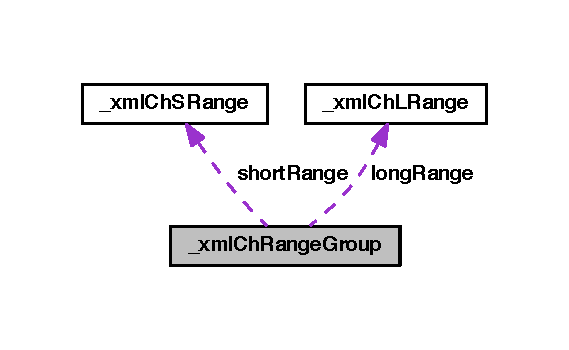
\includegraphics[width=273pt]{struct__xml_ch_range_group__coll__graph}
\end{center}
\end{figure}
\subsection*{Public Attributes}
\begin{DoxyCompactItemize}
\item 
\hypertarget{struct__xml_ch_range_group_a586ec6ff0df5781a799120268c917581}{int {\bfseries nb\-Short\-Range}}\label{struct__xml_ch_range_group_a586ec6ff0df5781a799120268c917581}

\item 
\hypertarget{struct__xml_ch_range_group_a8c00ae5937f0d5489444fd8c264f7640}{int {\bfseries nb\-Long\-Range}}\label{struct__xml_ch_range_group_a8c00ae5937f0d5489444fd8c264f7640}

\item 
\hypertarget{struct__xml_ch_range_group_ab437c33acae9b5d5d2bc8ef547baf6fe}{const \hyperlink{struct__xml_ch_s_range}{xml\-Ch\-S\-Range} $\ast$ {\bfseries short\-Range}}\label{struct__xml_ch_range_group_ab437c33acae9b5d5d2bc8ef547baf6fe}

\item 
\hypertarget{struct__xml_ch_range_group_a16b89c83778fd557add093f4235cb976}{const \hyperlink{struct__xml_ch_l_range}{xml\-Ch\-L\-Range} $\ast$ {\bfseries long\-Range}}\label{struct__xml_ch_range_group_a16b89c83778fd557add093f4235cb976}

\end{DoxyCompactItemize}


\subsection{Detailed Description}


Definition at line 44 of file chvalid.\-h.



The documentation for this struct was generated from the following files\-:\begin{DoxyCompactItemize}
\item 
Legiscode.\-applescript/build/\-Debug/\-Legiscode.\-applescript.\-app/\-Contents/\-Frameworks/libxml.\-framework/\-Versions/2.\-6.\-30/\-Headers/chvalid.\-h\item 
Legiscode.\-applescript/libxml.\-framework/\-Versions/2.\-6.\-30/\-Headers/chvalid.\-h\end{DoxyCompactItemize}

\hypertarget{struct__xml_ch_s_range}{\section{\-\_\-xml\-Ch\-S\-Range Struct Reference}
\label{struct__xml_ch_s_range}\index{\-\_\-xml\-Ch\-S\-Range@{\-\_\-xml\-Ch\-S\-Range}}
}
\subsection*{Public Attributes}
\begin{DoxyCompactItemize}
\item 
\hypertarget{struct__xml_ch_s_range_ae6678d601f260427bcad0fd8474df97d}{unsigned short {\bfseries low}}\label{struct__xml_ch_s_range_ae6678d601f260427bcad0fd8474df97d}

\item 
\hypertarget{struct__xml_ch_s_range_a050bc6f71d4bfcf455db4789ec725f1d}{unsigned short {\bfseries high}}\label{struct__xml_ch_s_range_a050bc6f71d4bfcf455db4789ec725f1d}

\end{DoxyCompactItemize}


\subsection{Detailed Description}


Definition at line 30 of file chvalid.\-h.



The documentation for this struct was generated from the following files\-:\begin{DoxyCompactItemize}
\item 
Legiscode.\-applescript/build/\-Debug/\-Legiscode.\-applescript.\-app/\-Contents/\-Frameworks/libxml.\-framework/\-Versions/2.\-6.\-30/\-Headers/chvalid.\-h\item 
Legiscode.\-applescript/libxml.\-framework/\-Versions/2.\-6.\-30/\-Headers/chvalid.\-h\end{DoxyCompactItemize}

\hypertarget{struct__xml_doc}{\section{\-\_\-xml\-Doc Struct Reference}
\label{struct__xml_doc}\index{\-\_\-xml\-Doc@{\-\_\-xml\-Doc}}
}


Collaboration diagram for \-\_\-xml\-Doc\-:
\nopagebreak
\begin{figure}[H]
\begin{center}
\leavevmode
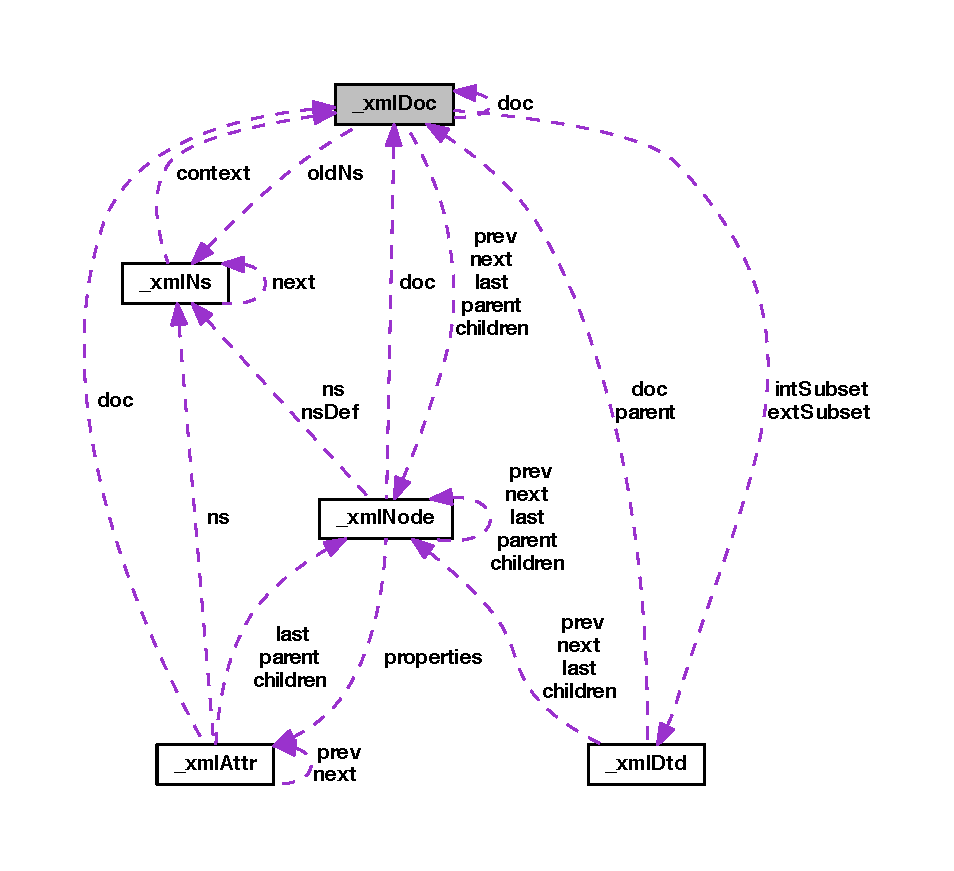
\includegraphics[width=350pt]{struct__xml_doc__coll__graph}
\end{center}
\end{figure}
\subsection*{Public Attributes}
\begin{DoxyCompactItemize}
\item 
\hypertarget{struct__xml_doc_a52b733091e8e308932f9c2c538d7a951}{void $\ast$ {\bfseries \-\_\-private}}\label{struct__xml_doc_a52b733091e8e308932f9c2c538d7a951}

\item 
\hypertarget{struct__xml_doc_aef9fa638a443a4fba932853a17948709}{xml\-Element\-Type {\bfseries type}}\label{struct__xml_doc_aef9fa638a443a4fba932853a17948709}

\item 
\hypertarget{struct__xml_doc_afdba17bb9c35668a280d1b7049ea5163}{char $\ast$ {\bfseries name}}\label{struct__xml_doc_afdba17bb9c35668a280d1b7049ea5163}

\item 
\hypertarget{struct__xml_doc_a9fac3da6377d60207a3754cd15a17082}{struct \hyperlink{struct__xml_node}{\-\_\-xml\-Node} $\ast$ {\bfseries children}}\label{struct__xml_doc_a9fac3da6377d60207a3754cd15a17082}

\item 
\hypertarget{struct__xml_doc_a4160d4424ddaae8623ed9de9bba70ed0}{struct \hyperlink{struct__xml_node}{\-\_\-xml\-Node} $\ast$ {\bfseries last}}\label{struct__xml_doc_a4160d4424ddaae8623ed9de9bba70ed0}

\item 
\hypertarget{struct__xml_doc_a5e6f10bc98067cfdb78647cc235bce92}{struct \hyperlink{struct__xml_node}{\-\_\-xml\-Node} $\ast$ {\bfseries parent}}\label{struct__xml_doc_a5e6f10bc98067cfdb78647cc235bce92}

\item 
\hypertarget{struct__xml_doc_a52143114b661e234c8b9bc3eecdb5922}{struct \hyperlink{struct__xml_node}{\-\_\-xml\-Node} $\ast$ {\bfseries next}}\label{struct__xml_doc_a52143114b661e234c8b9bc3eecdb5922}

\item 
\hypertarget{struct__xml_doc_a80c57ad5f2398896032e7349d163d529}{struct \hyperlink{struct__xml_node}{\-\_\-xml\-Node} $\ast$ {\bfseries prev}}\label{struct__xml_doc_a80c57ad5f2398896032e7349d163d529}

\item 
\hypertarget{struct__xml_doc_a56626249e933a92b9f3dc9f529a0c4ad}{struct \hyperlink{struct__xml_doc}{\-\_\-xml\-Doc} $\ast$ {\bfseries doc}}\label{struct__xml_doc_a56626249e933a92b9f3dc9f529a0c4ad}

\item 
\hypertarget{struct__xml_doc_ad4d34773df893b9823a78b011a3dbb3c}{int {\bfseries compression}}\label{struct__xml_doc_ad4d34773df893b9823a78b011a3dbb3c}

\item 
\hypertarget{struct__xml_doc_aae15c09e02b6374b357a588002515de8}{int {\bfseries standalone}}\label{struct__xml_doc_aae15c09e02b6374b357a588002515de8}

\item 
\hypertarget{struct__xml_doc_a8c7be011f3f0bcac274c6cb45115845b}{struct \hyperlink{struct__xml_dtd}{\-\_\-xml\-Dtd} $\ast$ {\bfseries int\-Subset}}\label{struct__xml_doc_a8c7be011f3f0bcac274c6cb45115845b}

\item 
\hypertarget{struct__xml_doc_a0c6c065dc87076d767a856d96013c4d4}{struct \hyperlink{struct__xml_dtd}{\-\_\-xml\-Dtd} $\ast$ {\bfseries ext\-Subset}}\label{struct__xml_doc_a0c6c065dc87076d767a856d96013c4d4}

\item 
\hypertarget{struct__xml_doc_afd462ad6f609721625a077cfd93eb059}{struct \hyperlink{struct__xml_ns}{\-\_\-xml\-Ns} $\ast$ {\bfseries old\-Ns}}\label{struct__xml_doc_afd462ad6f609721625a077cfd93eb059}

\item 
\hypertarget{struct__xml_doc_aaed3f54fe0653b95b5762c853f181201}{const xml\-Char $\ast$ {\bfseries version}}\label{struct__xml_doc_aaed3f54fe0653b95b5762c853f181201}

\item 
\hypertarget{struct__xml_doc_a466de69daa68efaa4873a2c9c5734693}{const xml\-Char $\ast$ {\bfseries encoding}}\label{struct__xml_doc_a466de69daa68efaa4873a2c9c5734693}

\item 
\hypertarget{struct__xml_doc_a7c2a0afd6fa64ed2d0171232c1a89a44}{void $\ast$ {\bfseries ids}}\label{struct__xml_doc_a7c2a0afd6fa64ed2d0171232c1a89a44}

\item 
\hypertarget{struct__xml_doc_adef74db15b1e37214cc1601f44585602}{void $\ast$ {\bfseries refs}}\label{struct__xml_doc_adef74db15b1e37214cc1601f44585602}

\item 
\hypertarget{struct__xml_doc_a87a881cb3bcc77cf04d31c12b7a47eda}{const xml\-Char $\ast$ {\bfseries U\-R\-L}}\label{struct__xml_doc_a87a881cb3bcc77cf04d31c12b7a47eda}

\item 
\hypertarget{struct__xml_doc_a32382a4784bbd3d6c928d8cd7349305b}{int {\bfseries charset}}\label{struct__xml_doc_a32382a4784bbd3d6c928d8cd7349305b}

\item 
\hypertarget{struct__xml_doc_a6aeb8db4204b026b2b6e3f929c93cce3}{struct \-\_\-xml\-Dict $\ast$ {\bfseries dict}}\label{struct__xml_doc_a6aeb8db4204b026b2b6e3f929c93cce3}

\item 
\hypertarget{struct__xml_doc_ab2ccdd867c2228625f8a008c1b912002}{void $\ast$ {\bfseries psvi}}\label{struct__xml_doc_ab2ccdd867c2228625f8a008c1b912002}

\end{DoxyCompactItemize}


\subsection{Detailed Description}


Definition at line 493 of file tree.\-h.



The documentation for this struct was generated from the following files\-:\begin{DoxyCompactItemize}
\item 
Legiscode.\-applescript/build/\-Debug/\-Legiscode.\-applescript.\-app/\-Contents/\-Frameworks/libxml.\-framework/\-Versions/2.\-6.\-30/\-Headers/tree.\-h\item 
Legiscode.\-applescript/libxml.\-framework/\-Versions/2.\-6.\-30/\-Headers/tree.\-h\end{DoxyCompactItemize}

\hypertarget{struct__xml_d_o_m_wrap_ctxt}{\section{\-\_\-xml\-D\-O\-M\-Wrap\-Ctxt Struct Reference}
\label{struct__xml_d_o_m_wrap_ctxt}\index{\-\_\-xml\-D\-O\-M\-Wrap\-Ctxt@{\-\_\-xml\-D\-O\-M\-Wrap\-Ctxt}}
}


{\ttfamily \#include $<$tree.\-h$>$}



Collaboration diagram for \-\_\-xml\-D\-O\-M\-Wrap\-Ctxt\-:
\nopagebreak
\begin{figure}[H]
\begin{center}
\leavevmode
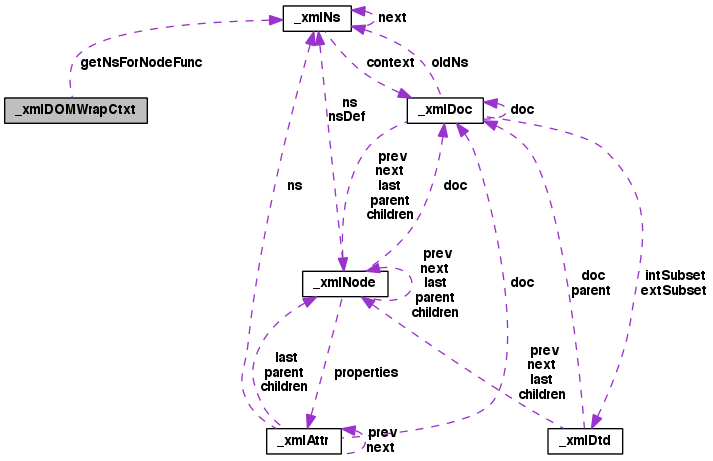
\includegraphics[width=350pt]{struct__xml_d_o_m_wrap_ctxt__coll__graph}
\end{center}
\end{figure}
\subsection*{Public Attributes}
\begin{DoxyCompactItemize}
\item 
\hypertarget{struct__xml_d_o_m_wrap_ctxt_a6edb4ec2526ffa6b6fb8953f07631b92}{void $\ast$ {\bfseries \-\_\-private}}\label{struct__xml_d_o_m_wrap_ctxt_a6edb4ec2526ffa6b6fb8953f07631b92}

\item 
\hypertarget{struct__xml_d_o_m_wrap_ctxt_a1d84b623242d09de1c0ea065e5411fbc}{int {\bfseries type}}\label{struct__xml_d_o_m_wrap_ctxt_a1d84b623242d09de1c0ea065e5411fbc}

\item 
\hypertarget{struct__xml_d_o_m_wrap_ctxt_a02a32279ef2bf5905a81dde8ec72b469}{void $\ast$ {\bfseries namespace\-Map}}\label{struct__xml_d_o_m_wrap_ctxt_a02a32279ef2bf5905a81dde8ec72b469}

\item 
\hypertarget{struct__xml_d_o_m_wrap_ctxt_a2fc065d32c83c5d1cdbd49f8162c7340}{xml\-D\-O\-M\-Wrap\-Acquire\-Ns\-Function {\bfseries get\-Ns\-For\-Node\-Func}}\label{struct__xml_d_o_m_wrap_ctxt_a2fc065d32c83c5d1cdbd49f8162c7340}

\end{DoxyCompactItemize}


\subsection{Detailed Description}
xml\-D\-O\-M\-Wrap\-Ctxt\-:

Context for D\-O\-M wrapper-\/operations. 

Definition at line 551 of file tree.\-h.



The documentation for this struct was generated from the following files\-:\begin{DoxyCompactItemize}
\item 
Legiscode.\-applescript/build/\-Debug/\-Legiscode.\-applescript.\-app/\-Contents/\-Frameworks/libxml.\-framework/\-Versions/2.\-6.\-30/\-Headers/tree.\-h\item 
Legiscode.\-applescript/libxml.\-framework/\-Versions/2.\-6.\-30/\-Headers/tree.\-h\end{DoxyCompactItemize}

\hypertarget{struct__xml_dtd}{\section{\-\_\-xml\-Dtd Struct Reference}
\label{struct__xml_dtd}\index{\-\_\-xml\-Dtd@{\-\_\-xml\-Dtd}}
}


Collaboration diagram for \-\_\-xml\-Dtd\-:
\nopagebreak
\begin{figure}[H]
\begin{center}
\leavevmode
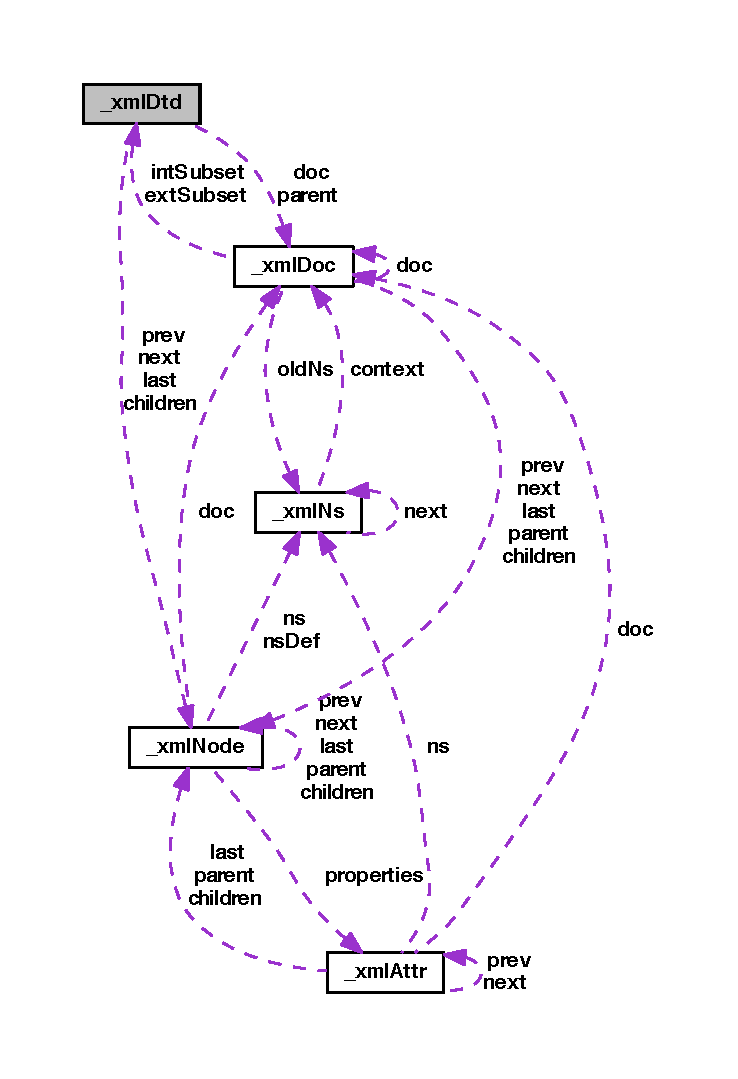
\includegraphics[width=350pt]{struct__xml_dtd__coll__graph}
\end{center}
\end{figure}
\subsection*{Public Attributes}
\begin{DoxyCompactItemize}
\item 
\hypertarget{struct__xml_dtd_abe6b7a89defa90b267043730846278df}{void $\ast$ {\bfseries \-\_\-private}}\label{struct__xml_dtd_abe6b7a89defa90b267043730846278df}

\item 
\hypertarget{struct__xml_dtd_a823418c1633bafc9bb653ddb4228bb1b}{xml\-Element\-Type {\bfseries type}}\label{struct__xml_dtd_a823418c1633bafc9bb653ddb4228bb1b}

\item 
\hypertarget{struct__xml_dtd_a78c918dca4f0ebd8ba2112953311a4ab}{const xml\-Char $\ast$ {\bfseries name}}\label{struct__xml_dtd_a78c918dca4f0ebd8ba2112953311a4ab}

\item 
\hypertarget{struct__xml_dtd_a5a0f2fee625df3f7e2d6a58c0d653a43}{struct \hyperlink{struct__xml_node}{\-\_\-xml\-Node} $\ast$ {\bfseries children}}\label{struct__xml_dtd_a5a0f2fee625df3f7e2d6a58c0d653a43}

\item 
\hypertarget{struct__xml_dtd_ade96b5fa894f9cf4ece24d987bc63811}{struct \hyperlink{struct__xml_node}{\-\_\-xml\-Node} $\ast$ {\bfseries last}}\label{struct__xml_dtd_ade96b5fa894f9cf4ece24d987bc63811}

\item 
\hypertarget{struct__xml_dtd_a3e6cbbb1a1ecde9f4b5b7835b67ea033}{struct \hyperlink{struct__xml_doc}{\-\_\-xml\-Doc} $\ast$ {\bfseries parent}}\label{struct__xml_dtd_a3e6cbbb1a1ecde9f4b5b7835b67ea033}

\item 
\hypertarget{struct__xml_dtd_a81a8e0908258bbcd1eaaf9f70541edb7}{struct \hyperlink{struct__xml_node}{\-\_\-xml\-Node} $\ast$ {\bfseries next}}\label{struct__xml_dtd_a81a8e0908258bbcd1eaaf9f70541edb7}

\item 
\hypertarget{struct__xml_dtd_af3f30e7f3d1028c9f258ac86c31578cb}{struct \hyperlink{struct__xml_node}{\-\_\-xml\-Node} $\ast$ {\bfseries prev}}\label{struct__xml_dtd_af3f30e7f3d1028c9f258ac86c31578cb}

\item 
\hypertarget{struct__xml_dtd_a5d81bc0f4970f85b316bfb0f42583486}{struct \hyperlink{struct__xml_doc}{\-\_\-xml\-Doc} $\ast$ {\bfseries doc}}\label{struct__xml_dtd_a5d81bc0f4970f85b316bfb0f42583486}

\item 
\hypertarget{struct__xml_dtd_a7b1a5c67208686bae414032e606597a2}{void $\ast$ {\bfseries notations}}\label{struct__xml_dtd_a7b1a5c67208686bae414032e606597a2}

\item 
\hypertarget{struct__xml_dtd_a27aaaa27624c73794e0dc19793929727}{void $\ast$ {\bfseries elements}}\label{struct__xml_dtd_a27aaaa27624c73794e0dc19793929727}

\item 
\hypertarget{struct__xml_dtd_acb03ef64b13d10880740d9281489c476}{void $\ast$ {\bfseries attributes}}\label{struct__xml_dtd_acb03ef64b13d10880740d9281489c476}

\item 
\hypertarget{struct__xml_dtd_a614c518b89ce0bed5677cb29ae6e6db6}{void $\ast$ {\bfseries entities}}\label{struct__xml_dtd_a614c518b89ce0bed5677cb29ae6e6db6}

\item 
\hypertarget{struct__xml_dtd_aea5fe5f6bcb04bd134c673b07b5d749e}{const xml\-Char $\ast$ {\bfseries External\-I\-D}}\label{struct__xml_dtd_aea5fe5f6bcb04bd134c673b07b5d749e}

\item 
\hypertarget{struct__xml_dtd_a929625de7d3ef6c92ec6380dbf90f0e0}{const xml\-Char $\ast$ {\bfseries System\-I\-D}}\label{struct__xml_dtd_a929625de7d3ef6c92ec6380dbf90f0e0}

\item 
\hypertarget{struct__xml_dtd_a772702228419a2a6b51a1393f2f0f010}{void $\ast$ {\bfseries pentities}}\label{struct__xml_dtd_a772702228419a2a6b51a1393f2f0f010}

\end{DoxyCompactItemize}


\subsection{Detailed Description}


Definition at line 365 of file tree.\-h.



The documentation for this struct was generated from the following files\-:\begin{DoxyCompactItemize}
\item 
Legiscode.\-applescript/build/\-Debug/\-Legiscode.\-applescript.\-app/\-Contents/\-Frameworks/libxml.\-framework/\-Versions/2.\-6.\-30/\-Headers/tree.\-h\item 
Legiscode.\-applescript/libxml.\-framework/\-Versions/2.\-6.\-30/\-Headers/tree.\-h\end{DoxyCompactItemize}

\hypertarget{struct__xml_element}{\section{\-\_\-xml\-Element Struct Reference}
\label{struct__xml_element}\index{\-\_\-xml\-Element@{\-\_\-xml\-Element}}
}


Collaboration diagram for \-\_\-xml\-Element\-:
\nopagebreak
\begin{figure}[H]
\begin{center}
\leavevmode
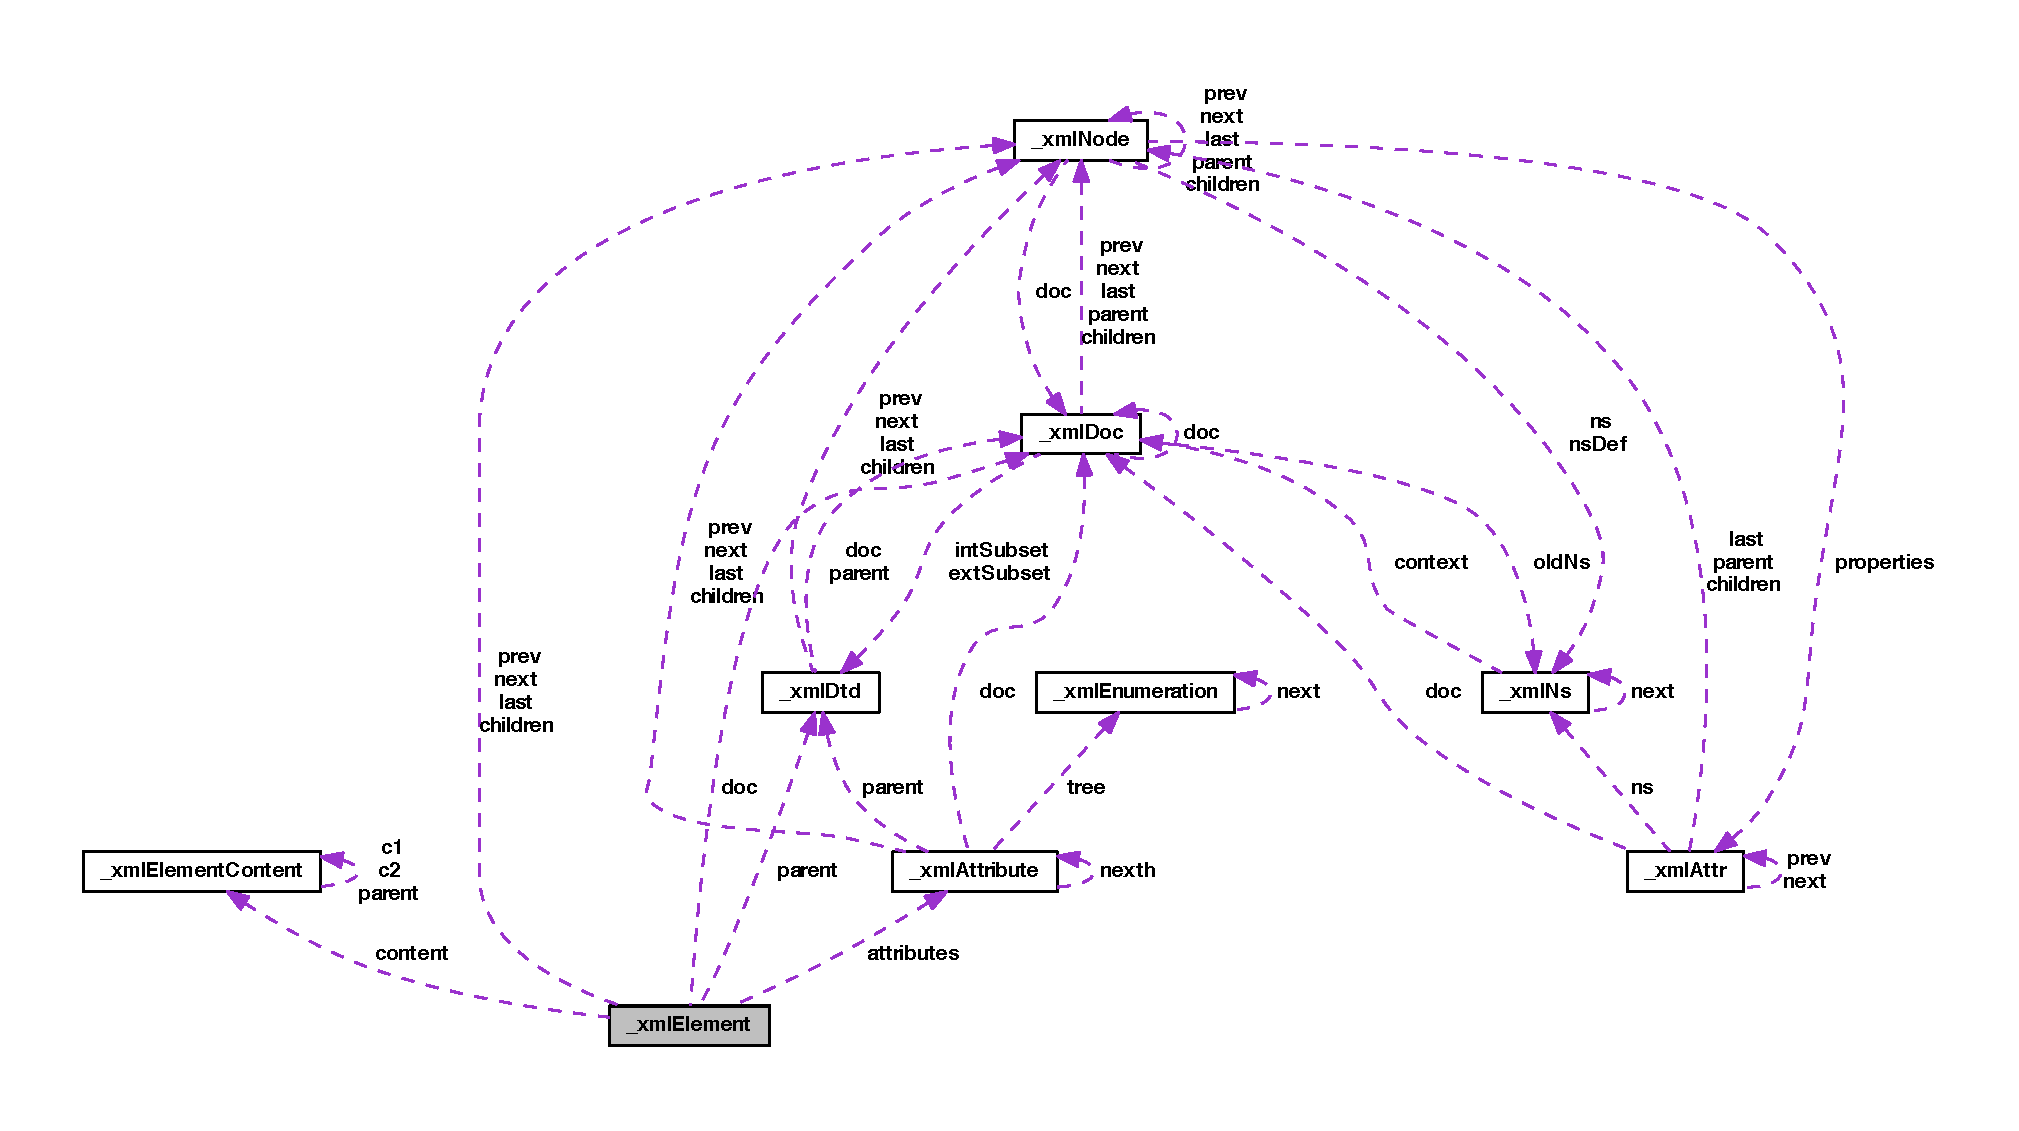
\includegraphics[width=350pt]{struct__xml_element__coll__graph}
\end{center}
\end{figure}
\subsection*{Public Attributes}
\begin{DoxyCompactItemize}
\item 
\hypertarget{struct__xml_element_acec57fd86a5831ad37b81fb56c1cc19c}{void $\ast$ {\bfseries \-\_\-private}}\label{struct__xml_element_acec57fd86a5831ad37b81fb56c1cc19c}

\item 
\hypertarget{struct__xml_element_ac73d23a5babfe6a4c48154cece65cecb}{xml\-Element\-Type {\bfseries type}}\label{struct__xml_element_ac73d23a5babfe6a4c48154cece65cecb}

\item 
\hypertarget{struct__xml_element_a5776b520d9876097d6addc1fae38ec59}{const xml\-Char $\ast$ {\bfseries name}}\label{struct__xml_element_a5776b520d9876097d6addc1fae38ec59}

\item 
\hypertarget{struct__xml_element_aac984b329d3074cf2c85579df1e1fc99}{struct \hyperlink{struct__xml_node}{\-\_\-xml\-Node} $\ast$ {\bfseries children}}\label{struct__xml_element_aac984b329d3074cf2c85579df1e1fc99}

\item 
\hypertarget{struct__xml_element_a31176322d90f7dac3ea452f03a1d6306}{struct \hyperlink{struct__xml_node}{\-\_\-xml\-Node} $\ast$ {\bfseries last}}\label{struct__xml_element_a31176322d90f7dac3ea452f03a1d6306}

\item 
\hypertarget{struct__xml_element_a470004544b490a26ae3f1e6aa6565d60}{struct \hyperlink{struct__xml_dtd}{\-\_\-xml\-Dtd} $\ast$ {\bfseries parent}}\label{struct__xml_element_a470004544b490a26ae3f1e6aa6565d60}

\item 
\hypertarget{struct__xml_element_a1a7b08d70dee7a7a7a7db63e37b27ff2}{struct \hyperlink{struct__xml_node}{\-\_\-xml\-Node} $\ast$ {\bfseries next}}\label{struct__xml_element_a1a7b08d70dee7a7a7a7db63e37b27ff2}

\item 
\hypertarget{struct__xml_element_aad487041ea7ba58be5c94f5cf8d7a8da}{struct \hyperlink{struct__xml_node}{\-\_\-xml\-Node} $\ast$ {\bfseries prev}}\label{struct__xml_element_aad487041ea7ba58be5c94f5cf8d7a8da}

\item 
\hypertarget{struct__xml_element_a23189b9512840d24e6e67cc73602aa48}{struct \hyperlink{struct__xml_doc}{\-\_\-xml\-Doc} $\ast$ {\bfseries doc}}\label{struct__xml_element_a23189b9512840d24e6e67cc73602aa48}

\item 
\hypertarget{struct__xml_element_a3f7566085877a63b728c8596438a9540}{xml\-Element\-Type\-Val {\bfseries etype}}\label{struct__xml_element_a3f7566085877a63b728c8596438a9540}

\item 
\hypertarget{struct__xml_element_ac934ce51a0a220c511c1700c3694e0e7}{\hyperlink{struct__xml_element_content}{xml\-Element\-Content\-Ptr} {\bfseries content}}\label{struct__xml_element_ac934ce51a0a220c511c1700c3694e0e7}

\item 
\hypertarget{struct__xml_element_a45468a87059e899da068a6cc04e6a943}{\hyperlink{struct__xml_attribute}{xml\-Attribute\-Ptr} {\bfseries attributes}}\label{struct__xml_element_a45468a87059e899da068a6cc04e6a943}

\item 
\hypertarget{struct__xml_element_a41bb035111f2b0b09a5833e3f63b4bfb}{const xml\-Char $\ast$ {\bfseries prefix}}\label{struct__xml_element_a41bb035111f2b0b09a5833e3f63b4bfb}

\item 
\hypertarget{struct__xml_element_a7a118861be0a195be08732cc67fd7037}{void $\ast$ {\bfseries cont\-Model}}\label{struct__xml_element_a7a118861be0a195be08732cc67fd7037}

\end{DoxyCompactItemize}


\subsection{Detailed Description}


Definition at line 305 of file tree.\-h.



The documentation for this struct was generated from the following files\-:\begin{DoxyCompactItemize}
\item 
Legiscode.\-applescript/build/\-Debug/\-Legiscode.\-applescript.\-app/\-Contents/\-Frameworks/libxml.\-framework/\-Versions/2.\-6.\-30/\-Headers/tree.\-h\item 
Legiscode.\-applescript/libxml.\-framework/\-Versions/2.\-6.\-30/\-Headers/tree.\-h\end{DoxyCompactItemize}

\hypertarget{struct__xml_element_content}{\section{\-\_\-xml\-Element\-Content Struct Reference}
\label{struct__xml_element_content}\index{\-\_\-xml\-Element\-Content@{\-\_\-xml\-Element\-Content}}
}


Collaboration diagram for \-\_\-xml\-Element\-Content\-:
\nopagebreak
\begin{figure}[H]
\begin{center}
\leavevmode
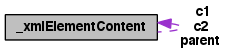
\includegraphics[width=242pt]{struct__xml_element_content__coll__graph}
\end{center}
\end{figure}
\subsection*{Public Attributes}
\begin{DoxyCompactItemize}
\item 
\hypertarget{struct__xml_element_content_a9ec31227deddf6cb534eaba958cc8a2a}{xml\-Element\-Content\-Type {\bfseries type}}\label{struct__xml_element_content_a9ec31227deddf6cb534eaba958cc8a2a}

\item 
\hypertarget{struct__xml_element_content_a45c3092e58963270a4c9640016b61ce3}{xml\-Element\-Content\-Occur {\bfseries ocur}}\label{struct__xml_element_content_a45c3092e58963270a4c9640016b61ce3}

\item 
\hypertarget{struct__xml_element_content_a3c814e1fcce494db3382965fee367342}{const xml\-Char $\ast$ {\bfseries name}}\label{struct__xml_element_content_a3c814e1fcce494db3382965fee367342}

\item 
\hypertarget{struct__xml_element_content_a79213e3823ffdba5e810539cecc0ba7b}{struct \hyperlink{struct__xml_element_content}{\-\_\-xml\-Element\-Content} $\ast$ {\bfseries c1}}\label{struct__xml_element_content_a79213e3823ffdba5e810539cecc0ba7b}

\item 
\hypertarget{struct__xml_element_content_a0e3adfa5e9910fa37bc302d66b254600}{struct \hyperlink{struct__xml_element_content}{\-\_\-xml\-Element\-Content} $\ast$ {\bfseries c2}}\label{struct__xml_element_content_a0e3adfa5e9910fa37bc302d66b254600}

\item 
\hypertarget{struct__xml_element_content_afc9791f9c8604d8232b98cccc1fa19cd}{struct \hyperlink{struct__xml_element_content}{\-\_\-xml\-Element\-Content} $\ast$ {\bfseries parent}}\label{struct__xml_element_content_afc9791f9c8604d8232b98cccc1fa19cd}

\item 
\hypertarget{struct__xml_element_content_a53d312c5dd947160bcbf5da8c6a2f4da}{const xml\-Char $\ast$ {\bfseries prefix}}\label{struct__xml_element_content_a53d312c5dd947160bcbf5da8c6a2f4da}

\end{DoxyCompactItemize}


\subsection{Detailed Description}


Definition at line 265 of file tree.\-h.



The documentation for this struct was generated from the following files\-:\begin{DoxyCompactItemize}
\item 
Legiscode.\-applescript/build/\-Debug/\-Legiscode.\-applescript.\-app/\-Contents/\-Frameworks/libxml.\-framework/\-Versions/2.\-6.\-30/\-Headers/tree.\-h\item 
Legiscode.\-applescript/libxml.\-framework/\-Versions/2.\-6.\-30/\-Headers/tree.\-h\end{DoxyCompactItemize}

\hypertarget{struct__xml_entity}{\section{\-\_\-xml\-Entity Struct Reference}
\label{struct__xml_entity}\index{\-\_\-xml\-Entity@{\-\_\-xml\-Entity}}
}


Collaboration diagram for \-\_\-xml\-Entity\-:
\nopagebreak
\begin{figure}[H]
\begin{center}
\leavevmode
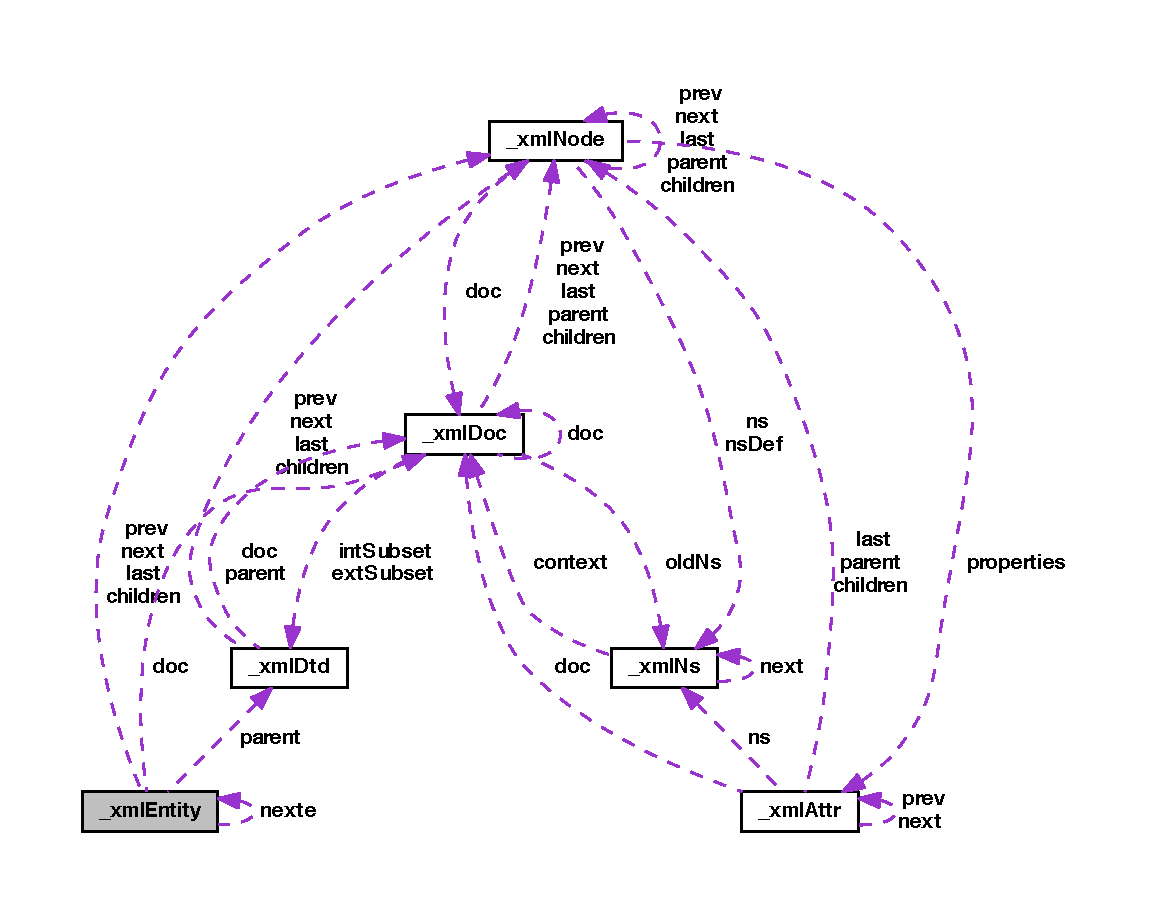
\includegraphics[width=350pt]{struct__xml_entity__coll__graph}
\end{center}
\end{figure}
\subsection*{Public Attributes}
\begin{DoxyCompactItemize}
\item 
\hypertarget{struct__xml_entity_a7e6b204a86c61fed2487a4a5fa812023}{void $\ast$ {\bfseries \-\_\-private}}\label{struct__xml_entity_a7e6b204a86c61fed2487a4a5fa812023}

\item 
\hypertarget{struct__xml_entity_ac3b4e1ec2a9713ed75c05395c925f994}{xml\-Element\-Type {\bfseries type}}\label{struct__xml_entity_ac3b4e1ec2a9713ed75c05395c925f994}

\item 
\hypertarget{struct__xml_entity_ab9efc1e9306ec1287447398af6c99a10}{const xml\-Char $\ast$ {\bfseries name}}\label{struct__xml_entity_ab9efc1e9306ec1287447398af6c99a10}

\item 
\hypertarget{struct__xml_entity_a8f9c363a4ee2977aa282302531e5e93e}{struct \hyperlink{struct__xml_node}{\-\_\-xml\-Node} $\ast$ {\bfseries children}}\label{struct__xml_entity_a8f9c363a4ee2977aa282302531e5e93e}

\item 
\hypertarget{struct__xml_entity_a34130853e77da803d3f3280f4e21ae99}{struct \hyperlink{struct__xml_node}{\-\_\-xml\-Node} $\ast$ {\bfseries last}}\label{struct__xml_entity_a34130853e77da803d3f3280f4e21ae99}

\item 
\hypertarget{struct__xml_entity_a9a01bb0bf68a58e65c75f2902bbb2938}{struct \hyperlink{struct__xml_dtd}{\-\_\-xml\-Dtd} $\ast$ {\bfseries parent}}\label{struct__xml_entity_a9a01bb0bf68a58e65c75f2902bbb2938}

\item 
\hypertarget{struct__xml_entity_af10dc2b647b69cdef189263a0d1acf9c}{struct \hyperlink{struct__xml_node}{\-\_\-xml\-Node} $\ast$ {\bfseries next}}\label{struct__xml_entity_af10dc2b647b69cdef189263a0d1acf9c}

\item 
\hypertarget{struct__xml_entity_a1be59b93b411f92997cd5e0d5000ae1f}{struct \hyperlink{struct__xml_node}{\-\_\-xml\-Node} $\ast$ {\bfseries prev}}\label{struct__xml_entity_a1be59b93b411f92997cd5e0d5000ae1f}

\item 
\hypertarget{struct__xml_entity_abc2ced859cdce7e919a704b0f5937f48}{struct \hyperlink{struct__xml_doc}{\-\_\-xml\-Doc} $\ast$ {\bfseries doc}}\label{struct__xml_entity_abc2ced859cdce7e919a704b0f5937f48}

\item 
\hypertarget{struct__xml_entity_a4fbee9532ab68f3fb934cddbd334f5f0}{xml\-Char $\ast$ {\bfseries orig}}\label{struct__xml_entity_a4fbee9532ab68f3fb934cddbd334f5f0}

\item 
\hypertarget{struct__xml_entity_a92fe8392cdd59e729fc3775c9978322e}{xml\-Char $\ast$ {\bfseries content}}\label{struct__xml_entity_a92fe8392cdd59e729fc3775c9978322e}

\item 
\hypertarget{struct__xml_entity_a2be272ed0fa826273581be4342e8c1aa}{int {\bfseries length}}\label{struct__xml_entity_a2be272ed0fa826273581be4342e8c1aa}

\item 
\hypertarget{struct__xml_entity_a7c77f01ae8584f35322960c9af2c44f1}{xml\-Entity\-Type {\bfseries etype}}\label{struct__xml_entity_a7c77f01ae8584f35322960c9af2c44f1}

\item 
\hypertarget{struct__xml_entity_a5d10c3fe8508367fed9864075a4c2706}{const xml\-Char $\ast$ {\bfseries External\-I\-D}}\label{struct__xml_entity_a5d10c3fe8508367fed9864075a4c2706}

\item 
\hypertarget{struct__xml_entity_a12a730dae9c09b0af92ed9b608f0c1de}{const xml\-Char $\ast$ {\bfseries System\-I\-D}}\label{struct__xml_entity_a12a730dae9c09b0af92ed9b608f0c1de}

\item 
\hypertarget{struct__xml_entity_a452b59087e9ef4bf52d4d068bb7caece}{struct \hyperlink{struct__xml_entity}{\-\_\-xml\-Entity} $\ast$ {\bfseries nexte}}\label{struct__xml_entity_a452b59087e9ef4bf52d4d068bb7caece}

\item 
\hypertarget{struct__xml_entity_a7f1e9e34a5d9a8d0c1e741625cd68a76}{const xml\-Char $\ast$ {\bfseries U\-R\-I}}\label{struct__xml_entity_a7f1e9e34a5d9a8d0c1e741625cd68a76}

\item 
\hypertarget{struct__xml_entity_ae649c00dd7685e9ec5cdc8e907fb62e7}{int {\bfseries owner}}\label{struct__xml_entity_ae649c00dd7685e9ec5cdc8e907fb62e7}

\item 
\hypertarget{struct__xml_entity_a8d02912e453726ef10dce4e48dd7ba78}{int {\bfseries checked}}\label{struct__xml_entity_a8d02912e453726ef10dce4e48dd7ba78}

\end{DoxyCompactItemize}


\subsection{Detailed Description}


Definition at line 38 of file entities.\-h.



The documentation for this struct was generated from the following files\-:\begin{DoxyCompactItemize}
\item 
Legiscode.\-applescript/build/\-Debug/\-Legiscode.\-applescript.\-app/\-Contents/\-Frameworks/libxml.\-framework/\-Versions/2.\-6.\-30/\-Headers/entities.\-h\item 
Legiscode.\-applescript/libxml.\-framework/\-Versions/2.\-6.\-30/\-Headers/entities.\-h\end{DoxyCompactItemize}

\hypertarget{struct__xml_enumeration}{\section{\-\_\-xml\-Enumeration Struct Reference}
\label{struct__xml_enumeration}\index{\-\_\-xml\-Enumeration@{\-\_\-xml\-Enumeration}}
}


Collaboration diagram for \-\_\-xml\-Enumeration\-:
\nopagebreak
\begin{figure}[H]
\begin{center}
\leavevmode
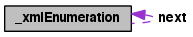
\includegraphics[width=217pt]{struct__xml_enumeration__coll__graph}
\end{center}
\end{figure}
\subsection*{Public Attributes}
\begin{DoxyCompactItemize}
\item 
\hypertarget{struct__xml_enumeration_a80fb1f362d109ee2cf01f4f6adef2b9a}{struct \hyperlink{struct__xml_enumeration}{\-\_\-xml\-Enumeration} $\ast$ {\bfseries next}}\label{struct__xml_enumeration_a80fb1f362d109ee2cf01f4f6adef2b9a}

\item 
\hypertarget{struct__xml_enumeration_a06eb8d6c0faca73ab6d7c9b0ec9a3986}{const xml\-Char $\ast$ {\bfseries name}}\label{struct__xml_enumeration_a06eb8d6c0faca73ab6d7c9b0ec9a3986}

\end{DoxyCompactItemize}


\subsection{Detailed Description}


Definition at line 199 of file tree.\-h.



The documentation for this struct was generated from the following files\-:\begin{DoxyCompactItemize}
\item 
Legiscode.\-applescript/build/\-Debug/\-Legiscode.\-applescript.\-app/\-Contents/\-Frameworks/libxml.\-framework/\-Versions/2.\-6.\-30/\-Headers/tree.\-h\item 
Legiscode.\-applescript/libxml.\-framework/\-Versions/2.\-6.\-30/\-Headers/tree.\-h\end{DoxyCompactItemize}

\input{struct__xml_error}
\hypertarget{struct__xml_global_state}{\section{\-\_\-xml\-Global\-State Struct Reference}
\label{struct__xml_global_state}\index{\-\_\-xml\-Global\-State@{\-\_\-xml\-Global\-State}}
}


Collaboration diagram for \-\_\-xml\-Global\-State\-:
\nopagebreak
\begin{figure}[H]
\begin{center}
\leavevmode
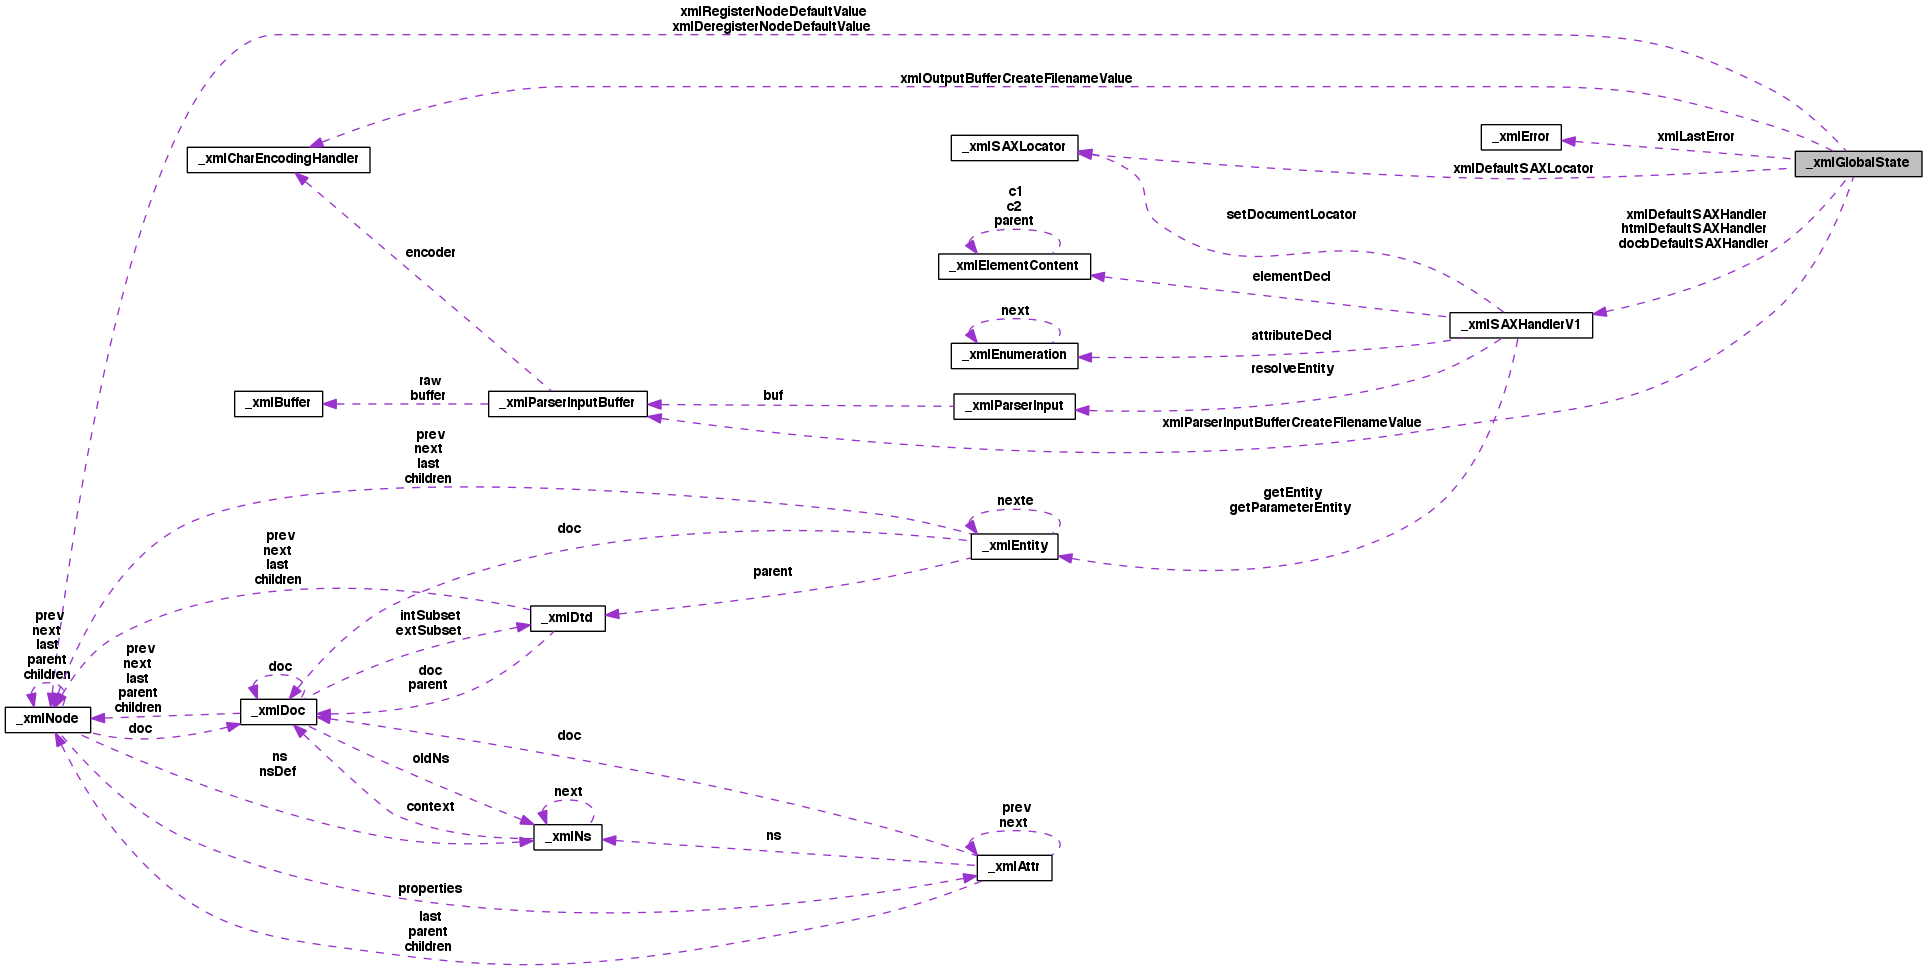
\includegraphics[width=350pt]{struct__xml_global_state__coll__graph}
\end{center}
\end{figure}
\subsection*{Public Attributes}
\begin{DoxyCompactItemize}
\item 
\hypertarget{struct__xml_global_state_a4674d4fe0ec272474d9af4918aa8e9a5}{const char $\ast$ {\bfseries xml\-Parser\-Version}}\label{struct__xml_global_state_a4674d4fe0ec272474d9af4918aa8e9a5}

\item 
\hypertarget{struct__xml_global_state_aed1adc9856d172d3de5d036f072cbb1a}{\hyperlink{struct__xml_s_a_x_locator}{xml\-S\-A\-X\-Locator} {\bfseries xml\-Default\-S\-A\-X\-Locator}}\label{struct__xml_global_state_aed1adc9856d172d3de5d036f072cbb1a}

\item 
\hypertarget{struct__xml_global_state_a256cd5324f2a89b49e0139c5c8e39ea1}{\hyperlink{struct__xml_s_a_x_handler_v1}{xml\-S\-A\-X\-Handler\-V1} {\bfseries xml\-Default\-S\-A\-X\-Handler}}\label{struct__xml_global_state_a256cd5324f2a89b49e0139c5c8e39ea1}

\item 
\hypertarget{struct__xml_global_state_a2450ebc67fb96e53f0df344907da8f48}{\hyperlink{struct__xml_s_a_x_handler_v1}{xml\-S\-A\-X\-Handler\-V1} {\bfseries docb\-Default\-S\-A\-X\-Handler}}\label{struct__xml_global_state_a2450ebc67fb96e53f0df344907da8f48}

\item 
\hypertarget{struct__xml_global_state_a07e7a66e908fa0aef7bfa9a42e1b2cb7}{\hyperlink{struct__xml_s_a_x_handler_v1}{xml\-S\-A\-X\-Handler\-V1} {\bfseries html\-Default\-S\-A\-X\-Handler}}\label{struct__xml_global_state_a07e7a66e908fa0aef7bfa9a42e1b2cb7}

\item 
\hypertarget{struct__xml_global_state_a842b3e02678910e93737a0c9c520d454}{xml\-Free\-Func {\bfseries xml\-Free}}\label{struct__xml_global_state_a842b3e02678910e93737a0c9c520d454}

\item 
\hypertarget{struct__xml_global_state_aa4f9f1f20f477d6d6b108e6ecf7c4561}{xml\-Malloc\-Func {\bfseries xml\-Malloc}}\label{struct__xml_global_state_aa4f9f1f20f477d6d6b108e6ecf7c4561}

\item 
\hypertarget{struct__xml_global_state_a480efe13ea3f6855bae2e9a9f7f3a0c2}{xml\-Strdup\-Func {\bfseries xml\-Mem\-Strdup}}\label{struct__xml_global_state_a480efe13ea3f6855bae2e9a9f7f3a0c2}

\item 
\hypertarget{struct__xml_global_state_afe3342331af0b0563377a7967ba2fa68}{xml\-Realloc\-Func {\bfseries xml\-Realloc}}\label{struct__xml_global_state_afe3342331af0b0563377a7967ba2fa68}

\item 
\hypertarget{struct__xml_global_state_a68fec3bbfc35f99f7bff04373dbf90c2}{xml\-Generic\-Error\-Func {\bfseries xml\-Generic\-Error}}\label{struct__xml_global_state_a68fec3bbfc35f99f7bff04373dbf90c2}

\item 
\hypertarget{struct__xml_global_state_aef0f8aae9672650f571ccfdb5fe893a1}{xml\-Structured\-Error\-Func {\bfseries xml\-Structured\-Error}}\label{struct__xml_global_state_aef0f8aae9672650f571ccfdb5fe893a1}

\item 
\hypertarget{struct__xml_global_state_afa3b643858b3bd1cf3c4c968501888ab}{void $\ast$ {\bfseries xml\-Generic\-Error\-Context}}\label{struct__xml_global_state_afa3b643858b3bd1cf3c4c968501888ab}

\item 
\hypertarget{struct__xml_global_state_a3a4587d5954d544f4ca2234374d3bcd9}{int {\bfseries old\-X\-M\-L\-W\-Dcompatibility}}\label{struct__xml_global_state_a3a4587d5954d544f4ca2234374d3bcd9}

\item 
\hypertarget{struct__xml_global_state_a4da43ce871efefda1a35b93cf442c553}{xml\-Buffer\-Allocation\-Scheme {\bfseries xml\-Buffer\-Alloc\-Scheme}}\label{struct__xml_global_state_a4da43ce871efefda1a35b93cf442c553}

\item 
\hypertarget{struct__xml_global_state_abb8a2b0c3484e57154ff709c7c8dc94b}{int {\bfseries xml\-Default\-Buffer\-Size}}\label{struct__xml_global_state_abb8a2b0c3484e57154ff709c7c8dc94b}

\item 
\hypertarget{struct__xml_global_state_a1a0fd78aa36e227f429299a808ea8bee}{int {\bfseries xml\-Substitute\-Entities\-Default\-Value}}\label{struct__xml_global_state_a1a0fd78aa36e227f429299a808ea8bee}

\item 
\hypertarget{struct__xml_global_state_ab94304dcd880b0c6f68634fe7fcc60ef}{int {\bfseries xml\-Do\-Validity\-Checking\-Default\-Value}}\label{struct__xml_global_state_ab94304dcd880b0c6f68634fe7fcc60ef}

\item 
\hypertarget{struct__xml_global_state_af4caac50e246cf1f1b6fc0fb9eb7ac83}{int {\bfseries xml\-Get\-Warnings\-Default\-Value}}\label{struct__xml_global_state_af4caac50e246cf1f1b6fc0fb9eb7ac83}

\item 
\hypertarget{struct__xml_global_state_aafbd2893936cc7e0b906277bf4476f26}{int {\bfseries xml\-Keep\-Blanks\-Default\-Value}}\label{struct__xml_global_state_aafbd2893936cc7e0b906277bf4476f26}

\item 
\hypertarget{struct__xml_global_state_a60edc1852ca27c7910919b2b0813f0f8}{int {\bfseries xml\-Line\-Numbers\-Default\-Value}}\label{struct__xml_global_state_a60edc1852ca27c7910919b2b0813f0f8}

\item 
\hypertarget{struct__xml_global_state_a5372304342b0799d753b848b4ff797f2}{int {\bfseries xml\-Load\-Ext\-Dtd\-Default\-Value}}\label{struct__xml_global_state_a5372304342b0799d753b848b4ff797f2}

\item 
\hypertarget{struct__xml_global_state_ab1de5b17ba7c598ab79b3f842f017c26}{int {\bfseries xml\-Parser\-Debug\-Entities}}\label{struct__xml_global_state_ab1de5b17ba7c598ab79b3f842f017c26}

\item 
\hypertarget{struct__xml_global_state_aed754d7889fb431e0d9623660db32ea3}{int {\bfseries xml\-Pedantic\-Parser\-Default\-Value}}\label{struct__xml_global_state_aed754d7889fb431e0d9623660db32ea3}

\item 
\hypertarget{struct__xml_global_state_a2e91a726bfc9552958e60c867ebb4a7b}{int {\bfseries xml\-Save\-No\-Empty\-Tags}}\label{struct__xml_global_state_a2e91a726bfc9552958e60c867ebb4a7b}

\item 
\hypertarget{struct__xml_global_state_a321904b6d88296e892ebe7120aa62ace}{int {\bfseries xml\-Indent\-Tree\-Output}}\label{struct__xml_global_state_a321904b6d88296e892ebe7120aa62ace}

\item 
\hypertarget{struct__xml_global_state_a02abcd3108a8256afc6342b364fce724}{const char $\ast$ {\bfseries xml\-Tree\-Indent\-String}}\label{struct__xml_global_state_a02abcd3108a8256afc6342b364fce724}

\item 
\hypertarget{struct__xml_global_state_a30d6034926e4292ce0feec490008c568}{xml\-Register\-Node\-Func {\bfseries xml\-Register\-Node\-Default\-Value}}\label{struct__xml_global_state_a30d6034926e4292ce0feec490008c568}

\item 
\hypertarget{struct__xml_global_state_a7dd29e256c9eeb78789c6f483bd4098b}{xml\-Deregister\-Node\-Func {\bfseries xml\-Deregister\-Node\-Default\-Value}}\label{struct__xml_global_state_a7dd29e256c9eeb78789c6f483bd4098b}

\item 
\hypertarget{struct__xml_global_state_ab2b37c13cce8ccc8a7bb0e0a47474563}{xml\-Malloc\-Func {\bfseries xml\-Malloc\-Atomic}}\label{struct__xml_global_state_ab2b37c13cce8ccc8a7bb0e0a47474563}

\item 
\hypertarget{struct__xml_global_state_afd5f9c9dc58ab8f75fb0074370e18bbb}{\hyperlink{struct__xml_error}{xml\-Error} {\bfseries xml\-Last\-Error}}\label{struct__xml_global_state_afd5f9c9dc58ab8f75fb0074370e18bbb}

\item 
\hypertarget{struct__xml_global_state_a4426a58b33b2f1db58f66c4a01d1044c}{xml\-Parser\-Input\-Buffer\-Create\-Filename\-Func {\bfseries xml\-Parser\-Input\-Buffer\-Create\-Filename\-Value}}\label{struct__xml_global_state_a4426a58b33b2f1db58f66c4a01d1044c}

\item 
\hypertarget{struct__xml_global_state_ad9c2ba58bc1b222cd1189a265a137276}{xml\-Output\-Buffer\-Create\-Filename\-Func {\bfseries xml\-Output\-Buffer\-Create\-Filename\-Value}}\label{struct__xml_global_state_ad9c2ba58bc1b222cd1189a265a137276}

\end{DoxyCompactItemize}


\subsection{Detailed Description}


Definition at line 81 of file globals.\-h.



The documentation for this struct was generated from the following files\-:\begin{DoxyCompactItemize}
\item 
Legiscode.\-applescript/build/\-Debug/\-Legiscode.\-applescript.\-app/\-Contents/\-Frameworks/libxml.\-framework/\-Versions/2.\-6.\-30/\-Headers/globals.\-h\item 
Legiscode.\-applescript/libxml.\-framework/\-Versions/2.\-6.\-30/\-Headers/globals.\-h\end{DoxyCompactItemize}

\hypertarget{struct__xml_i_d}{\section{\-\_\-xml\-I\-D Struct Reference}
\label{struct__xml_i_d}\index{\-\_\-xml\-I\-D@{\-\_\-xml\-I\-D}}
}


Collaboration diagram for \-\_\-xml\-I\-D\-:
\nopagebreak
\begin{figure}[H]
\begin{center}
\leavevmode
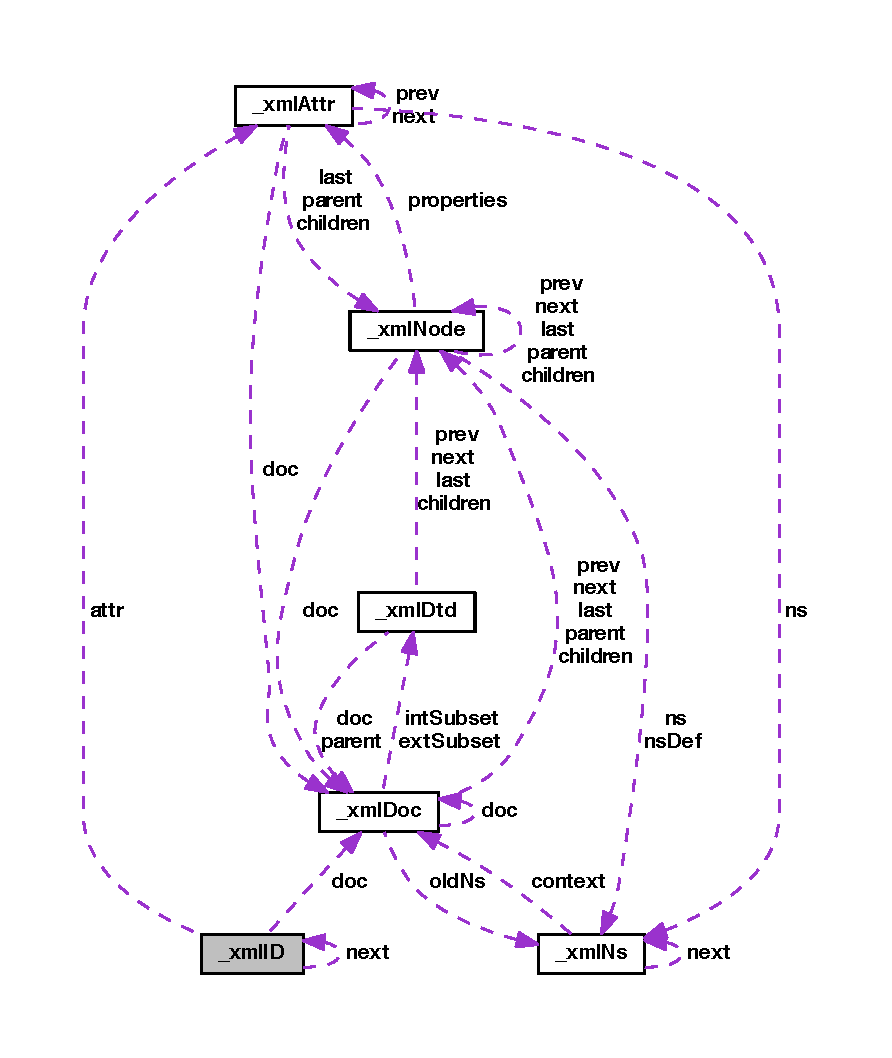
\includegraphics[width=350pt]{struct__xml_i_d__coll__graph}
\end{center}
\end{figure}
\subsection*{Public Attributes}
\begin{DoxyCompactItemize}
\item 
\hypertarget{struct__xml_i_d_a5eea0372c8976b6e6ed365818b820e26}{struct \hyperlink{struct__xml_i_d}{\-\_\-xml\-I\-D} $\ast$ {\bfseries next}}\label{struct__xml_i_d_a5eea0372c8976b6e6ed365818b820e26}

\item 
\hypertarget{struct__xml_i_d_ae0a55b852d00154a8ad1120b924160e0}{const xml\-Char $\ast$ {\bfseries value}}\label{struct__xml_i_d_ae0a55b852d00154a8ad1120b924160e0}

\item 
\hypertarget{struct__xml_i_d_a0273ce499877771549f91b374bfb6f95}{\hyperlink{struct__xml_attr}{xml\-Attr\-Ptr} {\bfseries attr}}\label{struct__xml_i_d_a0273ce499877771549f91b374bfb6f95}

\item 
\hypertarget{struct__xml_i_d_a77259e46687706750d4eee54b78f4734}{const xml\-Char $\ast$ {\bfseries name}}\label{struct__xml_i_d_a77259e46687706750d4eee54b78f4734}

\item 
\hypertarget{struct__xml_i_d_a108740dc154fd8bfedb996e6a2de419e}{int {\bfseries lineno}}\label{struct__xml_i_d_a108740dc154fd8bfedb996e6a2de419e}

\item 
\hypertarget{struct__xml_i_d_abc75a59d0b39585e97534cf2dfc4a688}{struct \hyperlink{struct__xml_doc}{\-\_\-xml\-Doc} $\ast$ {\bfseries doc}}\label{struct__xml_i_d_abc75a59d0b39585e97534cf2dfc4a688}

\end{DoxyCompactItemize}


\subsection{Detailed Description}


Definition at line 416 of file tree.\-h.



The documentation for this struct was generated from the following files\-:\begin{DoxyCompactItemize}
\item 
Legiscode.\-applescript/build/\-Debug/\-Legiscode.\-applescript.\-app/\-Contents/\-Frameworks/libxml.\-framework/\-Versions/2.\-6.\-30/\-Headers/tree.\-h\item 
Legiscode.\-applescript/libxml.\-framework/\-Versions/2.\-6.\-30/\-Headers/tree.\-h\end{DoxyCompactItemize}

\input{struct__xml_node}
\hypertarget{struct__xml_notation}{\section{\-\_\-xml\-Notation Struct Reference}
\label{struct__xml_notation}\index{\-\_\-xml\-Notation@{\-\_\-xml\-Notation}}
}
\subsection*{Public Attributes}
\begin{DoxyCompactItemize}
\item 
\hypertarget{struct__xml_notation_a696d7ee623b3fff8dbb76d397b63abf8}{const xml\-Char $\ast$ {\bfseries name}}\label{struct__xml_notation_a696d7ee623b3fff8dbb76d397b63abf8}

\item 
\hypertarget{struct__xml_notation_a37865948f9c0b13d1c2c877fce12425e}{const xml\-Char $\ast$ {\bfseries Public\-I\-D}}\label{struct__xml_notation_a37865948f9c0b13d1c2c877fce12425e}

\item 
\hypertarget{struct__xml_notation_ad9d8e72be291bd6eff7075e2a6451aac}{const xml\-Char $\ast$ {\bfseries System\-I\-D}}\label{struct__xml_notation_ad9d8e72be291bd6eff7075e2a6451aac}

\end{DoxyCompactItemize}


\subsection{Detailed Description}


Definition at line 153 of file tree.\-h.



The documentation for this struct was generated from the following files\-:\begin{DoxyCompactItemize}
\item 
Legiscode.\-applescript/build/\-Debug/\-Legiscode.\-applescript.\-app/\-Contents/\-Frameworks/libxml.\-framework/\-Versions/2.\-6.\-30/\-Headers/tree.\-h\item 
Legiscode.\-applescript/libxml.\-framework/\-Versions/2.\-6.\-30/\-Headers/tree.\-h\end{DoxyCompactItemize}

\hypertarget{struct__xml_ns}{\section{\-\_\-xml\-Ns Struct Reference}
\label{struct__xml_ns}\index{\-\_\-xml\-Ns@{\-\_\-xml\-Ns}}
}


Collaboration diagram for \-\_\-xml\-Ns\-:
\nopagebreak
\begin{figure}[H]
\begin{center}
\leavevmode
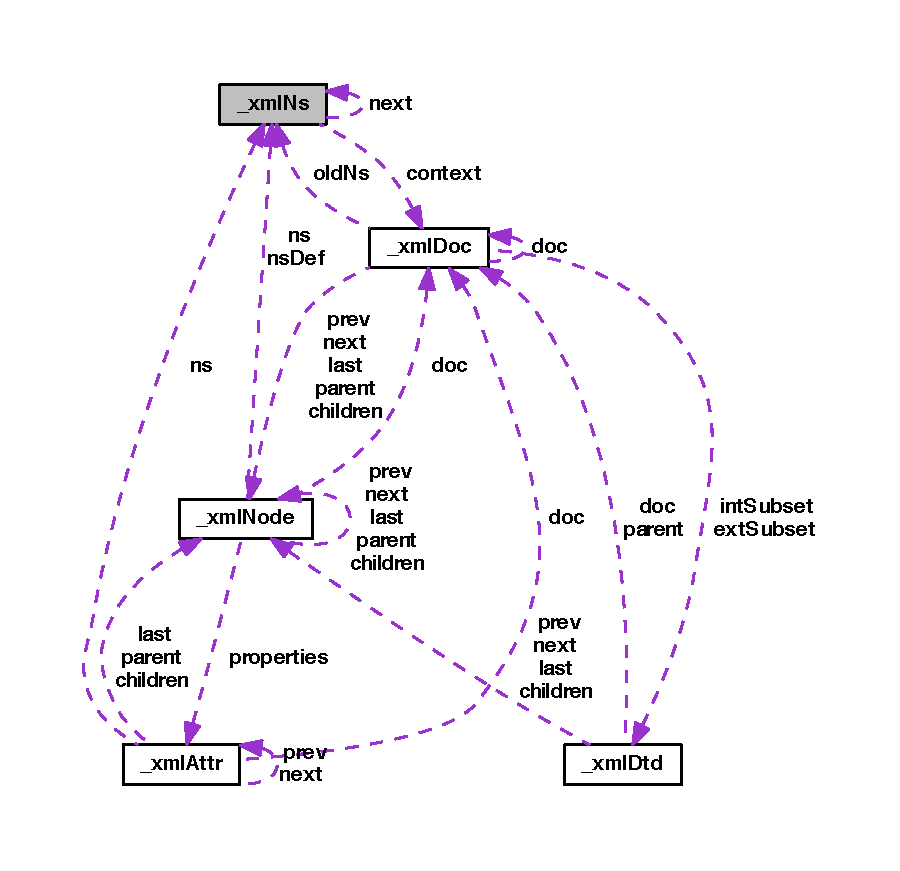
\includegraphics[width=350pt]{struct__xml_ns__coll__graph}
\end{center}
\end{figure}
\subsection*{Public Attributes}
\begin{DoxyCompactItemize}
\item 
\hypertarget{struct__xml_ns_a6f57f2718d7696076f46cec563a1f344}{struct \hyperlink{struct__xml_ns}{\-\_\-xml\-Ns} $\ast$ {\bfseries next}}\label{struct__xml_ns_a6f57f2718d7696076f46cec563a1f344}

\item 
\hypertarget{struct__xml_ns_a84c713211df0640c7cfb1e7c64149214}{xml\-Ns\-Type {\bfseries type}}\label{struct__xml_ns_a84c713211df0640c7cfb1e7c64149214}

\item 
\hypertarget{struct__xml_ns_ad9dd47dd11698ed47cc62a4c25406868}{const xml\-Char $\ast$ {\bfseries href}}\label{struct__xml_ns_ad9dd47dd11698ed47cc62a4c25406868}

\item 
\hypertarget{struct__xml_ns_a26e92982bad5ce5b1c039208bdd281d5}{const xml\-Char $\ast$ {\bfseries prefix}}\label{struct__xml_ns_a26e92982bad5ce5b1c039208bdd281d5}

\item 
\hypertarget{struct__xml_ns_ac251ddaecf66b4bc98ba61f3369e9173}{void $\ast$ {\bfseries \-\_\-private}}\label{struct__xml_ns_ac251ddaecf66b4bc98ba61f3369e9173}

\item 
\hypertarget{struct__xml_ns_ae159f51d12eef9f56610735b5b509fcc}{struct \hyperlink{struct__xml_doc}{\-\_\-xml\-Doc} $\ast$ {\bfseries context}}\label{struct__xml_ns_ae159f51d12eef9f56610735b5b509fcc}

\end{DoxyCompactItemize}


\subsection{Detailed Description}


Definition at line 348 of file tree.\-h.



The documentation for this struct was generated from the following files\-:\begin{DoxyCompactItemize}
\item 
Legiscode.\-applescript/build/\-Debug/\-Legiscode.\-applescript.\-app/\-Contents/\-Frameworks/libxml.\-framework/\-Versions/2.\-6.\-30/\-Headers/tree.\-h\item 
Legiscode.\-applescript/libxml.\-framework/\-Versions/2.\-6.\-30/\-Headers/tree.\-h\end{DoxyCompactItemize}

\hypertarget{struct__xml_parser_ctxt}{\section{\-\_\-xml\-Parser\-Ctxt Struct Reference}
\label{struct__xml_parser_ctxt}\index{\-\_\-xml\-Parser\-Ctxt@{\-\_\-xml\-Parser\-Ctxt}}
}


{\ttfamily \#include $<$parser.\-h$>$}



Collaboration diagram for \-\_\-xml\-Parser\-Ctxt\-:
\nopagebreak
\begin{figure}[H]
\begin{center}
\leavevmode
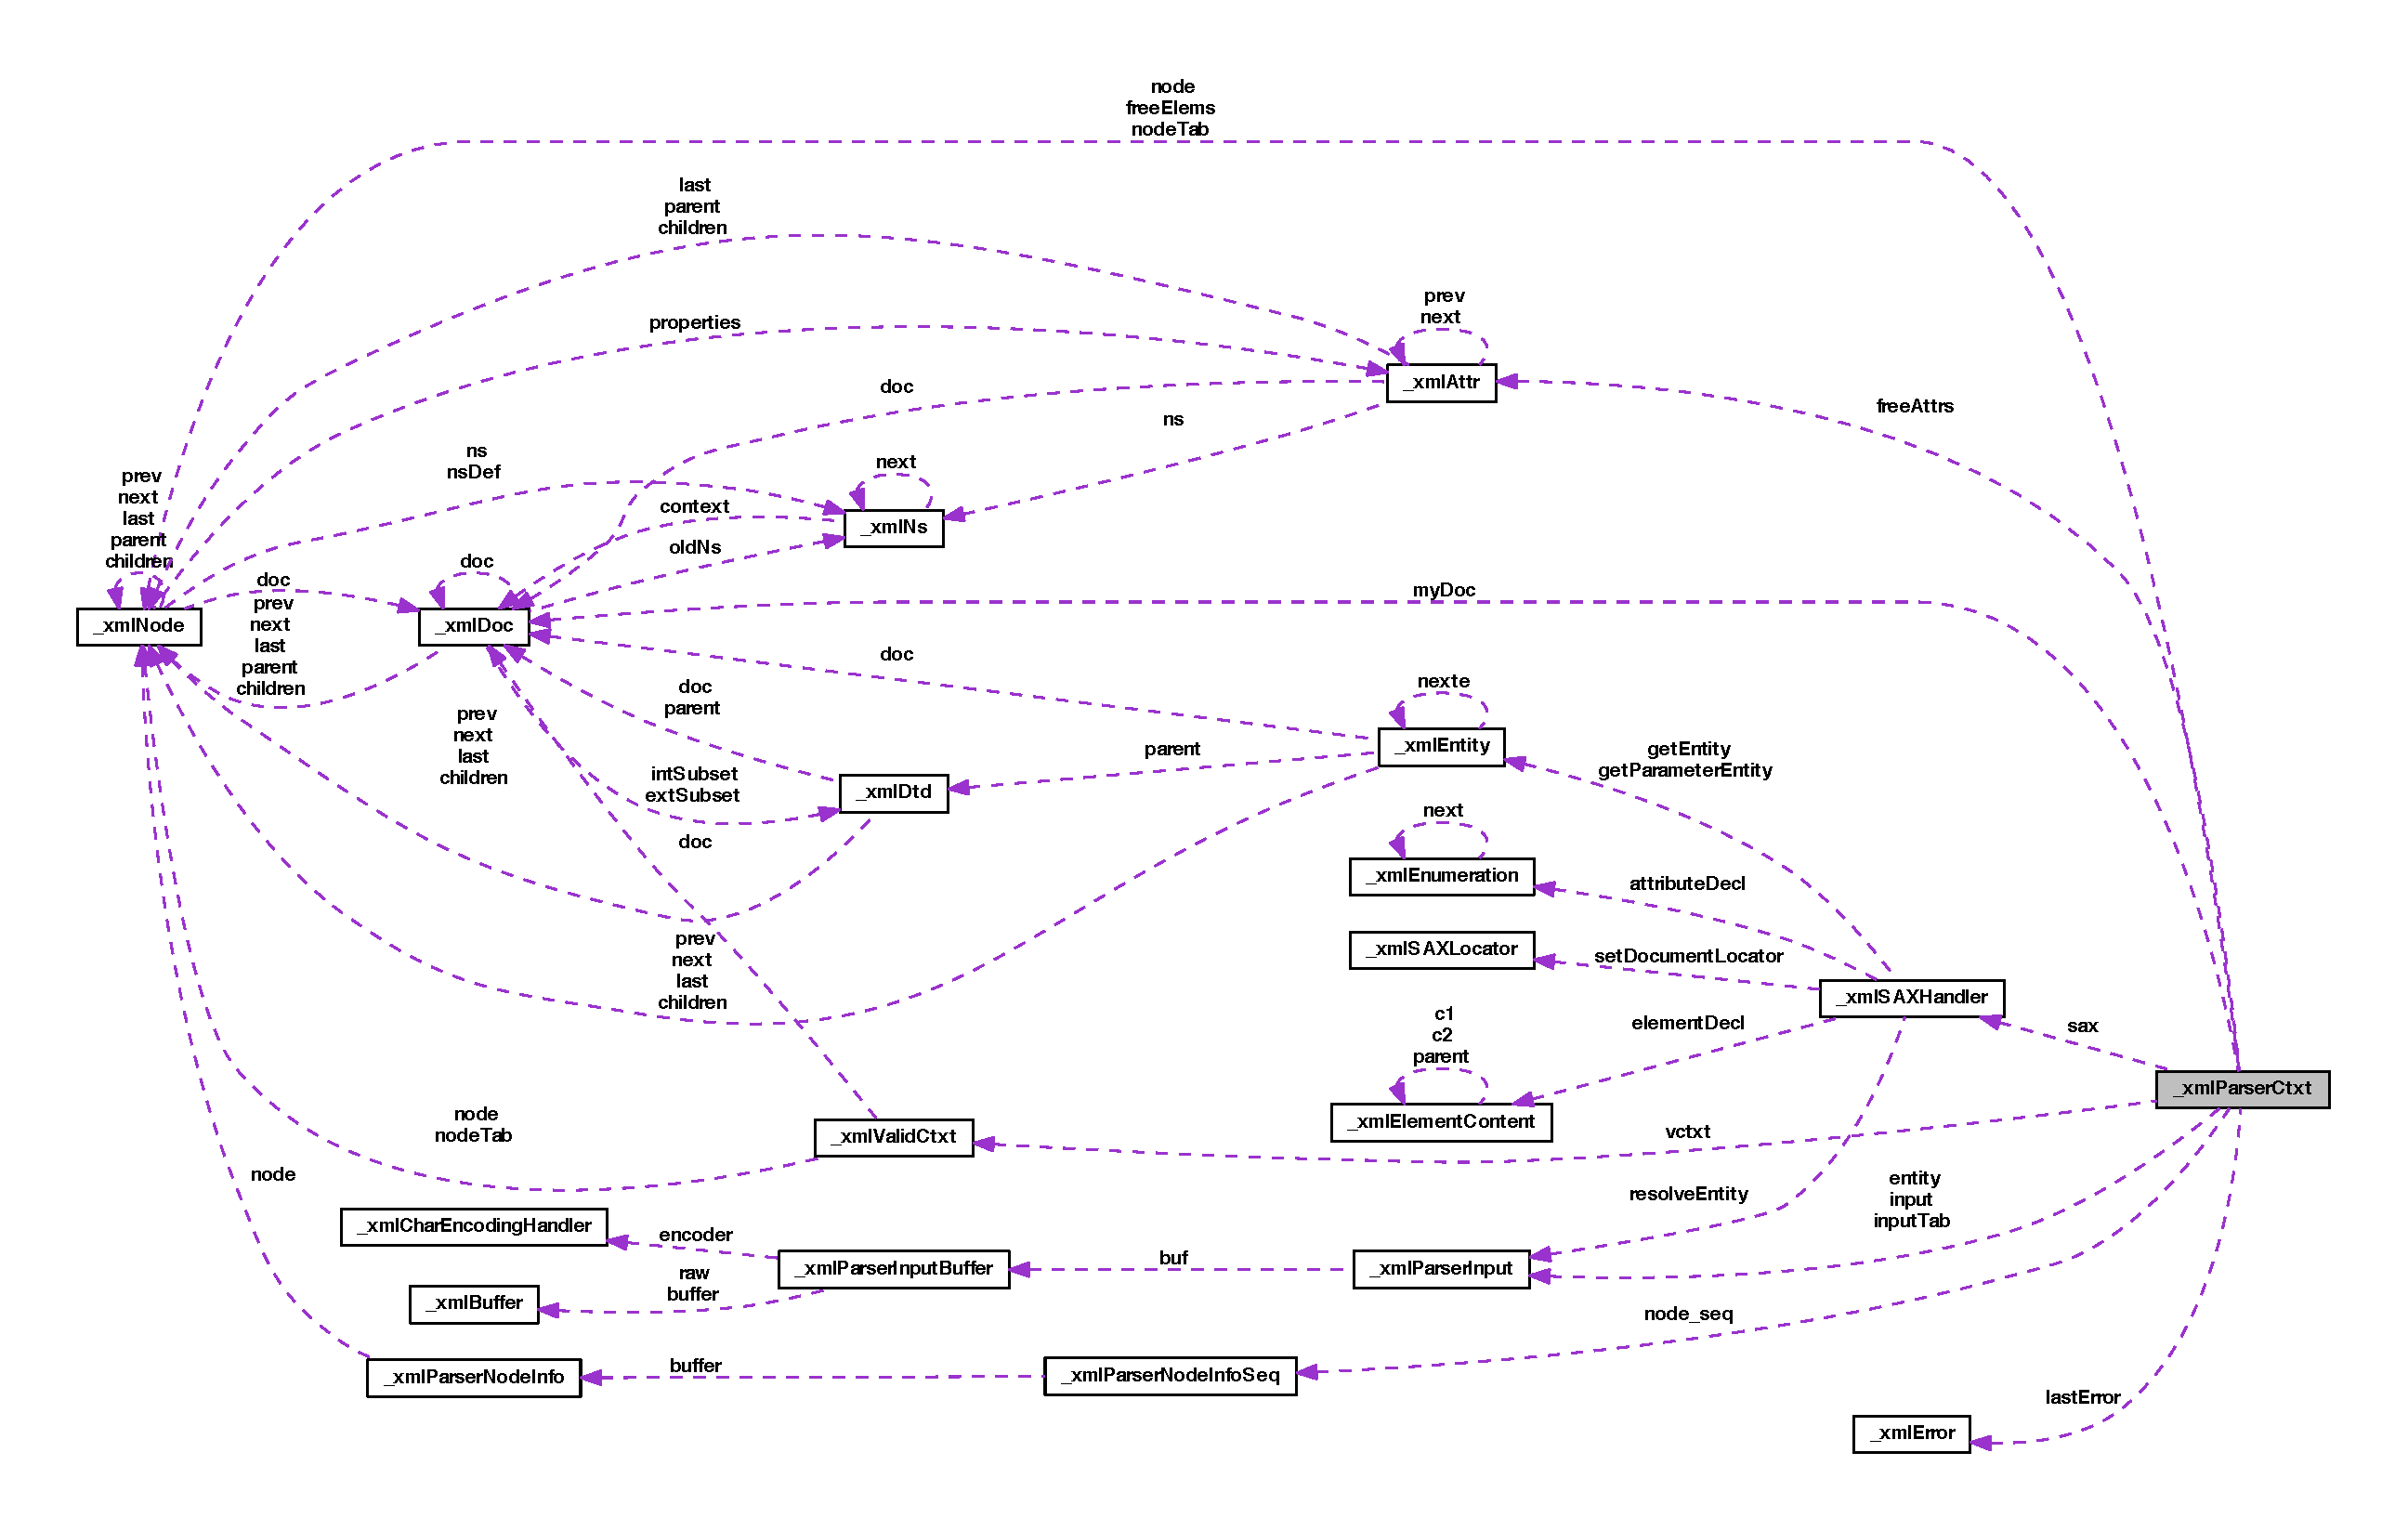
\includegraphics[width=350pt]{struct__xml_parser_ctxt__coll__graph}
\end{center}
\end{figure}
\subsection*{Public Attributes}
\begin{DoxyCompactItemize}
\item 
\hypertarget{struct__xml_parser_ctxt_aa1d637d91e6f2f1699e559c86f5a447a}{struct \hyperlink{struct__xml_s_a_x_handler}{\-\_\-xml\-S\-A\-X\-Handler} $\ast$ {\bfseries sax}}\label{struct__xml_parser_ctxt_aa1d637d91e6f2f1699e559c86f5a447a}

\item 
\hypertarget{struct__xml_parser_ctxt_a747f08df3539768575225645053f2ad4}{void $\ast$ {\bfseries user\-Data}}\label{struct__xml_parser_ctxt_a747f08df3539768575225645053f2ad4}

\item 
\hypertarget{struct__xml_parser_ctxt_a7058431b5a7781f3ecb400a0687b35de}{\hyperlink{struct__xml_doc}{xml\-Doc\-Ptr} {\bfseries my\-Doc}}\label{struct__xml_parser_ctxt_a7058431b5a7781f3ecb400a0687b35de}

\item 
\hypertarget{struct__xml_parser_ctxt_a304fdc65a808cab0e5057770375d1809}{int {\bfseries well\-Formed}}\label{struct__xml_parser_ctxt_a304fdc65a808cab0e5057770375d1809}

\item 
\hypertarget{struct__xml_parser_ctxt_a1649ee3fa54a9a0a666f82c5738faf80}{int {\bfseries replace\-Entities}}\label{struct__xml_parser_ctxt_a1649ee3fa54a9a0a666f82c5738faf80}

\item 
\hypertarget{struct__xml_parser_ctxt_a3f30fed85e18680824b1df86559f4b8b}{const xml\-Char $\ast$ {\bfseries version}}\label{struct__xml_parser_ctxt_a3f30fed85e18680824b1df86559f4b8b}

\item 
\hypertarget{struct__xml_parser_ctxt_a807731b8b0e04e280bd2e92b499ae0f6}{const xml\-Char $\ast$ {\bfseries encoding}}\label{struct__xml_parser_ctxt_a807731b8b0e04e280bd2e92b499ae0f6}

\item 
\hypertarget{struct__xml_parser_ctxt_ad92c2a15082cf72806f8b6499b12b4d5}{int {\bfseries standalone}}\label{struct__xml_parser_ctxt_ad92c2a15082cf72806f8b6499b12b4d5}

\item 
\hypertarget{struct__xml_parser_ctxt_aa963b0ce68afd948cd56a4ec1894c82d}{int {\bfseries html}}\label{struct__xml_parser_ctxt_aa963b0ce68afd948cd56a4ec1894c82d}

\item 
\hypertarget{struct__xml_parser_ctxt_af8206afddd8fa7a780e42a963049697b}{\hyperlink{struct__xml_parser_input}{xml\-Parser\-Input\-Ptr} {\bfseries input}}\label{struct__xml_parser_ctxt_af8206afddd8fa7a780e42a963049697b}

\item 
\hypertarget{struct__xml_parser_ctxt_a810ebc704f76c8aa8ea7990581159822}{int {\bfseries input\-Nr}}\label{struct__xml_parser_ctxt_a810ebc704f76c8aa8ea7990581159822}

\item 
\hypertarget{struct__xml_parser_ctxt_a048f19467718dab3a8a069cfac9e4dad}{int {\bfseries input\-Max}}\label{struct__xml_parser_ctxt_a048f19467718dab3a8a069cfac9e4dad}

\item 
\hypertarget{struct__xml_parser_ctxt_a72989fec54d6194d39b49564c0f0714a}{\hyperlink{struct__xml_parser_input}{xml\-Parser\-Input\-Ptr} $\ast$ {\bfseries input\-Tab}}\label{struct__xml_parser_ctxt_a72989fec54d6194d39b49564c0f0714a}

\item 
\hypertarget{struct__xml_parser_ctxt_aeec26cdcb168cb04b9c7d78f24559d41}{\hyperlink{struct__xml_node}{xml\-Node\-Ptr} {\bfseries node}}\label{struct__xml_parser_ctxt_aeec26cdcb168cb04b9c7d78f24559d41}

\item 
\hypertarget{struct__xml_parser_ctxt_a5bf7f999acdf8ca93eec2b284136c9ce}{int {\bfseries node\-Nr}}\label{struct__xml_parser_ctxt_a5bf7f999acdf8ca93eec2b284136c9ce}

\item 
\hypertarget{struct__xml_parser_ctxt_a45b85da2db53d7b44217e44fa36facfe}{int {\bfseries node\-Max}}\label{struct__xml_parser_ctxt_a45b85da2db53d7b44217e44fa36facfe}

\item 
\hypertarget{struct__xml_parser_ctxt_ab816108dd6a665ab67cdf5db97955dad}{\hyperlink{struct__xml_node}{xml\-Node\-Ptr} $\ast$ {\bfseries node\-Tab}}\label{struct__xml_parser_ctxt_ab816108dd6a665ab67cdf5db97955dad}

\item 
\hypertarget{struct__xml_parser_ctxt_ad25fd020c9638c8c83d1ca20e9c654d0}{int {\bfseries record\-\_\-info}}\label{struct__xml_parser_ctxt_ad25fd020c9638c8c83d1ca20e9c654d0}

\item 
\hypertarget{struct__xml_parser_ctxt_a67ea88a46d6f75ee30ea0ae1c5b231e1}{\hyperlink{struct__xml_parser_node_info_seq}{xml\-Parser\-Node\-Info\-Seq} {\bfseries node\-\_\-seq}}\label{struct__xml_parser_ctxt_a67ea88a46d6f75ee30ea0ae1c5b231e1}

\item 
\hypertarget{struct__xml_parser_ctxt_a18c6437841924c5d32203447e2bc09cf}{int {\bfseries err\-No}}\label{struct__xml_parser_ctxt_a18c6437841924c5d32203447e2bc09cf}

\item 
\hypertarget{struct__xml_parser_ctxt_a71dea0c007d91137762b6344501c6e76}{int {\bfseries has\-External\-Subset}}\label{struct__xml_parser_ctxt_a71dea0c007d91137762b6344501c6e76}

\item 
\hypertarget{struct__xml_parser_ctxt_a17eae9a89a2cc2a642a91b82848f18cb}{int {\bfseries has\-P\-Erefs}}\label{struct__xml_parser_ctxt_a17eae9a89a2cc2a642a91b82848f18cb}

\item 
\hypertarget{struct__xml_parser_ctxt_a28a2603f4c465b5ffb680ab32331ce63}{int {\bfseries external}}\label{struct__xml_parser_ctxt_a28a2603f4c465b5ffb680ab32331ce63}

\item 
\hypertarget{struct__xml_parser_ctxt_a45c179682750430ef82ef5ab5f362268}{int {\bfseries valid}}\label{struct__xml_parser_ctxt_a45c179682750430ef82ef5ab5f362268}

\item 
\hypertarget{struct__xml_parser_ctxt_af152215ec777654003b8c1303702b6d0}{int {\bfseries validate}}\label{struct__xml_parser_ctxt_af152215ec777654003b8c1303702b6d0}

\item 
\hypertarget{struct__xml_parser_ctxt_a19e33aa85d0096a58474ca1b8cc08bec}{xml\-Valid\-Ctxt {\bfseries vctxt}}\label{struct__xml_parser_ctxt_a19e33aa85d0096a58474ca1b8cc08bec}

\item 
\hypertarget{struct__xml_parser_ctxt_a7c245b95e3490e3f36777e591e212c09}{xml\-Parser\-Input\-State {\bfseries instate}}\label{struct__xml_parser_ctxt_a7c245b95e3490e3f36777e591e212c09}

\item 
\hypertarget{struct__xml_parser_ctxt_abfb170aa1cc309760fec4ab80c9d7fa5}{int {\bfseries token}}\label{struct__xml_parser_ctxt_abfb170aa1cc309760fec4ab80c9d7fa5}

\item 
\hypertarget{struct__xml_parser_ctxt_a5fc2c708d3e7aa7152edb9f80de2ea14}{char $\ast$ {\bfseries directory}}\label{struct__xml_parser_ctxt_a5fc2c708d3e7aa7152edb9f80de2ea14}

\item 
\hypertarget{struct__xml_parser_ctxt_a1380df2ee26fca1b223e9c8c4188f234}{const xml\-Char $\ast$ {\bfseries name}}\label{struct__xml_parser_ctxt_a1380df2ee26fca1b223e9c8c4188f234}

\item 
\hypertarget{struct__xml_parser_ctxt_a1b1150eb7811fb53c98e63e35d53e4b3}{int {\bfseries name\-Nr}}\label{struct__xml_parser_ctxt_a1b1150eb7811fb53c98e63e35d53e4b3}

\item 
\hypertarget{struct__xml_parser_ctxt_a6a0ab12d2cb34af65df75d7c2c583239}{int {\bfseries name\-Max}}\label{struct__xml_parser_ctxt_a6a0ab12d2cb34af65df75d7c2c583239}

\item 
\hypertarget{struct__xml_parser_ctxt_ab6543bd3266fbb270b97ce79d3cf6efa}{const xml\-Char $\ast$$\ast$ {\bfseries name\-Tab}}\label{struct__xml_parser_ctxt_ab6543bd3266fbb270b97ce79d3cf6efa}

\item 
\hypertarget{struct__xml_parser_ctxt_a4113f0fbbfd08c0f29cbc460cc86da79}{long {\bfseries nb\-Chars}}\label{struct__xml_parser_ctxt_a4113f0fbbfd08c0f29cbc460cc86da79}

\item 
\hypertarget{struct__xml_parser_ctxt_a74b3a4672d064ba4e2ef98d4c3e743db}{long {\bfseries check\-Index}}\label{struct__xml_parser_ctxt_a74b3a4672d064ba4e2ef98d4c3e743db}

\item 
\hypertarget{struct__xml_parser_ctxt_a1fa21b92fadb52c5b1b85a4916343671}{int {\bfseries keep\-Blanks}}\label{struct__xml_parser_ctxt_a1fa21b92fadb52c5b1b85a4916343671}

\item 
\hypertarget{struct__xml_parser_ctxt_a427c7da076659275c117e0697787dd48}{int {\bfseries disable\-S\-A\-X}}\label{struct__xml_parser_ctxt_a427c7da076659275c117e0697787dd48}

\item 
\hypertarget{struct__xml_parser_ctxt_ad63f2b246bc1550da0a7cf9987ee748c}{int {\bfseries in\-Subset}}\label{struct__xml_parser_ctxt_ad63f2b246bc1550da0a7cf9987ee748c}

\item 
\hypertarget{struct__xml_parser_ctxt_ae9d589b11d19abdfb137f50b3f4a88bc}{const xml\-Char $\ast$ {\bfseries int\-Sub\-Name}}\label{struct__xml_parser_ctxt_ae9d589b11d19abdfb137f50b3f4a88bc}

\item 
\hypertarget{struct__xml_parser_ctxt_a05cae3b71344fec07f7e20e9b685e653}{xml\-Char $\ast$ {\bfseries ext\-Sub\-U\-R\-I}}\label{struct__xml_parser_ctxt_a05cae3b71344fec07f7e20e9b685e653}

\item 
\hypertarget{struct__xml_parser_ctxt_aecb6a4ce823f6fccb60c8cba1f5cff68}{xml\-Char $\ast$ {\bfseries ext\-Sub\-System}}\label{struct__xml_parser_ctxt_aecb6a4ce823f6fccb60c8cba1f5cff68}

\item 
\hypertarget{struct__xml_parser_ctxt_a2002284f0a9dd3d435e6c6e7a31f7eb3}{int $\ast$ {\bfseries space}}\label{struct__xml_parser_ctxt_a2002284f0a9dd3d435e6c6e7a31f7eb3}

\item 
\hypertarget{struct__xml_parser_ctxt_ab8c1540b6c6e92500a302a94d6811c6c}{int {\bfseries space\-Nr}}\label{struct__xml_parser_ctxt_ab8c1540b6c6e92500a302a94d6811c6c}

\item 
\hypertarget{struct__xml_parser_ctxt_a2bf81df7c8f3436c87a74f84a2491a68}{int {\bfseries space\-Max}}\label{struct__xml_parser_ctxt_a2bf81df7c8f3436c87a74f84a2491a68}

\item 
\hypertarget{struct__xml_parser_ctxt_a0fabf85c9c305515f04dac83f47d52ba}{int $\ast$ {\bfseries space\-Tab}}\label{struct__xml_parser_ctxt_a0fabf85c9c305515f04dac83f47d52ba}

\item 
\hypertarget{struct__xml_parser_ctxt_a2a1d335b2cddf80f7a47733ab5c8d80f}{int {\bfseries depth}}\label{struct__xml_parser_ctxt_a2a1d335b2cddf80f7a47733ab5c8d80f}

\item 
\hypertarget{struct__xml_parser_ctxt_a512d34ee6ddbf6ce1f192757ae3a3ecf}{\hyperlink{struct__xml_parser_input}{xml\-Parser\-Input\-Ptr} {\bfseries entity}}\label{struct__xml_parser_ctxt_a512d34ee6ddbf6ce1f192757ae3a3ecf}

\item 
\hypertarget{struct__xml_parser_ctxt_af301648ace86f018fe05cb5dc3b6a102}{int {\bfseries charset}}\label{struct__xml_parser_ctxt_af301648ace86f018fe05cb5dc3b6a102}

\item 
\hypertarget{struct__xml_parser_ctxt_a30fec8f827d12f92cd0de13514cd889c}{int {\bfseries nodelen}}\label{struct__xml_parser_ctxt_a30fec8f827d12f92cd0de13514cd889c}

\item 
\hypertarget{struct__xml_parser_ctxt_a4eaca77096f011383a1c287f3d0fba15}{int {\bfseries nodemem}}\label{struct__xml_parser_ctxt_a4eaca77096f011383a1c287f3d0fba15}

\item 
\hypertarget{struct__xml_parser_ctxt_a796a6b0c9f0007e254efb062b93d1ae8}{int {\bfseries pedantic}}\label{struct__xml_parser_ctxt_a796a6b0c9f0007e254efb062b93d1ae8}

\item 
\hypertarget{struct__xml_parser_ctxt_a8735556c1156210bb0b97a02a1d8889d}{void $\ast$ {\bfseries \-\_\-private}}\label{struct__xml_parser_ctxt_a8735556c1156210bb0b97a02a1d8889d}

\item 
\hypertarget{struct__xml_parser_ctxt_a40da231797aa3b884594164515fb0324}{int {\bfseries loadsubset}}\label{struct__xml_parser_ctxt_a40da231797aa3b884594164515fb0324}

\item 
\hypertarget{struct__xml_parser_ctxt_aee2a9f6d1f92d0f418cf8e4a646f6015}{int {\bfseries linenumbers}}\label{struct__xml_parser_ctxt_aee2a9f6d1f92d0f418cf8e4a646f6015}

\item 
\hypertarget{struct__xml_parser_ctxt_a095521fb8cf11385de0783a0aefd03d8}{void $\ast$ {\bfseries catalogs}}\label{struct__xml_parser_ctxt_a095521fb8cf11385de0783a0aefd03d8}

\item 
\hypertarget{struct__xml_parser_ctxt_a9c51ae3fc1792162019746d718b87325}{int {\bfseries recovery}}\label{struct__xml_parser_ctxt_a9c51ae3fc1792162019746d718b87325}

\item 
\hypertarget{struct__xml_parser_ctxt_a3922f3d01fced1a3e0a9ed119617bc3b}{int {\bfseries progressive}}\label{struct__xml_parser_ctxt_a3922f3d01fced1a3e0a9ed119617bc3b}

\item 
\hypertarget{struct__xml_parser_ctxt_a9b94feda8017aa3343b4465254e73e6b}{xml\-Dict\-Ptr {\bfseries dict}}\label{struct__xml_parser_ctxt_a9b94feda8017aa3343b4465254e73e6b}

\item 
\hypertarget{struct__xml_parser_ctxt_a7196ecc0f6c93248bdc870938977dda0}{const xml\-Char $\ast$$\ast$ {\bfseries atts}}\label{struct__xml_parser_ctxt_a7196ecc0f6c93248bdc870938977dda0}

\item 
\hypertarget{struct__xml_parser_ctxt_a81b0f6978c0946d5f99cd8d08f33fb6f}{int {\bfseries maxatts}}\label{struct__xml_parser_ctxt_a81b0f6978c0946d5f99cd8d08f33fb6f}

\item 
\hypertarget{struct__xml_parser_ctxt_aceaa20243b828ee00343b8e9356d70a2}{int {\bfseries docdict}}\label{struct__xml_parser_ctxt_aceaa20243b828ee00343b8e9356d70a2}

\item 
\hypertarget{struct__xml_parser_ctxt_aa98063a5a3011d626d14d1a8bc68a7a1}{const xml\-Char $\ast$ {\bfseries str\-\_\-xml}}\label{struct__xml_parser_ctxt_aa98063a5a3011d626d14d1a8bc68a7a1}

\item 
\hypertarget{struct__xml_parser_ctxt_a1d16b1dbc896263601d0ac13786b13fe}{const xml\-Char $\ast$ {\bfseries str\-\_\-xmlns}}\label{struct__xml_parser_ctxt_a1d16b1dbc896263601d0ac13786b13fe}

\item 
\hypertarget{struct__xml_parser_ctxt_aa786dd994786980f18606f946b3ea79b}{const xml\-Char $\ast$ {\bfseries str\-\_\-xml\-\_\-ns}}\label{struct__xml_parser_ctxt_aa786dd994786980f18606f946b3ea79b}

\item 
\hypertarget{struct__xml_parser_ctxt_a6b8cc2efcfe76db0b97ba622d2eb9528}{int {\bfseries sax2}}\label{struct__xml_parser_ctxt_a6b8cc2efcfe76db0b97ba622d2eb9528}

\item 
\hypertarget{struct__xml_parser_ctxt_abea0de93d293184f4b128aa0a6c1086e}{int {\bfseries ns\-Nr}}\label{struct__xml_parser_ctxt_abea0de93d293184f4b128aa0a6c1086e}

\item 
\hypertarget{struct__xml_parser_ctxt_a8f66360c203d9a013575853da5d33914}{int {\bfseries ns\-Max}}\label{struct__xml_parser_ctxt_a8f66360c203d9a013575853da5d33914}

\item 
\hypertarget{struct__xml_parser_ctxt_a3ad86382cb5ade43536c753a3aa4ac20}{const xml\-Char $\ast$$\ast$ {\bfseries ns\-Tab}}\label{struct__xml_parser_ctxt_a3ad86382cb5ade43536c753a3aa4ac20}

\item 
\hypertarget{struct__xml_parser_ctxt_afba5a7515393e395795acbda236ac3c2}{int $\ast$ {\bfseries attallocs}}\label{struct__xml_parser_ctxt_afba5a7515393e395795acbda236ac3c2}

\item 
\hypertarget{struct__xml_parser_ctxt_a85198c5fd302d00678c9071ba1986952}{void $\ast$$\ast$ {\bfseries push\-Tab}}\label{struct__xml_parser_ctxt_a85198c5fd302d00678c9071ba1986952}

\item 
\hypertarget{struct__xml_parser_ctxt_ae6e54118b3c9a1d0b49163e5e8be50a5}{xml\-Hash\-Table\-Ptr {\bfseries atts\-Default}}\label{struct__xml_parser_ctxt_ae6e54118b3c9a1d0b49163e5e8be50a5}

\item 
\hypertarget{struct__xml_parser_ctxt_aa28f2a75723d92222abaea81ce3e94a8}{xml\-Hash\-Table\-Ptr {\bfseries atts\-Special}}\label{struct__xml_parser_ctxt_aa28f2a75723d92222abaea81ce3e94a8}

\item 
\hypertarget{struct__xml_parser_ctxt_a15f8e8be481f79a4636e643f72d464b0}{int {\bfseries ns\-Well\-Formed}}\label{struct__xml_parser_ctxt_a15f8e8be481f79a4636e643f72d464b0}

\item 
\hypertarget{struct__xml_parser_ctxt_a5f58199ceeb59e5faa1a6ea6d5a73502}{int {\bfseries options}}\label{struct__xml_parser_ctxt_a5f58199ceeb59e5faa1a6ea6d5a73502}

\item 
\hypertarget{struct__xml_parser_ctxt_a6e8ea51dd2f12067ebff135091cd97ed}{int {\bfseries dict\-Names}}\label{struct__xml_parser_ctxt_a6e8ea51dd2f12067ebff135091cd97ed}

\item 
\hypertarget{struct__xml_parser_ctxt_a47e2bf49432ad708a09298a8f441dbf3}{int {\bfseries free\-Elems\-Nr}}\label{struct__xml_parser_ctxt_a47e2bf49432ad708a09298a8f441dbf3}

\item 
\hypertarget{struct__xml_parser_ctxt_af6e6f367f0455e32cf2050fecf0f2647}{\hyperlink{struct__xml_node}{xml\-Node\-Ptr} {\bfseries free\-Elems}}\label{struct__xml_parser_ctxt_af6e6f367f0455e32cf2050fecf0f2647}

\item 
\hypertarget{struct__xml_parser_ctxt_a505367ee1fc8289be00afd4217a169be}{int {\bfseries free\-Attrs\-Nr}}\label{struct__xml_parser_ctxt_a505367ee1fc8289be00afd4217a169be}

\item 
\hypertarget{struct__xml_parser_ctxt_ac5c4d7b54b7e19da0256b7eacb5a159b}{\hyperlink{struct__xml_attr}{xml\-Attr\-Ptr} {\bfseries free\-Attrs}}\label{struct__xml_parser_ctxt_ac5c4d7b54b7e19da0256b7eacb5a159b}

\item 
\hypertarget{struct__xml_parser_ctxt_a06c58f3bc22c0d7c1ce76d607a5f44a9}{\hyperlink{struct__xml_error}{xml\-Error} {\bfseries last\-Error}}\label{struct__xml_parser_ctxt_a06c58f3bc22c0d7c1ce76d607a5f44a9}

\item 
\hypertarget{struct__xml_parser_ctxt_a000fedcc192734e86f5d4544b7ef12e1}{xml\-Parser\-Mode {\bfseries parse\-Mode}}\label{struct__xml_parser_ctxt_a000fedcc192734e86f5d4544b7ef12e1}

\end{DoxyCompactItemize}


\subsection{Detailed Description}
xml\-Parser\-Ctxt\-:

The parser context. N\-O\-T\-E This doesn't completely define the parser state, the (current ?) design of the parser uses recursive function calls since this allow and easy mapping from the production rules of the specification to the actual code. The drawback is that the actual function call also reflect the parser state. However most of the parsing routines takes as the only argument the parser context pointer, so migrating to a state based parser for progressive parsing shouldn't be too hard. 

Definition at line 184 of file parser.\-h.



The documentation for this struct was generated from the following files\-:\begin{DoxyCompactItemize}
\item 
Legiscode.\-applescript/build/\-Debug/\-Legiscode.\-applescript.\-app/\-Contents/\-Frameworks/libxml.\-framework/\-Versions/2.\-6.\-30/\-Headers/parser.\-h\item 
Legiscode.\-applescript/libxml.\-framework/\-Versions/2.\-6.\-30/\-Headers/parser.\-h\end{DoxyCompactItemize}

\hypertarget{struct__xml_parser_input}{\section{\-\_\-xml\-Parser\-Input Struct Reference}
\label{struct__xml_parser_input}\index{\-\_\-xml\-Parser\-Input@{\-\_\-xml\-Parser\-Input}}
}


Collaboration diagram for \-\_\-xml\-Parser\-Input\-:
\nopagebreak
\begin{figure}[H]
\begin{center}
\leavevmode
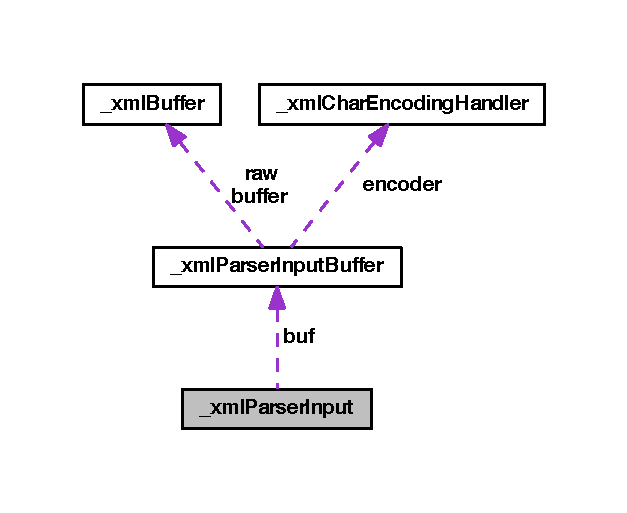
\includegraphics[width=301pt]{struct__xml_parser_input__coll__graph}
\end{center}
\end{figure}
\subsection*{Public Attributes}
\begin{DoxyCompactItemize}
\item 
\hypertarget{struct__xml_parser_input_ab50ed3b4b2f13d9c298d901395dfa531}{\hyperlink{struct__xml_parser_input_buffer}{xml\-Parser\-Input\-Buffer\-Ptr} {\bfseries buf}}\label{struct__xml_parser_input_ab50ed3b4b2f13d9c298d901395dfa531}

\item 
\hypertarget{struct__xml_parser_input_a8c84814dc9a4d5545dc5bd6a5bebf5e3}{const char $\ast$ {\bfseries filename}}\label{struct__xml_parser_input_a8c84814dc9a4d5545dc5bd6a5bebf5e3}

\item 
\hypertarget{struct__xml_parser_input_af7ab0de725e8086ef73ac8d12e61c1c9}{const char $\ast$ {\bfseries directory}}\label{struct__xml_parser_input_af7ab0de725e8086ef73ac8d12e61c1c9}

\item 
\hypertarget{struct__xml_parser_input_a19611a369c8af841f220210ad7d936b4}{const xml\-Char $\ast$ {\bfseries base}}\label{struct__xml_parser_input_a19611a369c8af841f220210ad7d936b4}

\item 
\hypertarget{struct__xml_parser_input_aba8f39b65dfcd6a2f8adc403d6cbf01b}{const xml\-Char $\ast$ {\bfseries cur}}\label{struct__xml_parser_input_aba8f39b65dfcd6a2f8adc403d6cbf01b}

\item 
\hypertarget{struct__xml_parser_input_a56257ad30a6806f118fa73db08c775fe}{const xml\-Char $\ast$ {\bfseries end}}\label{struct__xml_parser_input_a56257ad30a6806f118fa73db08c775fe}

\item 
\hypertarget{struct__xml_parser_input_a12d4752740620b43cc8fd64d13a7f91d}{int {\bfseries length}}\label{struct__xml_parser_input_a12d4752740620b43cc8fd64d13a7f91d}

\item 
\hypertarget{struct__xml_parser_input_a52689e7ee99ea4f70fea0da521371d43}{int {\bfseries line}}\label{struct__xml_parser_input_a52689e7ee99ea4f70fea0da521371d43}

\item 
\hypertarget{struct__xml_parser_input_a9be0a6d559062188aec7158b94cdde29}{int {\bfseries col}}\label{struct__xml_parser_input_a9be0a6d559062188aec7158b94cdde29}

\item 
\hypertarget{struct__xml_parser_input_aa4dbae4bbb1c3ffa212ad5d41402e587}{unsigned long {\bfseries consumed}}\label{struct__xml_parser_input_aa4dbae4bbb1c3ffa212ad5d41402e587}

\item 
\hypertarget{struct__xml_parser_input_a7c55373e42c374bc9df1c542274398fa}{xml\-Parser\-Input\-Deallocate {\bfseries free}}\label{struct__xml_parser_input_a7c55373e42c374bc9df1c542274398fa}

\item 
\hypertarget{struct__xml_parser_input_a5da2bb3d589073b7d472e6aa41ef4d81}{const xml\-Char $\ast$ {\bfseries encoding}}\label{struct__xml_parser_input_a5da2bb3d589073b7d472e6aa41ef4d81}

\item 
\hypertarget{struct__xml_parser_input_a83d340bb1a9cfacc2ac37ed0cc9d492d}{const xml\-Char $\ast$ {\bfseries version}}\label{struct__xml_parser_input_a83d340bb1a9cfacc2ac37ed0cc9d492d}

\item 
\hypertarget{struct__xml_parser_input_a2799e20f843ea79b753d9f8b60d4b793}{int {\bfseries standalone}}\label{struct__xml_parser_input_a2799e20f843ea79b753d9f8b60d4b793}

\item 
\hypertarget{struct__xml_parser_input_a20347691b442d481465e18f6777efecd}{int {\bfseries id}}\label{struct__xml_parser_input_a20347691b442d481465e18f6777efecd}

\end{DoxyCompactItemize}


\subsection{Detailed Description}


Definition at line 54 of file parser.\-h.



The documentation for this struct was generated from the following files\-:\begin{DoxyCompactItemize}
\item 
Legiscode.\-applescript/build/\-Debug/\-Legiscode.\-applescript.\-app/\-Contents/\-Frameworks/libxml.\-framework/\-Versions/2.\-6.\-30/\-Headers/parser.\-h\item 
Legiscode.\-applescript/libxml.\-framework/\-Versions/2.\-6.\-30/\-Headers/parser.\-h\end{DoxyCompactItemize}

\hypertarget{struct__xml_parser_input_buffer}{\section{\-\_\-xml\-Parser\-Input\-Buffer Struct Reference}
\label{struct__xml_parser_input_buffer}\index{\-\_\-xml\-Parser\-Input\-Buffer@{\-\_\-xml\-Parser\-Input\-Buffer}}
}


Collaboration diagram for \-\_\-xml\-Parser\-Input\-Buffer\-:
\nopagebreak
\begin{figure}[H]
\begin{center}
\leavevmode
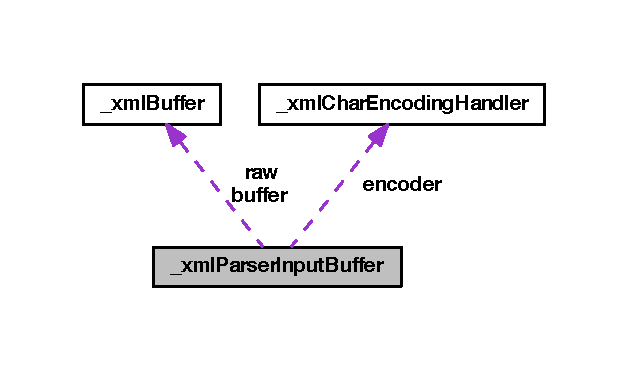
\includegraphics[width=301pt]{struct__xml_parser_input_buffer__coll__graph}
\end{center}
\end{figure}
\subsection*{Public Attributes}
\begin{DoxyCompactItemize}
\item 
\hypertarget{struct__xml_parser_input_buffer_afabe71b6b22a482e9a969053f04dbd36}{void $\ast$ {\bfseries context}}\label{struct__xml_parser_input_buffer_afabe71b6b22a482e9a969053f04dbd36}

\item 
\hypertarget{struct__xml_parser_input_buffer_a69f574b183e3acafcfb08e97370ca38a}{xml\-Input\-Read\-Callback {\bfseries readcallback}}\label{struct__xml_parser_input_buffer_a69f574b183e3acafcfb08e97370ca38a}

\item 
\hypertarget{struct__xml_parser_input_buffer_a2da9a3f7231857d19ac2ee41c61dfee2}{xml\-Input\-Close\-Callback {\bfseries closecallback}}\label{struct__xml_parser_input_buffer_a2da9a3f7231857d19ac2ee41c61dfee2}

\item 
\hypertarget{struct__xml_parser_input_buffer_af72974d4e9a48cdbd29c5071d07f3d69}{\hyperlink{struct__xml_char_encoding_handler}{xml\-Char\-Encoding\-Handler\-Ptr} {\bfseries encoder}}\label{struct__xml_parser_input_buffer_af72974d4e9a48cdbd29c5071d07f3d69}

\item 
\hypertarget{struct__xml_parser_input_buffer_acfa649a4c5dcaff889c49c885ea02af7}{\hyperlink{struct__xml_buffer}{xml\-Buffer\-Ptr} {\bfseries buffer}}\label{struct__xml_parser_input_buffer_acfa649a4c5dcaff889c49c885ea02af7}

\item 
\hypertarget{struct__xml_parser_input_buffer_a5a75f422c4d6a4d5a4c7da12b7564bfe}{\hyperlink{struct__xml_buffer}{xml\-Buffer\-Ptr} {\bfseries raw}}\label{struct__xml_parser_input_buffer_a5a75f422c4d6a4d5a4c7da12b7564bfe}

\item 
\hypertarget{struct__xml_parser_input_buffer_aa17c64fa46053ce3e42ac219d15418d4}{int {\bfseries compressed}}\label{struct__xml_parser_input_buffer_aa17c64fa46053ce3e42ac219d15418d4}

\item 
\hypertarget{struct__xml_parser_input_buffer_a5759b0b008b6fda05e9e850ed7bea149}{int {\bfseries error}}\label{struct__xml_parser_input_buffer_a5759b0b008b6fda05e9e850ed7bea149}

\item 
\hypertarget{struct__xml_parser_input_buffer_a1a63d0654d57e0d2a7ba52a06dc35b4a}{unsigned long {\bfseries rawconsumed}}\label{struct__xml_parser_input_buffer_a1a63d0654d57e0d2a7ba52a06dc35b4a}

\end{DoxyCompactItemize}


\subsection{Detailed Description}


Definition at line 125 of file xml\-I\-O.\-h.



The documentation for this struct was generated from the following files\-:\begin{DoxyCompactItemize}
\item 
Legiscode.\-applescript/build/\-Debug/\-Legiscode.\-applescript.\-app/\-Contents/\-Frameworks/libxml.\-framework/\-Versions/2.\-6.\-30/\-Headers/xml\-I\-O.\-h\item 
Legiscode.\-applescript/libxml.\-framework/\-Versions/2.\-6.\-30/\-Headers/xml\-I\-O.\-h\end{DoxyCompactItemize}

\input{struct__xml_parser_node_info}
\input{struct__xml_parser_node_info_seq}
\hypertarget{struct__xml_ref}{\section{\-\_\-xml\-Ref Struct Reference}
\label{struct__xml_ref}\index{\-\_\-xml\-Ref@{\-\_\-xml\-Ref}}
}


Collaboration diagram for \-\_\-xml\-Ref\-:
\nopagebreak
\begin{figure}[H]
\begin{center}
\leavevmode
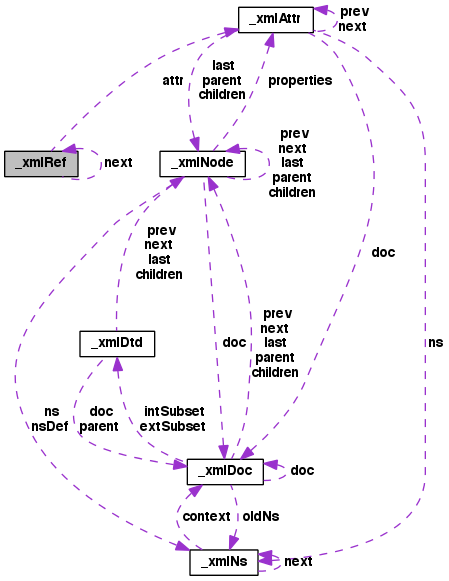
\includegraphics[width=350pt]{struct__xml_ref__coll__graph}
\end{center}
\end{figure}
\subsection*{Public Attributes}
\begin{DoxyCompactItemize}
\item 
\hypertarget{struct__xml_ref_a687313439b7753f7c2d42206e617ebdd}{struct \hyperlink{struct__xml_ref}{\-\_\-xml\-Ref} $\ast$ {\bfseries next}}\label{struct__xml_ref_a687313439b7753f7c2d42206e617ebdd}

\item 
\hypertarget{struct__xml_ref_a99f6334019561ed21376802349779d68}{const xml\-Char $\ast$ {\bfseries value}}\label{struct__xml_ref_a99f6334019561ed21376802349779d68}

\item 
\hypertarget{struct__xml_ref_a3ff97e4e127f1749ab2e59fdec0f8a8e}{\hyperlink{struct__xml_attr}{xml\-Attr\-Ptr} {\bfseries attr}}\label{struct__xml_ref_a3ff97e4e127f1749ab2e59fdec0f8a8e}

\item 
\hypertarget{struct__xml_ref_a6116f256b8edfa20d1ddc8cee7a320eb}{const xml\-Char $\ast$ {\bfseries name}}\label{struct__xml_ref_a6116f256b8edfa20d1ddc8cee7a320eb}

\item 
\hypertarget{struct__xml_ref_aa9d570e7f96cc7647c9b7fe96fc10eca}{int {\bfseries lineno}}\label{struct__xml_ref_aa9d570e7f96cc7647c9b7fe96fc10eca}

\end{DoxyCompactItemize}


\subsection{Detailed Description}


Definition at line 433 of file tree.\-h.



The documentation for this struct was generated from the following files\-:\begin{DoxyCompactItemize}
\item 
Legiscode.\-applescript/build/\-Debug/\-Legiscode.\-applescript.\-app/\-Contents/\-Frameworks/libxml.\-framework/\-Versions/2.\-6.\-30/\-Headers/tree.\-h\item 
Legiscode.\-applescript/libxml.\-framework/\-Versions/2.\-6.\-30/\-Headers/tree.\-h\end{DoxyCompactItemize}

\input{struct__xml_s_a_x_handler}
\hypertarget{struct__xml_s_a_x_handler_v1}{\section{\-\_\-xml\-S\-A\-X\-Handler\-V1 Struct Reference}
\label{struct__xml_s_a_x_handler_v1}\index{\-\_\-xml\-S\-A\-X\-Handler\-V1@{\-\_\-xml\-S\-A\-X\-Handler\-V1}}
}


Collaboration diagram for \-\_\-xml\-S\-A\-X\-Handler\-V1\-:
\nopagebreak
\begin{figure}[H]
\begin{center}
\leavevmode
\includegraphics[width=350pt]{struct__xml_s_a_x_handler_v1__coll__graph}
\end{center}
\end{figure}
\subsection*{Public Attributes}
\begin{DoxyCompactItemize}
\item 
\hypertarget{struct__xml_s_a_x_handler_v1_a42f4e20c793c236300b6101d49212580}{internal\-Subset\-S\-A\-X\-Func {\bfseries internal\-Subset}}\label{struct__xml_s_a_x_handler_v1_a42f4e20c793c236300b6101d49212580}

\item 
\hypertarget{struct__xml_s_a_x_handler_v1_a4b9bd1931ab440bd5b7d9df8009440bc}{is\-Standalone\-S\-A\-X\-Func {\bfseries is\-Standalone}}\label{struct__xml_s_a_x_handler_v1_a4b9bd1931ab440bd5b7d9df8009440bc}

\item 
\hypertarget{struct__xml_s_a_x_handler_v1_afe7c41e644a1152afd4bc13fe56a60de}{has\-Internal\-Subset\-S\-A\-X\-Func {\bfseries has\-Internal\-Subset}}\label{struct__xml_s_a_x_handler_v1_afe7c41e644a1152afd4bc13fe56a60de}

\item 
\hypertarget{struct__xml_s_a_x_handler_v1_a0ca8a76baf0d76b04d914ad9a56c4506}{has\-External\-Subset\-S\-A\-X\-Func {\bfseries has\-External\-Subset}}\label{struct__xml_s_a_x_handler_v1_a0ca8a76baf0d76b04d914ad9a56c4506}

\item 
\hypertarget{struct__xml_s_a_x_handler_v1_a949a9307787020339ed0d46376a676ea}{resolve\-Entity\-S\-A\-X\-Func {\bfseries resolve\-Entity}}\label{struct__xml_s_a_x_handler_v1_a949a9307787020339ed0d46376a676ea}

\item 
\hypertarget{struct__xml_s_a_x_handler_v1_a6d00cd90884aff134c70cfed77798cdb}{get\-Entity\-S\-A\-X\-Func {\bfseries get\-Entity}}\label{struct__xml_s_a_x_handler_v1_a6d00cd90884aff134c70cfed77798cdb}

\item 
\hypertarget{struct__xml_s_a_x_handler_v1_ab8767df981b572d1a4bb72de4eece794}{entity\-Decl\-S\-A\-X\-Func {\bfseries entity\-Decl}}\label{struct__xml_s_a_x_handler_v1_ab8767df981b572d1a4bb72de4eece794}

\item 
\hypertarget{struct__xml_s_a_x_handler_v1_a46b3e77687757223f11de89d19290e78}{notation\-Decl\-S\-A\-X\-Func {\bfseries notation\-Decl}}\label{struct__xml_s_a_x_handler_v1_a46b3e77687757223f11de89d19290e78}

\item 
\hypertarget{struct__xml_s_a_x_handler_v1_a0624527c2beaba134403534d02e4820f}{attribute\-Decl\-S\-A\-X\-Func {\bfseries attribute\-Decl}}\label{struct__xml_s_a_x_handler_v1_a0624527c2beaba134403534d02e4820f}

\item 
\hypertarget{struct__xml_s_a_x_handler_v1_a3248ebecb4a1b7eec246a535fe6bf08a}{element\-Decl\-S\-A\-X\-Func {\bfseries element\-Decl}}\label{struct__xml_s_a_x_handler_v1_a3248ebecb4a1b7eec246a535fe6bf08a}

\item 
\hypertarget{struct__xml_s_a_x_handler_v1_a91fa23c451584de06af7c0755e63e310}{unparsed\-Entity\-Decl\-S\-A\-X\-Func {\bfseries unparsed\-Entity\-Decl}}\label{struct__xml_s_a_x_handler_v1_a91fa23c451584de06af7c0755e63e310}

\item 
\hypertarget{struct__xml_s_a_x_handler_v1_ac607d4e2516d15e6ec10ea276ecdbfb2}{set\-Document\-Locator\-S\-A\-X\-Func {\bfseries set\-Document\-Locator}}\label{struct__xml_s_a_x_handler_v1_ac607d4e2516d15e6ec10ea276ecdbfb2}

\item 
\hypertarget{struct__xml_s_a_x_handler_v1_a1093326e92c519ef0298ab822933d2b1}{start\-Document\-S\-A\-X\-Func {\bfseries start\-Document}}\label{struct__xml_s_a_x_handler_v1_a1093326e92c519ef0298ab822933d2b1}

\item 
\hypertarget{struct__xml_s_a_x_handler_v1_a1cbd8f841c309cfc63973e75650a5aaf}{end\-Document\-S\-A\-X\-Func {\bfseries end\-Document}}\label{struct__xml_s_a_x_handler_v1_a1cbd8f841c309cfc63973e75650a5aaf}

\item 
\hypertarget{struct__xml_s_a_x_handler_v1_a311b1f74f2f6d0d167addfc49d39a435}{start\-Element\-S\-A\-X\-Func {\bfseries start\-Element}}\label{struct__xml_s_a_x_handler_v1_a311b1f74f2f6d0d167addfc49d39a435}

\item 
\hypertarget{struct__xml_s_a_x_handler_v1_ab62cf4d2df8209f439865179aaa641b9}{end\-Element\-S\-A\-X\-Func {\bfseries end\-Element}}\label{struct__xml_s_a_x_handler_v1_ab62cf4d2df8209f439865179aaa641b9}

\item 
\hypertarget{struct__xml_s_a_x_handler_v1_a88ed76850bc465258f158010f0c3c9be}{reference\-S\-A\-X\-Func {\bfseries reference}}\label{struct__xml_s_a_x_handler_v1_a88ed76850bc465258f158010f0c3c9be}

\item 
\hypertarget{struct__xml_s_a_x_handler_v1_a151b79b5c8ee8e05e10d69cb53953800}{characters\-S\-A\-X\-Func {\bfseries characters}}\label{struct__xml_s_a_x_handler_v1_a151b79b5c8ee8e05e10d69cb53953800}

\item 
\hypertarget{struct__xml_s_a_x_handler_v1_a0d25157139fc3e99e67f0a126dee5d5c}{ignorable\-Whitespace\-S\-A\-X\-Func {\bfseries ignorable\-Whitespace}}\label{struct__xml_s_a_x_handler_v1_a0d25157139fc3e99e67f0a126dee5d5c}

\item 
\hypertarget{struct__xml_s_a_x_handler_v1_a2d98ad46baa0f1a03ccca433e7541f65}{processing\-Instruction\-S\-A\-X\-Func {\bfseries processing\-Instruction}}\label{struct__xml_s_a_x_handler_v1_a2d98ad46baa0f1a03ccca433e7541f65}

\item 
\hypertarget{struct__xml_s_a_x_handler_v1_a0100dbc90526989b6ef1786d27253f3e}{comment\-S\-A\-X\-Func {\bfseries comment}}\label{struct__xml_s_a_x_handler_v1_a0100dbc90526989b6ef1786d27253f3e}

\item 
\hypertarget{struct__xml_s_a_x_handler_v1_abd9b23cf8beef529266afe74e9e82dbf}{warning\-S\-A\-X\-Func {\bfseries warning}}\label{struct__xml_s_a_x_handler_v1_abd9b23cf8beef529266afe74e9e82dbf}

\item 
\hypertarget{struct__xml_s_a_x_handler_v1_a944f9de403a5740bf219129523e49130}{error\-S\-A\-X\-Func {\bfseries error}}\label{struct__xml_s_a_x_handler_v1_a944f9de403a5740bf219129523e49130}

\item 
\hypertarget{struct__xml_s_a_x_handler_v1_a5b6797dbc24c30062a216c8d9da10ce8}{fatal\-Error\-S\-A\-X\-Func {\bfseries fatal\-Error}}\label{struct__xml_s_a_x_handler_v1_a5b6797dbc24c30062a216c8d9da10ce8}

\item 
\hypertarget{struct__xml_s_a_x_handler_v1_a3fa7627b54df41f9b7c4ffc56acf5093}{get\-Parameter\-Entity\-S\-A\-X\-Func {\bfseries get\-Parameter\-Entity}}\label{struct__xml_s_a_x_handler_v1_a3fa7627b54df41f9b7c4ffc56acf5093}

\item 
\hypertarget{struct__xml_s_a_x_handler_v1_a98acb685255099ea411bec6ba59aa3b1}{cdata\-Block\-S\-A\-X\-Func {\bfseries cdata\-Block}}\label{struct__xml_s_a_x_handler_v1_a98acb685255099ea411bec6ba59aa3b1}

\item 
\hypertarget{struct__xml_s_a_x_handler_v1_abed7b7b3c670bd6dceeffaf9ed7ea91d}{external\-Subset\-S\-A\-X\-Func {\bfseries external\-Subset}}\label{struct__xml_s_a_x_handler_v1_abed7b7b3c670bd6dceeffaf9ed7ea91d}

\item 
\hypertarget{struct__xml_s_a_x_handler_v1_aeed93655a47b1ea5c82a540b5843fa79}{unsigned int {\bfseries initialized}}\label{struct__xml_s_a_x_handler_v1_aeed93655a47b1ea5c82a540b5843fa79}

\end{DoxyCompactItemize}


\subsection{Detailed Description}


Definition at line 746 of file parser.\-h.



The documentation for this struct was generated from the following files\-:\begin{DoxyCompactItemize}
\item 
Legiscode.\-applescript/build/\-Debug/\-Legiscode.\-applescript.\-app/\-Contents/\-Frameworks/libxml.\-framework/\-Versions/2.\-6.\-30/\-Headers/parser.\-h\item 
Legiscode.\-applescript/libxml.\-framework/\-Versions/2.\-6.\-30/\-Headers/parser.\-h\end{DoxyCompactItemize}

\input{struct__xml_s_a_x_locator}
\hypertarget{struct__xml_u_r_i}{\section{\-\_\-xml\-U\-R\-I Struct Reference}
\label{struct__xml_u_r_i}\index{\-\_\-xml\-U\-R\-I@{\-\_\-xml\-U\-R\-I}}
}
\subsection*{Public Attributes}
\begin{DoxyCompactItemize}
\item 
\hypertarget{struct__xml_u_r_i_a98213a6dab42b0d5a3f8c87eed72acf4}{char $\ast$ {\bfseries scheme}}\label{struct__xml_u_r_i_a98213a6dab42b0d5a3f8c87eed72acf4}

\item 
\hypertarget{struct__xml_u_r_i_a335b3ef2183b31f15f51dd1b2c6241b9}{char $\ast$ {\bfseries opaque}}\label{struct__xml_u_r_i_a335b3ef2183b31f15f51dd1b2c6241b9}

\item 
\hypertarget{struct__xml_u_r_i_a9fc857bdd1702385e563977c2116fe95}{char $\ast$ {\bfseries authority}}\label{struct__xml_u_r_i_a9fc857bdd1702385e563977c2116fe95}

\item 
\hypertarget{struct__xml_u_r_i_a638c9f05ef24bf892d7a00ebf803b98a}{char $\ast$ {\bfseries server}}\label{struct__xml_u_r_i_a638c9f05ef24bf892d7a00ebf803b98a}

\item 
\hypertarget{struct__xml_u_r_i_ab620b70b2d63af398fc84281c4af421a}{char $\ast$ {\bfseries user}}\label{struct__xml_u_r_i_ab620b70b2d63af398fc84281c4af421a}

\item 
\hypertarget{struct__xml_u_r_i_a8460fd17316181c550e4f5b04e212eba}{int {\bfseries port}}\label{struct__xml_u_r_i_a8460fd17316181c550e4f5b04e212eba}

\item 
\hypertarget{struct__xml_u_r_i_ad592348964cebdf912086a3f3f8d686c}{char $\ast$ {\bfseries path}}\label{struct__xml_u_r_i_ad592348964cebdf912086a3f3f8d686c}

\item 
\hypertarget{struct__xml_u_r_i_ae7949d2e45af4b2fea60b3b51f6f991e}{char $\ast$ {\bfseries query}}\label{struct__xml_u_r_i_ae7949d2e45af4b2fea60b3b51f6f991e}

\item 
\hypertarget{struct__xml_u_r_i_ad9ebb4fe051996bba69c4db86836db7b}{char $\ast$ {\bfseries fragment}}\label{struct__xml_u_r_i_ad9ebb4fe051996bba69c4db86836db7b}

\item 
\hypertarget{struct__xml_u_r_i_a88f7bca5886e16c467eb1e1d4e729059}{int {\bfseries cleanup}}\label{struct__xml_u_r_i_a88f7bca5886e16c467eb1e1d4e729059}

\item 
\hypertarget{struct__xml_u_r_i_aad140cbc01f17eb488e4a798d91211e9}{char $\ast$ {\bfseries query\-\_\-raw}}\label{struct__xml_u_r_i_aad140cbc01f17eb488e4a798d91211e9}

\end{DoxyCompactItemize}


\subsection{Detailed Description}


Definition at line 33 of file uri.\-h.



The documentation for this struct was generated from the following files\-:\begin{DoxyCompactItemize}
\item 
Legiscode.\-applescript/build/\-Debug/\-Legiscode.\-applescript.\-app/\-Contents/\-Frameworks/libxml.\-framework/\-Versions/2.\-6.\-30/\-Headers/uri.\-h\item 
Legiscode.\-applescript/libxml.\-framework/\-Versions/2.\-6.\-30/\-Headers/uri.\-h\end{DoxyCompactItemize}

\hypertarget{struct__xml_valid_ctxt}{\section{\-\_\-xml\-Valid\-Ctxt Struct Reference}
\label{struct__xml_valid_ctxt}\index{\-\_\-xml\-Valid\-Ctxt@{\-\_\-xml\-Valid\-Ctxt}}
}


Collaboration diagram for \-\_\-xml\-Valid\-Ctxt\-:
\nopagebreak
\begin{figure}[H]
\begin{center}
\leavevmode
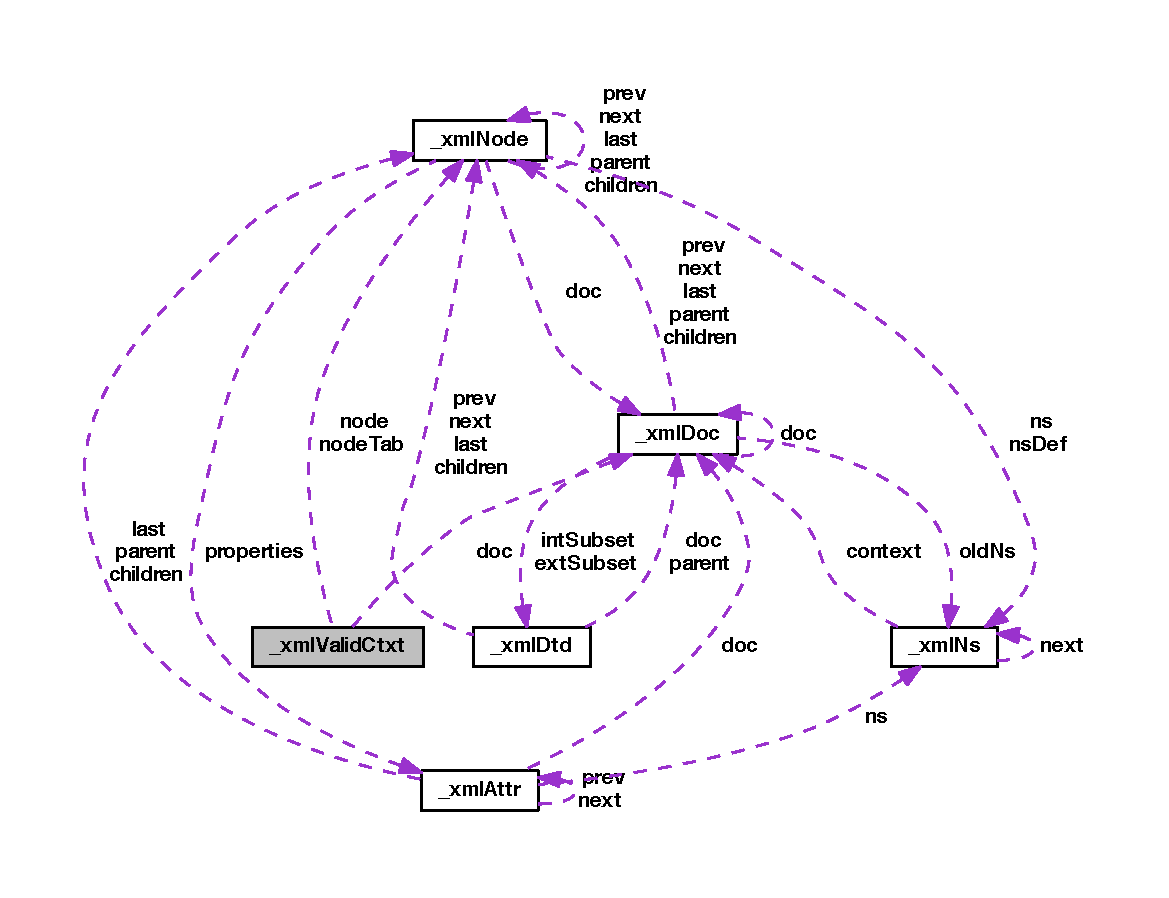
\includegraphics[width=350pt]{struct__xml_valid_ctxt__coll__graph}
\end{center}
\end{figure}
\subsection*{Public Attributes}
\begin{DoxyCompactItemize}
\item 
\hypertarget{struct__xml_valid_ctxt_ab57b3fe40347817a07d41cbc454cf6c1}{void $\ast$ {\bfseries user\-Data}}\label{struct__xml_valid_ctxt_ab57b3fe40347817a07d41cbc454cf6c1}

\item 
\hypertarget{struct__xml_valid_ctxt_a67cb1147c3d53a4cb2920987b091ff7a}{xml\-Validity\-Error\-Func {\bfseries error}}\label{struct__xml_valid_ctxt_a67cb1147c3d53a4cb2920987b091ff7a}

\item 
\hypertarget{struct__xml_valid_ctxt_af4ce21729ce719fd2c84e7c8d1f69413}{xml\-Validity\-Warning\-Func {\bfseries warning}}\label{struct__xml_valid_ctxt_af4ce21729ce719fd2c84e7c8d1f69413}

\item 
\hypertarget{struct__xml_valid_ctxt_a3b3eca74a3d7965394d7cda4974e673a}{\hyperlink{struct__xml_node}{xml\-Node\-Ptr} {\bfseries node}}\label{struct__xml_valid_ctxt_a3b3eca74a3d7965394d7cda4974e673a}

\item 
\hypertarget{struct__xml_valid_ctxt_a22247258390f6c2d960e26d915aa8bcb}{int {\bfseries node\-Nr}}\label{struct__xml_valid_ctxt_a22247258390f6c2d960e26d915aa8bcb}

\item 
\hypertarget{struct__xml_valid_ctxt_acb50c245f7c4afbdb5b5e6d56f108d97}{int {\bfseries node\-Max}}\label{struct__xml_valid_ctxt_acb50c245f7c4afbdb5b5e6d56f108d97}

\item 
\hypertarget{struct__xml_valid_ctxt_a2b8af03dea73d64bf9fcbacd7789f75d}{\hyperlink{struct__xml_node}{xml\-Node\-Ptr} $\ast$ {\bfseries node\-Tab}}\label{struct__xml_valid_ctxt_a2b8af03dea73d64bf9fcbacd7789f75d}

\item 
\hypertarget{struct__xml_valid_ctxt_a34ff820a3378c7742c09f6daeacd4db5}{unsigned int {\bfseries finish\-Dtd}}\label{struct__xml_valid_ctxt_a34ff820a3378c7742c09f6daeacd4db5}

\item 
\hypertarget{struct__xml_valid_ctxt_a1f084e858e3a50fa87696738c6d6a019}{\hyperlink{struct__xml_doc}{xml\-Doc\-Ptr} {\bfseries doc}}\label{struct__xml_valid_ctxt_a1f084e858e3a50fa87696738c6d6a019}

\item 
\hypertarget{struct__xml_valid_ctxt_ac31686aaeedb48c46b453f98c51597d2}{int {\bfseries valid}}\label{struct__xml_valid_ctxt_ac31686aaeedb48c46b453f98c51597d2}

\item 
\hypertarget{struct__xml_valid_ctxt_a505fa615ed796a0c19ae7aa138f59cdb}{xml\-Valid\-State $\ast$ {\bfseries vstate}}\label{struct__xml_valid_ctxt_a505fa615ed796a0c19ae7aa138f59cdb}

\item 
\hypertarget{struct__xml_valid_ctxt_af1d9fbfcf068c8dad6349fd677effc22}{int {\bfseries vstate\-Nr}}\label{struct__xml_valid_ctxt_af1d9fbfcf068c8dad6349fd677effc22}

\item 
\hypertarget{struct__xml_valid_ctxt_a606af121a4d33a9ec572147b17682125}{int {\bfseries vstate\-Max}}\label{struct__xml_valid_ctxt_a606af121a4d33a9ec572147b17682125}

\item 
\hypertarget{struct__xml_valid_ctxt_a91dd5e7865bb44737114e03a28bef3c2}{xml\-Valid\-State $\ast$ {\bfseries vstate\-Tab}}\label{struct__xml_valid_ctxt_a91dd5e7865bb44737114e03a28bef3c2}

\item 
\hypertarget{struct__xml_valid_ctxt_aa848a928c3edf586854a75e830700b83}{void $\ast$ {\bfseries am}}\label{struct__xml_valid_ctxt_aa848a928c3edf586854a75e830700b83}

\item 
\hypertarget{struct__xml_valid_ctxt_a1ddb6b8a2e152af3d6dbe5e5eb9e07d2}{void $\ast$ {\bfseries state}}\label{struct__xml_valid_ctxt_a1ddb6b8a2e152af3d6dbe5e5eb9e07d2}

\end{DoxyCompactItemize}


\subsection{Detailed Description}


Definition at line 82 of file valid.\-h.



The documentation for this struct was generated from the following files\-:\begin{DoxyCompactItemize}
\item 
Legiscode.\-applescript/build/\-Debug/\-Legiscode.\-applescript.\-app/\-Contents/\-Frameworks/libxml.\-framework/\-Versions/2.\-6.\-30/\-Headers/valid.\-h\item 
Legiscode.\-applescript/libxml.\-framework/\-Versions/2.\-6.\-30/\-Headers/valid.\-h\end{DoxyCompactItemize}

\input{struct_assignment_stmt_node}
\input{struct_block_node}
\input{struct_block_node_list}
\input{struct_cast_expr_node}
\hypertarget{struct_cast_stmt_node}{\section{Cast\-Stmt\-Node Struct Reference}
\label{struct_cast_stmt_node}\index{Cast\-Stmt\-Node@{Cast\-Stmt\-Node}}
}


{\ttfamily \#include $<$parser.\-h$>$}



Collaboration diagram for Cast\-Stmt\-Node\-:
\nopagebreak
\begin{figure}[H]
\begin{center}
\leavevmode
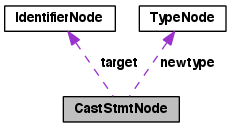
\includegraphics[width=245pt]{struct_cast_stmt_node__coll__graph}
\end{center}
\end{figure}
\subsection*{Public Attributes}
\begin{DoxyCompactItemize}
\item 
\hyperlink{struct_identifier_node}{Identifier\-Node} $\ast$ \hyperlink{struct_cast_stmt_node_a89d56358f0a8fc4d4fb0df7029ea494e}{target}
\item 
\hyperlink{struct_type_node}{Type\-Node} $\ast$ \hyperlink{struct_cast_stmt_node_adbeebc6cefa4f2cb92079b82cb4f4df8}{newtype}
\end{DoxyCompactItemize}


\subsection{Detailed Description}
Stores a cast statement. A cast statement changes the type of a variable identified by {\itshape target\/} to the type given by {\itshape newtype\/}.

\begin{DoxySeeAlso}{See also}
create\-Cast\-Stmt\-Node(\-Identifier\-Node $\ast$, Type\-Node $\ast$) 

delete\-Cast\-Stmt\-Node(\-Cast\-Stmt\-Node $\ast$) 
\end{DoxySeeAlso}


Definition at line 363 of file parser.\-h.



\subsection{Member Data Documentation}
\hypertarget{struct_cast_stmt_node_adbeebc6cefa4f2cb92079b82cb4f4df8}{\index{Cast\-Stmt\-Node@{Cast\-Stmt\-Node}!newtype@{newtype}}
\index{newtype@{newtype}!CastStmtNode@{Cast\-Stmt\-Node}}
\subsubsection[{newtype}]{\setlength{\rightskip}{0pt plus 5cm}{\bf Type\-Node}$\ast$ {\bf Cast\-Stmt\-Node\-::newtype}}}\label{struct_cast_stmt_node_adbeebc6cefa4f2cb92079b82cb4f4df8}
A pointer to the type to change {\itshape target\/} to. 

Definition at line 365 of file parser.\-h.

\hypertarget{struct_cast_stmt_node_a89d56358f0a8fc4d4fb0df7029ea494e}{\index{Cast\-Stmt\-Node@{Cast\-Stmt\-Node}!target@{target}}
\index{target@{target}!CastStmtNode@{Cast\-Stmt\-Node}}
\subsubsection[{target}]{\setlength{\rightskip}{0pt plus 5cm}{\bf Identifier\-Node}$\ast$ {\bf Cast\-Stmt\-Node\-::target}}}\label{struct_cast_stmt_node_a89d56358f0a8fc4d4fb0df7029ea494e}
A pointer to the name of the variable whose type is to be changed to {\itshape newtype\/}. 

Definition at line 364 of file parser.\-h.



The documentation for this struct was generated from the following file\-:\begin{DoxyCompactItemize}
\item 
tools/lci/lciframework/parser.\-h\end{DoxyCompactItemize}

\hypertarget{union_constant_data}{\section{Constant\-Data Union Reference}
\label{union_constant_data}\index{Constant\-Data@{Constant\-Data}}
}


{\ttfamily \#include $<$parser.\-h$>$}

\subsection*{Public Attributes}
\begin{DoxyCompactItemize}
\item 
int \hyperlink{union_constant_data_a2bd6e6fb99485a02c81794d2a3fc5a41}{i}
\item 
float \hyperlink{union_constant_data_a9c3282f50d2b4fb9752bb55fed6d1ed2}{f}
\item 
char $\ast$ \hyperlink{union_constant_data_aee1ab22b8dd076717f5de146f8939b46}{s}
\end{DoxyCompactItemize}


\subsection{Detailed Description}
Stores the data associated with a \hyperlink{struct_constant_node}{Constant\-Node} structure. 

Definition at line 298 of file parser.\-h.



\subsection{Member Data Documentation}
\hypertarget{union_constant_data_a9c3282f50d2b4fb9752bb55fed6d1ed2}{\index{Constant\-Data@{Constant\-Data}!f@{f}}
\index{f@{f}!ConstantData@{Constant\-Data}}
\subsubsection[{f}]{\setlength{\rightskip}{0pt plus 5cm}float {\bf Constant\-Data\-::f}}}\label{union_constant_data_a9c3282f50d2b4fb9752bb55fed6d1ed2}
Floating point data. 

Definition at line 300 of file parser.\-h.

\hypertarget{union_constant_data_a2bd6e6fb99485a02c81794d2a3fc5a41}{\index{Constant\-Data@{Constant\-Data}!i@{i}}
\index{i@{i}!ConstantData@{Constant\-Data}}
\subsubsection[{i}]{\setlength{\rightskip}{0pt plus 5cm}int {\bf Constant\-Data\-::i}}}\label{union_constant_data_a2bd6e6fb99485a02c81794d2a3fc5a41}
Integer data. 

Definition at line 299 of file parser.\-h.

\hypertarget{union_constant_data_aee1ab22b8dd076717f5de146f8939b46}{\index{Constant\-Data@{Constant\-Data}!s@{s}}
\index{s@{s}!ConstantData@{Constant\-Data}}
\subsubsection[{s}]{\setlength{\rightskip}{0pt plus 5cm}char$\ast$ {\bf Constant\-Data\-::s}}}\label{union_constant_data_aee1ab22b8dd076717f5de146f8939b46}
Character string data. 

Definition at line 301 of file parser.\-h.



The documentation for this union was generated from the following file\-:\begin{DoxyCompactItemize}
\item 
tools/lci/lciframework/parser.\-h\end{DoxyCompactItemize}

\hypertarget{struct_constant_node}{\section{Constant\-Node Struct Reference}
\label{struct_constant_node}\index{Constant\-Node@{Constant\-Node}}
}


{\ttfamily \#include $<$parser.\-h$>$}



Collaboration diagram for Constant\-Node\-:
\nopagebreak
\begin{figure}[H]
\begin{center}
\leavevmode
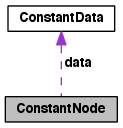
\includegraphics[width=164pt]{struct_constant_node__coll__graph}
\end{center}
\end{figure}
\subsection*{Public Attributes}
\begin{DoxyCompactItemize}
\item 
Constant\-Type \hyperlink{struct_constant_node_ae0c5b58398f2ff9a476628ea34858893}{type}
\item 
\hyperlink{union_constant_data}{Constant\-Data} \hyperlink{struct_constant_node_ae546bb49962906e06a965381014ea7ae}{data}
\end{DoxyCompactItemize}


\subsection{Detailed Description}
Stores a constant value. A constant value evaluates to its contents, depending on its {\itshape type\/}.

\begin{DoxySeeAlso}{See also}
create\-Boolean\-Constant\-Node(int) 

create\-Integer\-Constant\-Node(int) 

create\-Float\-Constant\-Node(float) 

create\-String\-Constant\-Node(char $\ast$) 

delete\-Constant\-Node(\-Constant\-Node $\ast$) 
\end{DoxySeeAlso}


Definition at line 312 of file parser.\-h.



\subsection{Member Data Documentation}
\hypertarget{struct_constant_node_ae546bb49962906e06a965381014ea7ae}{\index{Constant\-Node@{Constant\-Node}!data@{data}}
\index{data@{data}!ConstantNode@{Constant\-Node}}
\subsubsection[{data}]{\setlength{\rightskip}{0pt plus 5cm}{\bf Constant\-Data} {\bf Constant\-Node\-::data}}}\label{struct_constant_node_ae546bb49962906e06a965381014ea7ae}
The stored data of type {\itshape type\/}. 

Definition at line 314 of file parser.\-h.

\hypertarget{struct_constant_node_ae0c5b58398f2ff9a476628ea34858893}{\index{Constant\-Node@{Constant\-Node}!type@{type}}
\index{type@{type}!ConstantNode@{Constant\-Node}}
\subsubsection[{type}]{\setlength{\rightskip}{0pt plus 5cm}Constant\-Type {\bf Constant\-Node\-::type}}}\label{struct_constant_node_ae0c5b58398f2ff9a476628ea34858893}
The type of the constant. 

Definition at line 313 of file parser.\-h.



The documentation for this struct was generated from the following file\-:\begin{DoxyCompactItemize}
\item 
tools/lci/lciframework/parser.\-h\end{DoxyCompactItemize}

\hypertarget{struct_declaration_stmt_node}{\section{Declaration\-Stmt\-Node Struct Reference}
\label{struct_declaration_stmt_node}\index{Declaration\-Stmt\-Node@{Declaration\-Stmt\-Node}}
}


{\ttfamily \#include $<$parser.\-h$>$}



Collaboration diagram for Declaration\-Stmt\-Node\-:
\nopagebreak
\begin{figure}[H]
\begin{center}
\leavevmode
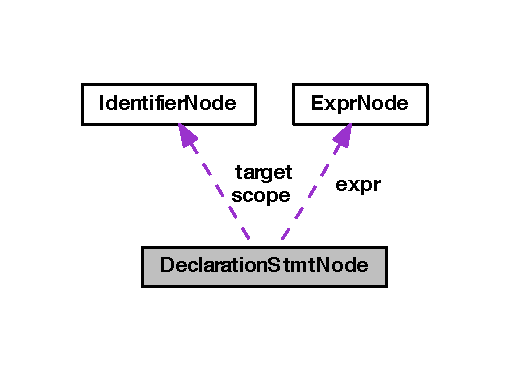
\includegraphics[width=245pt]{struct_declaration_stmt_node__coll__graph}
\end{center}
\end{figure}
\subsection*{Public Attributes}
\begin{DoxyCompactItemize}
\item 
\hyperlink{struct_identifier_node}{Identifier\-Node} $\ast$ \hyperlink{struct_declaration_stmt_node_ab52e3859c15ef8b651f330bcd963c56c}{scope}
\item 
\hyperlink{struct_identifier_node}{Identifier\-Node} $\ast$ \hyperlink{struct_declaration_stmt_node_a6fed156d07803ffd41487e873bcef98f}{target}
\item 
\hyperlink{struct_expr_node}{Expr\-Node} $\ast$ \hyperlink{struct_declaration_stmt_node_aba3f89fdd66c4b0264490aa639a6bd6f}{expr}
\end{DoxyCompactItemize}


\subsection{Detailed Description}
Stores a declaration statement. A declaration statement creates a new variable named by {\itshape target\/}, optionally initializing it to the evaluated contents of {\itshape expr\/}. {\itshape scope\/} determines which level of scope the variable is to be created in.

\begin{DoxySeeAlso}{See also}
create\-Declaration\-Stmt\-Node(\-Identifier\-Node $\ast$, Identifier\-Node $\ast$, Expr\-Node $\ast$) 

delete\-Declaration\-Stmt\-Node(\-Declaration\-Stmt\-Node $\ast$) 
\end{DoxySeeAlso}


Definition at line 405 of file parser.\-h.



\subsection{Member Data Documentation}
\hypertarget{struct_declaration_stmt_node_aba3f89fdd66c4b0264490aa639a6bd6f}{\index{Declaration\-Stmt\-Node@{Declaration\-Stmt\-Node}!expr@{expr}}
\index{expr@{expr}!DeclarationStmtNode@{Declaration\-Stmt\-Node}}
\subsubsection[{expr}]{\setlength{\rightskip}{0pt plus 5cm}{\bf Expr\-Node}$\ast$ {\bf Declaration\-Stmt\-Node\-::expr}}}\label{struct_declaration_stmt_node_aba3f89fdd66c4b0264490aa639a6bd6f}
An optional pointer to the expression to initialize {\itshape target\/} to. 

Definition at line 408 of file parser.\-h.

\hypertarget{struct_declaration_stmt_node_ab52e3859c15ef8b651f330bcd963c56c}{\index{Declaration\-Stmt\-Node@{Declaration\-Stmt\-Node}!scope@{scope}}
\index{scope@{scope}!DeclarationStmtNode@{Declaration\-Stmt\-Node}}
\subsubsection[{scope}]{\setlength{\rightskip}{0pt plus 5cm}{\bf Identifier\-Node}$\ast$ {\bf Declaration\-Stmt\-Node\-::scope}}}\label{struct_declaration_stmt_node_ab52e3859c15ef8b651f330bcd963c56c}
A pointer to the scope to create the variable in. 

Definition at line 406 of file parser.\-h.

\hypertarget{struct_declaration_stmt_node_a6fed156d07803ffd41487e873bcef98f}{\index{Declaration\-Stmt\-Node@{Declaration\-Stmt\-Node}!target@{target}}
\index{target@{target}!DeclarationStmtNode@{Declaration\-Stmt\-Node}}
\subsubsection[{target}]{\setlength{\rightskip}{0pt plus 5cm}{\bf Identifier\-Node}$\ast$ {\bf Declaration\-Stmt\-Node\-::target}}}\label{struct_declaration_stmt_node_a6fed156d07803ffd41487e873bcef98f}
A pointer to the name of the variable to create. 

Definition at line 407 of file parser.\-h.



The documentation for this struct was generated from the following file\-:\begin{DoxyCompactItemize}
\item 
tools/lci/lciframework/parser.\-h\end{DoxyCompactItemize}

\input{struct_expr_node}
\hypertarget{struct_expr_node_list}{\section{Expr\-Node\-List Struct Reference}
\label{struct_expr_node_list}\index{Expr\-Node\-List@{Expr\-Node\-List}}
}


{\ttfamily \#include $<$parser.\-h$>$}



Collaboration diagram for Expr\-Node\-List\-:
\nopagebreak
\begin{figure}[H]
\begin{center}
\leavevmode
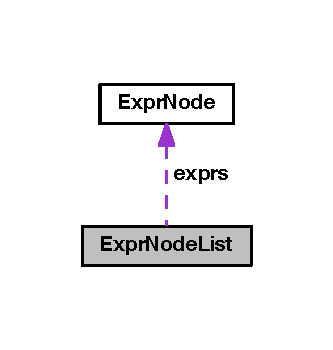
\includegraphics[width=160pt]{struct_expr_node_list__coll__graph}
\end{center}
\end{figure}
\subsection*{Public Attributes}
\begin{DoxyCompactItemize}
\item 
unsigned int \hyperlink{struct_expr_node_list_a60f9bbe230725287369033df733a2b04}{num}
\item 
\hyperlink{struct_expr_node}{Expr\-Node} $\ast$$\ast$ \hyperlink{struct_expr_node_list_a10ae95f2facec652ba79e0bb5c9298c1}{exprs}
\end{DoxyCompactItemize}


\subsection{Detailed Description}
Stores a list of expressions. This structure allows sets of expressions to be grouped together.

\begin{DoxySeeAlso}{See also}
create\-Expr\-Node\-List(void) 

add\-Expr\-Node(\-Expr\-Node\-List $\ast$, Expr\-Node $\ast$) 

delete\-Expr\-Node\-List(\-Expr\-Node\-List $\ast$) 
\end{DoxySeeAlso}


Definition at line 264 of file parser.\-h.



\subsection{Member Data Documentation}
\hypertarget{struct_expr_node_list_a10ae95f2facec652ba79e0bb5c9298c1}{\index{Expr\-Node\-List@{Expr\-Node\-List}!exprs@{exprs}}
\index{exprs@{exprs}!ExprNodeList@{Expr\-Node\-List}}
\subsubsection[{exprs}]{\setlength{\rightskip}{0pt plus 5cm}{\bf Expr\-Node}$\ast$$\ast$ {\bf Expr\-Node\-List\-::exprs}}}\label{struct_expr_node_list_a10ae95f2facec652ba79e0bb5c9298c1}
A pointer to an array of \hyperlink{struct_expr_node}{Expr\-Node} structures. 

Definition at line 266 of file parser.\-h.

\hypertarget{struct_expr_node_list_a60f9bbe230725287369033df733a2b04}{\index{Expr\-Node\-List@{Expr\-Node\-List}!num@{num}}
\index{num@{num}!ExprNodeList@{Expr\-Node\-List}}
\subsubsection[{num}]{\setlength{\rightskip}{0pt plus 5cm}unsigned int {\bf Expr\-Node\-List\-::num}}}\label{struct_expr_node_list_a60f9bbe230725287369033df733a2b04}
The number of \hyperlink{struct_expr_node}{Expr\-Node} structures stored. 

Definition at line 265 of file parser.\-h.



The documentation for this struct was generated from the following file\-:\begin{DoxyCompactItemize}
\item 
tools/lci/lciframework/parser.\-h\end{DoxyCompactItemize}

\input{struct_func_call_expr_node}
\hypertarget{struct_func_def_stmt_node}{\section{Func\-Def\-Stmt\-Node Struct Reference}
\label{struct_func_def_stmt_node}\index{Func\-Def\-Stmt\-Node@{Func\-Def\-Stmt\-Node}}
}


{\ttfamily \#include $<$parser.\-h$>$}



Collaboration diagram for Func\-Def\-Stmt\-Node\-:
\nopagebreak
\begin{figure}[H]
\begin{center}
\leavevmode
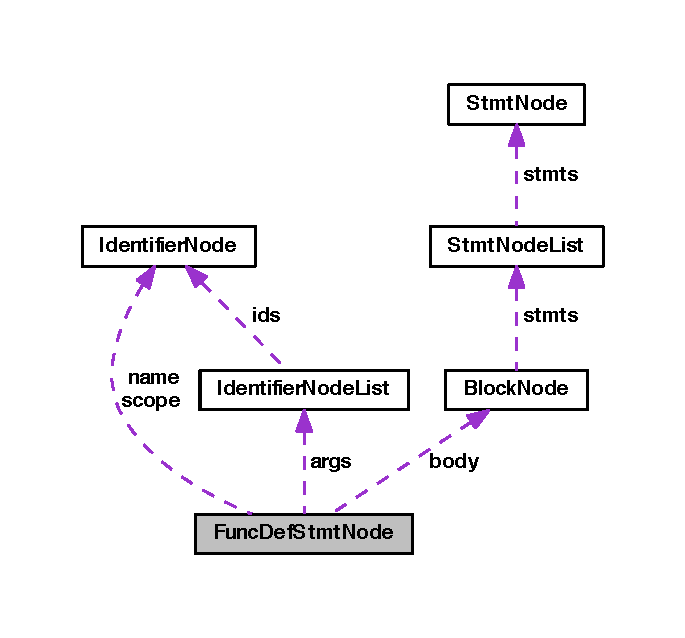
\includegraphics[width=329pt]{struct_func_def_stmt_node__coll__graph}
\end{center}
\end{figure}
\subsection*{Public Attributes}
\begin{DoxyCompactItemize}
\item 
\hyperlink{struct_identifier_node}{Identifier\-Node} $\ast$ \hyperlink{struct_func_def_stmt_node_a545e8a727dbe8786ab90afa0a4608d68}{scope}
\item 
\hyperlink{struct_identifier_node}{Identifier\-Node} $\ast$ \hyperlink{struct_func_def_stmt_node_ab047936127219724532e25ba6890265a}{name}
\item 
\hyperlink{struct_identifier_node_list}{Identifier\-Node\-List} $\ast$ \hyperlink{struct_func_def_stmt_node_a2a9f4d580b7252e5576873d2252a187a}{args}
\item 
\hyperlink{struct_block_node}{Block\-Node} $\ast$ \hyperlink{struct_func_def_stmt_node_a9e50b6a41f7abe43b433fe4fd714b002}{body}
\end{DoxyCompactItemize}


\subsection{Detailed Description}
Stores a function definition statement. A function definition statement defines the prototype and contents of a function.

\begin{DoxySeeAlso}{See also}
create\-Func\-Def\-Stmt\-Node(\-Identifier\-Node $\ast$, Identifier\-Node $\ast$, Identifier\-Node\-List $\ast$, Block\-Node $\ast$) 

delete\-Func\-Def\-Stmt\-Node(\-Func\-Def\-Stmt\-Node $\ast$) 
\end{DoxySeeAlso}


Definition at line 322 of file parser.\-h.



\subsection{Member Data Documentation}
\hypertarget{struct_func_def_stmt_node_a2a9f4d580b7252e5576873d2252a187a}{\index{Func\-Def\-Stmt\-Node@{Func\-Def\-Stmt\-Node}!args@{args}}
\index{args@{args}!FuncDefStmtNode@{Func\-Def\-Stmt\-Node}}
\subsubsection[{args}]{\setlength{\rightskip}{0pt plus 5cm}{\bf Identifier\-Node\-List}$\ast$ {\bf Func\-Def\-Stmt\-Node\-::args}}}\label{struct_func_def_stmt_node_a2a9f4d580b7252e5576873d2252a187a}
A pointer to a list of the names of the arguments of the function. 

Definition at line 325 of file parser.\-h.

\hypertarget{struct_func_def_stmt_node_a9e50b6a41f7abe43b433fe4fd714b002}{\index{Func\-Def\-Stmt\-Node@{Func\-Def\-Stmt\-Node}!body@{body}}
\index{body@{body}!FuncDefStmtNode@{Func\-Def\-Stmt\-Node}}
\subsubsection[{body}]{\setlength{\rightskip}{0pt plus 5cm}{\bf Block\-Node}$\ast$ {\bf Func\-Def\-Stmt\-Node\-::body}}}\label{struct_func_def_stmt_node_a9e50b6a41f7abe43b433fe4fd714b002}
A pointer to the block of code defined by the function. 

Definition at line 326 of file parser.\-h.

\hypertarget{struct_func_def_stmt_node_ab047936127219724532e25ba6890265a}{\index{Func\-Def\-Stmt\-Node@{Func\-Def\-Stmt\-Node}!name@{name}}
\index{name@{name}!FuncDefStmtNode@{Func\-Def\-Stmt\-Node}}
\subsubsection[{name}]{\setlength{\rightskip}{0pt plus 5cm}{\bf Identifier\-Node}$\ast$ {\bf Func\-Def\-Stmt\-Node\-::name}}}\label{struct_func_def_stmt_node_ab047936127219724532e25ba6890265a}
A pointer to the name of the function. 

Definition at line 324 of file parser.\-h.

\hypertarget{struct_func_def_stmt_node_a545e8a727dbe8786ab90afa0a4608d68}{\index{Func\-Def\-Stmt\-Node@{Func\-Def\-Stmt\-Node}!scope@{scope}}
\index{scope@{scope}!FuncDefStmtNode@{Func\-Def\-Stmt\-Node}}
\subsubsection[{scope}]{\setlength{\rightskip}{0pt plus 5cm}{\bf Identifier\-Node}$\ast$ {\bf Func\-Def\-Stmt\-Node\-::scope}}}\label{struct_func_def_stmt_node_a545e8a727dbe8786ab90afa0a4608d68}
A pointer to the scope to define the function in. 

Definition at line 323 of file parser.\-h.



The documentation for this struct was generated from the following file\-:\begin{DoxyCompactItemize}
\item 
tools/lci/lciframework/parser.\-h\end{DoxyCompactItemize}

\hypertarget{struct_function_table}{\section{Function\-Table Struct Reference}
\label{struct_function_table}\index{Function\-Table@{Function\-Table}}
}


{\ttfamily \#include $<$parser.\-h$>$}



Collaboration diagram for Function\-Table\-:
\nopagebreak
\begin{figure}[H]
\begin{center}
\leavevmode
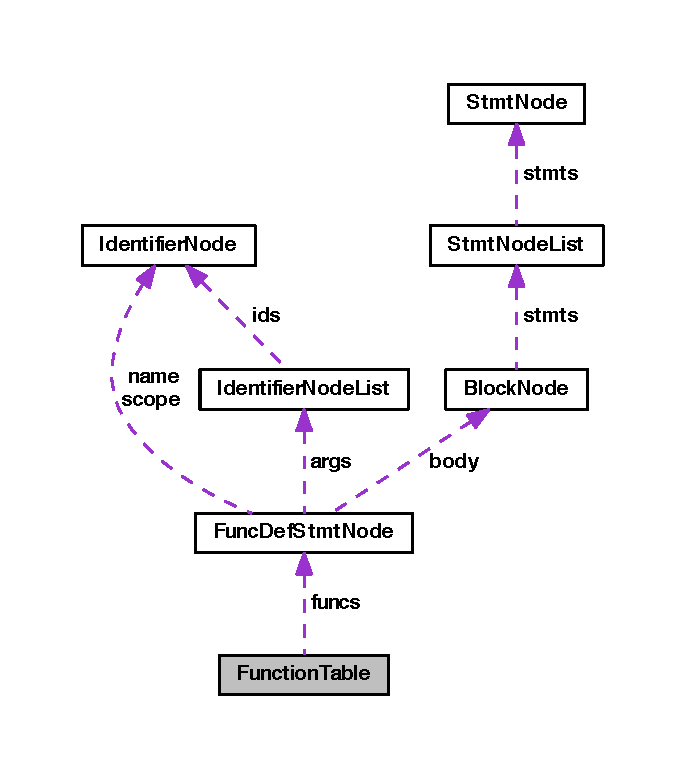
\includegraphics[width=329pt]{struct_function_table__coll__graph}
\end{center}
\end{figure}
\subsection*{Public Attributes}
\begin{DoxyCompactItemize}
\item 
unsigned int \hyperlink{struct_function_table_a568ae3641aaf56327da625e668c4aa51}{num}
\item 
\hyperlink{struct_func_def_stmt_node}{Func\-Def\-Stmt\-Node} $\ast$$\ast$ \hyperlink{struct_function_table_a1c1544bb6db2f638619e21fc60ca2ba8}{funcs}
\end{DoxyCompactItemize}


\subsection{Detailed Description}
Stores the contents of the function table. The function table contains the definitions of all declared functions. It is used for making sure function calls provide a valid arity, typechecking, however, is performed at runtime. 

Definition at line 333 of file parser.\-h.



\subsection{Member Data Documentation}
\hypertarget{struct_function_table_a1c1544bb6db2f638619e21fc60ca2ba8}{\index{Function\-Table@{Function\-Table}!funcs@{funcs}}
\index{funcs@{funcs}!FunctionTable@{Function\-Table}}
\subsubsection[{funcs}]{\setlength{\rightskip}{0pt plus 5cm}{\bf Func\-Def\-Stmt\-Node}$\ast$$\ast$ {\bf Function\-Table\-::funcs}}}\label{struct_function_table_a1c1544bb6db2f638619e21fc60ca2ba8}
A pointer to an array of declared functions. 

Definition at line 335 of file parser.\-h.

\hypertarget{struct_function_table_a568ae3641aaf56327da625e668c4aa51}{\index{Function\-Table@{Function\-Table}!num@{num}}
\index{num@{num}!FunctionTable@{Function\-Table}}
\subsubsection[{num}]{\setlength{\rightskip}{0pt plus 5cm}unsigned int {\bf Function\-Table\-::num}}}\label{struct_function_table_a568ae3641aaf56327da625e668c4aa51}
The number of declared functions. 

Definition at line 334 of file parser.\-h.



The documentation for this struct was generated from the following file\-:\begin{DoxyCompactItemize}
\item 
tools/lci/lciframework/parser.\-h\end{DoxyCompactItemize}

\input{struct_identifier_node}
\hypertarget{struct_identifier_node_list}{\section{Identifier\-Node\-List Struct Reference}
\label{struct_identifier_node_list}\index{Identifier\-Node\-List@{Identifier\-Node\-List}}
}


{\ttfamily \#include $<$parser.\-h$>$}



Collaboration diagram for Identifier\-Node\-List\-:
\nopagebreak
\begin{figure}[H]
\begin{center}
\leavevmode
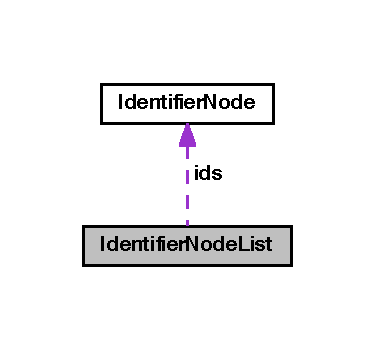
\includegraphics[width=180pt]{struct_identifier_node_list__coll__graph}
\end{center}
\end{figure}
\subsection*{Public Attributes}
\begin{DoxyCompactItemize}
\item 
unsigned int \hyperlink{struct_identifier_node_list_a7ee19db1c4e05eafe5df277542e01dd1}{num}
\item 
\hyperlink{struct_identifier_node}{Identifier\-Node} $\ast$$\ast$ \hyperlink{struct_identifier_node_list_a61b371619c07f89846ae0780d5403dc0}{ids}
\end{DoxyCompactItemize}


\subsection{Detailed Description}
Stores a list of identifiers. This structure allows sets of identifiers to be grouped together.

\begin{DoxySeeAlso}{See also}
create\-Identifier\-Node\-List(void) 

add\-Identifier\-Node(\-Identifier\-Node\-List $\ast$, Identifier\-Node $\ast$) 

delete\-Identifier\-Node\-List(\-Identifier\-Node\-List $\ast$) 
\end{DoxySeeAlso}


Definition at line 196 of file parser.\-h.



\subsection{Member Data Documentation}
\hypertarget{struct_identifier_node_list_a61b371619c07f89846ae0780d5403dc0}{\index{Identifier\-Node\-List@{Identifier\-Node\-List}!ids@{ids}}
\index{ids@{ids}!IdentifierNodeList@{Identifier\-Node\-List}}
\subsubsection[{ids}]{\setlength{\rightskip}{0pt plus 5cm}{\bf Identifier\-Node}$\ast$$\ast$ {\bf Identifier\-Node\-List\-::ids}}}\label{struct_identifier_node_list_a61b371619c07f89846ae0780d5403dc0}
A pointer to the array of \hyperlink{struct_identifier_node}{Identifier\-Node} structures. 

Definition at line 198 of file parser.\-h.

\hypertarget{struct_identifier_node_list_a7ee19db1c4e05eafe5df277542e01dd1}{\index{Identifier\-Node\-List@{Identifier\-Node\-List}!num@{num}}
\index{num@{num}!IdentifierNodeList@{Identifier\-Node\-List}}
\subsubsection[{num}]{\setlength{\rightskip}{0pt plus 5cm}unsigned int {\bf Identifier\-Node\-List\-::num}}}\label{struct_identifier_node_list_a7ee19db1c4e05eafe5df277542e01dd1}
The number of \hyperlink{struct_identifier_node}{Identifier\-Node} structures stored. 

Definition at line 197 of file parser.\-h.



The documentation for this struct was generated from the following file\-:\begin{DoxyCompactItemize}
\item 
tools/lci/lciframework/parser.\-h\end{DoxyCompactItemize}

\input{struct_if_then_else_stmt_node}
\hypertarget{struct_input_stmt_node}{\section{Input\-Stmt\-Node Struct Reference}
\label{struct_input_stmt_node}\index{Input\-Stmt\-Node@{Input\-Stmt\-Node}}
}


{\ttfamily \#include $<$parser.\-h$>$}



Collaboration diagram for Input\-Stmt\-Node\-:
\nopagebreak
\begin{figure}[H]
\begin{center}
\leavevmode
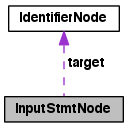
\includegraphics[width=168pt]{struct_input_stmt_node__coll__graph}
\end{center}
\end{figure}
\subsection*{Public Attributes}
\begin{DoxyCompactItemize}
\item 
\hyperlink{struct_identifier_node}{Identifier\-Node} $\ast$ \hyperlink{struct_input_stmt_node_ad7cb247683faf94a9da01d08055349f2}{target}
\end{DoxyCompactItemize}


\subsection{Detailed Description}
Stores an input statement. An input statement accepts a line of input from the use on an input device (by default standard input) and stores it in a variable.

\begin{DoxySeeAlso}{See also}
create\-Input\-Stmt\-Node(\-Identifier\-Node $\ast$) 

delete\-Input\-Stmt\-Node(\-Input\-Stmt\-Node $\ast$) 
\end{DoxySeeAlso}


Definition at line 384 of file parser.\-h.



\subsection{Member Data Documentation}
\hypertarget{struct_input_stmt_node_ad7cb247683faf94a9da01d08055349f2}{\index{Input\-Stmt\-Node@{Input\-Stmt\-Node}!target@{target}}
\index{target@{target}!InputStmtNode@{Input\-Stmt\-Node}}
\subsubsection[{target}]{\setlength{\rightskip}{0pt plus 5cm}{\bf Identifier\-Node}$\ast$ {\bf Input\-Stmt\-Node\-::target}}}\label{struct_input_stmt_node_ad7cb247683faf94a9da01d08055349f2}
A pointer to the name of the variable to store the input in. 

Definition at line 385 of file parser.\-h.



The documentation for this struct was generated from the following file\-:\begin{DoxyCompactItemize}
\item 
tools/lci/lciframework/parser.\-h\end{DoxyCompactItemize}

\input{struct_lexeme}
\hypertarget{struct_lexeme_list}{\section{Lexeme\-List Struct Reference}
\label{struct_lexeme_list}\index{Lexeme\-List@{Lexeme\-List}}
}


{\ttfamily \#include $<$lexer.\-h$>$}



Collaboration diagram for Lexeme\-List\-:
\nopagebreak
\begin{figure}[H]
\begin{center}
\leavevmode
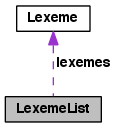
\includegraphics[width=159pt]{struct_lexeme_list__coll__graph}
\end{center}
\end{figure}
\subsection*{Public Attributes}
\begin{DoxyCompactItemize}
\item 
unsigned int \hyperlink{struct_lexeme_list_ab9e4971353dc5b435d604d3dbaef1857}{num}
\item 
\hyperlink{struct_lexeme}{Lexeme} $\ast$$\ast$ \hyperlink{struct_lexeme_list_a26e2c4bffe56f01e4d9b7c14ced653fd}{lexemes}
\end{DoxyCompactItemize}


\subsection{Detailed Description}
Stores a list of lexemes. This structure allows sets of lexemes to be grouped together.

\begin{DoxySeeAlso}{See also}
\hyperlink{lexer_8h_a03a7275accd6e39d369c689760bd15df}{create\-Lexeme\-List(void)} 

\hyperlink{lexer_8h_af9ec30b004772b01fb38f6dc4f54d102}{add\-Lexeme(\-Lexeme\-List $\ast$, Lexeme $\ast$)} 

\hyperlink{lexer_8h_a3a834cd76633550e9b8be7368cdeae3d}{delete\-Lexeme\-List(\-Lexeme\-List $\ast$)} 
\end{DoxySeeAlso}


Definition at line 43 of file lexer.\-h.



\subsection{Member Data Documentation}
\hypertarget{struct_lexeme_list_a26e2c4bffe56f01e4d9b7c14ced653fd}{\index{Lexeme\-List@{Lexeme\-List}!lexemes@{lexemes}}
\index{lexemes@{lexemes}!LexemeList@{Lexeme\-List}}
\subsubsection[{lexemes}]{\setlength{\rightskip}{0pt plus 5cm}{\bf Lexeme}$\ast$$\ast$ {\bf Lexeme\-List\-::lexemes}}}\label{struct_lexeme_list_a26e2c4bffe56f01e4d9b7c14ced653fd}
A pointer to the array of \hyperlink{struct_lexeme}{Lexeme} structures. 

Definition at line 45 of file lexer.\-h.

\hypertarget{struct_lexeme_list_ab9e4971353dc5b435d604d3dbaef1857}{\index{Lexeme\-List@{Lexeme\-List}!num@{num}}
\index{num@{num}!LexemeList@{Lexeme\-List}}
\subsubsection[{num}]{\setlength{\rightskip}{0pt plus 5cm}unsigned int {\bf Lexeme\-List\-::num}}}\label{struct_lexeme_list_ab9e4971353dc5b435d604d3dbaef1857}
The number of \hyperlink{struct_lexeme}{Lexeme} structures stored. 

Definition at line 44 of file lexer.\-h.



The documentation for this struct was generated from the following file\-:\begin{DoxyCompactItemize}
\item 
tools/lci/lciframework/\hyperlink{lexer_8h}{lexer.\-h}\end{DoxyCompactItemize}

\hypertarget{struct_loop_stmt_node}{\section{Loop\-Stmt\-Node Struct Reference}
\label{struct_loop_stmt_node}\index{Loop\-Stmt\-Node@{Loop\-Stmt\-Node}}
}


{\ttfamily \#include $<$parser.\-h$>$}



Collaboration diagram for Loop\-Stmt\-Node\-:
\nopagebreak
\begin{figure}[H]
\begin{center}
\leavevmode
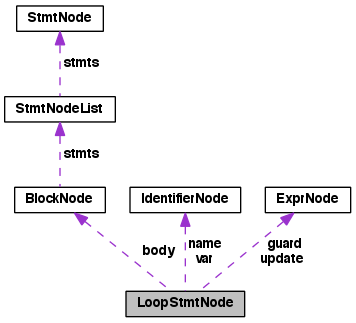
\includegraphics[width=339pt]{struct_loop_stmt_node__coll__graph}
\end{center}
\end{figure}
\subsection*{Public Attributes}
\begin{DoxyCompactItemize}
\item 
\hyperlink{struct_identifier_node}{Identifier\-Node} $\ast$ \hyperlink{struct_loop_stmt_node_a36b401d6c4fd2c16a68de026b99187f3}{name}
\item 
\hyperlink{struct_identifier_node}{Identifier\-Node} $\ast$ \hyperlink{struct_loop_stmt_node_afb3820072966231fd1d43eea8ebd9234}{var}
\item 
\hyperlink{struct_expr_node}{Expr\-Node} $\ast$ \hyperlink{struct_loop_stmt_node_a53a86fb7f989cf43f54192b8f3ad6c1a}{guard}
\item 
\hyperlink{struct_expr_node}{Expr\-Node} $\ast$ \hyperlink{struct_loop_stmt_node_a0400ab555fff51b09f79c495af20f37f}{update}
\item 
\hyperlink{struct_block_node}{Block\-Node} $\ast$ \hyperlink{struct_loop_stmt_node_a6844fd9206ed5d6b4fd48fc1365969aa}{body}
\end{DoxyCompactItemize}


\subsection{Detailed Description}
Stores a loop statement. A loop statement repeatedly executes its {\itshape body\/} while {\itshape guard\/} evaluates to true, executing {\itshape update\/} at the end of each cycle.

\begin{DoxySeeAlso}{See also}
create\-Loop\-Stmt\-Node(\-Identifier\-Node $\ast$, Identifier\-Node $\ast$, Expr\-Node $\ast$, Expr\-Node $\ast$, Block\-Node $\ast$) 

delete\-Loop\-Stmt\-Node(\-Loop\-Stmt\-Node $\ast$) 
\end{DoxySeeAlso}


Definition at line 457 of file parser.\-h.



\subsection{Member Data Documentation}
\hypertarget{struct_loop_stmt_node_a6844fd9206ed5d6b4fd48fc1365969aa}{\index{Loop\-Stmt\-Node@{Loop\-Stmt\-Node}!body@{body}}
\index{body@{body}!LoopStmtNode@{Loop\-Stmt\-Node}}
\subsubsection[{body}]{\setlength{\rightskip}{0pt plus 5cm}{\bf Block\-Node}$\ast$ {\bf Loop\-Stmt\-Node\-::body}}}\label{struct_loop_stmt_node_a6844fd9206ed5d6b4fd48fc1365969aa}
A pointer to the block of code to be executed with each iteration of the loop. 

Definition at line 462 of file parser.\-h.

\hypertarget{struct_loop_stmt_node_a53a86fb7f989cf43f54192b8f3ad6c1a}{\index{Loop\-Stmt\-Node@{Loop\-Stmt\-Node}!guard@{guard}}
\index{guard@{guard}!LoopStmtNode@{Loop\-Stmt\-Node}}
\subsubsection[{guard}]{\setlength{\rightskip}{0pt plus 5cm}{\bf Expr\-Node}$\ast$ {\bf Loop\-Stmt\-Node\-::guard}}}\label{struct_loop_stmt_node_a53a86fb7f989cf43f54192b8f3ad6c1a}
A pointer to the expression to determine if the loop will continue. 

Definition at line 460 of file parser.\-h.

\hypertarget{struct_loop_stmt_node_a36b401d6c4fd2c16a68de026b99187f3}{\index{Loop\-Stmt\-Node@{Loop\-Stmt\-Node}!name@{name}}
\index{name@{name}!LoopStmtNode@{Loop\-Stmt\-Node}}
\subsubsection[{name}]{\setlength{\rightskip}{0pt plus 5cm}{\bf Identifier\-Node}$\ast$ {\bf Loop\-Stmt\-Node\-::name}}}\label{struct_loop_stmt_node_a36b401d6c4fd2c16a68de026b99187f3}
A pointer to the name of the loop. 

Definition at line 458 of file parser.\-h.

\hypertarget{struct_loop_stmt_node_a0400ab555fff51b09f79c495af20f37f}{\index{Loop\-Stmt\-Node@{Loop\-Stmt\-Node}!update@{update}}
\index{update@{update}!LoopStmtNode@{Loop\-Stmt\-Node}}
\subsubsection[{update}]{\setlength{\rightskip}{0pt plus 5cm}{\bf Expr\-Node}$\ast$ {\bf Loop\-Stmt\-Node\-::update}}}\label{struct_loop_stmt_node_a0400ab555fff51b09f79c495af20f37f}
A pointer to the expression to evaluate to update {\itshape var\/}. 

Definition at line 461 of file parser.\-h.

\hypertarget{struct_loop_stmt_node_afb3820072966231fd1d43eea8ebd9234}{\index{Loop\-Stmt\-Node@{Loop\-Stmt\-Node}!var@{var}}
\index{var@{var}!LoopStmtNode@{Loop\-Stmt\-Node}}
\subsubsection[{var}]{\setlength{\rightskip}{0pt plus 5cm}{\bf Identifier\-Node}$\ast$ {\bf Loop\-Stmt\-Node\-::var}}}\label{struct_loop_stmt_node_afb3820072966231fd1d43eea8ebd9234}
A pointer to the name of the variable to be updated by {\itshape update\/}. 

Definition at line 459 of file parser.\-h.



The documentation for this struct was generated from the following file\-:\begin{DoxyCompactItemize}
\item 
tools/lci/lciframework/parser.\-h\end{DoxyCompactItemize}

\hypertarget{struct_main_node}{\section{Main\-Node Struct Reference}
\label{struct_main_node}\index{Main\-Node@{Main\-Node}}
}


{\ttfamily \#include $<$parser.\-h$>$}



Collaboration diagram for Main\-Node\-:
\nopagebreak
\begin{figure}[H]
\begin{center}
\leavevmode
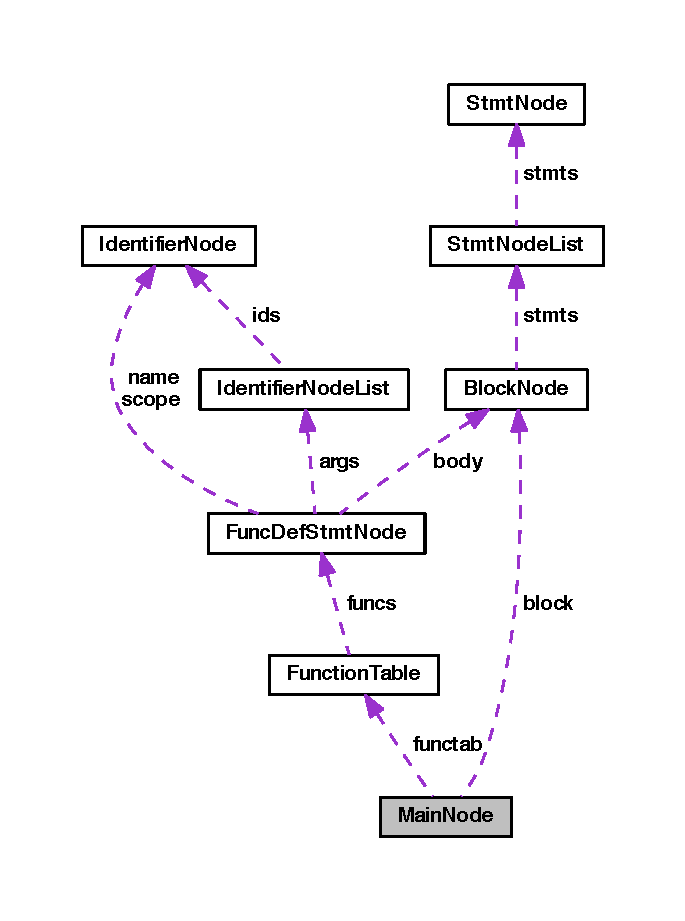
\includegraphics[width=329pt]{struct_main_node__coll__graph}
\end{center}
\end{figure}
\subsection*{Public Attributes}
\begin{DoxyCompactItemize}
\item 
\hyperlink{struct_block_node}{Block\-Node} $\ast$ \hyperlink{struct_main_node_aee302d107abb16c48702c2699a58d49f}{block}
\item 
\hyperlink{struct_function_table}{Function\-Table} $\ast$ \hyperlink{struct_main_node_a1b22e4833219bb71c9ca7f32d3e37241}{functab}
\end{DoxyCompactItemize}


\subsection{Detailed Description}
Stores the main block of code a program executes. This structure could be accomplished using only a \hyperlink{struct_block_node}{Block\-Node} instead, but its logical importance to program control flow (namely, it is the first portion of code executed) merits its own structure.

\begin{DoxySeeAlso}{See also}
create\-Main\-Node(\-Block\-Node $\ast$) 

delete\-Main\-Node(\-Main\-Node $\ast$) 
\end{DoxySeeAlso}


Definition at line 345 of file parser.\-h.



\subsection{Member Data Documentation}
\hypertarget{struct_main_node_aee302d107abb16c48702c2699a58d49f}{\index{Main\-Node@{Main\-Node}!block@{block}}
\index{block@{block}!MainNode@{Main\-Node}}
\subsubsection[{block}]{\setlength{\rightskip}{0pt plus 5cm}{\bf Block\-Node}$\ast$ {\bf Main\-Node\-::block}}}\label{struct_main_node_aee302d107abb16c48702c2699a58d49f}
A pointer to the block of code to execute first. 

Definition at line 346 of file parser.\-h.

\hypertarget{struct_main_node_a1b22e4833219bb71c9ca7f32d3e37241}{\index{Main\-Node@{Main\-Node}!functab@{functab}}
\index{functab@{functab}!MainNode@{Main\-Node}}
\subsubsection[{functab}]{\setlength{\rightskip}{0pt plus 5cm}{\bf Function\-Table}$\ast$ {\bf Main\-Node\-::functab}}}\label{struct_main_node_a1b22e4833219bb71c9ca7f32d3e37241}
A pointer to the function table associated with this block of code. 

Definition at line 347 of file parser.\-h.



The documentation for this struct was generated from the following file\-:\begin{DoxyCompactItemize}
\item 
tools/lci/lciframework/parser.\-h\end{DoxyCompactItemize}

\input{interface_n_s_array_07_regex_kit_additions_08}
\hypertarget{interface_n_s_data_07_regex_kit_additions_08}{\section{N\-S\-Data(Regex\-Kit\-Additions) Class Reference}
\label{interface_n_s_data_07_regex_kit_additions_08}\index{N\-S\-Data(\-Regex\-Kit\-Additions)@{N\-S\-Data(\-Regex\-Kit\-Additions)}}
}
\subsection*{Public Member Functions}
\begin{DoxyCompactItemize}
\item 
\hypertarget{interface_n_s_data_07_regex_kit_additions_08_af8d3f7997646aab0cb78a11a06191777}{(B\-O\-O\-L) -\/ {\bfseries is\-Matched\-By\-Regex\-:}}\label{interface_n_s_data_07_regex_kit_additions_08_af8d3f7997646aab0cb78a11a06191777}

\item 
\hypertarget{interface_n_s_data_07_regex_kit_additions_08_a4ad7703b83285ba6e9679d78f98df9c9}{(B\-O\-O\-L) -\/ {\bfseries is\-Matched\-By\-Regex\-:in\-Range\-:}}\label{interface_n_s_data_07_regex_kit_additions_08_a4ad7703b83285ba6e9679d78f98df9c9}

\item 
\hypertarget{interface_n_s_data_07_regex_kit_additions_08_a79d7b1e74ce410450beb79b0e9fe1648}{(N\-S\-Range) -\/ {\bfseries range\-Of\-Regex\-:}}\label{interface_n_s_data_07_regex_kit_additions_08_a79d7b1e74ce410450beb79b0e9fe1648}

\item 
\hypertarget{interface_n_s_data_07_regex_kit_additions_08_a93352fef20624e15c6e0e8d358f8df21}{(N\-S\-Range) -\/ {\bfseries range\-Of\-Regex\-:in\-Range\-:capture\-:}}\label{interface_n_s_data_07_regex_kit_additions_08_a93352fef20624e15c6e0e8d358f8df21}

\item 
\hypertarget{interface_n_s_data_07_regex_kit_additions_08_afb09f7d4d30ad6871e975dbd574afbb2}{(N\-S\-Range $\ast$) -\/ {\bfseries ranges\-Of\-Regex\-:}}\label{interface_n_s_data_07_regex_kit_additions_08_afb09f7d4d30ad6871e975dbd574afbb2}

\item 
\hypertarget{interface_n_s_data_07_regex_kit_additions_08_a0b5438c8c31de2fceb1c32c529983d50}{(N\-S\-Range $\ast$) -\/ {\bfseries ranges\-Of\-Regex\-:in\-Range\-:}}\label{interface_n_s_data_07_regex_kit_additions_08_a0b5438c8c31de2fceb1c32c529983d50}

\item 
\hypertarget{interface_n_s_data_07_regex_kit_additions_08_acb6b0049863f670669e1fd604932c0a6}{(N\-S\-Data $\ast$) -\/ {\bfseries subdata\-By\-Matching\-:}}\label{interface_n_s_data_07_regex_kit_additions_08_acb6b0049863f670669e1fd604932c0a6}

\item 
\hypertarget{interface_n_s_data_07_regex_kit_additions_08_ad48af4d0814356cbe42d22b3c6782628}{(N\-S\-Data $\ast$) -\/ {\bfseries subdata\-By\-Matching\-:in\-Range\-:}}\label{interface_n_s_data_07_regex_kit_additions_08_ad48af4d0814356cbe42d22b3c6782628}

\item 
\hypertarget{interface_n_s_data_07_regex_kit_additions_08_af8d3f7997646aab0cb78a11a06191777}{(B\-O\-O\-L) -\/ {\bfseries is\-Matched\-By\-Regex\-:}}\label{interface_n_s_data_07_regex_kit_additions_08_af8d3f7997646aab0cb78a11a06191777}

\item 
\hypertarget{interface_n_s_data_07_regex_kit_additions_08_a4ad7703b83285ba6e9679d78f98df9c9}{(B\-O\-O\-L) -\/ {\bfseries is\-Matched\-By\-Regex\-:in\-Range\-:}}\label{interface_n_s_data_07_regex_kit_additions_08_a4ad7703b83285ba6e9679d78f98df9c9}

\item 
\hypertarget{interface_n_s_data_07_regex_kit_additions_08_a79d7b1e74ce410450beb79b0e9fe1648}{(N\-S\-Range) -\/ {\bfseries range\-Of\-Regex\-:}}\label{interface_n_s_data_07_regex_kit_additions_08_a79d7b1e74ce410450beb79b0e9fe1648}

\item 
\hypertarget{interface_n_s_data_07_regex_kit_additions_08_a93352fef20624e15c6e0e8d358f8df21}{(N\-S\-Range) -\/ {\bfseries range\-Of\-Regex\-:in\-Range\-:capture\-:}}\label{interface_n_s_data_07_regex_kit_additions_08_a93352fef20624e15c6e0e8d358f8df21}

\item 
\hypertarget{interface_n_s_data_07_regex_kit_additions_08_afb09f7d4d30ad6871e975dbd574afbb2}{(N\-S\-Range $\ast$) -\/ {\bfseries ranges\-Of\-Regex\-:}}\label{interface_n_s_data_07_regex_kit_additions_08_afb09f7d4d30ad6871e975dbd574afbb2}

\item 
\hypertarget{interface_n_s_data_07_regex_kit_additions_08_a0b5438c8c31de2fceb1c32c529983d50}{(N\-S\-Range $\ast$) -\/ {\bfseries ranges\-Of\-Regex\-:in\-Range\-:}}\label{interface_n_s_data_07_regex_kit_additions_08_a0b5438c8c31de2fceb1c32c529983d50}

\item 
\hypertarget{interface_n_s_data_07_regex_kit_additions_08_acb6b0049863f670669e1fd604932c0a6}{(N\-S\-Data $\ast$) -\/ {\bfseries subdata\-By\-Matching\-:}}\label{interface_n_s_data_07_regex_kit_additions_08_acb6b0049863f670669e1fd604932c0a6}

\item 
\hypertarget{interface_n_s_data_07_regex_kit_additions_08_ad48af4d0814356cbe42d22b3c6782628}{(N\-S\-Data $\ast$) -\/ {\bfseries subdata\-By\-Matching\-:in\-Range\-:}}\label{interface_n_s_data_07_regex_kit_additions_08_ad48af4d0814356cbe42d22b3c6782628}

\end{DoxyCompactItemize}


\subsection{Detailed Description}


Definition at line 50 of file N\-S\-Data.\-h.



The documentation for this class was generated from the following files\-:\begin{DoxyCompactItemize}
\item 
Legiscode.\-applescript/build/\-Debug/\-Legiscode.\-applescript.\-app/\-Contents/\-Frameworks/\-Regex\-Kit.\-framework/\-Versions/\-A/\-Headers/N\-S\-Data.\-h\item 
Legiscode.\-applescript/\-Regex\-Kit.\-framework/\-Versions/\-A/\-Headers/N\-S\-Data.\-h\end{DoxyCompactItemize}

\hypertarget{interface_n_s_dictionary_07_regex_kit_additions_08}{\section{N\-S\-Dictionary(Regex\-Kit\-Additions) Class Reference}
\label{interface_n_s_dictionary_07_regex_kit_additions_08}\index{N\-S\-Dictionary(\-Regex\-Kit\-Additions)@{N\-S\-Dictionary(\-Regex\-Kit\-Additions)}}
}
\subsection*{Public Member Functions}
\begin{DoxyCompactItemize}
\item 
\hypertarget{interface_n_s_dictionary_07_regex_kit_additions_08_aeac2aa450651b76ebd183ed6e37bcb32}{(N\-S\-Dictionary $\ast$) -\/ {\bfseries dictionary\-By\-Matching\-Keys\-With\-Regex\-:}}\label{interface_n_s_dictionary_07_regex_kit_additions_08_aeac2aa450651b76ebd183ed6e37bcb32}

\item 
\hypertarget{interface_n_s_dictionary_07_regex_kit_additions_08_aba1641ff6e105b27c920dddf09515fd1}{(N\-S\-Dictionary $\ast$) -\/ {\bfseries dictionary\-By\-Matching\-Objects\-With\-Regex\-:}}\label{interface_n_s_dictionary_07_regex_kit_additions_08_aba1641ff6e105b27c920dddf09515fd1}

\item 
\hypertarget{interface_n_s_dictionary_07_regex_kit_additions_08_affebe799174dde6995d30f9ff3f01dee}{(B\-O\-O\-L) -\/ {\bfseries contains\-Key\-Matching\-Regex\-:}}\label{interface_n_s_dictionary_07_regex_kit_additions_08_affebe799174dde6995d30f9ff3f01dee}

\item 
\hypertarget{interface_n_s_dictionary_07_regex_kit_additions_08_a98f34268790196f820e428a7acb2d062}{(B\-O\-O\-L) -\/ {\bfseries contains\-Object\-Matching\-Regex\-:}}\label{interface_n_s_dictionary_07_regex_kit_additions_08_a98f34268790196f820e428a7acb2d062}

\item 
\hypertarget{interface_n_s_dictionary_07_regex_kit_additions_08_a49335862d9824a69981b036a5d2eb0d8}{(N\-S\-Array $\ast$) -\/ {\bfseries keys\-Matching\-Regex\-:}}\label{interface_n_s_dictionary_07_regex_kit_additions_08_a49335862d9824a69981b036a5d2eb0d8}

\item 
\hypertarget{interface_n_s_dictionary_07_regex_kit_additions_08_a81036aeb29611e6ad3eda99dfbe677f0}{(N\-S\-Array $\ast$) -\/ {\bfseries keys\-For\-Objects\-Matching\-Regex\-:}}\label{interface_n_s_dictionary_07_regex_kit_additions_08_a81036aeb29611e6ad3eda99dfbe677f0}

\item 
\hypertarget{interface_n_s_dictionary_07_regex_kit_additions_08_a2654f85f2a52134280d5aabaef4013b8}{(N\-S\-Array $\ast$) -\/ {\bfseries objects\-For\-Keys\-Matching\-Regex\-:}}\label{interface_n_s_dictionary_07_regex_kit_additions_08_a2654f85f2a52134280d5aabaef4013b8}

\item 
\hypertarget{interface_n_s_dictionary_07_regex_kit_additions_08_a5e920d8e766291e735c7b3db3947833d}{(N\-S\-Array $\ast$) -\/ {\bfseries objects\-Matching\-Regex\-:}}\label{interface_n_s_dictionary_07_regex_kit_additions_08_a5e920d8e766291e735c7b3db3947833d}

\item 
\hypertarget{interface_n_s_dictionary_07_regex_kit_additions_08_aeac2aa450651b76ebd183ed6e37bcb32}{(N\-S\-Dictionary $\ast$) -\/ {\bfseries dictionary\-By\-Matching\-Keys\-With\-Regex\-:}}\label{interface_n_s_dictionary_07_regex_kit_additions_08_aeac2aa450651b76ebd183ed6e37bcb32}

\item 
\hypertarget{interface_n_s_dictionary_07_regex_kit_additions_08_aba1641ff6e105b27c920dddf09515fd1}{(N\-S\-Dictionary $\ast$) -\/ {\bfseries dictionary\-By\-Matching\-Objects\-With\-Regex\-:}}\label{interface_n_s_dictionary_07_regex_kit_additions_08_aba1641ff6e105b27c920dddf09515fd1}

\item 
\hypertarget{interface_n_s_dictionary_07_regex_kit_additions_08_affebe799174dde6995d30f9ff3f01dee}{(B\-O\-O\-L) -\/ {\bfseries contains\-Key\-Matching\-Regex\-:}}\label{interface_n_s_dictionary_07_regex_kit_additions_08_affebe799174dde6995d30f9ff3f01dee}

\item 
\hypertarget{interface_n_s_dictionary_07_regex_kit_additions_08_a98f34268790196f820e428a7acb2d062}{(B\-O\-O\-L) -\/ {\bfseries contains\-Object\-Matching\-Regex\-:}}\label{interface_n_s_dictionary_07_regex_kit_additions_08_a98f34268790196f820e428a7acb2d062}

\item 
\hypertarget{interface_n_s_dictionary_07_regex_kit_additions_08_a49335862d9824a69981b036a5d2eb0d8}{(N\-S\-Array $\ast$) -\/ {\bfseries keys\-Matching\-Regex\-:}}\label{interface_n_s_dictionary_07_regex_kit_additions_08_a49335862d9824a69981b036a5d2eb0d8}

\item 
\hypertarget{interface_n_s_dictionary_07_regex_kit_additions_08_a81036aeb29611e6ad3eda99dfbe677f0}{(N\-S\-Array $\ast$) -\/ {\bfseries keys\-For\-Objects\-Matching\-Regex\-:}}\label{interface_n_s_dictionary_07_regex_kit_additions_08_a81036aeb29611e6ad3eda99dfbe677f0}

\item 
\hypertarget{interface_n_s_dictionary_07_regex_kit_additions_08_a2654f85f2a52134280d5aabaef4013b8}{(N\-S\-Array $\ast$) -\/ {\bfseries objects\-For\-Keys\-Matching\-Regex\-:}}\label{interface_n_s_dictionary_07_regex_kit_additions_08_a2654f85f2a52134280d5aabaef4013b8}

\item 
\hypertarget{interface_n_s_dictionary_07_regex_kit_additions_08_a5e920d8e766291e735c7b3db3947833d}{(N\-S\-Array $\ast$) -\/ {\bfseries objects\-Matching\-Regex\-:}}\label{interface_n_s_dictionary_07_regex_kit_additions_08_a5e920d8e766291e735c7b3db3947833d}

\end{DoxyCompactItemize}


\subsection{Detailed Description}


Definition at line 49 of file N\-S\-Dictionary.\-h.



The documentation for this class was generated from the following files\-:\begin{DoxyCompactItemize}
\item 
Legiscode.\-applescript/build/\-Debug/\-Legiscode.\-applescript.\-app/\-Contents/\-Frameworks/\-Regex\-Kit.\-framework/\-Versions/\-A/\-Headers/N\-S\-Dictionary.\-h\item 
Legiscode.\-applescript/\-Regex\-Kit.\-framework/\-Versions/\-A/\-Headers/N\-S\-Dictionary.\-h\end{DoxyCompactItemize}

\input{interface_n_s_mutable_array_07_regex_kit_additions_08}
\input{interface_n_s_mutable_dictionary_07_regex_kit_additions_08}
\hypertarget{interface_n_s_mutable_set_07_regex_kit_additions_08}{\section{N\-S\-Mutable\-Set(Regex\-Kit\-Additions) Class Reference}
\label{interface_n_s_mutable_set_07_regex_kit_additions_08}\index{N\-S\-Mutable\-Set(\-Regex\-Kit\-Additions)@{N\-S\-Mutable\-Set(\-Regex\-Kit\-Additions)}}
}
\subsection*{Public Member Functions}
\begin{DoxyCompactItemize}
\item 
\hypertarget{interface_n_s_mutable_set_07_regex_kit_additions_08_a40f6873a5b8da8a65e6bb302bf305ce7}{(void) -\/ {\bfseries remove\-Objects\-Matching\-Regex\-:}}\label{interface_n_s_mutable_set_07_regex_kit_additions_08_a40f6873a5b8da8a65e6bb302bf305ce7}

\item 
\hypertarget{interface_n_s_mutable_set_07_regex_kit_additions_08_af2258966a47a1c8f726c4ff096894ae7}{(void) -\/ {\bfseries add\-Objects\-From\-Array\-:matching\-Regex\-:}}\label{interface_n_s_mutable_set_07_regex_kit_additions_08_af2258966a47a1c8f726c4ff096894ae7}

\item 
\hypertarget{interface_n_s_mutable_set_07_regex_kit_additions_08_af43b01cfc99083f3e976c153717b2408}{(void) -\/ {\bfseries add\-Objects\-From\-Set\-:matching\-Regex\-:}}\label{interface_n_s_mutable_set_07_regex_kit_additions_08_af43b01cfc99083f3e976c153717b2408}

\item 
\hypertarget{interface_n_s_mutable_set_07_regex_kit_additions_08_a40f6873a5b8da8a65e6bb302bf305ce7}{(void) -\/ {\bfseries remove\-Objects\-Matching\-Regex\-:}}\label{interface_n_s_mutable_set_07_regex_kit_additions_08_a40f6873a5b8da8a65e6bb302bf305ce7}

\item 
\hypertarget{interface_n_s_mutable_set_07_regex_kit_additions_08_af2258966a47a1c8f726c4ff096894ae7}{(void) -\/ {\bfseries add\-Objects\-From\-Array\-:matching\-Regex\-:}}\label{interface_n_s_mutable_set_07_regex_kit_additions_08_af2258966a47a1c8f726c4ff096894ae7}

\item 
\hypertarget{interface_n_s_mutable_set_07_regex_kit_additions_08_af43b01cfc99083f3e976c153717b2408}{(void) -\/ {\bfseries add\-Objects\-From\-Set\-:matching\-Regex\-:}}\label{interface_n_s_mutable_set_07_regex_kit_additions_08_af43b01cfc99083f3e976c153717b2408}

\end{DoxyCompactItemize}


\subsection{Detailed Description}


Definition at line 59 of file N\-S\-Set.\-h.



The documentation for this class was generated from the following files\-:\begin{DoxyCompactItemize}
\item 
Legiscode.\-applescript/build/\-Debug/\-Legiscode.\-applescript.\-app/\-Contents/\-Frameworks/\-Regex\-Kit.\-framework/\-Versions/\-A/\-Headers/N\-S\-Set.\-h\item 
Legiscode.\-applescript/\-Regex\-Kit.\-framework/\-Versions/\-A/\-Headers/N\-S\-Set.\-h\end{DoxyCompactItemize}

\hypertarget{interface_n_s_mutable_string_07_regex_kit_additions_08}{\section{N\-S\-Mutable\-String(Regex\-Kit\-Additions) Class Reference}
\label{interface_n_s_mutable_string_07_regex_kit_additions_08}\index{N\-S\-Mutable\-String(\-Regex\-Kit\-Additions)@{N\-S\-Mutable\-String(\-Regex\-Kit\-Additions)}}
}
\subsection*{Public Member Functions}
\begin{DoxyCompactItemize}
\item 
\hypertarget{interface_n_s_mutable_string_07_regex_kit_additions_08_afc9445a9458cb90420edea4e44c32669}{(R\-K\-U\-Integer) -\/ {\bfseries match\-:replace\-:with\-String\-:}}\label{interface_n_s_mutable_string_07_regex_kit_additions_08_afc9445a9458cb90420edea4e44c32669}

\item 
\hypertarget{interface_n_s_mutable_string_07_regex_kit_additions_08_a8efcb6d01932a250278cad5af37e76a6}{(R\-K\-U\-Integer) -\/ {\bfseries match\-:in\-Range\-:replace\-:with\-String\-:}}\label{interface_n_s_mutable_string_07_regex_kit_additions_08_a8efcb6d01932a250278cad5af37e76a6}

\item 
\hypertarget{interface_n_s_mutable_string_07_regex_kit_additions_08_aab5f247bd3a01bbc663625df0752c3fb}{(R\-K\-U\-Integer) -\/ {\bfseries match\-:replace\-:with\-Format\-:}}\label{interface_n_s_mutable_string_07_regex_kit_additions_08_aab5f247bd3a01bbc663625df0752c3fb}

\item 
\hypertarget{interface_n_s_mutable_string_07_regex_kit_additions_08_a5d069dd4e5caa58cd6f2e31b7821e8bf}{(R\-K\-U\-Integer) -\/ {\bfseries match\-:in\-Range\-:replace\-:with\-Format\-:}}\label{interface_n_s_mutable_string_07_regex_kit_additions_08_a5d069dd4e5caa58cd6f2e31b7821e8bf}

\item 
\hypertarget{interface_n_s_mutable_string_07_regex_kit_additions_08_a9eee815b73d0cd248a0c8a0dee9a3a75}{(R\-K\-U\-Integer) -\/ {\bfseries match\-:in\-Range\-:replace\-:with\-Format\-:arguments\-:}}\label{interface_n_s_mutable_string_07_regex_kit_additions_08_a9eee815b73d0cd248a0c8a0dee9a3a75}

\item 
\hypertarget{interface_n_s_mutable_string_07_regex_kit_additions_08_afc9445a9458cb90420edea4e44c32669}{(R\-K\-U\-Integer) -\/ {\bfseries match\-:replace\-:with\-String\-:}}\label{interface_n_s_mutable_string_07_regex_kit_additions_08_afc9445a9458cb90420edea4e44c32669}

\item 
\hypertarget{interface_n_s_mutable_string_07_regex_kit_additions_08_a8efcb6d01932a250278cad5af37e76a6}{(R\-K\-U\-Integer) -\/ {\bfseries match\-:in\-Range\-:replace\-:with\-String\-:}}\label{interface_n_s_mutable_string_07_regex_kit_additions_08_a8efcb6d01932a250278cad5af37e76a6}

\item 
\hypertarget{interface_n_s_mutable_string_07_regex_kit_additions_08_aab5f247bd3a01bbc663625df0752c3fb}{(R\-K\-U\-Integer) -\/ {\bfseries match\-:replace\-:with\-Format\-:}}\label{interface_n_s_mutable_string_07_regex_kit_additions_08_aab5f247bd3a01bbc663625df0752c3fb}

\item 
\hypertarget{interface_n_s_mutable_string_07_regex_kit_additions_08_a5d069dd4e5caa58cd6f2e31b7821e8bf}{(R\-K\-U\-Integer) -\/ {\bfseries match\-:in\-Range\-:replace\-:with\-Format\-:}}\label{interface_n_s_mutable_string_07_regex_kit_additions_08_a5d069dd4e5caa58cd6f2e31b7821e8bf}

\item 
\hypertarget{interface_n_s_mutable_string_07_regex_kit_additions_08_a9eee815b73d0cd248a0c8a0dee9a3a75}{(R\-K\-U\-Integer) -\/ {\bfseries match\-:in\-Range\-:replace\-:with\-Format\-:arguments\-:}}\label{interface_n_s_mutable_string_07_regex_kit_additions_08_a9eee815b73d0cd248a0c8a0dee9a3a75}

\end{DoxyCompactItemize}


\subsection{Detailed Description}


Definition at line 85 of file N\-S\-String.\-h.



The documentation for this class was generated from the following files\-:\begin{DoxyCompactItemize}
\item 
Legiscode.\-applescript/build/\-Debug/\-Legiscode.\-applescript.\-app/\-Contents/\-Frameworks/\-Regex\-Kit.\-framework/\-Versions/\-A/\-Headers/N\-S\-String.\-h\item 
Legiscode.\-applescript/\-Regex\-Kit.\-framework/\-Versions/\-A/\-Headers/N\-S\-String.\-h\end{DoxyCompactItemize}

\hypertarget{interface_n_s_object_07_regex_kit_additions_08}{\section{N\-S\-Object(Regex\-Kit\-Additions) Class Reference}
\label{interface_n_s_object_07_regex_kit_additions_08}\index{N\-S\-Object(\-Regex\-Kit\-Additions)@{N\-S\-Object(\-Regex\-Kit\-Additions)}}
}
\subsection*{Public Member Functions}
\begin{DoxyCompactItemize}
\item 
\hypertarget{interface_n_s_object_07_regex_kit_additions_08_a5742930816e67880ce0d193cc74a1cc8}{(B\-O\-O\-L) -\/ {\bfseries is\-Matched\-By\-Regex\-:}}\label{interface_n_s_object_07_regex_kit_additions_08_a5742930816e67880ce0d193cc74a1cc8}

\item 
\hypertarget{interface_n_s_object_07_regex_kit_additions_08_ab4b78415a5d2da85b3f602f52ba98f65}{(B\-O\-O\-L) -\/ {\bfseries is\-Matched\-By\-Any\-Regex\-In\-Array\-:}}\label{interface_n_s_object_07_regex_kit_additions_08_ab4b78415a5d2da85b3f602f52ba98f65}

\item 
\hypertarget{interface_n_s_object_07_regex_kit_additions_08_ae9305db5f4061b437c982c3c557c3619}{(\hyperlink{interface_r_k_regex}{R\-K\-Regex} $\ast$) -\/ {\bfseries any\-Matching\-Regex\-In\-Array\-:}}\label{interface_n_s_object_07_regex_kit_additions_08_ae9305db5f4061b437c982c3c557c3619}

\item 
\hypertarget{interface_n_s_object_07_regex_kit_additions_08_ae699a6853f000d571d0ceec495f45f91}{(\hyperlink{interface_r_k_regex}{R\-K\-Regex} $\ast$) -\/ {\bfseries first\-Matching\-Regex\-In\-Array\-:}}\label{interface_n_s_object_07_regex_kit_additions_08_ae699a6853f000d571d0ceec495f45f91}

\item 
\hypertarget{interface_n_s_object_07_regex_kit_additions_08_a68be21512bf65e926127dcad8dea28e8}{(B\-O\-O\-L) -\/ {\bfseries is\-Matched\-By\-Any\-Regex\-In\-Array\-:library\-:options\-:error\-:}}\label{interface_n_s_object_07_regex_kit_additions_08_a68be21512bf65e926127dcad8dea28e8}

\item 
\hypertarget{interface_n_s_object_07_regex_kit_additions_08_a1551ea492fb037fe491afc2769552223}{(\hyperlink{interface_r_k_regex}{R\-K\-Regex} $\ast$) -\/ {\bfseries any\-Matching\-Regex\-In\-Array\-:library\-:options\-:error\-:}}\label{interface_n_s_object_07_regex_kit_additions_08_a1551ea492fb037fe491afc2769552223}

\item 
\hypertarget{interface_n_s_object_07_regex_kit_additions_08_a0a3a752010fc4ace31b335238aa9a5ce}{(\hyperlink{interface_r_k_regex}{R\-K\-Regex} $\ast$) -\/ {\bfseries first\-Matching\-Regex\-In\-Array\-:library\-:options\-:error\-:}}\label{interface_n_s_object_07_regex_kit_additions_08_a0a3a752010fc4ace31b335238aa9a5ce}

\item 
\hypertarget{interface_n_s_object_07_regex_kit_additions_08_af66544d1bee273f94d7a8ad709cad29e}{(B\-O\-O\-L) -\/ {\bfseries is\-Matched\-By\-Any\-Regex\-In\-Set\-:}}\label{interface_n_s_object_07_regex_kit_additions_08_af66544d1bee273f94d7a8ad709cad29e}

\item 
\hypertarget{interface_n_s_object_07_regex_kit_additions_08_a69a9635423db7d68d48bbbf043055b40}{(\hyperlink{interface_r_k_regex}{R\-K\-Regex} $\ast$) -\/ {\bfseries any\-Matching\-Regex\-In\-Set\-:}}\label{interface_n_s_object_07_regex_kit_additions_08_a69a9635423db7d68d48bbbf043055b40}

\item 
\hypertarget{interface_n_s_object_07_regex_kit_additions_08_a28b2ac22315f9e5efb8941e3b49f4c45}{(B\-O\-O\-L) -\/ {\bfseries is\-Matched\-By\-Any\-Regex\-In\-Set\-:library\-:options\-:error\-:}}\label{interface_n_s_object_07_regex_kit_additions_08_a28b2ac22315f9e5efb8941e3b49f4c45}

\item 
\hypertarget{interface_n_s_object_07_regex_kit_additions_08_a51c9e76d907923cc352a4170f8eb2487}{(\hyperlink{interface_r_k_regex}{R\-K\-Regex} $\ast$) -\/ {\bfseries any\-Matching\-Regex\-In\-Set\-:library\-:options\-:error\-:}}\label{interface_n_s_object_07_regex_kit_additions_08_a51c9e76d907923cc352a4170f8eb2487}

\item 
\hypertarget{interface_n_s_object_07_regex_kit_additions_08_a5742930816e67880ce0d193cc74a1cc8}{(B\-O\-O\-L) -\/ {\bfseries is\-Matched\-By\-Regex\-:}}\label{interface_n_s_object_07_regex_kit_additions_08_a5742930816e67880ce0d193cc74a1cc8}

\item 
\hypertarget{interface_n_s_object_07_regex_kit_additions_08_ab4b78415a5d2da85b3f602f52ba98f65}{(B\-O\-O\-L) -\/ {\bfseries is\-Matched\-By\-Any\-Regex\-In\-Array\-:}}\label{interface_n_s_object_07_regex_kit_additions_08_ab4b78415a5d2da85b3f602f52ba98f65}

\item 
\hypertarget{interface_n_s_object_07_regex_kit_additions_08_ae9305db5f4061b437c982c3c557c3619}{(\hyperlink{interface_r_k_regex}{R\-K\-Regex} $\ast$) -\/ {\bfseries any\-Matching\-Regex\-In\-Array\-:}}\label{interface_n_s_object_07_regex_kit_additions_08_ae9305db5f4061b437c982c3c557c3619}

\item 
\hypertarget{interface_n_s_object_07_regex_kit_additions_08_ae699a6853f000d571d0ceec495f45f91}{(\hyperlink{interface_r_k_regex}{R\-K\-Regex} $\ast$) -\/ {\bfseries first\-Matching\-Regex\-In\-Array\-:}}\label{interface_n_s_object_07_regex_kit_additions_08_ae699a6853f000d571d0ceec495f45f91}

\item 
\hypertarget{interface_n_s_object_07_regex_kit_additions_08_a68be21512bf65e926127dcad8dea28e8}{(B\-O\-O\-L) -\/ {\bfseries is\-Matched\-By\-Any\-Regex\-In\-Array\-:library\-:options\-:error\-:}}\label{interface_n_s_object_07_regex_kit_additions_08_a68be21512bf65e926127dcad8dea28e8}

\item 
\hypertarget{interface_n_s_object_07_regex_kit_additions_08_a1551ea492fb037fe491afc2769552223}{(\hyperlink{interface_r_k_regex}{R\-K\-Regex} $\ast$) -\/ {\bfseries any\-Matching\-Regex\-In\-Array\-:library\-:options\-:error\-:}}\label{interface_n_s_object_07_regex_kit_additions_08_a1551ea492fb037fe491afc2769552223}

\item 
\hypertarget{interface_n_s_object_07_regex_kit_additions_08_a0a3a752010fc4ace31b335238aa9a5ce}{(\hyperlink{interface_r_k_regex}{R\-K\-Regex} $\ast$) -\/ {\bfseries first\-Matching\-Regex\-In\-Array\-:library\-:options\-:error\-:}}\label{interface_n_s_object_07_regex_kit_additions_08_a0a3a752010fc4ace31b335238aa9a5ce}

\item 
\hypertarget{interface_n_s_object_07_regex_kit_additions_08_af66544d1bee273f94d7a8ad709cad29e}{(B\-O\-O\-L) -\/ {\bfseries is\-Matched\-By\-Any\-Regex\-In\-Set\-:}}\label{interface_n_s_object_07_regex_kit_additions_08_af66544d1bee273f94d7a8ad709cad29e}

\item 
\hypertarget{interface_n_s_object_07_regex_kit_additions_08_a69a9635423db7d68d48bbbf043055b40}{(\hyperlink{interface_r_k_regex}{R\-K\-Regex} $\ast$) -\/ {\bfseries any\-Matching\-Regex\-In\-Set\-:}}\label{interface_n_s_object_07_regex_kit_additions_08_a69a9635423db7d68d48bbbf043055b40}

\item 
\hypertarget{interface_n_s_object_07_regex_kit_additions_08_a28b2ac22315f9e5efb8941e3b49f4c45}{(B\-O\-O\-L) -\/ {\bfseries is\-Matched\-By\-Any\-Regex\-In\-Set\-:library\-:options\-:error\-:}}\label{interface_n_s_object_07_regex_kit_additions_08_a28b2ac22315f9e5efb8941e3b49f4c45}

\item 
\hypertarget{interface_n_s_object_07_regex_kit_additions_08_a51c9e76d907923cc352a4170f8eb2487}{(\hyperlink{interface_r_k_regex}{R\-K\-Regex} $\ast$) -\/ {\bfseries any\-Matching\-Regex\-In\-Set\-:library\-:options\-:error\-:}}\label{interface_n_s_object_07_regex_kit_additions_08_a51c9e76d907923cc352a4170f8eb2487}

\end{DoxyCompactItemize}


\subsection{Detailed Description}


Definition at line 49 of file N\-S\-Object.\-h.



The documentation for this class was generated from the following files\-:\begin{DoxyCompactItemize}
\item 
Legiscode.\-applescript/build/\-Debug/\-Legiscode.\-applescript.\-app/\-Contents/\-Frameworks/\-Regex\-Kit.\-framework/\-Versions/\-A/\-Headers/N\-S\-Object.\-h\item 
Legiscode.\-applescript/\-Regex\-Kit.\-framework/\-Versions/\-A/\-Headers/N\-S\-Object.\-h\end{DoxyCompactItemize}

\hypertarget{interface_n_s_set_07_regex_kit_additions_08}{\section{N\-S\-Set(Regex\-Kit\-Additions) Class Reference}
\label{interface_n_s_set_07_regex_kit_additions_08}\index{N\-S\-Set(\-Regex\-Kit\-Additions)@{N\-S\-Set(\-Regex\-Kit\-Additions)}}
}
\subsection*{Public Member Functions}
\begin{DoxyCompactItemize}
\item 
\hypertarget{interface_n_s_set_07_regex_kit_additions_08_a929e3183be26c153d0b4af22c173271f}{(id) -\/ {\bfseries any\-Object\-Matching\-Regex\-:}}\label{interface_n_s_set_07_regex_kit_additions_08_a929e3183be26c153d0b4af22c173271f}

\item 
\hypertarget{interface_n_s_set_07_regex_kit_additions_08_a5927c0c9f06e8f0db2de06f6c0fb7fd7}{(B\-O\-O\-L) -\/ {\bfseries contains\-Object\-Matching\-Regex\-:}}\label{interface_n_s_set_07_regex_kit_additions_08_a5927c0c9f06e8f0db2de06f6c0fb7fd7}

\item 
\hypertarget{interface_n_s_set_07_regex_kit_additions_08_a56f47b1db7afab9d9036eb9788111fa5}{(R\-K\-U\-Integer) -\/ {\bfseries count\-Of\-Objects\-Matching\-Regex\-:}}\label{interface_n_s_set_07_regex_kit_additions_08_a56f47b1db7afab9d9036eb9788111fa5}

\item 
\hypertarget{interface_n_s_set_07_regex_kit_additions_08_aefe34f81e6ff55ec40c1b8ecab4fdc20}{(N\-S\-Set $\ast$) -\/ {\bfseries set\-By\-Matching\-Objects\-With\-Regex\-:}}\label{interface_n_s_set_07_regex_kit_additions_08_aefe34f81e6ff55ec40c1b8ecab4fdc20}

\item 
\hypertarget{interface_n_s_set_07_regex_kit_additions_08_a929e3183be26c153d0b4af22c173271f}{(id) -\/ {\bfseries any\-Object\-Matching\-Regex\-:}}\label{interface_n_s_set_07_regex_kit_additions_08_a929e3183be26c153d0b4af22c173271f}

\item 
\hypertarget{interface_n_s_set_07_regex_kit_additions_08_a5927c0c9f06e8f0db2de06f6c0fb7fd7}{(B\-O\-O\-L) -\/ {\bfseries contains\-Object\-Matching\-Regex\-:}}\label{interface_n_s_set_07_regex_kit_additions_08_a5927c0c9f06e8f0db2de06f6c0fb7fd7}

\item 
\hypertarget{interface_n_s_set_07_regex_kit_additions_08_a56f47b1db7afab9d9036eb9788111fa5}{(R\-K\-U\-Integer) -\/ {\bfseries count\-Of\-Objects\-Matching\-Regex\-:}}\label{interface_n_s_set_07_regex_kit_additions_08_a56f47b1db7afab9d9036eb9788111fa5}

\item 
\hypertarget{interface_n_s_set_07_regex_kit_additions_08_aefe34f81e6ff55ec40c1b8ecab4fdc20}{(N\-S\-Set $\ast$) -\/ {\bfseries set\-By\-Matching\-Objects\-With\-Regex\-:}}\label{interface_n_s_set_07_regex_kit_additions_08_aefe34f81e6ff55ec40c1b8ecab4fdc20}

\end{DoxyCompactItemize}


\subsection{Detailed Description}


Definition at line 50 of file N\-S\-Set.\-h.



The documentation for this class was generated from the following files\-:\begin{DoxyCompactItemize}
\item 
Legiscode.\-applescript/build/\-Debug/\-Legiscode.\-applescript.\-app/\-Contents/\-Frameworks/\-Regex\-Kit.\-framework/\-Versions/\-A/\-Headers/N\-S\-Set.\-h\item 
Legiscode.\-applescript/\-Regex\-Kit.\-framework/\-Versions/\-A/\-Headers/N\-S\-Set.\-h\end{DoxyCompactItemize}

\hypertarget{interface_n_s_string_07_regex_kit_additions_08}{\section{N\-S\-String(Regex\-Kit\-Additions) Class Reference}
\label{interface_n_s_string_07_regex_kit_additions_08}\index{N\-S\-String(\-Regex\-Kit\-Additions)@{N\-S\-String(\-Regex\-Kit\-Additions)}}
}
\subsection*{Public Member Functions}
\begin{DoxyCompactItemize}
\item 
\hypertarget{interface_n_s_string_07_regex_kit_additions_08_a67b1aab5c9832ed1582d21facce6cf9e}{(B\-O\-O\-L) -\/ {\bfseries get\-Captures\-With\-Regex\-And\-References\-:}}\label{interface_n_s_string_07_regex_kit_additions_08_a67b1aab5c9832ed1582d21facce6cf9e}

\item 
\hypertarget{interface_n_s_string_07_regex_kit_additions_08_ab4e4143505576a6b0d9a1c54a779f0f0}{(B\-O\-O\-L) -\/ {\bfseries get\-Captures\-With\-Regex\-:in\-Range\-:references\-:}}\label{interface_n_s_string_07_regex_kit_additions_08_ab4e4143505576a6b0d9a1c54a779f0f0}

\item 
\hypertarget{interface_n_s_string_07_regex_kit_additions_08_aa4cfd7397de6d7632badbcf72f8bfda7}{(N\-S\-Range $\ast$) -\/ {\bfseries ranges\-Of\-Regex\-:}}\label{interface_n_s_string_07_regex_kit_additions_08_aa4cfd7397de6d7632badbcf72f8bfda7}

\item 
\hypertarget{interface_n_s_string_07_regex_kit_additions_08_ac71558c01a3a5cb98342898a2af732a6}{(N\-S\-Range $\ast$) -\/ {\bfseries ranges\-Of\-Regex\-:in\-Range\-:}}\label{interface_n_s_string_07_regex_kit_additions_08_ac71558c01a3a5cb98342898a2af732a6}

\item 
\hypertarget{interface_n_s_string_07_regex_kit_additions_08_afd16022d3c9d872db294b92f3573c9db}{(N\-S\-Range) -\/ {\bfseries range\-Of\-Regex\-:}}\label{interface_n_s_string_07_regex_kit_additions_08_afd16022d3c9d872db294b92f3573c9db}

\item 
\hypertarget{interface_n_s_string_07_regex_kit_additions_08_a376695f2d95c075af18aa527eb787a29}{(N\-S\-Range) -\/ {\bfseries range\-Of\-Regex\-:in\-Range\-:capture\-:}}\label{interface_n_s_string_07_regex_kit_additions_08_a376695f2d95c075af18aa527eb787a29}

\item 
\hypertarget{interface_n_s_string_07_regex_kit_additions_08_a9952639a4adaf1eb356ff7e79bb5284a}{(B\-O\-O\-L) -\/ {\bfseries is\-Matched\-By\-Regex\-:}}\label{interface_n_s_string_07_regex_kit_additions_08_a9952639a4adaf1eb356ff7e79bb5284a}

\item 
\hypertarget{interface_n_s_string_07_regex_kit_additions_08_af63fbeef87f84d36f86a653997df75b1}{(B\-O\-O\-L) -\/ {\bfseries is\-Matched\-By\-Regex\-:in\-Range\-:}}\label{interface_n_s_string_07_regex_kit_additions_08_af63fbeef87f84d36f86a653997df75b1}

\item 
\hypertarget{interface_n_s_string_07_regex_kit_additions_08_ac67a8e1a903ec7b57f3bf787df94f2ae}{(\hyperlink{interface_r_k_enumerator}{R\-K\-Enumerator} $\ast$) -\/ {\bfseries match\-Enumerator\-With\-Regex\-:}}\label{interface_n_s_string_07_regex_kit_additions_08_ac67a8e1a903ec7b57f3bf787df94f2ae}

\item 
\hypertarget{interface_n_s_string_07_regex_kit_additions_08_ace35946c116b64d5c3df42569cd2c05e}{(\hyperlink{interface_r_k_enumerator}{R\-K\-Enumerator} $\ast$) -\/ {\bfseries match\-Enumerator\-With\-Regex\-:in\-Range\-:}}\label{interface_n_s_string_07_regex_kit_additions_08_ace35946c116b64d5c3df42569cd2c05e}

\item 
\hypertarget{interface_n_s_string_07_regex_kit_additions_08_a9ac271d2875ed1472607d100c81761aa}{(N\-S\-String $\ast$) -\/ {\bfseries string\-By\-Matching\-:with\-Reference\-String\-:}}\label{interface_n_s_string_07_regex_kit_additions_08_a9ac271d2875ed1472607d100c81761aa}

\item 
\hypertarget{interface_n_s_string_07_regex_kit_additions_08_a1c367a696d5073151797a6aa5e123d01}{(N\-S\-String $\ast$) -\/ {\bfseries string\-By\-Matching\-:in\-Range\-:with\-Reference\-String\-:}}\label{interface_n_s_string_07_regex_kit_additions_08_a1c367a696d5073151797a6aa5e123d01}

\item 
\hypertarget{interface_n_s_string_07_regex_kit_additions_08_a1f6e91c871bed898c611b44b3b9d29ed}{(N\-S\-String $\ast$) -\/ {\bfseries string\-By\-Matching\-:with\-Reference\-Format\-:}}\label{interface_n_s_string_07_regex_kit_additions_08_a1f6e91c871bed898c611b44b3b9d29ed}

\item 
\hypertarget{interface_n_s_string_07_regex_kit_additions_08_a741544365f57cacb163e3956e43b2a20}{(N\-S\-String $\ast$) -\/ {\bfseries string\-By\-Matching\-:in\-Range\-:with\-Reference\-Format\-:}}\label{interface_n_s_string_07_regex_kit_additions_08_a741544365f57cacb163e3956e43b2a20}

\item 
\hypertarget{interface_n_s_string_07_regex_kit_additions_08_a9b8a72142b5c51c7692e56038a3fc91e}{(N\-S\-String $\ast$) -\/ {\bfseries string\-By\-Matching\-:in\-Range\-:with\-Reference\-Format\-:arguments\-:}}\label{interface_n_s_string_07_regex_kit_additions_08_a9b8a72142b5c51c7692e56038a3fc91e}

\item 
\hypertarget{interface_n_s_string_07_regex_kit_additions_08_a3f51f5ce2ed14f1763dbdfbd002db51c}{(N\-S\-String $\ast$) -\/ {\bfseries string\-By\-Matching\-:replace\-:with\-Reference\-String\-:}}\label{interface_n_s_string_07_regex_kit_additions_08_a3f51f5ce2ed14f1763dbdfbd002db51c}

\item 
\hypertarget{interface_n_s_string_07_regex_kit_additions_08_aeabaa7f5d347f24311f8de8f990b82ce}{(N\-S\-String $\ast$) -\/ {\bfseries string\-By\-Matching\-:in\-Range\-:replace\-:with\-Reference\-String\-:}}\label{interface_n_s_string_07_regex_kit_additions_08_aeabaa7f5d347f24311f8de8f990b82ce}

\item 
\hypertarget{interface_n_s_string_07_regex_kit_additions_08_aafa2e718ee6cca45bb63816872fc005f}{(N\-S\-String $\ast$) -\/ {\bfseries string\-By\-Matching\-:replace\-:with\-Reference\-Format\-:}}\label{interface_n_s_string_07_regex_kit_additions_08_aafa2e718ee6cca45bb63816872fc005f}

\item 
\hypertarget{interface_n_s_string_07_regex_kit_additions_08_a9e8bd0577e98bea491b10eac648a3e1f}{(N\-S\-String $\ast$) -\/ {\bfseries string\-By\-Matching\-:in\-Range\-:replace\-:with\-Reference\-Format\-:}}\label{interface_n_s_string_07_regex_kit_additions_08_a9e8bd0577e98bea491b10eac648a3e1f}

\item 
\hypertarget{interface_n_s_string_07_regex_kit_additions_08_af72979ecf53901259ebe5922745442eb}{(N\-S\-String $\ast$) -\/ {\bfseries string\-By\-Matching\-:in\-Range\-:replace\-:with\-Reference\-Format\-:arguments\-:}}\label{interface_n_s_string_07_regex_kit_additions_08_af72979ecf53901259ebe5922745442eb}

\item 
\hypertarget{interface_n_s_string_07_regex_kit_additions_08_a67b1aab5c9832ed1582d21facce6cf9e}{(B\-O\-O\-L) -\/ {\bfseries get\-Captures\-With\-Regex\-And\-References\-:}}\label{interface_n_s_string_07_regex_kit_additions_08_a67b1aab5c9832ed1582d21facce6cf9e}

\item 
\hypertarget{interface_n_s_string_07_regex_kit_additions_08_ab4e4143505576a6b0d9a1c54a779f0f0}{(B\-O\-O\-L) -\/ {\bfseries get\-Captures\-With\-Regex\-:in\-Range\-:references\-:}}\label{interface_n_s_string_07_regex_kit_additions_08_ab4e4143505576a6b0d9a1c54a779f0f0}

\item 
\hypertarget{interface_n_s_string_07_regex_kit_additions_08_aa4cfd7397de6d7632badbcf72f8bfda7}{(N\-S\-Range $\ast$) -\/ {\bfseries ranges\-Of\-Regex\-:}}\label{interface_n_s_string_07_regex_kit_additions_08_aa4cfd7397de6d7632badbcf72f8bfda7}

\item 
\hypertarget{interface_n_s_string_07_regex_kit_additions_08_ac71558c01a3a5cb98342898a2af732a6}{(N\-S\-Range $\ast$) -\/ {\bfseries ranges\-Of\-Regex\-:in\-Range\-:}}\label{interface_n_s_string_07_regex_kit_additions_08_ac71558c01a3a5cb98342898a2af732a6}

\item 
\hypertarget{interface_n_s_string_07_regex_kit_additions_08_afd16022d3c9d872db294b92f3573c9db}{(N\-S\-Range) -\/ {\bfseries range\-Of\-Regex\-:}}\label{interface_n_s_string_07_regex_kit_additions_08_afd16022d3c9d872db294b92f3573c9db}

\item 
\hypertarget{interface_n_s_string_07_regex_kit_additions_08_a376695f2d95c075af18aa527eb787a29}{(N\-S\-Range) -\/ {\bfseries range\-Of\-Regex\-:in\-Range\-:capture\-:}}\label{interface_n_s_string_07_regex_kit_additions_08_a376695f2d95c075af18aa527eb787a29}

\item 
\hypertarget{interface_n_s_string_07_regex_kit_additions_08_a9952639a4adaf1eb356ff7e79bb5284a}{(B\-O\-O\-L) -\/ {\bfseries is\-Matched\-By\-Regex\-:}}\label{interface_n_s_string_07_regex_kit_additions_08_a9952639a4adaf1eb356ff7e79bb5284a}

\item 
\hypertarget{interface_n_s_string_07_regex_kit_additions_08_af63fbeef87f84d36f86a653997df75b1}{(B\-O\-O\-L) -\/ {\bfseries is\-Matched\-By\-Regex\-:in\-Range\-:}}\label{interface_n_s_string_07_regex_kit_additions_08_af63fbeef87f84d36f86a653997df75b1}

\item 
\hypertarget{interface_n_s_string_07_regex_kit_additions_08_ac67a8e1a903ec7b57f3bf787df94f2ae}{(\hyperlink{interface_r_k_enumerator}{R\-K\-Enumerator} $\ast$) -\/ {\bfseries match\-Enumerator\-With\-Regex\-:}}\label{interface_n_s_string_07_regex_kit_additions_08_ac67a8e1a903ec7b57f3bf787df94f2ae}

\item 
\hypertarget{interface_n_s_string_07_regex_kit_additions_08_ace35946c116b64d5c3df42569cd2c05e}{(\hyperlink{interface_r_k_enumerator}{R\-K\-Enumerator} $\ast$) -\/ {\bfseries match\-Enumerator\-With\-Regex\-:in\-Range\-:}}\label{interface_n_s_string_07_regex_kit_additions_08_ace35946c116b64d5c3df42569cd2c05e}

\item 
\hypertarget{interface_n_s_string_07_regex_kit_additions_08_a9ac271d2875ed1472607d100c81761aa}{(N\-S\-String $\ast$) -\/ {\bfseries string\-By\-Matching\-:with\-Reference\-String\-:}}\label{interface_n_s_string_07_regex_kit_additions_08_a9ac271d2875ed1472607d100c81761aa}

\item 
\hypertarget{interface_n_s_string_07_regex_kit_additions_08_a1c367a696d5073151797a6aa5e123d01}{(N\-S\-String $\ast$) -\/ {\bfseries string\-By\-Matching\-:in\-Range\-:with\-Reference\-String\-:}}\label{interface_n_s_string_07_regex_kit_additions_08_a1c367a696d5073151797a6aa5e123d01}

\item 
\hypertarget{interface_n_s_string_07_regex_kit_additions_08_a1f6e91c871bed898c611b44b3b9d29ed}{(N\-S\-String $\ast$) -\/ {\bfseries string\-By\-Matching\-:with\-Reference\-Format\-:}}\label{interface_n_s_string_07_regex_kit_additions_08_a1f6e91c871bed898c611b44b3b9d29ed}

\item 
\hypertarget{interface_n_s_string_07_regex_kit_additions_08_a741544365f57cacb163e3956e43b2a20}{(N\-S\-String $\ast$) -\/ {\bfseries string\-By\-Matching\-:in\-Range\-:with\-Reference\-Format\-:}}\label{interface_n_s_string_07_regex_kit_additions_08_a741544365f57cacb163e3956e43b2a20}

\item 
\hypertarget{interface_n_s_string_07_regex_kit_additions_08_a9b8a72142b5c51c7692e56038a3fc91e}{(N\-S\-String $\ast$) -\/ {\bfseries string\-By\-Matching\-:in\-Range\-:with\-Reference\-Format\-:arguments\-:}}\label{interface_n_s_string_07_regex_kit_additions_08_a9b8a72142b5c51c7692e56038a3fc91e}

\item 
\hypertarget{interface_n_s_string_07_regex_kit_additions_08_a3f51f5ce2ed14f1763dbdfbd002db51c}{(N\-S\-String $\ast$) -\/ {\bfseries string\-By\-Matching\-:replace\-:with\-Reference\-String\-:}}\label{interface_n_s_string_07_regex_kit_additions_08_a3f51f5ce2ed14f1763dbdfbd002db51c}

\item 
\hypertarget{interface_n_s_string_07_regex_kit_additions_08_aeabaa7f5d347f24311f8de8f990b82ce}{(N\-S\-String $\ast$) -\/ {\bfseries string\-By\-Matching\-:in\-Range\-:replace\-:with\-Reference\-String\-:}}\label{interface_n_s_string_07_regex_kit_additions_08_aeabaa7f5d347f24311f8de8f990b82ce}

\item 
\hypertarget{interface_n_s_string_07_regex_kit_additions_08_aafa2e718ee6cca45bb63816872fc005f}{(N\-S\-String $\ast$) -\/ {\bfseries string\-By\-Matching\-:replace\-:with\-Reference\-Format\-:}}\label{interface_n_s_string_07_regex_kit_additions_08_aafa2e718ee6cca45bb63816872fc005f}

\item 
\hypertarget{interface_n_s_string_07_regex_kit_additions_08_a9e8bd0577e98bea491b10eac648a3e1f}{(N\-S\-String $\ast$) -\/ {\bfseries string\-By\-Matching\-:in\-Range\-:replace\-:with\-Reference\-Format\-:}}\label{interface_n_s_string_07_regex_kit_additions_08_a9e8bd0577e98bea491b10eac648a3e1f}

\item 
\hypertarget{interface_n_s_string_07_regex_kit_additions_08_af72979ecf53901259ebe5922745442eb}{(N\-S\-String $\ast$) -\/ {\bfseries string\-By\-Matching\-:in\-Range\-:replace\-:with\-Reference\-Format\-:arguments\-:}}\label{interface_n_s_string_07_regex_kit_additions_08_af72979ecf53901259ebe5922745442eb}

\end{DoxyCompactItemize}


\subsection{Detailed Description}


Definition at line 52 of file N\-S\-String.\-h.



The documentation for this class was generated from the following files\-:\begin{DoxyCompactItemize}
\item 
Legiscode.\-applescript/build/\-Debug/\-Legiscode.\-applescript.\-app/\-Contents/\-Frameworks/\-Regex\-Kit.\-framework/\-Versions/\-A/\-Headers/N\-S\-String.\-h\item 
Legiscode.\-applescript/\-Regex\-Kit.\-framework/\-Versions/\-A/\-Headers/N\-S\-String.\-h\end{DoxyCompactItemize}

\hypertarget{struct_op_expr_node}{\section{Op\-Expr\-Node Struct Reference}
\label{struct_op_expr_node}\index{Op\-Expr\-Node@{Op\-Expr\-Node}}
}


{\ttfamily \#include $<$parser.\-h$>$}



Collaboration diagram for Op\-Expr\-Node\-:
\nopagebreak
\begin{figure}[H]
\begin{center}
\leavevmode
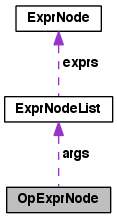
\includegraphics[width=160pt]{struct_op_expr_node__coll__graph}
\end{center}
\end{figure}
\subsection*{Public Attributes}
\begin{DoxyCompactItemize}
\item 
Op\-Type \hyperlink{struct_op_expr_node_a69ff4baea505db8ed32f4c4027f24ac6}{type}
\item 
\hyperlink{struct_expr_node_list}{Expr\-Node\-List} $\ast$ \hyperlink{struct_op_expr_node_a82d6f2c460a585ee3b0a46ce00ba186f}{args}
\end{DoxyCompactItemize}


\subsection{Detailed Description}
Stores an operation expression. An operation expression evaluates to the result of the operation performed on its arguments.

\begin{DoxySeeAlso}{See also}
create\-Op\-Expr\-Node(\-Op\-Type, Expr\-Node\-List $\ast$) 

delete\-Op\-Expr\-Node(\-Op\-Expr\-Node $\ast$) 
\end{DoxySeeAlso}


Definition at line 517 of file parser.\-h.



\subsection{Member Data Documentation}
\hypertarget{struct_op_expr_node_a82d6f2c460a585ee3b0a46ce00ba186f}{\index{Op\-Expr\-Node@{Op\-Expr\-Node}!args@{args}}
\index{args@{args}!OpExprNode@{Op\-Expr\-Node}}
\subsubsection[{args}]{\setlength{\rightskip}{0pt plus 5cm}{\bf Expr\-Node\-List}$\ast$ {\bf Op\-Expr\-Node\-::args}}}\label{struct_op_expr_node_a82d6f2c460a585ee3b0a46ce00ba186f}
A pointer to the arguments to perform the operation on. 

Definition at line 519 of file parser.\-h.

\hypertarget{struct_op_expr_node_a69ff4baea505db8ed32f4c4027f24ac6}{\index{Op\-Expr\-Node@{Op\-Expr\-Node}!type@{type}}
\index{type@{type}!OpExprNode@{Op\-Expr\-Node}}
\subsubsection[{type}]{\setlength{\rightskip}{0pt plus 5cm}Op\-Type {\bf Op\-Expr\-Node\-::type}}}\label{struct_op_expr_node_a69ff4baea505db8ed32f4c4027f24ac6}
The type of operation to perform on {\itshape args\/}. 

Definition at line 518 of file parser.\-h.



The documentation for this struct was generated from the following file\-:\begin{DoxyCompactItemize}
\item 
tools/lci/lciframework/parser.\-h\end{DoxyCompactItemize}

\hypertarget{structpcre__callout__block}{\section{pcre\-\_\-callout\-\_\-block Struct Reference}
\label{structpcre__callout__block}\index{pcre\-\_\-callout\-\_\-block@{pcre\-\_\-callout\-\_\-block}}
}
\subsection*{Public Attributes}
\begin{DoxyCompactItemize}
\item 
\hypertarget{structpcre__callout__block_ab8744d79c7a630e6edc959c0448dd6c6}{int {\bfseries version}}\label{structpcre__callout__block_ab8744d79c7a630e6edc959c0448dd6c6}

\item 
\hypertarget{structpcre__callout__block_ae6cd8e933475a4262a84f048b26a6fae}{int {\bfseries callout\-\_\-number}}\label{structpcre__callout__block_ae6cd8e933475a4262a84f048b26a6fae}

\item 
\hypertarget{structpcre__callout__block_aca28035a2b93925e6de0f60ad26dd9a5}{int $\ast$ {\bfseries offset\-\_\-vector}}\label{structpcre__callout__block_aca28035a2b93925e6de0f60ad26dd9a5}

\item 
\hypertarget{structpcre__callout__block_a32ba89aaea529364a257fa6ac769c5d4}{P\-C\-R\-E\-\_\-\-S\-P\-T\-R {\bfseries subject}}\label{structpcre__callout__block_a32ba89aaea529364a257fa6ac769c5d4}

\item 
\hypertarget{structpcre__callout__block_aa133d9f7230651e5b6d8fe05764d2f39}{int {\bfseries subject\-\_\-length}}\label{structpcre__callout__block_aa133d9f7230651e5b6d8fe05764d2f39}

\item 
\hypertarget{structpcre__callout__block_a71f4562be6b02d47eed54870f36ea791}{int {\bfseries start\-\_\-match}}\label{structpcre__callout__block_a71f4562be6b02d47eed54870f36ea791}

\item 
\hypertarget{structpcre__callout__block_a0472db6a3cc0bb069ee8e4acf36da8b5}{int {\bfseries current\-\_\-position}}\label{structpcre__callout__block_a0472db6a3cc0bb069ee8e4acf36da8b5}

\item 
\hypertarget{structpcre__callout__block_a7c73d01fc698e0a05699fa4ef4e5b48a}{int {\bfseries capture\-\_\-top}}\label{structpcre__callout__block_a7c73d01fc698e0a05699fa4ef4e5b48a}

\item 
\hypertarget{structpcre__callout__block_a989a280260effb9bf1521046a2507643}{int {\bfseries capture\-\_\-last}}\label{structpcre__callout__block_a989a280260effb9bf1521046a2507643}

\item 
\hypertarget{structpcre__callout__block_ae3b27d5cbb39957e227b09fc8d7d189c}{void $\ast$ {\bfseries callout\-\_\-data}}\label{structpcre__callout__block_ae3b27d5cbb39957e227b09fc8d7d189c}

\item 
\hypertarget{structpcre__callout__block_ac5caf602fa5ab812f8721451320b7adf}{int {\bfseries pattern\-\_\-position}}\label{structpcre__callout__block_ac5caf602fa5ab812f8721451320b7adf}

\item 
\hypertarget{structpcre__callout__block_a9360879d608b622daef0c7d1cf2606be}{int {\bfseries next\-\_\-item\-\_\-length}}\label{structpcre__callout__block_a9360879d608b622daef0c7d1cf2606be}

\end{DoxyCompactItemize}


\subsection{Detailed Description}


Definition at line 227 of file pcre.\-h.



The documentation for this struct was generated from the following files\-:\begin{DoxyCompactItemize}
\item 
Legiscode.\-applescript/build/\-Debug/\-Legiscode.\-applescript.\-app/\-Contents/\-Frameworks/\-Regex\-Kit.\-framework/\-Versions/\-A/\-Headers/pcre.\-h\item 
Legiscode.\-applescript/\-Regex\-Kit.\-framework/\-Versions/\-A/\-Headers/pcre.\-h\end{DoxyCompactItemize}

\input{structpcre__extra}
\input{struct_print_stmt_node}
\input{struct_return_object}
\hypertarget{struct_return_stmt_node}{\section{Return\-Stmt\-Node Struct Reference}
\label{struct_return_stmt_node}\index{Return\-Stmt\-Node@{Return\-Stmt\-Node}}
}


{\ttfamily \#include $<$parser.\-h$>$}



Collaboration diagram for Return\-Stmt\-Node\-:
\nopagebreak
\begin{figure}[H]
\begin{center}
\leavevmode
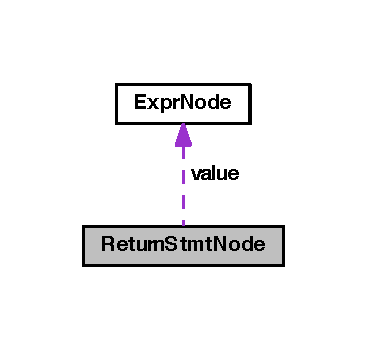
\includegraphics[width=176pt]{struct_return_stmt_node__coll__graph}
\end{center}
\end{figure}
\subsection*{Public Attributes}
\begin{DoxyCompactItemize}
\item 
\hyperlink{struct_expr_node}{Expr\-Node} $\ast$ \hyperlink{struct_return_stmt_node_ac610b54406ae3bc54e3d5c4e9fcb1d2e}{value}
\end{DoxyCompactItemize}


\subsection{Detailed Description}
Stores a return statement. A return statement signals that the current function is to be returned from with value {\itshape value\/}.

\begin{DoxySeeAlso}{See also}
create\-Return\-Stmt\-Node(\-Expr\-Node $\ast$) 

delete\-Return\-Stmt\-Node(\-Return\-Stmt\-Node $\ast$) 
\end{DoxySeeAlso}


Definition at line 447 of file parser.\-h.



\subsection{Member Data Documentation}
\hypertarget{struct_return_stmt_node_ac610b54406ae3bc54e3d5c4e9fcb1d2e}{\index{Return\-Stmt\-Node@{Return\-Stmt\-Node}!value@{value}}
\index{value@{value}!ReturnStmtNode@{Return\-Stmt\-Node}}
\subsubsection[{value}]{\setlength{\rightskip}{0pt plus 5cm}{\bf Expr\-Node}$\ast$ {\bf Return\-Stmt\-Node\-::value}}}\label{struct_return_stmt_node_ac610b54406ae3bc54e3d5c4e9fcb1d2e}
A pointer to the value to return. 

Definition at line 448 of file parser.\-h.



The documentation for this struct was generated from the following file\-:\begin{DoxyCompactItemize}
\item 
tools/lci/lciframework/parser.\-h\end{DoxyCompactItemize}

\hypertarget{interface_r_k_cache}{\section{R\-K\-Cache Class Reference}
\label{interface_r_k_cache}\index{R\-K\-Cache@{R\-K\-Cache}}
}
\subsection*{Public Member Functions}
\begin{DoxyCompactItemize}
\item 
\hypertarget{interface_r_k_cache_aaf18e92c4fd0db1f5117f9deaf096a2a}{(id) -\/ {\bfseries init\-With\-Description\-:}}\label{interface_r_k_cache_aaf18e92c4fd0db1f5117f9deaf096a2a}

\item 
\hypertarget{interface_r_k_cache_a8327b3db1c417a50a96bb0c50afe5310}{(void) -\/ {\bfseries set\-Description\-:}}\label{interface_r_k_cache_a8327b3db1c417a50a96bb0c50afe5310}

\item 
\hypertarget{interface_r_k_cache_a75bd37caf28b7fe26a01765ee50f8c39}{(N\-S\-String $\ast$) -\/ {\bfseries status}}\label{interface_r_k_cache_a75bd37caf28b7fe26a01765ee50f8c39}

\item 
\hypertarget{interface_r_k_cache_aa505f34d77ea1400b44c67fc17118ce1}{(N\-S\-String $\ast$) -\/ {\bfseries description}}\label{interface_r_k_cache_aa505f34d77ea1400b44c67fc17118ce1}

\item 
\hypertarget{interface_r_k_cache_a62d1c6218dd542a4a3f01bbf4c30d4f7}{(id) -\/ {\bfseries object\-For\-Hash\-:description\-:}}\label{interface_r_k_cache_a62d1c6218dd542a4a3f01bbf4c30d4f7}

\item 
\hypertarget{interface_r_k_cache_a78c4419a25cce30b95985cd0a1ada575}{(id) -\/ {\bfseries object\-For\-Hash\-:description\-:autorelease\-:}}\label{interface_r_k_cache_a78c4419a25cce30b95985cd0a1ada575}

\item 
\hypertarget{interface_r_k_cache_a48d6429147670a2fa30f13ac84448a81}{(B\-O\-O\-L) -\/ {\bfseries add\-Object\-To\-Cache\-:}}\label{interface_r_k_cache_a48d6429147670a2fa30f13ac84448a81}

\item 
\hypertarget{interface_r_k_cache_a7ef84b23e8b4a1dbf23ec32fef5215d4}{(B\-O\-O\-L) -\/ {\bfseries add\-Object\-To\-Cache\-:with\-Hash\-:}}\label{interface_r_k_cache_a7ef84b23e8b4a1dbf23ec32fef5215d4}

\item 
\hypertarget{interface_r_k_cache_ab0c29316fd50266177d5d158d3011a9e}{(id) -\/ {\bfseries remove\-Object\-From\-Cache\-:}}\label{interface_r_k_cache_ab0c29316fd50266177d5d158d3011a9e}

\item 
\hypertarget{interface_r_k_cache_a86e4753d32e6f6b0ce836b4eb848c26e}{(id) -\/ {\bfseries remove\-Object\-With\-Hash\-:}}\label{interface_r_k_cache_a86e4753d32e6f6b0ce836b4eb848c26e}

\item 
\hypertarget{interface_r_k_cache_a3f4c2980380e14ff2fd349c1c57aa4ae}{(B\-O\-O\-L) -\/ {\bfseries clear\-Cache}}\label{interface_r_k_cache_a3f4c2980380e14ff2fd349c1c57aa4ae}

\item 
\hypertarget{interface_r_k_cache_a2cf91ff4dec992413969d5bbd888a8e5}{(N\-S\-Set $\ast$) -\/ {\bfseries cache\-Set}}\label{interface_r_k_cache_a2cf91ff4dec992413969d5bbd888a8e5}

\item 
\hypertarget{interface_r_k_cache_a350e9b37c0bac4ed34b4f3162224dcd1}{(B\-O\-O\-L) -\/ {\bfseries is\-Cache\-Enabled}}\label{interface_r_k_cache_a350e9b37c0bac4ed34b4f3162224dcd1}

\item 
\hypertarget{interface_r_k_cache_aa4c65edbe337fe52bb6d55f4980eb871}{(B\-O\-O\-L) -\/ {\bfseries set\-Cache\-Enabled\-:}}\label{interface_r_k_cache_aa4c65edbe337fe52bb6d55f4980eb871}

\item 
\hypertarget{interface_r_k_cache_a2a6434cfb1b87ec11eaae2378644b8ad}{(R\-K\-U\-Integer) -\/ {\bfseries cache\-Count}}\label{interface_r_k_cache_a2a6434cfb1b87ec11eaae2378644b8ad}

\item 
\hypertarget{interface_r_k_cache_aaf18e92c4fd0db1f5117f9deaf096a2a}{(id) -\/ {\bfseries init\-With\-Description\-:}}\label{interface_r_k_cache_aaf18e92c4fd0db1f5117f9deaf096a2a}

\item 
\hypertarget{interface_r_k_cache_a8327b3db1c417a50a96bb0c50afe5310}{(void) -\/ {\bfseries set\-Description\-:}}\label{interface_r_k_cache_a8327b3db1c417a50a96bb0c50afe5310}

\item 
\hypertarget{interface_r_k_cache_a75bd37caf28b7fe26a01765ee50f8c39}{(N\-S\-String $\ast$) -\/ {\bfseries status}}\label{interface_r_k_cache_a75bd37caf28b7fe26a01765ee50f8c39}

\item 
\hypertarget{interface_r_k_cache_aa505f34d77ea1400b44c67fc17118ce1}{(N\-S\-String $\ast$) -\/ {\bfseries description}}\label{interface_r_k_cache_aa505f34d77ea1400b44c67fc17118ce1}

\item 
\hypertarget{interface_r_k_cache_a62d1c6218dd542a4a3f01bbf4c30d4f7}{(id) -\/ {\bfseries object\-For\-Hash\-:description\-:}}\label{interface_r_k_cache_a62d1c6218dd542a4a3f01bbf4c30d4f7}

\item 
\hypertarget{interface_r_k_cache_a78c4419a25cce30b95985cd0a1ada575}{(id) -\/ {\bfseries object\-For\-Hash\-:description\-:autorelease\-:}}\label{interface_r_k_cache_a78c4419a25cce30b95985cd0a1ada575}

\item 
\hypertarget{interface_r_k_cache_a48d6429147670a2fa30f13ac84448a81}{(B\-O\-O\-L) -\/ {\bfseries add\-Object\-To\-Cache\-:}}\label{interface_r_k_cache_a48d6429147670a2fa30f13ac84448a81}

\item 
\hypertarget{interface_r_k_cache_a7ef84b23e8b4a1dbf23ec32fef5215d4}{(B\-O\-O\-L) -\/ {\bfseries add\-Object\-To\-Cache\-:with\-Hash\-:}}\label{interface_r_k_cache_a7ef84b23e8b4a1dbf23ec32fef5215d4}

\item 
\hypertarget{interface_r_k_cache_ab0c29316fd50266177d5d158d3011a9e}{(id) -\/ {\bfseries remove\-Object\-From\-Cache\-:}}\label{interface_r_k_cache_ab0c29316fd50266177d5d158d3011a9e}

\item 
\hypertarget{interface_r_k_cache_a86e4753d32e6f6b0ce836b4eb848c26e}{(id) -\/ {\bfseries remove\-Object\-With\-Hash\-:}}\label{interface_r_k_cache_a86e4753d32e6f6b0ce836b4eb848c26e}

\item 
\hypertarget{interface_r_k_cache_a3f4c2980380e14ff2fd349c1c57aa4ae}{(B\-O\-O\-L) -\/ {\bfseries clear\-Cache}}\label{interface_r_k_cache_a3f4c2980380e14ff2fd349c1c57aa4ae}

\item 
\hypertarget{interface_r_k_cache_a2cf91ff4dec992413969d5bbd888a8e5}{(N\-S\-Set $\ast$) -\/ {\bfseries cache\-Set}}\label{interface_r_k_cache_a2cf91ff4dec992413969d5bbd888a8e5}

\item 
\hypertarget{interface_r_k_cache_a350e9b37c0bac4ed34b4f3162224dcd1}{(B\-O\-O\-L) -\/ {\bfseries is\-Cache\-Enabled}}\label{interface_r_k_cache_a350e9b37c0bac4ed34b4f3162224dcd1}

\item 
\hypertarget{interface_r_k_cache_aa4c65edbe337fe52bb6d55f4980eb871}{(B\-O\-O\-L) -\/ {\bfseries set\-Cache\-Enabled\-:}}\label{interface_r_k_cache_aa4c65edbe337fe52bb6d55f4980eb871}

\item 
\hypertarget{interface_r_k_cache_a2a6434cfb1b87ec11eaae2378644b8ad}{(R\-K\-U\-Integer) -\/ {\bfseries cache\-Count}}\label{interface_r_k_cache_a2a6434cfb1b87ec11eaae2378644b8ad}

\item 
\hypertarget{interface_r_k_cache_a8146789e53cc4f737647bc4ddabd7040}{(B\-O\-O\-L) -\/ {\bfseries is\-Cache\-Adding\-Enabled}}\label{interface_r_k_cache_a8146789e53cc4f737647bc4ddabd7040}

\item 
\hypertarget{interface_r_k_cache_a8146789e53cc4f737647bc4ddabd7040}{(B\-O\-O\-L) -\/ {\bfseries is\-Cache\-Adding\-Enabled}}\label{interface_r_k_cache_a8146789e53cc4f737647bc4ddabd7040}

\item 
\hypertarget{interface_r_k_cache_a8485a0948458929c1696239458f9d0e5}{(B\-O\-O\-L) -\/ {\bfseries set\-Cache\-Adding\-Enabled\-:}}\label{interface_r_k_cache_a8485a0948458929c1696239458f9d0e5}

\item 
\hypertarget{interface_r_k_cache_a8485a0948458929c1696239458f9d0e5}{(B\-O\-O\-L) -\/ {\bfseries set\-Cache\-Adding\-Enabled\-:}}\label{interface_r_k_cache_a8485a0948458929c1696239458f9d0e5}

\item 
\hypertarget{interface_r_k_cache_a0ebca3cdacd1adb6cd1c850c029014a0}{(B\-O\-O\-L) -\/ {\bfseries is\-Cache\-Lookup\-Enabled}}\label{interface_r_k_cache_a0ebca3cdacd1adb6cd1c850c029014a0}

\item 
\hypertarget{interface_r_k_cache_a0ebca3cdacd1adb6cd1c850c029014a0}{(B\-O\-O\-L) -\/ {\bfseries is\-Cache\-Lookup\-Enabled}}\label{interface_r_k_cache_a0ebca3cdacd1adb6cd1c850c029014a0}

\item 
\hypertarget{interface_r_k_cache_a8d0f480ed2e6ff71d8f759df45320e40}{(B\-O\-O\-L) -\/ {\bfseries set\-Cache\-Lookup\-Enabled\-:}}\label{interface_r_k_cache_a8d0f480ed2e6ff71d8f759df45320e40}

\item 
\hypertarget{interface_r_k_cache_a8d0f480ed2e6ff71d8f759df45320e40}{(B\-O\-O\-L) -\/ {\bfseries set\-Cache\-Lookup\-Enabled\-:}}\label{interface_r_k_cache_a8d0f480ed2e6ff71d8f759df45320e40}

\item 
\hypertarget{interface_r_k_cache_abc38aebb52de17d831441622d2032bfd}{(void) -\/ {\bfseries set\-Debug\-:}}\label{interface_r_k_cache_abc38aebb52de17d831441622d2032bfd}

\item 
\hypertarget{interface_r_k_cache_abc38aebb52de17d831441622d2032bfd}{(void) -\/ {\bfseries set\-Debug\-:}}\label{interface_r_k_cache_abc38aebb52de17d831441622d2032bfd}

\item 
\hypertarget{interface_r_k_cache_a8fa52ed7c9aa6ee33bfaeef174cf996b}{(void) -\/ {\bfseries clear\-Counters}}\label{interface_r_k_cache_a8fa52ed7c9aa6ee33bfaeef174cf996b}

\item 
\hypertarget{interface_r_k_cache_a8fa52ed7c9aa6ee33bfaeef174cf996b}{(void) -\/ {\bfseries clear\-Counters}}\label{interface_r_k_cache_a8fa52ed7c9aa6ee33bfaeef174cf996b}

\item 
\hypertarget{interface_r_k_cache_aef00dc526ad9b5db4e3b41c97c1f3a44}{(R\-K\-U\-Integer) -\/ {\bfseries read\-Busy\-Count}}\label{interface_r_k_cache_aef00dc526ad9b5db4e3b41c97c1f3a44}

\item 
\hypertarget{interface_r_k_cache_aef00dc526ad9b5db4e3b41c97c1f3a44}{(R\-K\-U\-Integer) -\/ {\bfseries read\-Busy\-Count}}\label{interface_r_k_cache_aef00dc526ad9b5db4e3b41c97c1f3a44}

\item 
\hypertarget{interface_r_k_cache_a575e1d1135face3ffa5777375c355015}{(R\-K\-U\-Integer) -\/ {\bfseries read\-Spin\-Count}}\label{interface_r_k_cache_a575e1d1135face3ffa5777375c355015}

\item 
\hypertarget{interface_r_k_cache_a575e1d1135face3ffa5777375c355015}{(R\-K\-U\-Integer) -\/ {\bfseries read\-Spin\-Count}}\label{interface_r_k_cache_a575e1d1135face3ffa5777375c355015}

\item 
\hypertarget{interface_r_k_cache_a8c9cd59091af9d6d85a692c1ef368709}{(R\-K\-U\-Integer) -\/ {\bfseries write\-Busy\-Count}}\label{interface_r_k_cache_a8c9cd59091af9d6d85a692c1ef368709}

\item 
\hypertarget{interface_r_k_cache_a8c9cd59091af9d6d85a692c1ef368709}{(R\-K\-U\-Integer) -\/ {\bfseries write\-Busy\-Count}}\label{interface_r_k_cache_a8c9cd59091af9d6d85a692c1ef368709}

\item 
\hypertarget{interface_r_k_cache_af488950839229f0c550f5dc5b2768d7b}{(R\-K\-U\-Integer) -\/ {\bfseries write\-Spin\-Count}}\label{interface_r_k_cache_af488950839229f0c550f5dc5b2768d7b}

\item 
\hypertarget{interface_r_k_cache_af488950839229f0c550f5dc5b2768d7b}{(R\-K\-U\-Integer) -\/ {\bfseries write\-Spin\-Count}}\label{interface_r_k_cache_af488950839229f0c550f5dc5b2768d7b}

\end{DoxyCompactItemize}
\subsection*{Protected Attributes}
\begin{DoxyCompactItemize}
\item 
\hypertarget{interface_r_k_cache_ab4e09fa7e05abeb94c0aa3957d8a483f}{R\-K\-\_\-\-S\-T\-R\-O\-N\-G\-\_\-\-R\-E\-F R\-K\-Read\-Write\-Lock $\ast$ {\bfseries cache\-R\-W\-Lock}}\label{interface_r_k_cache_ab4e09fa7e05abeb94c0aa3957d8a483f}

\item 
\hypertarget{interface_r_k_cache_a32797a8c639c51289a8b9f1fe0339b52}{R\-K\-\_\-\-S\-T\-R\-O\-N\-G\-\_\-\-R\-E\-F N\-S\-Map\-Table $\ast$ {\bfseries cache\-Map\-Table}}\label{interface_r_k_cache_a32797a8c639c51289a8b9f1fe0339b52}

\item 
\hypertarget{interface_r_k_cache_aa6784aa3007a045f34a80dc626c1ae49}{R\-K\-\_\-\-S\-T\-R\-O\-N\-G\-\_\-\-R\-E\-F N\-S\-String $\ast$ {\bfseries cache\-Description\-String}}\label{interface_r_k_cache_aa6784aa3007a045f34a80dc626c1ae49}

\item 
\hypertarget{interface_r_k_cache_a58c7fc49e9a2c023de18ac3280a123bc}{R\-K\-U\-Integer {\bfseries cache\-Hits}}\label{interface_r_k_cache_a58c7fc49e9a2c023de18ac3280a123bc}

\item 
\hypertarget{interface_r_k_cache_ab5764e41e5901d38102a13c86ec45c32}{R\-K\-U\-Integer {\bfseries cache\-Misses}}\label{interface_r_k_cache_ab5764e41e5901d38102a13c86ec45c32}

\item 
\hypertarget{interface_r_k_cache_ac0fa84e1a8956476293f50ff844c122f}{int {\bfseries cache\-Initialized}}\label{interface_r_k_cache_ac0fa84e1a8956476293f50ff844c122f}

\item 
\hypertarget{interface_r_k_cache_a5d590c45304fcf52a73443a5fbfc71e5}{int {\bfseries cache\-Is\-Enabled}}\label{interface_r_k_cache_a5d590c45304fcf52a73443a5fbfc71e5}

\item 
\hypertarget{interface_r_k_cache_ad7ed0e393fef5cda5eca414255d1d3bb}{int {\bfseries cache\-Adding\-Is\-Enabled}}\label{interface_r_k_cache_ad7ed0e393fef5cda5eca414255d1d3bb}

\item 
\hypertarget{interface_r_k_cache_a72877458d42aa5b824fe309afd70db74}{int {\bfseries cache\-Lookup\-Is\-Enabled}}\label{interface_r_k_cache_a72877458d42aa5b824fe309afd70db74}

\item 
\hypertarget{interface_r_k_cache_ad013c4163ffb5bb1b28953d60b4d5baf}{R\-K\-\_\-\-S\-T\-R\-O\-N\-G\-\_\-\-R\-E\-F char $\ast$ {\bfseries cache\-Description\-U\-T\-F8\-String}}\label{interface_r_k_cache_ad013c4163ffb5bb1b28953d60b4d5baf}

\item 
\hypertarget{interface_r_k_cache_ab12b57ce8aba23e168b55189cf3f3048}{R\-K\-U\-Integer {\bfseries cache\-Cleared\-Count}}\label{interface_r_k_cache_ab12b57ce8aba23e168b55189cf3f3048}

\end{DoxyCompactItemize}


\subsection{Detailed Description}


Definition at line 53 of file R\-K\-Cache.\-h.



The documentation for this class was generated from the following files\-:\begin{DoxyCompactItemize}
\item 
Legiscode.\-applescript/build/\-Debug/\-Legiscode.\-applescript.\-app/\-Contents/\-Frameworks/\-Regex\-Kit.\-framework/\-Versions/\-A/\-Headers/R\-K\-Cache.\-h\item 
Legiscode.\-applescript/\-Regex\-Kit.\-framework/\-Versions/\-A/\-Headers/R\-K\-Cache.\-h\end{DoxyCompactItemize}

\hypertarget{interface_r_k_enumerator}{\section{R\-K\-Enumerator Class Reference}
\label{interface_r_k_enumerator}\index{R\-K\-Enumerator@{R\-K\-Enumerator}}
}


Collaboration diagram for R\-K\-Enumerator\-:
\nopagebreak
\begin{figure}[H]
\begin{center}
\leavevmode
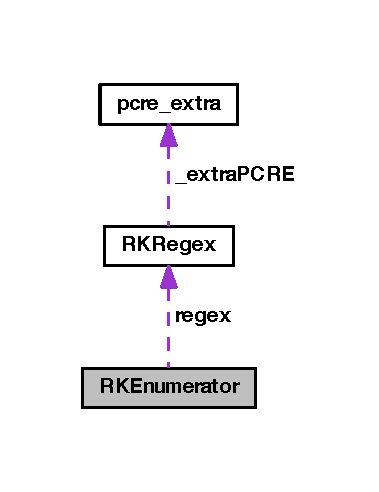
\includegraphics[width=182pt]{interface_r_k_enumerator__coll__graph}
\end{center}
\end{figure}
\subsection*{Public Member Functions}
\begin{DoxyCompactItemize}
\item 
\hypertarget{interface_r_k_enumerator_ab45fb744d0bc3a2aee41f469f4b0a986}{(id) -\/ {\bfseries init\-With\-Regex\-:string\-:}}\label{interface_r_k_enumerator_ab45fb744d0bc3a2aee41f469f4b0a986}

\item 
\hypertarget{interface_r_k_enumerator_ad1bad36f2d3bd3eba6de33fcafaf8e7b}{(id) -\/ {\bfseries init\-With\-Regex\-:string\-:in\-Range\-:}}\label{interface_r_k_enumerator_ad1bad36f2d3bd3eba6de33fcafaf8e7b}

\item 
\hypertarget{interface_r_k_enumerator_a4f1db961c794b75d4317c4a8e8208051}{(id) -\/ {\bfseries init\-With\-Regex\-:string\-:in\-Range\-:error\-:}}\label{interface_r_k_enumerator_a4f1db961c794b75d4317c4a8e8208051}

\item 
\hypertarget{interface_r_k_enumerator_ac308ce07de2295cc25e79ba95e8d1dee}{(\hyperlink{interface_r_k_regex}{R\-K\-Regex} $\ast$) -\/ {\bfseries regex}}\label{interface_r_k_enumerator_ac308ce07de2295cc25e79ba95e8d1dee}

\item 
\hypertarget{interface_r_k_enumerator_a65957082b543324f052a437183733b03}{(N\-S\-String $\ast$) -\/ {\bfseries string}}\label{interface_r_k_enumerator_a65957082b543324f052a437183733b03}

\item 
\hypertarget{interface_r_k_enumerator_ae5528582796723abbb37baca026f43e8}{(N\-S\-Range) -\/ {\bfseries current\-Range}}\label{interface_r_k_enumerator_ae5528582796723abbb37baca026f43e8}

\item 
\hypertarget{interface_r_k_enumerator_afcf75c6d91df537643c95fa25a66de92}{(N\-S\-Range) -\/ {\bfseries current\-Range\-For\-Capture\-:}}\label{interface_r_k_enumerator_afcf75c6d91df537643c95fa25a66de92}

\item 
\hypertarget{interface_r_k_enumerator_a0495dff66d2fb56a77565dfc394d3ec0}{(N\-S\-Range) -\/ {\bfseries current\-Range\-For\-Capture\-Name\-:}}\label{interface_r_k_enumerator_a0495dff66d2fb56a77565dfc394d3ec0}

\item 
\hypertarget{interface_r_k_enumerator_a7dbff5d0073d593ce26461924da6d781}{(N\-S\-Range $\ast$) -\/ {\bfseries current\-Ranges}}\label{interface_r_k_enumerator_a7dbff5d0073d593ce26461924da6d781}

\item 
\hypertarget{interface_r_k_enumerator_a61ed4826271f0a4b28442c3068938cb4}{(id) -\/ {\bfseries next\-Object}}\label{interface_r_k_enumerator_a61ed4826271f0a4b28442c3068938cb4}

\item 
\hypertarget{interface_r_k_enumerator_a91fbeeac55fb651ff57d2dde85dda012}{(N\-S\-Range) -\/ {\bfseries next\-Range}}\label{interface_r_k_enumerator_a91fbeeac55fb651ff57d2dde85dda012}

\item 
\hypertarget{interface_r_k_enumerator_a52cf789fbf7fb3cbf4ed1032fa136017}{(N\-S\-Range) -\/ {\bfseries next\-Range\-For\-Capture\-:}}\label{interface_r_k_enumerator_a52cf789fbf7fb3cbf4ed1032fa136017}

\item 
\hypertarget{interface_r_k_enumerator_a4095a601af15dd62836adeb7105f88da}{(N\-S\-Range) -\/ {\bfseries next\-Range\-For\-Capture\-Name\-:}}\label{interface_r_k_enumerator_a4095a601af15dd62836adeb7105f88da}

\item 
\hypertarget{interface_r_k_enumerator_abbc9000769aeff849cf72e7ab527f760}{(N\-S\-Range $\ast$) -\/ {\bfseries next\-Ranges}}\label{interface_r_k_enumerator_abbc9000769aeff849cf72e7ab527f760}

\item 
\hypertarget{interface_r_k_enumerator_a1c0b4f336d4d2d43502f1589eab6023e}{(B\-O\-O\-L) -\/ {\bfseries get\-Captures\-With\-References\-:}}\label{interface_r_k_enumerator_a1c0b4f336d4d2d43502f1589eab6023e}

\item 
\hypertarget{interface_r_k_enumerator_a5fb7502952ee16f65bf61fa9c4ac72f3}{(N\-S\-String $\ast$) -\/ {\bfseries string\-With\-Reference\-String\-:}}\label{interface_r_k_enumerator_a5fb7502952ee16f65bf61fa9c4ac72f3}

\item 
\hypertarget{interface_r_k_enumerator_a541989a32e34fd28d84006904a96bd31}{(N\-S\-String $\ast$) -\/ {\bfseries string\-With\-Reference\-Format\-:}}\label{interface_r_k_enumerator_a541989a32e34fd28d84006904a96bd31}

\item 
\hypertarget{interface_r_k_enumerator_a22ac0d889cf2c09c315ac08f2c750cf7}{(N\-S\-String $\ast$) -\/ {\bfseries string\-With\-Reference\-Format\-:arguments\-:}}\label{interface_r_k_enumerator_a22ac0d889cf2c09c315ac08f2c750cf7}

\item 
\hypertarget{interface_r_k_enumerator_ab45fb744d0bc3a2aee41f469f4b0a986}{(id) -\/ {\bfseries init\-With\-Regex\-:string\-:}}\label{interface_r_k_enumerator_ab45fb744d0bc3a2aee41f469f4b0a986}

\item 
\hypertarget{interface_r_k_enumerator_ad1bad36f2d3bd3eba6de33fcafaf8e7b}{(id) -\/ {\bfseries init\-With\-Regex\-:string\-:in\-Range\-:}}\label{interface_r_k_enumerator_ad1bad36f2d3bd3eba6de33fcafaf8e7b}

\item 
\hypertarget{interface_r_k_enumerator_a4f1db961c794b75d4317c4a8e8208051}{(id) -\/ {\bfseries init\-With\-Regex\-:string\-:in\-Range\-:error\-:}}\label{interface_r_k_enumerator_a4f1db961c794b75d4317c4a8e8208051}

\item 
\hypertarget{interface_r_k_enumerator_ac308ce07de2295cc25e79ba95e8d1dee}{(\hyperlink{interface_r_k_regex}{R\-K\-Regex} $\ast$) -\/ {\bfseries regex}}\label{interface_r_k_enumerator_ac308ce07de2295cc25e79ba95e8d1dee}

\item 
\hypertarget{interface_r_k_enumerator_a65957082b543324f052a437183733b03}{(N\-S\-String $\ast$) -\/ {\bfseries string}}\label{interface_r_k_enumerator_a65957082b543324f052a437183733b03}

\item 
\hypertarget{interface_r_k_enumerator_ae5528582796723abbb37baca026f43e8}{(N\-S\-Range) -\/ {\bfseries current\-Range}}\label{interface_r_k_enumerator_ae5528582796723abbb37baca026f43e8}

\item 
\hypertarget{interface_r_k_enumerator_afcf75c6d91df537643c95fa25a66de92}{(N\-S\-Range) -\/ {\bfseries current\-Range\-For\-Capture\-:}}\label{interface_r_k_enumerator_afcf75c6d91df537643c95fa25a66de92}

\item 
\hypertarget{interface_r_k_enumerator_a0495dff66d2fb56a77565dfc394d3ec0}{(N\-S\-Range) -\/ {\bfseries current\-Range\-For\-Capture\-Name\-:}}\label{interface_r_k_enumerator_a0495dff66d2fb56a77565dfc394d3ec0}

\item 
\hypertarget{interface_r_k_enumerator_a7dbff5d0073d593ce26461924da6d781}{(N\-S\-Range $\ast$) -\/ {\bfseries current\-Ranges}}\label{interface_r_k_enumerator_a7dbff5d0073d593ce26461924da6d781}

\item 
\hypertarget{interface_r_k_enumerator_a61ed4826271f0a4b28442c3068938cb4}{(id) -\/ {\bfseries next\-Object}}\label{interface_r_k_enumerator_a61ed4826271f0a4b28442c3068938cb4}

\item 
\hypertarget{interface_r_k_enumerator_a91fbeeac55fb651ff57d2dde85dda012}{(N\-S\-Range) -\/ {\bfseries next\-Range}}\label{interface_r_k_enumerator_a91fbeeac55fb651ff57d2dde85dda012}

\item 
\hypertarget{interface_r_k_enumerator_a52cf789fbf7fb3cbf4ed1032fa136017}{(N\-S\-Range) -\/ {\bfseries next\-Range\-For\-Capture\-:}}\label{interface_r_k_enumerator_a52cf789fbf7fb3cbf4ed1032fa136017}

\item 
\hypertarget{interface_r_k_enumerator_a4095a601af15dd62836adeb7105f88da}{(N\-S\-Range) -\/ {\bfseries next\-Range\-For\-Capture\-Name\-:}}\label{interface_r_k_enumerator_a4095a601af15dd62836adeb7105f88da}

\item 
\hypertarget{interface_r_k_enumerator_abbc9000769aeff849cf72e7ab527f760}{(N\-S\-Range $\ast$) -\/ {\bfseries next\-Ranges}}\label{interface_r_k_enumerator_abbc9000769aeff849cf72e7ab527f760}

\item 
\hypertarget{interface_r_k_enumerator_a1c0b4f336d4d2d43502f1589eab6023e}{(B\-O\-O\-L) -\/ {\bfseries get\-Captures\-With\-References\-:}}\label{interface_r_k_enumerator_a1c0b4f336d4d2d43502f1589eab6023e}

\item 
\hypertarget{interface_r_k_enumerator_a5fb7502952ee16f65bf61fa9c4ac72f3}{(N\-S\-String $\ast$) -\/ {\bfseries string\-With\-Reference\-String\-:}}\label{interface_r_k_enumerator_a5fb7502952ee16f65bf61fa9c4ac72f3}

\item 
\hypertarget{interface_r_k_enumerator_a541989a32e34fd28d84006904a96bd31}{(N\-S\-String $\ast$) -\/ {\bfseries string\-With\-Reference\-Format\-:}}\label{interface_r_k_enumerator_a541989a32e34fd28d84006904a96bd31}

\item 
\hypertarget{interface_r_k_enumerator_a22ac0d889cf2c09c315ac08f2c750cf7}{(N\-S\-String $\ast$) -\/ {\bfseries string\-With\-Reference\-Format\-:arguments\-:}}\label{interface_r_k_enumerator_a22ac0d889cf2c09c315ac08f2c750cf7}

\end{DoxyCompactItemize}
\subsection*{Static Public Member Functions}
\begin{DoxyCompactItemize}
\item 
\hypertarget{interface_r_k_enumerator_a68e613dc4d7b465896311f90242d9ec0}{(id) + {\bfseries enumerator\-With\-Regex\-:string\-:}}\label{interface_r_k_enumerator_a68e613dc4d7b465896311f90242d9ec0}

\item 
\hypertarget{interface_r_k_enumerator_a42ca094bc7747676b568ff967140e8cb}{(id) + {\bfseries enumerator\-With\-Regex\-:string\-:in\-Range\-:}}\label{interface_r_k_enumerator_a42ca094bc7747676b568ff967140e8cb}

\item 
\hypertarget{interface_r_k_enumerator_a19eb1be48091d8d15d97dff122c64a17}{(id) + {\bfseries enumerator\-With\-Regex\-:string\-:in\-Range\-:error\-:}}\label{interface_r_k_enumerator_a19eb1be48091d8d15d97dff122c64a17}

\item 
\hypertarget{interface_r_k_enumerator_a68e613dc4d7b465896311f90242d9ec0}{(id) + {\bfseries enumerator\-With\-Regex\-:string\-:}}\label{interface_r_k_enumerator_a68e613dc4d7b465896311f90242d9ec0}

\item 
\hypertarget{interface_r_k_enumerator_a42ca094bc7747676b568ff967140e8cb}{(id) + {\bfseries enumerator\-With\-Regex\-:string\-:in\-Range\-:}}\label{interface_r_k_enumerator_a42ca094bc7747676b568ff967140e8cb}

\item 
\hypertarget{interface_r_k_enumerator_a19eb1be48091d8d15d97dff122c64a17}{(id) + {\bfseries enumerator\-With\-Regex\-:string\-:in\-Range\-:error\-:}}\label{interface_r_k_enumerator_a19eb1be48091d8d15d97dff122c64a17}

\end{DoxyCompactItemize}
\subsection*{Protected Attributes}
\begin{DoxyCompactItemize}
\item 
\hypertarget{interface_r_k_enumerator_a0332230c5efcec00b481ba3a4c698962}{\hyperlink{interface_r_k_regex}{R\-K\-Regex} $\ast$ {\bfseries regex}}\label{interface_r_k_enumerator_a0332230c5efcec00b481ba3a4c698962}

\item 
\hypertarget{interface_r_k_enumerator_a02cc03bccf9bf32ce91677032a1bc364}{N\-S\-String $\ast$ {\bfseries string}}\label{interface_r_k_enumerator_a02cc03bccf9bf32ce91677032a1bc364}

\item 
\hypertarget{interface_r_k_enumerator_aee680d24622d627fee40ff7a67d4933a}{R\-K\-U\-Integer {\bfseries at\-Buffer\-Location}}\label{interface_r_k_enumerator_aee680d24622d627fee40ff7a67d4933a}

\item 
\hypertarget{interface_r_k_enumerator_a07ede92e2a0d5717b917f4ac23739418}{R\-K\-U\-Integer {\bfseries regex\-Capture\-Count}}\label{interface_r_k_enumerator_a07ede92e2a0d5717b917f4ac23739418}

\item 
\hypertarget{interface_r_k_enumerator_afd419d9a74cdd9aadb6f835dc9104a45}{N\-S\-Range {\bfseries search\-Byte\-Range}}\label{interface_r_k_enumerator_afd419d9a74cdd9aadb6f835dc9104a45}

\item 
\hypertarget{interface_r_k_enumerator_a72243e26252a6a5c6aee95715be79167}{N\-S\-Range {\bfseries search\-U\-T\-F16\-Range}}\label{interface_r_k_enumerator_a72243e26252a6a5c6aee95715be79167}

\item 
\hypertarget{interface_r_k_enumerator_a6877d05a7d43c4f27c45f0f6870592ab}{R\-K\-\_\-\-S\-T\-R\-O\-N\-G\-\_\-\-R\-E\-F N\-S\-Range $\ast$ {\bfseries result\-U\-T\-F8\-Ranges}}\label{interface_r_k_enumerator_a6877d05a7d43c4f27c45f0f6870592ab}

\item 
\hypertarget{interface_r_k_enumerator_ad0520356509cf2b3e500b7a1277a56ea}{R\-K\-\_\-\-S\-T\-R\-O\-N\-G\-\_\-\-R\-E\-F N\-S\-Range $\ast$ {\bfseries result\-U\-T\-F16\-Ranges}}\label{interface_r_k_enumerator_ad0520356509cf2b3e500b7a1277a56ea}

\item 
\hypertarget{interface_r_k_enumerator_a77c40111f73bb1c3c2ffca44e7d68b41}{R\-K\-U\-Integer {\bfseries has\-Performed\-Match}\-:1}\label{interface_r_k_enumerator_a77c40111f73bb1c3c2ffca44e7d68b41}

\end{DoxyCompactItemize}


\subsection{Detailed Description}


Definition at line 52 of file R\-K\-Enumerator.\-h.



The documentation for this class was generated from the following files\-:\begin{DoxyCompactItemize}
\item 
Legiscode.\-applescript/build/\-Debug/\-Legiscode.\-applescript.\-app/\-Contents/\-Frameworks/\-Regex\-Kit.\-framework/\-Versions/\-A/\-Headers/R\-K\-Enumerator.\-h\item 
Legiscode.\-applescript/\-Regex\-Kit.\-framework/\-Versions/\-A/\-Headers/R\-K\-Enumerator.\-h\end{DoxyCompactItemize}

\hypertarget{interface_r_k_regex}{\section{R\-K\-Regex Class Reference}
\label{interface_r_k_regex}\index{R\-K\-Regex@{R\-K\-Regex}}
}


Collaboration diagram for R\-K\-Regex\-:
\nopagebreak
\begin{figure}[H]
\begin{center}
\leavevmode
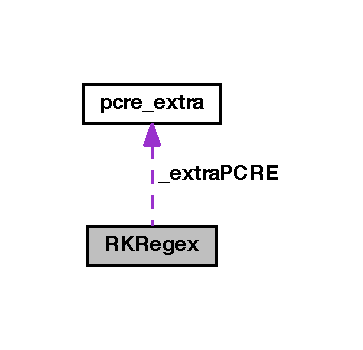
\includegraphics[width=174pt]{interface_r_k_regex__coll__graph}
\end{center}
\end{figure}
\subsection*{Public Member Functions}
\begin{DoxyCompactItemize}
\item 
\hypertarget{interface_r_k_regex_a09c782cb88bbf39417598d137cd2f179}{(id) -\/ {\bfseries init\-With\-Regex\-String\-:options\-:}}\label{interface_r_k_regex_a09c782cb88bbf39417598d137cd2f179}

\item 
\hypertarget{interface_r_k_regex_a7c3af7648115f2edb42bb59beafafc9c}{(id) -\/ {\bfseries init\-With\-Regex\-String\-:library\-:options\-:error\-:}}\label{interface_r_k_regex_a7c3af7648115f2edb42bb59beafafc9c}

\item 
\hypertarget{interface_r_k_regex_a14f61c1e7cdd39971963e66988e7f60f}{(N\-S\-String $\ast$) -\/ {\bfseries regex\-String}}\label{interface_r_k_regex_a14f61c1e7cdd39971963e66988e7f60f}

\item 
\hypertarget{interface_r_k_regex_a4a46ed536513f45f934098109159e86f}{(R\-K\-Compile\-Option) -\/ {\bfseries compile\-Option}}\label{interface_r_k_regex_a4a46ed536513f45f934098109159e86f}

\item 
\hypertarget{interface_r_k_regex_a933d645e53bc3011cf043bbe69647191}{(R\-K\-U\-Integer) -\/ {\bfseries capture\-Count}}\label{interface_r_k_regex_a933d645e53bc3011cf043bbe69647191}

\item 
\hypertarget{interface_r_k_regex_a85c7c3e1008c41063a3cef874bb09e5f}{(N\-S\-Array $\ast$) -\/ {\bfseries capture\-Name\-Array}}\label{interface_r_k_regex_a85c7c3e1008c41063a3cef874bb09e5f}

\item 
\hypertarget{interface_r_k_regex_a41148691b39fea4c7abeb85498044470}{(B\-O\-O\-L) -\/ {\bfseries is\-Valid\-Capture\-Name\-:}}\label{interface_r_k_regex_a41148691b39fea4c7abeb85498044470}

\item 
\hypertarget{interface_r_k_regex_a64f0e9b631149094cc7227adb0a2ec39}{(R\-K\-U\-Integer) -\/ {\bfseries capture\-Index\-For\-Capture\-Name\-:}}\label{interface_r_k_regex_a64f0e9b631149094cc7227adb0a2ec39}

\item 
\hypertarget{interface_r_k_regex_adea1582c8fc35ad3408445c8467b3828}{(N\-S\-String $\ast$) -\/ {\bfseries capture\-Name\-For\-Capture\-Index\-:}}\label{interface_r_k_regex_adea1582c8fc35ad3408445c8467b3828}

\item 
\hypertarget{interface_r_k_regex_ac006c9fee29acc444c2596bf99e415cc}{(R\-K\-U\-Integer) -\/ {\bfseries capture\-Index\-For\-Capture\-Name\-:in\-Matched\-Ranges\-:}}\label{interface_r_k_regex_ac006c9fee29acc444c2596bf99e415cc}

\item 
\hypertarget{interface_r_k_regex_a54f94fa012e48e42c376908f58164e1c}{(R\-K\-U\-Integer) -\/ {\bfseries capture\-Index\-For\-Capture\-Name\-:in\-Matched\-Ranges\-:error\-:}}\label{interface_r_k_regex_a54f94fa012e48e42c376908f58164e1c}

\item 
\hypertarget{interface_r_k_regex_aa33efb469a55abee4c508f748d703aef}{(B\-O\-O\-L) -\/ {\bfseries matches\-Characters\-:length\-:in\-Range\-:options\-:}}\label{interface_r_k_regex_aa33efb469a55abee4c508f748d703aef}

\item 
\hypertarget{interface_r_k_regex_a9da47043b99002e9b5b3cb60e34a7d19}{(N\-S\-Range) -\/ {\bfseries range\-For\-Characters\-:length\-:in\-Range\-:capture\-Index\-:options\-:}}\label{interface_r_k_regex_a9da47043b99002e9b5b3cb60e34a7d19}

\item 
\hypertarget{interface_r_k_regex_a2b084eb136061edc6a39253709d145d3}{(N\-S\-Range $\ast$) -\/ {\bfseries ranges\-For\-Characters\-:length\-:in\-Range\-:options\-:}}\label{interface_r_k_regex_a2b084eb136061edc6a39253709d145d3}

\item 
\hypertarget{interface_r_k_regex_a81365eb7d809043ed0a1a27ec99c09c7}{(R\-K\-Match\-Error\-Code) -\/ {\bfseries get\-Ranges\-:with\-Characters\-:length\-:in\-Range\-:options\-:}}\label{interface_r_k_regex_a81365eb7d809043ed0a1a27ec99c09c7}

\item 
\hypertarget{interface_r_k_regex_a09c782cb88bbf39417598d137cd2f179}{(id) -\/ {\bfseries init\-With\-Regex\-String\-:options\-:}}\label{interface_r_k_regex_a09c782cb88bbf39417598d137cd2f179}

\item 
\hypertarget{interface_r_k_regex_a7c3af7648115f2edb42bb59beafafc9c}{(id) -\/ {\bfseries init\-With\-Regex\-String\-:library\-:options\-:error\-:}}\label{interface_r_k_regex_a7c3af7648115f2edb42bb59beafafc9c}

\item 
\hypertarget{interface_r_k_regex_a14f61c1e7cdd39971963e66988e7f60f}{(N\-S\-String $\ast$) -\/ {\bfseries regex\-String}}\label{interface_r_k_regex_a14f61c1e7cdd39971963e66988e7f60f}

\item 
\hypertarget{interface_r_k_regex_a4a46ed536513f45f934098109159e86f}{(R\-K\-Compile\-Option) -\/ {\bfseries compile\-Option}}\label{interface_r_k_regex_a4a46ed536513f45f934098109159e86f}

\item 
\hypertarget{interface_r_k_regex_a933d645e53bc3011cf043bbe69647191}{(R\-K\-U\-Integer) -\/ {\bfseries capture\-Count}}\label{interface_r_k_regex_a933d645e53bc3011cf043bbe69647191}

\item 
\hypertarget{interface_r_k_regex_a85c7c3e1008c41063a3cef874bb09e5f}{(N\-S\-Array $\ast$) -\/ {\bfseries capture\-Name\-Array}}\label{interface_r_k_regex_a85c7c3e1008c41063a3cef874bb09e5f}

\item 
\hypertarget{interface_r_k_regex_a41148691b39fea4c7abeb85498044470}{(B\-O\-O\-L) -\/ {\bfseries is\-Valid\-Capture\-Name\-:}}\label{interface_r_k_regex_a41148691b39fea4c7abeb85498044470}

\item 
\hypertarget{interface_r_k_regex_a64f0e9b631149094cc7227adb0a2ec39}{(R\-K\-U\-Integer) -\/ {\bfseries capture\-Index\-For\-Capture\-Name\-:}}\label{interface_r_k_regex_a64f0e9b631149094cc7227adb0a2ec39}

\item 
\hypertarget{interface_r_k_regex_adea1582c8fc35ad3408445c8467b3828}{(N\-S\-String $\ast$) -\/ {\bfseries capture\-Name\-For\-Capture\-Index\-:}}\label{interface_r_k_regex_adea1582c8fc35ad3408445c8467b3828}

\item 
\hypertarget{interface_r_k_regex_ac006c9fee29acc444c2596bf99e415cc}{(R\-K\-U\-Integer) -\/ {\bfseries capture\-Index\-For\-Capture\-Name\-:in\-Matched\-Ranges\-:}}\label{interface_r_k_regex_ac006c9fee29acc444c2596bf99e415cc}

\item 
\hypertarget{interface_r_k_regex_a54f94fa012e48e42c376908f58164e1c}{(R\-K\-U\-Integer) -\/ {\bfseries capture\-Index\-For\-Capture\-Name\-:in\-Matched\-Ranges\-:error\-:}}\label{interface_r_k_regex_a54f94fa012e48e42c376908f58164e1c}

\item 
\hypertarget{interface_r_k_regex_aa33efb469a55abee4c508f748d703aef}{(B\-O\-O\-L) -\/ {\bfseries matches\-Characters\-:length\-:in\-Range\-:options\-:}}\label{interface_r_k_regex_aa33efb469a55abee4c508f748d703aef}

\item 
\hypertarget{interface_r_k_regex_a9da47043b99002e9b5b3cb60e34a7d19}{(N\-S\-Range) -\/ {\bfseries range\-For\-Characters\-:length\-:in\-Range\-:capture\-Index\-:options\-:}}\label{interface_r_k_regex_a9da47043b99002e9b5b3cb60e34a7d19}

\item 
\hypertarget{interface_r_k_regex_a2b084eb136061edc6a39253709d145d3}{(N\-S\-Range $\ast$) -\/ {\bfseries ranges\-For\-Characters\-:length\-:in\-Range\-:options\-:}}\label{interface_r_k_regex_a2b084eb136061edc6a39253709d145d3}

\item 
\hypertarget{interface_r_k_regex_a81365eb7d809043ed0a1a27ec99c09c7}{(R\-K\-Match\-Error\-Code) -\/ {\bfseries get\-Ranges\-:with\-Characters\-:length\-:in\-Range\-:options\-:}}\label{interface_r_k_regex_a81365eb7d809043ed0a1a27ec99c09c7}

\end{DoxyCompactItemize}
\subsection*{Static Public Member Functions}
\begin{DoxyCompactItemize}
\item 
\hypertarget{interface_r_k_regex_a0df9191ede8f223b3965e064eef8a92d}{(\hyperlink{interface_r_k_cache}{R\-K\-Cache} $\ast$) + {\bfseries regex\-Cache}}\label{interface_r_k_regex_a0df9191ede8f223b3965e064eef8a92d}

\item 
\hypertarget{interface_r_k_regex_a5c0527782846c2e8b203b6a696253dec}{(N\-S\-String $\ast$) + {\bfseries P\-C\-R\-E\-Version\-String}}\label{interface_r_k_regex_a5c0527782846c2e8b203b6a696253dec}

\item 
\hypertarget{interface_r_k_regex_abd8b65cafa5f7307ab695a55c768d57f}{(int32\-\_\-t) + {\bfseries P\-C\-R\-E\-Major\-Version}}\label{interface_r_k_regex_abd8b65cafa5f7307ab695a55c768d57f}

\item 
\hypertarget{interface_r_k_regex_afd9f97672fb4f9ea18320ff196b2fc5f}{(int32\-\_\-t) + {\bfseries P\-C\-R\-E\-Minor\-Version}}\label{interface_r_k_regex_afd9f97672fb4f9ea18320ff196b2fc5f}

\item 
\hypertarget{interface_r_k_regex_a13027f32da44ae7ac6f1e436c3aefba3}{(R\-K\-Build\-Config) + {\bfseries P\-C\-R\-E\-Build\-Config}}\label{interface_r_k_regex_a13027f32da44ae7ac6f1e436c3aefba3}

\item 
\hypertarget{interface_r_k_regex_a7a32c67fbe4f41a4ef7607f637d53254}{(B\-O\-O\-L) + {\bfseries is\-Valid\-Regex\-String\-:options\-:}}\label{interface_r_k_regex_a7a32c67fbe4f41a4ef7607f637d53254}

\item 
\hypertarget{interface_r_k_regex_ae2518fd9c82197099249faf23f772d9a}{(id) + {\bfseries regex\-With\-Regex\-String\-:options\-:}}\label{interface_r_k_regex_ae2518fd9c82197099249faf23f772d9a}

\item 
\hypertarget{interface_r_k_regex_aaaa85c739d69fbe02031fdf93a7986b8}{(id) + {\bfseries regex\-With\-Regex\-String\-:library\-:options\-:error\-:}}\label{interface_r_k_regex_aaaa85c739d69fbe02031fdf93a7986b8}

\item 
\hypertarget{interface_r_k_regex_a0df9191ede8f223b3965e064eef8a92d}{(\hyperlink{interface_r_k_cache}{R\-K\-Cache} $\ast$) + {\bfseries regex\-Cache}}\label{interface_r_k_regex_a0df9191ede8f223b3965e064eef8a92d}

\item 
\hypertarget{interface_r_k_regex_a5c0527782846c2e8b203b6a696253dec}{(N\-S\-String $\ast$) + {\bfseries P\-C\-R\-E\-Version\-String}}\label{interface_r_k_regex_a5c0527782846c2e8b203b6a696253dec}

\item 
\hypertarget{interface_r_k_regex_abd8b65cafa5f7307ab695a55c768d57f}{(int32\-\_\-t) + {\bfseries P\-C\-R\-E\-Major\-Version}}\label{interface_r_k_regex_abd8b65cafa5f7307ab695a55c768d57f}

\item 
\hypertarget{interface_r_k_regex_afd9f97672fb4f9ea18320ff196b2fc5f}{(int32\-\_\-t) + {\bfseries P\-C\-R\-E\-Minor\-Version}}\label{interface_r_k_regex_afd9f97672fb4f9ea18320ff196b2fc5f}

\item 
\hypertarget{interface_r_k_regex_a13027f32da44ae7ac6f1e436c3aefba3}{(R\-K\-Build\-Config) + {\bfseries P\-C\-R\-E\-Build\-Config}}\label{interface_r_k_regex_a13027f32da44ae7ac6f1e436c3aefba3}

\item 
\hypertarget{interface_r_k_regex_a7a32c67fbe4f41a4ef7607f637d53254}{(B\-O\-O\-L) + {\bfseries is\-Valid\-Regex\-String\-:options\-:}}\label{interface_r_k_regex_a7a32c67fbe4f41a4ef7607f637d53254}

\item 
\hypertarget{interface_r_k_regex_ae2518fd9c82197099249faf23f772d9a}{(id) + {\bfseries regex\-With\-Regex\-String\-:options\-:}}\label{interface_r_k_regex_ae2518fd9c82197099249faf23f772d9a}

\item 
\hypertarget{interface_r_k_regex_aaaa85c739d69fbe02031fdf93a7986b8}{(id) + {\bfseries regex\-With\-Regex\-String\-:library\-:options\-:error\-:}}\label{interface_r_k_regex_aaaa85c739d69fbe02031fdf93a7986b8}

\end{DoxyCompactItemize}
\subsection*{Protected Attributes}
\begin{DoxyCompactItemize}
\item 
\hypertarget{interface_r_k_regex_aba50ee6e939ad021ecb102f54b8100b9}{R\-K\-\_\-\-S\-T\-R\-O\-N\-G\-\_\-\-R\-E\-F pcre $\ast$ {\bfseries \-\_\-compiled\-P\-C\-R\-E}}\label{interface_r_k_regex_aba50ee6e939ad021ecb102f54b8100b9}

\item 
\hypertarget{interface_r_k_regex_a8e19d0ef588583038126bebf45a48cdd}{R\-K\-\_\-\-S\-T\-R\-O\-N\-G\-\_\-\-R\-E\-F \hyperlink{structpcre__extra}{pcre\-\_\-extra} $\ast$ {\bfseries \-\_\-extra\-P\-C\-R\-E}}\label{interface_r_k_regex_a8e19d0ef588583038126bebf45a48cdd}

\item 
\hypertarget{interface_r_k_regex_ae146bb4ea5f568a5b4ffb541291da639}{N\-S\-String $\ast$ {\bfseries compiled\-Regex\-String}}\label{interface_r_k_regex_ae146bb4ea5f568a5b4ffb541291da639}

\item 
\hypertarget{interface_r_k_regex_a4b15de7c1dadf827b3eb21454686c7f3}{R\-K\-Compile\-Option {\bfseries compile\-Option}}\label{interface_r_k_regex_a4b15de7c1dadf827b3eb21454686c7f3}

\item 
\hypertarget{interface_r_k_regex_a2835832938eec8af92255759fc6278e4}{R\-K\-U\-Integer {\bfseries capture\-Count}}\label{interface_r_k_regex_a2835832938eec8af92255759fc6278e4}

\item 
\hypertarget{interface_r_k_regex_a986245e019741a2c91b2fd6470adef0b}{R\-K\-\_\-\-S\-T\-R\-O\-N\-G\-\_\-\-R\-E\-F char $\ast$ {\bfseries capture\-Name\-Table}}\label{interface_r_k_regex_a986245e019741a2c91b2fd6470adef0b}

\item 
\hypertarget{interface_r_k_regex_a4d23812f239a36f5d6a611ffab3a6938}{R\-K\-U\-Integer {\bfseries capture\-Name\-Table\-Length}}\label{interface_r_k_regex_a4d23812f239a36f5d6a611ffab3a6938}

\item 
\hypertarget{interface_r_k_regex_ac05b2b2d84f5680728b23438c86d9ab5}{R\-K\-U\-Integer {\bfseries capture\-Name\-Length}}\label{interface_r_k_regex_ac05b2b2d84f5680728b23438c86d9ab5}

\item 
\hypertarget{interface_r_k_regex_a0c2a48115226cca8bdeeb1c886d7bbf0}{N\-S\-Array $\ast$ {\bfseries capture\-Name\-Array}}\label{interface_r_k_regex_a0c2a48115226cca8bdeeb1c886d7bbf0}

\item 
\hypertarget{interface_r_k_regex_aa821e58d12e7065a25228b59d983da7f}{R\-K\-Integer {\bfseries reference\-Count\-Minus\-One}}\label{interface_r_k_regex_aa821e58d12e7065a25228b59d983da7f}

\item 
\hypertarget{interface_r_k_regex_a3869fc68f83830cfaf6f379043d36328}{R\-K\-U\-Integer {\bfseries hash}}\label{interface_r_k_regex_a3869fc68f83830cfaf6f379043d36328}

\item 
\hypertarget{interface_r_k_regex_aecbf394cc0b19998f4d805e4a29acf8f}{R\-K\-\_\-\-S\-T\-R\-O\-N\-G\-\_\-\-R\-E\-F char $\ast$ {\bfseries compiled\-Regex\-U\-T\-F8\-String}}\label{interface_r_k_regex_aecbf394cc0b19998f4d805e4a29acf8f}

\item 
\hypertarget{interface_r_k_regex_a9812824ffb4958269b8f3f40b12bdb9e}{R\-K\-\_\-\-S\-T\-R\-O\-N\-G\-\_\-\-R\-E\-F char $\ast$ {\bfseries compiled\-Option\-U\-T\-F8\-String}}\label{interface_r_k_regex_a9812824ffb4958269b8f3f40b12bdb9e}

\end{DoxyCompactItemize}


\subsection{Detailed Description}


Definition at line 51 of file R\-K\-Regex.\-h.



The documentation for this class was generated from the following files\-:\begin{DoxyCompactItemize}
\item 
Legiscode.\-applescript/build/\-Debug/\-Legiscode.\-applescript.\-app/\-Contents/\-Frameworks/\-Regex\-Kit.\-framework/\-Versions/\-A/\-Headers/R\-K\-Regex.\-h\item 
Legiscode.\-applescript/\-Regex\-Kit.\-framework/\-Versions/\-A/\-Headers/R\-K\-Regex.\-h\end{DoxyCompactItemize}

\input{structscopeobject}
\hypertarget{struct_stmt_node}{\section{Stmt\-Node Struct Reference}
\label{struct_stmt_node}\index{Stmt\-Node@{Stmt\-Node}}
}


{\ttfamily \#include $<$parser.\-h$>$}

\subsection*{Public Attributes}
\begin{DoxyCompactItemize}
\item 
Stmt\-Type \hyperlink{struct_stmt_node_a1a1a8ff13773a99c9344f5392cabfa13}{type}
\item 
void $\ast$ \hyperlink{struct_stmt_node_abe2bb8927d8a9a26b83d855fb14837e6}{stmt}
\end{DoxyCompactItemize}


\subsection{Detailed Description}
Stores a statement. A statement is a unit of code which can be executed by itself and may possibly cause side-\/effects to occur.

\begin{DoxySeeAlso}{See also}
create\-Stmt\-Node(\-Stmt\-Type, void $\ast$) 

delete\-Stmt\-Node(\-Stmt\-Node $\ast$) 
\end{DoxySeeAlso}


Definition at line 222 of file parser.\-h.



\subsection{Member Data Documentation}
\hypertarget{struct_stmt_node_abe2bb8927d8a9a26b83d855fb14837e6}{\index{Stmt\-Node@{Stmt\-Node}!stmt@{stmt}}
\index{stmt@{stmt}!StmtNode@{Stmt\-Node}}
\subsubsection[{stmt}]{\setlength{\rightskip}{0pt plus 5cm}void$\ast$ {\bf Stmt\-Node\-::stmt}}}\label{struct_stmt_node_abe2bb8927d8a9a26b83d855fb14837e6}
A pointer to the particular statement structure. 

Definition at line 224 of file parser.\-h.

\hypertarget{struct_stmt_node_a1a1a8ff13773a99c9344f5392cabfa13}{\index{Stmt\-Node@{Stmt\-Node}!type@{type}}
\index{type@{type}!StmtNode@{Stmt\-Node}}
\subsubsection[{type}]{\setlength{\rightskip}{0pt plus 5cm}Stmt\-Type {\bf Stmt\-Node\-::type}}}\label{struct_stmt_node_a1a1a8ff13773a99c9344f5392cabfa13}
The type of statement stored in {\itshape node\/}. 

Definition at line 223 of file parser.\-h.



The documentation for this struct was generated from the following file\-:\begin{DoxyCompactItemize}
\item 
tools/lci/lciframework/parser.\-h\end{DoxyCompactItemize}

\input{struct_stmt_node_list}
\hypertarget{struct_switch_stmt_node}{\section{Switch\-Stmt\-Node Struct Reference}
\label{struct_switch_stmt_node}\index{Switch\-Stmt\-Node@{Switch\-Stmt\-Node}}
}


{\ttfamily \#include $<$parser.\-h$>$}



Collaboration diagram for Switch\-Stmt\-Node\-:
\nopagebreak
\begin{figure}[H]
\begin{center}
\leavevmode
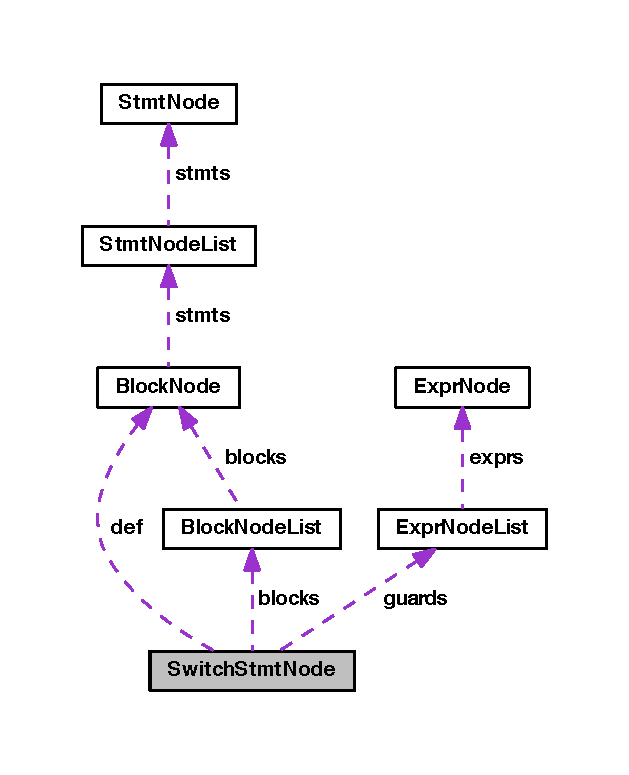
\includegraphics[width=302pt]{struct_switch_stmt_node__coll__graph}
\end{center}
\end{figure}
\subsection*{Public Attributes}
\begin{DoxyCompactItemize}
\item 
\hyperlink{struct_expr_node_list}{Expr\-Node\-List} $\ast$ \hyperlink{struct_switch_stmt_node_a125319a6fd02d72d96d41193daffb4a2}{guards}
\item 
\hyperlink{struct_block_node_list}{Block\-Node\-List} $\ast$ \hyperlink{struct_switch_stmt_node_a6cdb5c66044261b28302b6ca682d7564}{blocks}
\item 
\hyperlink{struct_block_node}{Block\-Node} $\ast$ \hyperlink{struct_switch_stmt_node_ad75de1632a46c451d251959e56d53d44}{def}
\end{DoxyCompactItemize}


\subsection{Detailed Description}
Stores a switch statement. A switch statement compares the value of the \hyperlink{impvar}{implicit variable} to each of the {\itshape guards\/} and executes the respective block of code in {\itshape blocks\/} if they match. If no matches are found between the \hyperlink{impvar}{implicit variable} and one of the {\itshape guards\/}, the optional default block of code, {\itshape def\/}, is executed.

\begin{DoxySeeAlso}{See also}
create\-Switch\-Stmt\-Node(\-Expr\-Node\-List $\ast$, Block\-Node\-List $\ast$, Block\-Node $\ast$) 

delete\-Switch\-Stmt\-Node(\-Switch\-Stmt\-Node $\ast$) 
\end{DoxySeeAlso}


Definition at line 436 of file parser.\-h.



\subsection{Member Data Documentation}
\hypertarget{struct_switch_stmt_node_a6cdb5c66044261b28302b6ca682d7564}{\index{Switch\-Stmt\-Node@{Switch\-Stmt\-Node}!blocks@{blocks}}
\index{blocks@{blocks}!SwitchStmtNode@{Switch\-Stmt\-Node}}
\subsubsection[{blocks}]{\setlength{\rightskip}{0pt plus 5cm}{\bf Block\-Node\-List}$\ast$ {\bf Switch\-Stmt\-Node\-::blocks}}}\label{struct_switch_stmt_node_a6cdb5c66044261b28302b6ca682d7564}
A pointer to the respective blocks of code to execute if one of the {\itshape guards\/} matches the \hyperlink{impvar}{implicit variable}. 

Definition at line 438 of file parser.\-h.

\hypertarget{struct_switch_stmt_node_ad75de1632a46c451d251959e56d53d44}{\index{Switch\-Stmt\-Node@{Switch\-Stmt\-Node}!def@{def}}
\index{def@{def}!SwitchStmtNode@{Switch\-Stmt\-Node}}
\subsubsection[{def}]{\setlength{\rightskip}{0pt plus 5cm}{\bf Block\-Node}$\ast$ {\bf Switch\-Stmt\-Node\-::def}}}\label{struct_switch_stmt_node_ad75de1632a46c451d251959e56d53d44}
A pointer to the default block of code to execute if none of the {\itshape guards\/} match the \hyperlink{impvar}{implicit variable}. 

Definition at line 439 of file parser.\-h.

\hypertarget{struct_switch_stmt_node_a125319a6fd02d72d96d41193daffb4a2}{\index{Switch\-Stmt\-Node@{Switch\-Stmt\-Node}!guards@{guards}}
\index{guards@{guards}!SwitchStmtNode@{Switch\-Stmt\-Node}}
\subsubsection[{guards}]{\setlength{\rightskip}{0pt plus 5cm}{\bf Expr\-Node\-List}$\ast$ {\bf Switch\-Stmt\-Node\-::guards}}}\label{struct_switch_stmt_node_a125319a6fd02d72d96d41193daffb4a2}
A pointer to the expressions to evaluate and compare to the \hyperlink{impvar}{implicit variable}. 

Definition at line 437 of file parser.\-h.



The documentation for this struct was generated from the following file\-:\begin{DoxyCompactItemize}
\item 
tools/lci/lciframework/parser.\-h\end{DoxyCompactItemize}

\input{struct_token}
\hypertarget{union_token_data}{\section{Token\-Data Union Reference}
\label{union_token_data}\index{Token\-Data@{Token\-Data}}
}


{\ttfamily \#include $<$tokenizer.\-h$>$}

\subsection*{Public Attributes}
\begin{DoxyCompactItemize}
\item 
int \hyperlink{union_token_data_aa8084a7b7f73bcce7ccfa2e17b4d3c0f}{i}
\item 
float \hyperlink{union_token_data_affb76b1c0ea30bca741d3148601fee73}{f}
\end{DoxyCompactItemize}


\subsection{Detailed Description}
Stores the data associated with a \hyperlink{struct_token}{Token} structure. 

Definition at line 161 of file tokenizer.\-h.



\subsection{Member Data Documentation}
\hypertarget{union_token_data_affb76b1c0ea30bca741d3148601fee73}{\index{Token\-Data@{Token\-Data}!f@{f}}
\index{f@{f}!TokenData@{Token\-Data}}
\subsubsection[{f}]{\setlength{\rightskip}{0pt plus 5cm}float {\bf Token\-Data\-::f}}}\label{union_token_data_affb76b1c0ea30bca741d3148601fee73}
Floating point data. 

Definition at line 163 of file tokenizer.\-h.

\hypertarget{union_token_data_aa8084a7b7f73bcce7ccfa2e17b4d3c0f}{\index{Token\-Data@{Token\-Data}!i@{i}}
\index{i@{i}!TokenData@{Token\-Data}}
\subsubsection[{i}]{\setlength{\rightskip}{0pt plus 5cm}int {\bf Token\-Data\-::i}}}\label{union_token_data_aa8084a7b7f73bcce7ccfa2e17b4d3c0f}
Integer data. 

Definition at line 162 of file tokenizer.\-h.



The documentation for this union was generated from the following file\-:\begin{DoxyCompactItemize}
\item 
tools/lci/lciframework/\hyperlink{tokenizer_8h}{tokenizer.\-h}\end{DoxyCompactItemize}

\hypertarget{struct_type_node}{\section{Type\-Node Struct Reference}
\label{struct_type_node}\index{Type\-Node@{Type\-Node}}
}


{\ttfamily \#include $<$parser.\-h$>$}

\subsection*{Public Attributes}
\begin{DoxyCompactItemize}
\item 
Constant\-Type \hyperlink{struct_type_node_abd5fc196a6f39c15eb33e94eec269ac7}{type}
\end{DoxyCompactItemize}


\subsection{Detailed Description}
Stores a variable type.

\begin{DoxySeeAlso}{See also}
create\-Type\-Node(\-Constant\-Type) 

delete\-Type\-Node(\-Type\-Node $\ast$) 
\end{DoxySeeAlso}


Definition at line 354 of file parser.\-h.



\subsection{Member Data Documentation}
\hypertarget{struct_type_node_abd5fc196a6f39c15eb33e94eec269ac7}{\index{Type\-Node@{Type\-Node}!type@{type}}
\index{type@{type}!TypeNode@{Type\-Node}}
\subsubsection[{type}]{\setlength{\rightskip}{0pt plus 5cm}Constant\-Type {\bf Type\-Node\-::type}}}\label{struct_type_node_abd5fc196a6f39c15eb33e94eec269ac7}
The type of the variable. 

Definition at line 355 of file parser.\-h.



The documentation for this struct was generated from the following file\-:\begin{DoxyCompactItemize}
\item 
tools/lci/lciframework/parser.\-h\end{DoxyCompactItemize}

\hypertarget{union_value_data}{\section{Value\-Data Union Reference}
\label{union_value_data}\index{Value\-Data@{Value\-Data}}
}


{\ttfamily \#include $<$interpreter.\-h$>$}

\subsection*{Public Attributes}
\begin{DoxyCompactItemize}
\item 
int \hyperlink{union_value_data_abc2f11fb39990140dbc322610ba52f70}{i}
\item 
float \hyperlink{union_value_data_a85311c11b54183bb571f35ed70af37a9}{f}
\item 
char $\ast$ \hyperlink{union_value_data_a2639b48549e0788d5f9a3da6ea9cb0e4}{s}
\end{DoxyCompactItemize}


\subsection{Detailed Description}
Stores the data associated with a \hyperlink{struct_value_object}{Value\-Object} structure. 

Definition at line 39 of file interpreter.\-h.



\subsection{Member Data Documentation}
\hypertarget{union_value_data_a85311c11b54183bb571f35ed70af37a9}{\index{Value\-Data@{Value\-Data}!f@{f}}
\index{f@{f}!ValueData@{Value\-Data}}
\subsubsection[{f}]{\setlength{\rightskip}{0pt plus 5cm}float {\bf Value\-Data\-::f}}}\label{union_value_data_a85311c11b54183bb571f35ed70af37a9}
Floating point data. 

Definition at line 41 of file interpreter.\-h.

\hypertarget{union_value_data_abc2f11fb39990140dbc322610ba52f70}{\index{Value\-Data@{Value\-Data}!i@{i}}
\index{i@{i}!ValueData@{Value\-Data}}
\subsubsection[{i}]{\setlength{\rightskip}{0pt plus 5cm}int {\bf Value\-Data\-::i}}}\label{union_value_data_abc2f11fb39990140dbc322610ba52f70}
Integer data. 

Definition at line 40 of file interpreter.\-h.

\hypertarget{union_value_data_a2639b48549e0788d5f9a3da6ea9cb0e4}{\index{Value\-Data@{Value\-Data}!s@{s}}
\index{s@{s}!ValueData@{Value\-Data}}
\subsubsection[{s}]{\setlength{\rightskip}{0pt plus 5cm}char$\ast$ {\bf Value\-Data\-::s}}}\label{union_value_data_a2639b48549e0788d5f9a3da6ea9cb0e4}
Character string data. 

Definition at line 42 of file interpreter.\-h.



The documentation for this union was generated from the following file\-:\begin{DoxyCompactItemize}
\item 
tools/lci/lciframework/\hyperlink{interpreter_8h}{interpreter.\-h}\end{DoxyCompactItemize}

\input{struct_value_object}
\chapter{File Documentation}
\hypertarget{interpreter_8h}{\section{tools/lci/lciframework/interpreter.h File Reference}
\label{interpreter_8h}\index{tools/lci/lciframework/interpreter.\-h@{tools/lci/lciframework/interpreter.\-h}}
}
{\ttfamily \#include $<$stdio.\-h$>$}\\*
{\ttfamily \#include $<$ctype.\-h$>$}\\*
{\ttfamily \#include $<$math.\-h$>$}\\*
{\ttfamily \#include \char`\"{}parser.\-h\char`\"{}}\\*
{\ttfamily \#include \char`\"{}unicode.\-h\char`\"{}}\\*
Include dependency graph for interpreter.\-h\-:
\nopagebreak
\begin{figure}[H]
\begin{center}
\leavevmode
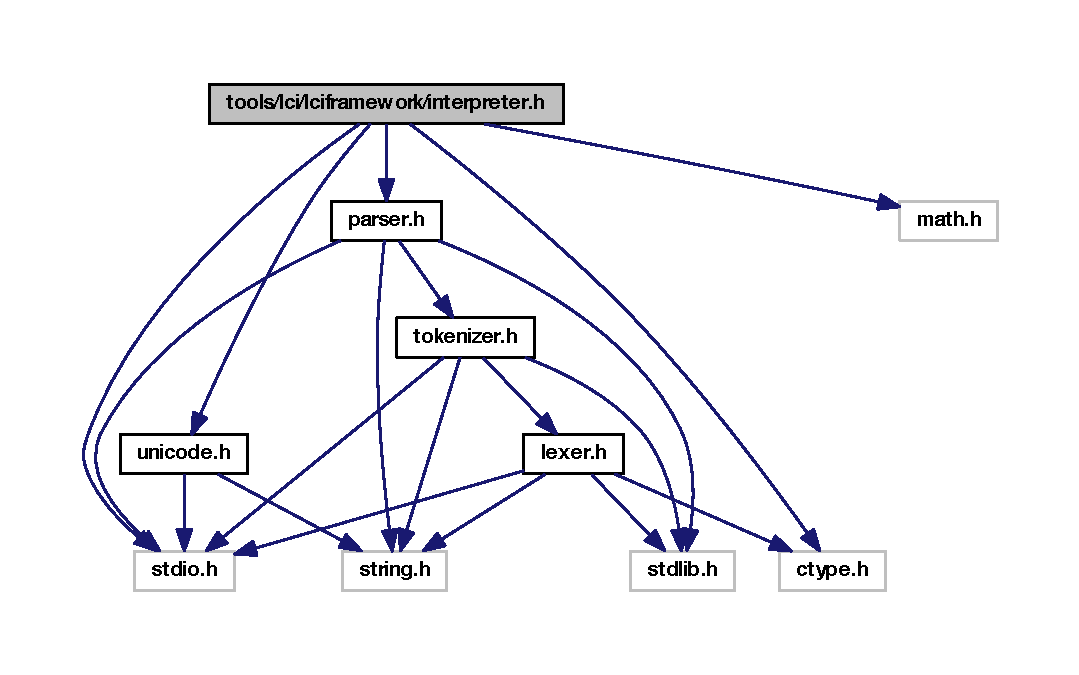
\includegraphics[width=350pt]{interpreter_8h__incl}
\end{center}
\end{figure}
This graph shows which files directly or indirectly include this file\-:
\nopagebreak
\begin{figure}[H]
\begin{center}
\leavevmode
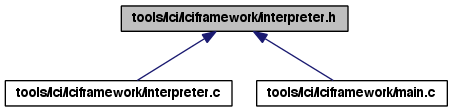
\includegraphics[width=350pt]{interpreter_8h__dep__incl}
\end{center}
\end{figure}
\subsection*{Classes}
\begin{DoxyCompactItemize}
\item 
union \hyperlink{union_value_data}{Value\-Data}
\item 
struct \hyperlink{struct_value_object}{Value\-Object}
\item 
struct \hyperlink{struct_return_object}{Return\-Object}
\item 
struct \hyperlink{structscopeobject}{scopeobject}
\end{DoxyCompactItemize}
\subsection*{Defines}
\begin{DoxyCompactItemize}
\item 
\#define \hyperlink{interpreter_8h_ab09c63bb17c41b5d1c56f89c2a7c0306}{get\-Integer}(value)~(value-\/$>$data.\-i)
\item 
\#define \hyperlink{interpreter_8h_a476129305e12675fd848537c7a23be7e}{get\-Float}(value)~(value-\/$>$data.\-f)
\item 
\#define \hyperlink{interpreter_8h_a2267d4f53f5d3d35446667cc2b26f392}{get\-String}(value)~(value-\/$>$data.\-s)
\item 
\#define \hyperlink{interpreter_8h_acdac0b055f8acfc246c8d1f6cc249012}{V}(value)~(value-\/$>$semaphore++)
\item 
\#define \hyperlink{interpreter_8h_add157945a6056e97010b859dd7b32c2c}{P}(value)~(value-\/$>$semaphore-\/-\/)
\end{DoxyCompactItemize}
\subsection*{Typedefs}
\begin{DoxyCompactItemize}
\item 
typedef struct \hyperlink{structscopeobject}{scopeobject} \hyperlink{interpreter_8h_a7be125c402f07f73bf856b70b37594b5}{Scope\-Object}
\end{DoxyCompactItemize}
\subsection*{Enumerations}
\begin{DoxyCompactItemize}
\item 
enum \hyperlink{interpreter_8h_ad9971b6ef33e02ba2c75d19c1d2518a1}{Value\-Type} \{ \\*
\hyperlink{interpreter_8h_ad9971b6ef33e02ba2c75d19c1d2518a1a656b93fb21c4267dae17573f6129fe93}{V\-T\-\_\-\-I\-N\-T\-E\-G\-E\-R}, 
\hyperlink{interpreter_8h_ad9971b6ef33e02ba2c75d19c1d2518a1a361c0d0ff5ba71f4ddd9633d3f79635f}{V\-T\-\_\-\-F\-L\-O\-A\-T}, 
\hyperlink{interpreter_8h_ad9971b6ef33e02ba2c75d19c1d2518a1aa7db6a14e86242b201db0d4993d61862}{V\-T\-\_\-\-B\-O\-O\-L\-E\-A\-N}, 
\hyperlink{interpreter_8h_ad9971b6ef33e02ba2c75d19c1d2518a1a7d0ada66d85d8eb695f3bdd2e48b5976}{V\-T\-\_\-\-S\-T\-R\-I\-N\-G}, 
\\*
\hyperlink{interpreter_8h_ad9971b6ef33e02ba2c75d19c1d2518a1a523067b7870725372ce9aa1399a8abba}{V\-T\-\_\-\-N\-I\-L}
 \}
\item 
enum \hyperlink{interpreter_8h_a36a419f0b50a0c1d2d4cf712e0ba64cc}{Return\-Type} \{ \hyperlink{interpreter_8h_a36a419f0b50a0c1d2d4cf712e0ba64cca5799e236aeee53b6fe285dc67cb42f00}{R\-T\-\_\-\-D\-E\-F\-A\-U\-L\-T}, 
\hyperlink{interpreter_8h_a36a419f0b50a0c1d2d4cf712e0ba64ccaa22f8c8892450d4ee8806a80a7e12b64}{R\-T\-\_\-\-B\-R\-E\-A\-K}, 
\hyperlink{interpreter_8h_a36a419f0b50a0c1d2d4cf712e0ba64ccae089a7a50c323705d8c848d0308ca41b}{R\-T\-\_\-\-R\-E\-T\-U\-R\-N}
 \}
\end{DoxyCompactItemize}
\subsection*{Functions}
\begin{DoxyCompactItemize}
\item 
char $\ast$ \hyperlink{interpreter_8h_aa775c9107ae005e912e3167801648dee}{create\-String} (char $\ast$)
\item 
\hyperlink{struct_value_object}{Value\-Object} $\ast$ \hyperlink{interpreter_8h_a494ae7c921c6e7994e07d927f1dd619b}{create\-Nil\-Value\-Object} (void)
\item 
\hyperlink{struct_value_object}{Value\-Object} $\ast$ \hyperlink{interpreter_8h_a83170df5413454d013a2624ffde40134}{create\-Boolean\-Value\-Object} (int)
\item 
\hyperlink{struct_value_object}{Value\-Object} $\ast$ \hyperlink{interpreter_8h_a3dcf1ed83c5fe0efe4d7f1c72c023945}{create\-Integer\-Value\-Object} (int)
\item 
\hyperlink{struct_value_object}{Value\-Object} $\ast$ \hyperlink{interpreter_8h_aea96b6d2469b6f3d4531987c644c2d63}{create\-Float\-Value\-Object} (float)
\item 
\hyperlink{struct_value_object}{Value\-Object} $\ast$ \hyperlink{interpreter_8h_a9c7124b50cb92fb20edc6c2963a5f2b8}{create\-String\-Value\-Object} (char $\ast$)
\item 
\hyperlink{struct_value_object}{Value\-Object} $\ast$ \hyperlink{interpreter_8h_a030b889cd6487c903b7e12e69268cdc4}{copy\-Value\-Object} (\hyperlink{struct_value_object}{Value\-Object} $\ast$)
\item 
void \hyperlink{interpreter_8h_a47864225786b36609969a3fea1658a98}{delete\-Value\-Object} (\hyperlink{struct_value_object}{Value\-Object} $\ast$)
\item 
\hyperlink{struct_return_object}{Return\-Object} $\ast$ \hyperlink{interpreter_8h_ae981d9226d812c444fc16aa82755a483}{create\-Return\-Object} (\hyperlink{interpreter_8h_a36a419f0b50a0c1d2d4cf712e0ba64cc}{Return\-Type}, \hyperlink{struct_value_object}{Value\-Object} $\ast$)
\item 
void \hyperlink{interpreter_8h_a573290ef3b6c111b59ad34136dd52d56}{delete\-Return\-Object} (\hyperlink{struct_return_object}{Return\-Object} $\ast$)
\item 
\hyperlink{interpreter_8h_a7be125c402f07f73bf856b70b37594b5}{Scope\-Object} $\ast$ \hyperlink{interpreter_8h_a00f475c904bf21ba3d14fa47177948ff}{create\-Scope\-Object} (\hyperlink{interpreter_8h_a7be125c402f07f73bf856b70b37594b5}{Scope\-Object} $\ast$)
\item 
void \hyperlink{interpreter_8h_a2d477a01d56c2e2aed64ad096c6d5417}{delete\-Scope\-Object} (\hyperlink{interpreter_8h_a7be125c402f07f73bf856b70b37594b5}{Scope\-Object} $\ast$)
\item 
\hyperlink{struct_value_object}{Value\-Object} $\ast$ \hyperlink{interpreter_8h_aad6397fe13daa28d2d902c4f75434360}{get\-Scope\-Value} (\hyperlink{interpreter_8h_a7be125c402f07f73bf856b70b37594b5}{Scope\-Object} $\ast$, \hyperlink{struct_identifier_node}{Identifier\-Node} $\ast$)
\item 
\hyperlink{struct_value_object}{Value\-Object} $\ast$ \hyperlink{interpreter_8h_a6c0c01a1af125b47b7ee6c99a944abb6}{get\-Local\-Scope\-Value} (\hyperlink{interpreter_8h_a7be125c402f07f73bf856b70b37594b5}{Scope\-Object} $\ast$, \hyperlink{struct_identifier_node}{Identifier\-Node} $\ast$)
\item 
\hyperlink{struct_value_object}{Value\-Object} $\ast$ \hyperlink{interpreter_8h_a102e3436ecd759c4504c688b81a8e44a}{create\-Scope\-Value} (\hyperlink{interpreter_8h_a7be125c402f07f73bf856b70b37594b5}{Scope\-Object} $\ast$, \hyperlink{struct_identifier_node}{Identifier\-Node} $\ast$)
\item 
\hyperlink{struct_value_object}{Value\-Object} $\ast$ \hyperlink{interpreter_8h_a8a3976ac7d53fdc0575dfb1cdd2882bc}{update\-Scope\-Value} (\hyperlink{interpreter_8h_a7be125c402f07f73bf856b70b37594b5}{Scope\-Object} $\ast$, \hyperlink{struct_identifier_node}{Identifier\-Node} $\ast$, \hyperlink{struct_value_object}{Value\-Object} $\ast$)
\item 
unsigned int \hyperlink{interpreter_8h_af4fc557b0414d545f179a2eaa80a1a3b}{is\-Num\-String} (const char $\ast$)
\item 
unsigned int \hyperlink{interpreter_8h_a3bcb2030a3649910e8c2f5e073acf436}{is\-Hex\-String} (const char $\ast$)
\item 
\hyperlink{struct_value_object}{Value\-Object} $\ast$ \hyperlink{interpreter_8h_a9da4535836163318aac4d7d2eb03a2d2}{cast\-Boolean\-Explicit} (\hyperlink{struct_value_object}{Value\-Object} $\ast$, \hyperlink{interpreter_8h_a7be125c402f07f73bf856b70b37594b5}{Scope\-Object} $\ast$)
\item 
\hyperlink{struct_value_object}{Value\-Object} $\ast$ \hyperlink{interpreter_8h_aa211d313e27c2f081edc2309a4acb020}{cast\-Integer\-Explicit} (\hyperlink{struct_value_object}{Value\-Object} $\ast$, \hyperlink{interpreter_8h_a7be125c402f07f73bf856b70b37594b5}{Scope\-Object} $\ast$)
\item 
\hyperlink{struct_value_object}{Value\-Object} $\ast$ \hyperlink{interpreter_8h_ab8aff5e3c1456ad85bf55cc816a84a87}{cast\-Float\-Explicit} (\hyperlink{struct_value_object}{Value\-Object} $\ast$, \hyperlink{interpreter_8h_a7be125c402f07f73bf856b70b37594b5}{Scope\-Object} $\ast$)
\item 
\hyperlink{struct_value_object}{Value\-Object} $\ast$ \hyperlink{interpreter_8h_a392cb43c47522cc46d70df0f673b73f6}{cast\-String\-Explicit} (\hyperlink{struct_value_object}{Value\-Object} $\ast$, \hyperlink{interpreter_8h_a7be125c402f07f73bf856b70b37594b5}{Scope\-Object} $\ast$)
\item 
\hyperlink{struct_value_object}{Value\-Object} $\ast$ \hyperlink{interpreter_8h_a17aa2b55578f49903859a41bb1d2dcba}{cast\-Boolean\-Implicit} (\hyperlink{struct_value_object}{Value\-Object} $\ast$, \hyperlink{interpreter_8h_a7be125c402f07f73bf856b70b37594b5}{Scope\-Object} $\ast$)
\item 
\hyperlink{struct_value_object}{Value\-Object} $\ast$ \hyperlink{interpreter_8h_abbf91182fe9db4f0e2e3c4472f0ad431}{cast\-Integer\-Implicit} (\hyperlink{struct_value_object}{Value\-Object} $\ast$, \hyperlink{interpreter_8h_a7be125c402f07f73bf856b70b37594b5}{Scope\-Object} $\ast$)
\item 
\hyperlink{struct_value_object}{Value\-Object} $\ast$ \hyperlink{interpreter_8h_a4132ca66d51545ce6ae5b3287070a50a}{cast\-Float\-Implicit} (\hyperlink{struct_value_object}{Value\-Object} $\ast$, \hyperlink{interpreter_8h_a7be125c402f07f73bf856b70b37594b5}{Scope\-Object} $\ast$)
\item 
\hyperlink{struct_value_object}{Value\-Object} $\ast$ \hyperlink{interpreter_8h_a58e25c56eb8e00ea5b5a2eaca71733b0}{cast\-String\-Implicit} (\hyperlink{struct_value_object}{Value\-Object} $\ast$, \hyperlink{interpreter_8h_a7be125c402f07f73bf856b70b37594b5}{Scope\-Object} $\ast$)
\item 
\hyperlink{struct_value_object}{Value\-Object} $\ast$ \hyperlink{interpreter_8h_a88e238ecbd85b9cfce3d34ad7025774d}{interpret\-Expr\-Node} (\hyperlink{struct_expr_node}{Expr\-Node} $\ast$, \hyperlink{interpreter_8h_a7be125c402f07f73bf856b70b37594b5}{Scope\-Object} $\ast$)
\item 
\hyperlink{struct_return_object}{Return\-Object} $\ast$ \hyperlink{interpreter_8h_a8243b0f033288a08ae06a1fc17c46303}{interpret\-Stmt\-Node} (\hyperlink{struct_stmt_node}{Stmt\-Node} $\ast$, \hyperlink{interpreter_8h_a7be125c402f07f73bf856b70b37594b5}{Scope\-Object} $\ast$)
\item 
\hyperlink{struct_return_object}{Return\-Object} $\ast$ \hyperlink{interpreter_8h_a7bb6c3c2339270c356e1aaaf44c52cf7}{interpret\-Stmt\-Node\-List} (\hyperlink{struct_stmt_node_list}{Stmt\-Node\-List} $\ast$, \hyperlink{interpreter_8h_a7be125c402f07f73bf856b70b37594b5}{Scope\-Object} $\ast$)
\item 
\hyperlink{struct_return_object}{Return\-Object} $\ast$ \hyperlink{interpreter_8h_a35a65f719caa550f2d615abeb26a2200}{interpret\-Block\-Node} (\hyperlink{struct_block_node}{Block\-Node} $\ast$, \hyperlink{interpreter_8h_a7be125c402f07f73bf856b70b37594b5}{Scope\-Object} $\ast$)
\item 
int \hyperlink{interpreter_8h_a30be2c4c505c03683a6a3bdc4f7164aa}{interpret\-Main\-Node} (\hyperlink{struct_main_node}{Main\-Node} $\ast$)
\item 
\hyperlink{struct_value_object}{Value\-Object} $\ast$ \hyperlink{interpreter_8h_a27cedbf17b05209dea5559a175309a14}{interpret\-Imp\-Var\-Expr\-Node} (\hyperlink{struct_expr_node}{Expr\-Node} $\ast$, \hyperlink{interpreter_8h_a7be125c402f07f73bf856b70b37594b5}{Scope\-Object} $\ast$)
\item 
\hyperlink{struct_value_object}{Value\-Object} $\ast$ \hyperlink{interpreter_8h_a8836d5dd711beb5cd96336fe51cdc185}{interpret\-Cast\-Expr\-Node} (\hyperlink{struct_expr_node}{Expr\-Node} $\ast$, \hyperlink{interpreter_8h_a7be125c402f07f73bf856b70b37594b5}{Scope\-Object} $\ast$)
\item 
\hyperlink{struct_value_object}{Value\-Object} $\ast$ \hyperlink{interpreter_8h_aeacd50079f0ce4daf99a11f922182c08}{interpret\-Func\-Call\-Expr\-Node} (\hyperlink{struct_expr_node}{Expr\-Node} $\ast$, \hyperlink{interpreter_8h_a7be125c402f07f73bf856b70b37594b5}{Scope\-Object} $\ast$)
\item 
\hyperlink{struct_value_object}{Value\-Object} $\ast$ \hyperlink{interpreter_8h_a0f42bf997323efdae806c0bcf1c554d8}{interpret\-Identifier\-Expr\-Node} (\hyperlink{struct_expr_node}{Expr\-Node} $\ast$, \hyperlink{interpreter_8h_a7be125c402f07f73bf856b70b37594b5}{Scope\-Object} $\ast$)
\item 
\hyperlink{struct_value_object}{Value\-Object} $\ast$ \hyperlink{interpreter_8h_ad561e8b2aa21983e94b838f30337f099}{interpret\-Constant\-Expr\-Node} (\hyperlink{struct_expr_node}{Expr\-Node} $\ast$, \hyperlink{interpreter_8h_a7be125c402f07f73bf856b70b37594b5}{Scope\-Object} $\ast$)
\item 
\hyperlink{struct_value_object}{Value\-Object} $\ast$ \hyperlink{interpreter_8h_a7795828f9fd573ff3670ade6f6955b07}{interpret\-Not\-Op\-Expr\-Node} (\hyperlink{struct_op_expr_node}{Op\-Expr\-Node} $\ast$, \hyperlink{interpreter_8h_a7be125c402f07f73bf856b70b37594b5}{Scope\-Object} $\ast$)
\item 
\hyperlink{struct_value_object}{Value\-Object} $\ast$ \hyperlink{interpreter_8h_ac43fd9e88414ff9960db8a442ae9a0e8}{interpret\-Arith\-Op\-Expr\-Node} (\hyperlink{struct_op_expr_node}{Op\-Expr\-Node} $\ast$, \hyperlink{interpreter_8h_a7be125c402f07f73bf856b70b37594b5}{Scope\-Object} $\ast$)
\item 
\hyperlink{struct_value_object}{Value\-Object} $\ast$ \hyperlink{interpreter_8h_ad0dc393a1a5f2ef0eb59742fe70f07d1}{interpret\-Bool\-Op\-Expr\-Node} (\hyperlink{struct_op_expr_node}{Op\-Expr\-Node} $\ast$, \hyperlink{interpreter_8h_a7be125c402f07f73bf856b70b37594b5}{Scope\-Object} $\ast$)
\item 
\hyperlink{struct_value_object}{Value\-Object} $\ast$ \hyperlink{interpreter_8h_ab84fa97762a03da8689f763fc3165b41}{interpret\-Equality\-Op\-Expr\-Node} (\hyperlink{struct_op_expr_node}{Op\-Expr\-Node} $\ast$, \hyperlink{interpreter_8h_a7be125c402f07f73bf856b70b37594b5}{Scope\-Object} $\ast$)
\item 
\hyperlink{struct_value_object}{Value\-Object} $\ast$ \hyperlink{interpreter_8h_a4f45d788f390ee7a01a9f7a13f512d03}{interpret\-Concat\-Op\-Expr\-Node} (\hyperlink{struct_op_expr_node}{Op\-Expr\-Node} $\ast$, \hyperlink{interpreter_8h_a7be125c402f07f73bf856b70b37594b5}{Scope\-Object} $\ast$)
\item 
\hyperlink{struct_value_object}{Value\-Object} $\ast$ \hyperlink{interpreter_8h_a14b3a72f8c575160185d3e1ddd9721c3}{interpret\-Op\-Expr\-Node} (\hyperlink{struct_expr_node}{Expr\-Node} $\ast$, \hyperlink{interpreter_8h_a7be125c402f07f73bf856b70b37594b5}{Scope\-Object} $\ast$)
\item 
\hyperlink{struct_return_object}{Return\-Object} $\ast$ \hyperlink{interpreter_8h_a5742a88c672e9e224aecef05663d41ea}{interpret\-Cast\-Stmt\-Node} (\hyperlink{struct_stmt_node}{Stmt\-Node} $\ast$, \hyperlink{interpreter_8h_a7be125c402f07f73bf856b70b37594b5}{Scope\-Object} $\ast$)
\item 
\hyperlink{struct_return_object}{Return\-Object} $\ast$ \hyperlink{interpreter_8h_a3099ebd9282870922a92b1b59f675458}{interpret\-Print\-Stmt\-Node} (\hyperlink{struct_stmt_node}{Stmt\-Node} $\ast$, \hyperlink{interpreter_8h_a7be125c402f07f73bf856b70b37594b5}{Scope\-Object} $\ast$)
\item 
\hyperlink{struct_return_object}{Return\-Object} $\ast$ \hyperlink{interpreter_8h_ababafcbe6b8e86ed3284bb6643baafa4}{interpret\-Input\-Stmt\-Node} (\hyperlink{struct_stmt_node}{Stmt\-Node} $\ast$, \hyperlink{interpreter_8h_a7be125c402f07f73bf856b70b37594b5}{Scope\-Object} $\ast$)
\item 
\hyperlink{struct_return_object}{Return\-Object} $\ast$ \hyperlink{interpreter_8h_a644bee21f70eaa27dd40ae1a9ea07145}{interpret\-Assignment\-Stmt\-Node} (\hyperlink{struct_stmt_node}{Stmt\-Node} $\ast$, \hyperlink{interpreter_8h_a7be125c402f07f73bf856b70b37594b5}{Scope\-Object} $\ast$)
\item 
\hyperlink{struct_return_object}{Return\-Object} $\ast$ \hyperlink{interpreter_8h_a8f688271f7f3ad36ce62428e55940c03}{interpret\-Declaration\-Stmt\-Node} (\hyperlink{struct_stmt_node}{Stmt\-Node} $\ast$, \hyperlink{interpreter_8h_a7be125c402f07f73bf856b70b37594b5}{Scope\-Object} $\ast$)
\item 
\hyperlink{struct_return_object}{Return\-Object} $\ast$ \hyperlink{interpreter_8h_a0214f5c76bcb63a1fbb9a242f9341763}{interpret\-If\-Then\-Else\-Stmt\-Node} (\hyperlink{struct_stmt_node}{Stmt\-Node} $\ast$, \hyperlink{interpreter_8h_a7be125c402f07f73bf856b70b37594b5}{Scope\-Object} $\ast$)
\item 
\hyperlink{struct_return_object}{Return\-Object} $\ast$ \hyperlink{interpreter_8h_acbbc71ff8da84a69bea6a533c73c02ff}{interpret\-Switch\-Stmt\-Node} (\hyperlink{struct_stmt_node}{Stmt\-Node} $\ast$, \hyperlink{interpreter_8h_a7be125c402f07f73bf856b70b37594b5}{Scope\-Object} $\ast$)
\item 
\hyperlink{struct_return_object}{Return\-Object} $\ast$ \hyperlink{interpreter_8h_af8856c962dbaeb39b8a2570c3939bebf}{interpret\-Break\-Stmt\-Node} (\hyperlink{struct_stmt_node}{Stmt\-Node} $\ast$, \hyperlink{interpreter_8h_a7be125c402f07f73bf856b70b37594b5}{Scope\-Object} $\ast$)
\item 
\hyperlink{struct_return_object}{Return\-Object} $\ast$ \hyperlink{interpreter_8h_a83339941f601e7cbbecb09c7501b49fd}{interpret\-Return\-Stmt\-Node} (\hyperlink{struct_stmt_node}{Stmt\-Node} $\ast$, \hyperlink{interpreter_8h_a7be125c402f07f73bf856b70b37594b5}{Scope\-Object} $\ast$)
\item 
\hyperlink{struct_return_object}{Return\-Object} $\ast$ \hyperlink{interpreter_8h_a3907f4b04d219b06c4967b92af485ff8}{interpret\-Loop\-Stmt\-Node} (\hyperlink{struct_stmt_node}{Stmt\-Node} $\ast$, \hyperlink{interpreter_8h_a7be125c402f07f73bf856b70b37594b5}{Scope\-Object} $\ast$)
\item 
\hyperlink{struct_return_object}{Return\-Object} $\ast$ \hyperlink{interpreter_8h_a8760ad4152e9a2dfeb2ed661c3ef04df}{interpret\-Func\-Def\-Stmt\-Node} (\hyperlink{struct_stmt_node}{Stmt\-Node} $\ast$, \hyperlink{interpreter_8h_a7be125c402f07f73bf856b70b37594b5}{Scope\-Object} $\ast$)
\item 
\hyperlink{struct_return_object}{Return\-Object} $\ast$ \hyperlink{interpreter_8h_ab8680118602f725af9bbb28f2a33ba93}{interpret\-Expr\-Stmt\-Node} (\hyperlink{struct_stmt_node}{Stmt\-Node} $\ast$, \hyperlink{interpreter_8h_a7be125c402f07f73bf856b70b37594b5}{Scope\-Object} $\ast$)
\item 
\hyperlink{struct_value_object}{Value\-Object} $\ast$ \hyperlink{interpreter_8h_a60442c44a3ac32b0a98e89294e785c7a}{op\-Add\-Integer\-Integer} (\hyperlink{struct_value_object}{Value\-Object} $\ast$, \hyperlink{struct_value_object}{Value\-Object} $\ast$)
\item 
\hyperlink{struct_value_object}{Value\-Object} $\ast$ \hyperlink{interpreter_8h_a40c15754c7035023570c2f6706aa1bce}{op\-Sub\-Integer\-Integer} (\hyperlink{struct_value_object}{Value\-Object} $\ast$, \hyperlink{struct_value_object}{Value\-Object} $\ast$)
\item 
\hyperlink{struct_value_object}{Value\-Object} $\ast$ \hyperlink{interpreter_8h_a49439f8122d53198698d46dc8e355dec}{op\-Mult\-Integer\-Integer} (\hyperlink{struct_value_object}{Value\-Object} $\ast$, \hyperlink{struct_value_object}{Value\-Object} $\ast$)
\item 
\hyperlink{struct_value_object}{Value\-Object} $\ast$ \hyperlink{interpreter_8h_a1c2bad8d59cc55d1de2e90818552b727}{op\-Div\-Integer\-Integer} (\hyperlink{struct_value_object}{Value\-Object} $\ast$, \hyperlink{struct_value_object}{Value\-Object} $\ast$)
\item 
\hyperlink{struct_value_object}{Value\-Object} $\ast$ \hyperlink{interpreter_8h_a60d738376880221327c82bb0bf2de141}{op\-Max\-Integer\-Integer} (\hyperlink{struct_value_object}{Value\-Object} $\ast$, \hyperlink{struct_value_object}{Value\-Object} $\ast$)
\item 
\hyperlink{struct_value_object}{Value\-Object} $\ast$ \hyperlink{interpreter_8h_af3f2a6f50fdd068834ab1b58d4928ec8}{op\-Min\-Integer\-Integer} (\hyperlink{struct_value_object}{Value\-Object} $\ast$, \hyperlink{struct_value_object}{Value\-Object} $\ast$)
\item 
\hyperlink{struct_value_object}{Value\-Object} $\ast$ \hyperlink{interpreter_8h_a87b62a374250d0fbe4e9e95497c10b15}{op\-Mod\-Integer\-Integer} (\hyperlink{struct_value_object}{Value\-Object} $\ast$, \hyperlink{struct_value_object}{Value\-Object} $\ast$)
\item 
\hyperlink{struct_value_object}{Value\-Object} $\ast$ \hyperlink{interpreter_8h_afd694eb2626213010cbc38830a462fde}{op\-Add\-Integer\-Float} (\hyperlink{struct_value_object}{Value\-Object} $\ast$, \hyperlink{struct_value_object}{Value\-Object} $\ast$)
\item 
\hyperlink{struct_value_object}{Value\-Object} $\ast$ \hyperlink{interpreter_8h_a305d078f6079ca2938e21409816000be}{op\-Sub\-Integer\-Float} (\hyperlink{struct_value_object}{Value\-Object} $\ast$, \hyperlink{struct_value_object}{Value\-Object} $\ast$)
\item 
\hyperlink{struct_value_object}{Value\-Object} $\ast$ \hyperlink{interpreter_8h_a5393045000bf05070b764eebe2012627}{op\-Mult\-Integer\-Float} (\hyperlink{struct_value_object}{Value\-Object} $\ast$, \hyperlink{struct_value_object}{Value\-Object} $\ast$)
\item 
\hyperlink{struct_value_object}{Value\-Object} $\ast$ \hyperlink{interpreter_8h_a0df5be521bfc67b35aca6ab1e30c2a32}{op\-Div\-Integer\-Float} (\hyperlink{struct_value_object}{Value\-Object} $\ast$, \hyperlink{struct_value_object}{Value\-Object} $\ast$)
\item 
\hyperlink{struct_value_object}{Value\-Object} $\ast$ \hyperlink{interpreter_8h_a5d68c3dc91195706810b6db725e62eaa}{op\-Max\-Integer\-Float} (\hyperlink{struct_value_object}{Value\-Object} $\ast$, \hyperlink{struct_value_object}{Value\-Object} $\ast$)
\item 
\hyperlink{struct_value_object}{Value\-Object} $\ast$ \hyperlink{interpreter_8h_a5693ec134e9b9090f8cfe51d9906e38e}{op\-Min\-Integer\-Float} (\hyperlink{struct_value_object}{Value\-Object} $\ast$, \hyperlink{struct_value_object}{Value\-Object} $\ast$)
\item 
\hyperlink{struct_value_object}{Value\-Object} $\ast$ \hyperlink{interpreter_8h_a6fa3fda306a1df48dfe9fbc2cff75d74}{op\-Mod\-Integer\-Float} (\hyperlink{struct_value_object}{Value\-Object} $\ast$, \hyperlink{struct_value_object}{Value\-Object} $\ast$)
\item 
\hyperlink{struct_value_object}{Value\-Object} $\ast$ \hyperlink{interpreter_8h_a7c2619ce0699c09c53ab2aaf2c0977f7}{op\-Add\-Float\-Integer} (\hyperlink{struct_value_object}{Value\-Object} $\ast$, \hyperlink{struct_value_object}{Value\-Object} $\ast$)
\item 
\hyperlink{struct_value_object}{Value\-Object} $\ast$ \hyperlink{interpreter_8h_a499e486ea1a832b7105d3d8da3b76e91}{op\-Sub\-Float\-Integer} (\hyperlink{struct_value_object}{Value\-Object} $\ast$, \hyperlink{struct_value_object}{Value\-Object} $\ast$)
\item 
\hyperlink{struct_value_object}{Value\-Object} $\ast$ \hyperlink{interpreter_8h_a2cae8b697111b4eea690cdd38ddbc5a8}{op\-Mult\-Float\-Integer} (\hyperlink{struct_value_object}{Value\-Object} $\ast$, \hyperlink{struct_value_object}{Value\-Object} $\ast$)
\item 
\hyperlink{struct_value_object}{Value\-Object} $\ast$ \hyperlink{interpreter_8h_a89ec3da04bba6b628f84b131e804e3aa}{op\-Div\-Float\-Integer} (\hyperlink{struct_value_object}{Value\-Object} $\ast$, \hyperlink{struct_value_object}{Value\-Object} $\ast$)
\item 
\hyperlink{struct_value_object}{Value\-Object} $\ast$ \hyperlink{interpreter_8h_ae290f0012a6e7ac888f6e42e162db0d1}{op\-Max\-Float\-Integer} (\hyperlink{struct_value_object}{Value\-Object} $\ast$, \hyperlink{struct_value_object}{Value\-Object} $\ast$)
\item 
\hyperlink{struct_value_object}{Value\-Object} $\ast$ \hyperlink{interpreter_8h_aeba04e12530543d1ecc8a70669fac094}{op\-Min\-Float\-Integer} (\hyperlink{struct_value_object}{Value\-Object} $\ast$, \hyperlink{struct_value_object}{Value\-Object} $\ast$)
\item 
\hyperlink{struct_value_object}{Value\-Object} $\ast$ \hyperlink{interpreter_8h_a6d90cdaea27748de7784f43f82c31c8a}{op\-Mod\-Float\-Integer} (\hyperlink{struct_value_object}{Value\-Object} $\ast$, \hyperlink{struct_value_object}{Value\-Object} $\ast$)
\item 
\hyperlink{struct_value_object}{Value\-Object} $\ast$ \hyperlink{interpreter_8h_ad07ed5a492963cbbfbaf26f10178a0da}{op\-Add\-Float\-Float} (\hyperlink{struct_value_object}{Value\-Object} $\ast$, \hyperlink{struct_value_object}{Value\-Object} $\ast$)
\item 
\hyperlink{struct_value_object}{Value\-Object} $\ast$ \hyperlink{interpreter_8h_a6fe0baa044b43505a5013455ce7f3ef4}{op\-Sub\-Float\-Float} (\hyperlink{struct_value_object}{Value\-Object} $\ast$, \hyperlink{struct_value_object}{Value\-Object} $\ast$)
\item 
\hyperlink{struct_value_object}{Value\-Object} $\ast$ \hyperlink{interpreter_8h_ab28d564ef0da5903a3a2ed6c18dcad11}{op\-Mult\-Float\-Float} (\hyperlink{struct_value_object}{Value\-Object} $\ast$, \hyperlink{struct_value_object}{Value\-Object} $\ast$)
\item 
\hyperlink{struct_value_object}{Value\-Object} $\ast$ \hyperlink{interpreter_8h_a907454143b8856fe616d3b595cb917d1}{op\-Div\-Float\-Float} (\hyperlink{struct_value_object}{Value\-Object} $\ast$, \hyperlink{struct_value_object}{Value\-Object} $\ast$)
\item 
\hyperlink{struct_value_object}{Value\-Object} $\ast$ \hyperlink{interpreter_8h_a744d79a234d2a4f6490ef91624071c32}{op\-Max\-Float\-Float} (\hyperlink{struct_value_object}{Value\-Object} $\ast$, \hyperlink{struct_value_object}{Value\-Object} $\ast$)
\item 
\hyperlink{struct_value_object}{Value\-Object} $\ast$ \hyperlink{interpreter_8h_a901fca3f0217cce10f23a893372680a8}{op\-Min\-Float\-Float} (\hyperlink{struct_value_object}{Value\-Object} $\ast$, \hyperlink{struct_value_object}{Value\-Object} $\ast$)
\item 
\hyperlink{struct_value_object}{Value\-Object} $\ast$ \hyperlink{interpreter_8h_ae7fd86387767d294c071b020ea5e9ccc}{op\-Mod\-Float\-Float} (\hyperlink{struct_value_object}{Value\-Object} $\ast$, \hyperlink{struct_value_object}{Value\-Object} $\ast$)
\item 
\hyperlink{struct_value_object}{Value\-Object} $\ast$ \hyperlink{interpreter_8h_a49a410f97c8559f2ba41ca94b7aceb21}{op\-Eq\-Boolean\-Boolean} (\hyperlink{struct_value_object}{Value\-Object} $\ast$, \hyperlink{struct_value_object}{Value\-Object} $\ast$)
\item 
\hyperlink{struct_value_object}{Value\-Object} $\ast$ \hyperlink{interpreter_8h_adf2234eccc6099f2f1829a7ee948e045}{op\-Neq\-Boolean\-Boolean} (\hyperlink{struct_value_object}{Value\-Object} $\ast$, \hyperlink{struct_value_object}{Value\-Object} $\ast$)
\item 
\hyperlink{struct_value_object}{Value\-Object} $\ast$ \hyperlink{interpreter_8h_af02dbffb1883def8d565b324d3b08fa4}{op\-Eq\-Integer\-Integer} (\hyperlink{struct_value_object}{Value\-Object} $\ast$, \hyperlink{struct_value_object}{Value\-Object} $\ast$)
\item 
\hyperlink{struct_value_object}{Value\-Object} $\ast$ \hyperlink{interpreter_8h_a737fac56d37cbf193f78775774cfdeeb}{op\-Neq\-Integer\-Integer} (\hyperlink{struct_value_object}{Value\-Object} $\ast$, \hyperlink{struct_value_object}{Value\-Object} $\ast$)
\item 
\hyperlink{struct_value_object}{Value\-Object} $\ast$ \hyperlink{interpreter_8h_a918c1fe2753f0fa6a7f0abbb0f26790f}{op\-Eq\-Integer\-Float} (\hyperlink{struct_value_object}{Value\-Object} $\ast$, \hyperlink{struct_value_object}{Value\-Object} $\ast$)
\item 
\hyperlink{struct_value_object}{Value\-Object} $\ast$ \hyperlink{interpreter_8h_a689189c68d9b98c49d296cd9f04363e9}{op\-Neq\-Integer\-Float} (\hyperlink{struct_value_object}{Value\-Object} $\ast$, \hyperlink{struct_value_object}{Value\-Object} $\ast$)
\item 
\hyperlink{struct_value_object}{Value\-Object} $\ast$ \hyperlink{interpreter_8h_a5b824e009801b5ca65d51abe36aecf97}{op\-Eq\-Float\-Integer} (\hyperlink{struct_value_object}{Value\-Object} $\ast$, \hyperlink{struct_value_object}{Value\-Object} $\ast$)
\item 
\hyperlink{struct_value_object}{Value\-Object} $\ast$ \hyperlink{interpreter_8h_a48ab7e79793cd6462d041d6288b770d9}{op\-Neq\-Float\-Integer} (\hyperlink{struct_value_object}{Value\-Object} $\ast$, \hyperlink{struct_value_object}{Value\-Object} $\ast$)
\item 
\hyperlink{struct_value_object}{Value\-Object} $\ast$ \hyperlink{interpreter_8h_ab721f724a3fac4900c4a8886d57c41d2}{op\-Eq\-Float\-Float} (\hyperlink{struct_value_object}{Value\-Object} $\ast$, \hyperlink{struct_value_object}{Value\-Object} $\ast$)
\item 
\hyperlink{struct_value_object}{Value\-Object} $\ast$ \hyperlink{interpreter_8h_ac2f5e5a62a09a571b8be1ab942fa29cd}{op\-Neq\-Float\-Float} (\hyperlink{struct_value_object}{Value\-Object} $\ast$, \hyperlink{struct_value_object}{Value\-Object} $\ast$)
\item 
\hyperlink{struct_value_object}{Value\-Object} $\ast$ \hyperlink{interpreter_8h_a990ba01ec898389b6bde8471e2ad0f9d}{op\-Eq\-String\-String} (\hyperlink{struct_value_object}{Value\-Object} $\ast$, \hyperlink{struct_value_object}{Value\-Object} $\ast$)
\item 
\hyperlink{struct_value_object}{Value\-Object} $\ast$ \hyperlink{interpreter_8h_a207c76cef3c01faa73750bd60e9b0037}{op\-Neq\-String\-String} (\hyperlink{struct_value_object}{Value\-Object} $\ast$, \hyperlink{struct_value_object}{Value\-Object} $\ast$)
\item 
\hyperlink{struct_value_object}{Value\-Object} $\ast$ \hyperlink{interpreter_8h_aa910b7104ad75428e66766f5bd06f4a8}{op\-Eq\-Nil\-Nil} (\hyperlink{struct_value_object}{Value\-Object} $\ast$, \hyperlink{struct_value_object}{Value\-Object} $\ast$)
\item 
\hyperlink{struct_value_object}{Value\-Object} $\ast$ \hyperlink{interpreter_8h_a7ad8e455aa33ebc978836eab51b9c268}{op\-Neq\-Nil\-Nil} (\hyperlink{struct_value_object}{Value\-Object} $\ast$, \hyperlink{struct_value_object}{Value\-Object} $\ast$)
\end{DoxyCompactItemize}


\subsection{Detailed Description}
Structures and functions for interpreting a parse tree. The interpreter traverses a parse tree in a depth-\/first manner, interpreting each node it reaches along the way. This is the last stage of the processing of a source code file.

\begin{DoxyAuthor}{Author}
Justin J. Meza
\end{DoxyAuthor}
\begin{DoxyDate}{Date}
2010 
\end{DoxyDate}


Definition in file \hyperlink{interpreter_8h_source}{interpreter.\-h}.



\subsection{Define Documentation}
\hypertarget{interpreter_8h_a476129305e12675fd848537c7a23be7e}{\index{interpreter.\-h@{interpreter.\-h}!get\-Float@{get\-Float}}
\index{get\-Float@{get\-Float}!interpreter.h@{interpreter.\-h}}
\subsubsection[{get\-Float}]{\setlength{\rightskip}{0pt plus 5cm}\#define {\bf get\-Float}(
\begin{DoxyParamCaption}
\item[{}]{value}
\end{DoxyParamCaption}
)~(value-\/$>$data.\-f)}}\label{interpreter_8h_a476129305e12675fd848537c7a23be7e}
Gets the floating point data associated with a \hyperlink{struct_value_object}{Value\-Object} structure. 

Definition at line 25 of file interpreter.\-h.

\hypertarget{interpreter_8h_ab09c63bb17c41b5d1c56f89c2a7c0306}{\index{interpreter.\-h@{interpreter.\-h}!get\-Integer@{get\-Integer}}
\index{get\-Integer@{get\-Integer}!interpreter.h@{interpreter.\-h}}
\subsubsection[{get\-Integer}]{\setlength{\rightskip}{0pt plus 5cm}\#define {\bf get\-Integer}(
\begin{DoxyParamCaption}
\item[{}]{value}
\end{DoxyParamCaption}
)~(value-\/$>$data.\-i)}}\label{interpreter_8h_ab09c63bb17c41b5d1c56f89c2a7c0306}
Gets the integer data associated with a \hyperlink{struct_value_object}{Value\-Object} structure. 

Definition at line 23 of file interpreter.\-h.

\hypertarget{interpreter_8h_a2267d4f53f5d3d35446667cc2b26f392}{\index{interpreter.\-h@{interpreter.\-h}!get\-String@{get\-String}}
\index{get\-String@{get\-String}!interpreter.h@{interpreter.\-h}}
\subsubsection[{get\-String}]{\setlength{\rightskip}{0pt plus 5cm}\#define {\bf get\-String}(
\begin{DoxyParamCaption}
\item[{}]{value}
\end{DoxyParamCaption}
)~(value-\/$>$data.\-s)}}\label{interpreter_8h_a2267d4f53f5d3d35446667cc2b26f392}
Gets the string data associated with a \hyperlink{struct_value_object}{Value\-Object} structure. 

Definition at line 27 of file interpreter.\-h.

\hypertarget{interpreter_8h_add157945a6056e97010b859dd7b32c2c}{\index{interpreter.\-h@{interpreter.\-h}!P@{P}}
\index{P@{P}!interpreter.h@{interpreter.\-h}}
\subsubsection[{P}]{\setlength{\rightskip}{0pt plus 5cm}\#define {\bf P}(
\begin{DoxyParamCaption}
\item[{}]{value}
\end{DoxyParamCaption}
)~(value-\/$>$semaphore-\/-\/)}}\label{interpreter_8h_add157945a6056e97010b859dd7b32c2c}
Decrements the semaphore of a \hyperlink{struct_value_object}{Value\-Object} structure. 

Definition at line 49 of file interpreter.\-h.

\hypertarget{interpreter_8h_acdac0b055f8acfc246c8d1f6cc249012}{\index{interpreter.\-h@{interpreter.\-h}!V@{V}}
\index{V@{V}!interpreter.h@{interpreter.\-h}}
\subsubsection[{V}]{\setlength{\rightskip}{0pt plus 5cm}\#define {\bf V}(
\begin{DoxyParamCaption}
\item[{}]{value}
\end{DoxyParamCaption}
)~(value-\/$>$semaphore++)}}\label{interpreter_8h_acdac0b055f8acfc246c8d1f6cc249012}
Increments the semaphore of a \hyperlink{struct_value_object}{Value\-Object} structure. 

Definition at line 46 of file interpreter.\-h.



\subsection{Typedef Documentation}
\hypertarget{interpreter_8h_a7be125c402f07f73bf856b70b37594b5}{\index{interpreter.\-h@{interpreter.\-h}!Scope\-Object@{Scope\-Object}}
\index{Scope\-Object@{Scope\-Object}!interpreter.h@{interpreter.\-h}}
\subsubsection[{Scope\-Object}]{\setlength{\rightskip}{0pt plus 5cm}typedef struct {\bf scopeobject}  {\bf Scope\-Object}}}\label{interpreter_8h_a7be125c402f07f73bf856b70b37594b5}
Stores the variables in a particular scope. Scopes are arranged heirarchically from global (the ancestor of all other scopes) to local (the temporary scope of a \hyperlink{struct_block_node}{Block\-Node}).

\begin{DoxySeeAlso}{See also}
\hyperlink{interpreter_8h_a00f475c904bf21ba3d14fa47177948ff}{create\-Scope\-Object(\-Scope\-Object $\ast$)} 

\hyperlink{interpreter_8h_a2d477a01d56c2e2aed64ad096c6d5417}{delete\-Scope\-Object(\-Scope\-Object $\ast$)} 
\end{DoxySeeAlso}


\subsection{Enumeration Type Documentation}
\hypertarget{interpreter_8h_a36a419f0b50a0c1d2d4cf712e0ba64cc}{\index{interpreter.\-h@{interpreter.\-h}!Return\-Type@{Return\-Type}}
\index{Return\-Type@{Return\-Type}!interpreter.h@{interpreter.\-h}}
\subsubsection[{Return\-Type}]{\setlength{\rightskip}{0pt plus 5cm}enum {\bf Return\-Type}}}\label{interpreter_8h_a36a419f0b50a0c1d2d4cf712e0ba64cc}
Denotes the type of return encountered. \begin{Desc}
\item[Enumerator\-: ]\par
\begin{description}
\index{R\-T\-\_\-\-D\-E\-F\-A\-U\-L\-T@{R\-T\-\_\-\-D\-E\-F\-A\-U\-L\-T}!interpreter.\-h@{interpreter.\-h}}\index{interpreter.\-h@{interpreter.\-h}!R\-T\-\_\-\-D\-E\-F\-A\-U\-L\-T@{R\-T\-\_\-\-D\-E\-F\-A\-U\-L\-T}}\item[{\em 
\hypertarget{interpreter_8h_a36a419f0b50a0c1d2d4cf712e0ba64cca5799e236aeee53b6fe285dc67cb42f00}{R\-T\-\_\-\-D\-E\-F\-A\-U\-L\-T}\label{interpreter_8h_a36a419f0b50a0c1d2d4cf712e0ba64cca5799e236aeee53b6fe285dc67cb42f00}
}]A block of code returned after evaluating all of its statements. \index{R\-T\-\_\-\-B\-R\-E\-A\-K@{R\-T\-\_\-\-B\-R\-E\-A\-K}!interpreter.\-h@{interpreter.\-h}}\index{interpreter.\-h@{interpreter.\-h}!R\-T\-\_\-\-B\-R\-E\-A\-K@{R\-T\-\_\-\-B\-R\-E\-A\-K}}\item[{\em 
\hypertarget{interpreter_8h_a36a419f0b50a0c1d2d4cf712e0ba64ccaa22f8c8892450d4ee8806a80a7e12b64}{R\-T\-\_\-\-B\-R\-E\-A\-K}\label{interpreter_8h_a36a419f0b50a0c1d2d4cf712e0ba64ccaa22f8c8892450d4ee8806a80a7e12b64}
}]A block of code within a \hyperlink{struct_loop_stmt_node}{Loop\-Stmt\-Node} or \hyperlink{struct_switch_stmt_node}{Switch\-Stmt\-Node} returned via a break statement. \index{R\-T\-\_\-\-R\-E\-T\-U\-R\-N@{R\-T\-\_\-\-R\-E\-T\-U\-R\-N}!interpreter.\-h@{interpreter.\-h}}\index{interpreter.\-h@{interpreter.\-h}!R\-T\-\_\-\-R\-E\-T\-U\-R\-N@{R\-T\-\_\-\-R\-E\-T\-U\-R\-N}}\item[{\em 
\hypertarget{interpreter_8h_a36a419f0b50a0c1d2d4cf712e0ba64ccae089a7a50c323705d8c848d0308ca41b}{R\-T\-\_\-\-R\-E\-T\-U\-R\-N}\label{interpreter_8h_a36a419f0b50a0c1d2d4cf712e0ba64ccae089a7a50c323705d8c848d0308ca41b}
}]A block of code within a \hyperlink{struct_func_def_stmt_node}{Func\-Def\-Stmt\-Node} called by a \hyperlink{struct_func_call_expr_node}{Func\-Call\-Expr\-Node} returned (either with or without a value). \end{description}
\end{Desc}



Definition at line 62 of file interpreter.\-h.

\hypertarget{interpreter_8h_ad9971b6ef33e02ba2c75d19c1d2518a1}{\index{interpreter.\-h@{interpreter.\-h}!Value\-Type@{Value\-Type}}
\index{Value\-Type@{Value\-Type}!interpreter.h@{interpreter.\-h}}
\subsubsection[{Value\-Type}]{\setlength{\rightskip}{0pt plus 5cm}enum {\bf Value\-Type}}}\label{interpreter_8h_ad9971b6ef33e02ba2c75d19c1d2518a1}
Denotes the type of a value. \begin{Desc}
\item[Enumerator\-: ]\par
\begin{description}
\index{V\-T\-\_\-\-I\-N\-T\-E\-G\-E\-R@{V\-T\-\_\-\-I\-N\-T\-E\-G\-E\-R}!interpreter.\-h@{interpreter.\-h}}\index{interpreter.\-h@{interpreter.\-h}!V\-T\-\_\-\-I\-N\-T\-E\-G\-E\-R@{V\-T\-\_\-\-I\-N\-T\-E\-G\-E\-R}}\item[{\em 
\hypertarget{interpreter_8h_ad9971b6ef33e02ba2c75d19c1d2518a1a656b93fb21c4267dae17573f6129fe93}{V\-T\-\_\-\-I\-N\-T\-E\-G\-E\-R}\label{interpreter_8h_ad9971b6ef33e02ba2c75d19c1d2518a1a656b93fb21c4267dae17573f6129fe93}
}]An integer value. \index{V\-T\-\_\-\-F\-L\-O\-A\-T@{V\-T\-\_\-\-F\-L\-O\-A\-T}!interpreter.\-h@{interpreter.\-h}}\index{interpreter.\-h@{interpreter.\-h}!V\-T\-\_\-\-F\-L\-O\-A\-T@{V\-T\-\_\-\-F\-L\-O\-A\-T}}\item[{\em 
\hypertarget{interpreter_8h_ad9971b6ef33e02ba2c75d19c1d2518a1a361c0d0ff5ba71f4ddd9633d3f79635f}{V\-T\-\_\-\-F\-L\-O\-A\-T}\label{interpreter_8h_ad9971b6ef33e02ba2c75d19c1d2518a1a361c0d0ff5ba71f4ddd9633d3f79635f}
}]A floating point decimal value. \index{V\-T\-\_\-\-B\-O\-O\-L\-E\-A\-N@{V\-T\-\_\-\-B\-O\-O\-L\-E\-A\-N}!interpreter.\-h@{interpreter.\-h}}\index{interpreter.\-h@{interpreter.\-h}!V\-T\-\_\-\-B\-O\-O\-L\-E\-A\-N@{V\-T\-\_\-\-B\-O\-O\-L\-E\-A\-N}}\item[{\em 
\hypertarget{interpreter_8h_ad9971b6ef33e02ba2c75d19c1d2518a1aa7db6a14e86242b201db0d4993d61862}{V\-T\-\_\-\-B\-O\-O\-L\-E\-A\-N}\label{interpreter_8h_ad9971b6ef33e02ba2c75d19c1d2518a1aa7db6a14e86242b201db0d4993d61862}
}]A true/false value. \index{V\-T\-\_\-\-S\-T\-R\-I\-N\-G@{V\-T\-\_\-\-S\-T\-R\-I\-N\-G}!interpreter.\-h@{interpreter.\-h}}\index{interpreter.\-h@{interpreter.\-h}!V\-T\-\_\-\-S\-T\-R\-I\-N\-G@{V\-T\-\_\-\-S\-T\-R\-I\-N\-G}}\item[{\em 
\hypertarget{interpreter_8h_ad9971b6ef33e02ba2c75d19c1d2518a1a7d0ada66d85d8eb695f3bdd2e48b5976}{V\-T\-\_\-\-S\-T\-R\-I\-N\-G}\label{interpreter_8h_ad9971b6ef33e02ba2c75d19c1d2518a1a7d0ada66d85d8eb695f3bdd2e48b5976}
}]A character string value. \index{V\-T\-\_\-\-N\-I\-L@{V\-T\-\_\-\-N\-I\-L}!interpreter.\-h@{interpreter.\-h}}\index{interpreter.\-h@{interpreter.\-h}!V\-T\-\_\-\-N\-I\-L@{V\-T\-\_\-\-N\-I\-L}}\item[{\em 
\hypertarget{interpreter_8h_ad9971b6ef33e02ba2c75d19c1d2518a1a523067b7870725372ce9aa1399a8abba}{V\-T\-\_\-\-N\-I\-L}\label{interpreter_8h_ad9971b6ef33e02ba2c75d19c1d2518a1a523067b7870725372ce9aa1399a8abba}
}]Represents no value. \end{description}
\end{Desc}



Definition at line 30 of file interpreter.\-h.



\subsection{Function Documentation}
\hypertarget{interpreter_8h_a9da4535836163318aac4d7d2eb03a2d2}{\index{interpreter.\-h@{interpreter.\-h}!cast\-Boolean\-Explicit@{cast\-Boolean\-Explicit}}
\index{cast\-Boolean\-Explicit@{cast\-Boolean\-Explicit}!interpreter.h@{interpreter.\-h}}
\subsubsection[{cast\-Boolean\-Explicit}]{\setlength{\rightskip}{0pt plus 5cm}{\bf Value\-Object}$\ast$ {\bf cast\-Boolean\-Explicit} (
\begin{DoxyParamCaption}
\item[{{\bf Value\-Object} $\ast$}]{node, }
\item[{{\bf Scope\-Object} $\ast$}]{scope}
\end{DoxyParamCaption}
)}}\label{interpreter_8h_a9da4535836163318aac4d7d2eb03a2d2}
Casts the contents of a \hyperlink{struct_value_object}{Value\-Object} structure to boolean type in an explicit context. Casting is not done directly to the \hyperlink{struct_value_object}{Value\-Object} structure pointed to by {\itshape node\/}, instead, it is performed on a copy of that structure, which is what is returned.

\begin{DoxyPrecond}{Precondition}
{\itshape node\/} was created by either \hyperlink{interpreter_8h_a494ae7c921c6e7994e07d927f1dd619b}{create\-Nil\-Value\-Object(void)}, \hyperlink{interpreter_8h_a83170df5413454d013a2624ffde40134}{create\-Boolean\-Value\-Object(int)}, \hyperlink{interpreter_8h_a3dcf1ed83c5fe0efe4d7f1c72c023945}{create\-Integer\-Value\-Object(int)}, \hyperlink{interpreter_8h_aea96b6d2469b6f3d4531987c644c2d63}{create\-Float\-Value\-Object(float)}, \hyperlink{interpreter_8h_a9c7124b50cb92fb20edc6c2963a5f2b8}{create\-String\-Value\-Object(char $\ast$)}, or copied with \hyperlink{interpreter_8h_a030b889cd6487c903b7e12e69268cdc4}{copy\-Value\-Object(\-Value\-Object $\ast$)}. 

{\itshape scope\/} was created by \hyperlink{interpreter_8h_a00f475c904bf21ba3d14fa47177948ff}{create\-Scope\-Object(\-Scope\-Object $\ast$)}.
\end{DoxyPrecond}
\begin{DoxyReturn}{Returns}
A pointer to a \hyperlink{struct_value_object}{Value\-Object} structure with a copy of the contents of {\itshape node\/}, cast to boolean type.
\end{DoxyReturn}

\begin{DoxyRetVals}{Return values}
{\em N\-U\-L\-L} & An error occurred while casting.\\
\hline
\end{DoxyRetVals}
\begin{DoxySeeAlso}{See also}
\hyperlink{interpreter_8h_aa211d313e27c2f081edc2309a4acb020}{cast\-Integer\-Explicit(\-Value\-Object $\ast$, Scope\-Object $\ast$)} 

\hyperlink{interpreter_8h_ab8aff5e3c1456ad85bf55cc816a84a87}{cast\-Float\-Explicit(\-Value\-Object $\ast$, Scope\-Object $\ast$)} 

\hyperlink{interpreter_8h_a392cb43c47522cc46d70df0f673b73f6}{cast\-String\-Explicit(\-Value\-Object $\ast$, Scope\-Object $\ast$)} 
\end{DoxySeeAlso}

\begin{DoxyParams}[1]{Parameters}
\mbox{\tt in}  & {\em node} & The \hyperlink{struct_value_object}{Value\-Object} structure to cast. \\
\hline
\mbox{\tt in}  & {\em scope} & The Scope\-Object structure to use for variable interpolation. \\
\hline
\end{DoxyParams}


Definition at line 600 of file interpreter.\-c.

\hypertarget{interpreter_8h_a17aa2b55578f49903859a41bb1d2dcba}{\index{interpreter.\-h@{interpreter.\-h}!cast\-Boolean\-Implicit@{cast\-Boolean\-Implicit}}
\index{cast\-Boolean\-Implicit@{cast\-Boolean\-Implicit}!interpreter.h@{interpreter.\-h}}
\subsubsection[{cast\-Boolean\-Implicit}]{\setlength{\rightskip}{0pt plus 5cm}{\bf Value\-Object}$\ast$ {\bf cast\-Boolean\-Implicit} (
\begin{DoxyParamCaption}
\item[{{\bf Value\-Object} $\ast$}]{node, }
\item[{{\bf Scope\-Object} $\ast$}]{scope}
\end{DoxyParamCaption}
)}}\label{interpreter_8h_a17aa2b55578f49903859a41bb1d2dcba}
Casts the contents of a \hyperlink{struct_value_object}{Value\-Object} structure to boolean type in an implicit context. Casting is not done directly to the \hyperlink{struct_value_object}{Value\-Object} structure pointed to by {\itshape node\/}, instead, it is performed on a copy of that structure, which is what is returned.

\begin{DoxyPrecond}{Precondition}
{\itshape node\/} was created by either \hyperlink{interpreter_8h_a494ae7c921c6e7994e07d927f1dd619b}{create\-Nil\-Value\-Object(void)}, \hyperlink{interpreter_8h_a83170df5413454d013a2624ffde40134}{create\-Boolean\-Value\-Object(int)}, \hyperlink{interpreter_8h_a3dcf1ed83c5fe0efe4d7f1c72c023945}{create\-Integer\-Value\-Object(int)}, \hyperlink{interpreter_8h_aea96b6d2469b6f3d4531987c644c2d63}{create\-Float\-Value\-Object(float)}, \hyperlink{interpreter_8h_a9c7124b50cb92fb20edc6c2963a5f2b8}{create\-String\-Value\-Object(char $\ast$)}, or copied with \hyperlink{interpreter_8h_a030b889cd6487c903b7e12e69268cdc4}{copy\-Value\-Object(\-Value\-Object $\ast$)}. 

{\itshape scope\/} was created by \hyperlink{interpreter_8h_a00f475c904bf21ba3d14fa47177948ff}{create\-Scope\-Object(\-Scope\-Object $\ast$)}.
\end{DoxyPrecond}
\begin{DoxyReturn}{Returns}
A pointer to a \hyperlink{struct_value_object}{Value\-Object} structure with a copy of the contents of {\itshape node\/}, cast to boolean type.
\end{DoxyReturn}

\begin{DoxyRetVals}{Return values}
{\em N\-U\-L\-L} & An error occurred while casting.\\
\hline
\end{DoxyRetVals}
\begin{DoxySeeAlso}{See also}
\hyperlink{interpreter_8h_abbf91182fe9db4f0e2e3c4472f0ad431}{cast\-Integer\-Implicit(\-Value\-Object $\ast$, Scope\-Object $\ast$)} 

\hyperlink{interpreter_8h_a4132ca66d51545ce6ae5b3287070a50a}{cast\-Float\-Implicit(\-Value\-Object $\ast$, Scope\-Object $\ast$)} 

\hyperlink{interpreter_8h_a58e25c56eb8e00ea5b5a2eaca71733b0}{cast\-String\-Implicit(\-Value\-Object $\ast$, Scope\-Object $\ast$)} 
\end{DoxySeeAlso}

\begin{DoxyParams}[1]{Parameters}
\mbox{\tt in}  & {\em node} & The \hyperlink{struct_value_object}{Value\-Object} structure to cast. \\
\hline
\mbox{\tt in}  & {\em scope} & The Scope\-Object structure to use for variable interpolation. \\
\hline
\end{DoxyParams}


Definition at line 484 of file interpreter.\-c.

\hypertarget{interpreter_8h_ab8aff5e3c1456ad85bf55cc816a84a87}{\index{interpreter.\-h@{interpreter.\-h}!cast\-Float\-Explicit@{cast\-Float\-Explicit}}
\index{cast\-Float\-Explicit@{cast\-Float\-Explicit}!interpreter.h@{interpreter.\-h}}
\subsubsection[{cast\-Float\-Explicit}]{\setlength{\rightskip}{0pt plus 5cm}{\bf Value\-Object}$\ast$ {\bf cast\-Float\-Explicit} (
\begin{DoxyParamCaption}
\item[{{\bf Value\-Object} $\ast$}]{node, }
\item[{{\bf Scope\-Object} $\ast$}]{scope}
\end{DoxyParamCaption}
)}}\label{interpreter_8h_ab8aff5e3c1456ad85bf55cc816a84a87}
Casts the contents of a \hyperlink{struct_value_object}{Value\-Object} structure to floating point decimal type in an explicit context. Casting is not done directly to the \hyperlink{struct_value_object}{Value\-Object} structure pointed to by {\itshape node\/}, instead, it is performed on a copy of that structure, which is what is returned.

\begin{DoxyPrecond}{Precondition}
{\itshape node\/} was created by either \hyperlink{interpreter_8h_a494ae7c921c6e7994e07d927f1dd619b}{create\-Nil\-Value\-Object(void)}, \hyperlink{interpreter_8h_a83170df5413454d013a2624ffde40134}{create\-Boolean\-Value\-Object(int)}, \hyperlink{interpreter_8h_a3dcf1ed83c5fe0efe4d7f1c72c023945}{create\-Integer\-Value\-Object(int)}, \hyperlink{interpreter_8h_aea96b6d2469b6f3d4531987c644c2d63}{create\-Float\-Value\-Object(float)}, \hyperlink{interpreter_8h_a9c7124b50cb92fb20edc6c2963a5f2b8}{create\-String\-Value\-Object(char $\ast$)}, or copied with \hyperlink{interpreter_8h_a030b889cd6487c903b7e12e69268cdc4}{copy\-Value\-Object(\-Value\-Object $\ast$)}. 

{\itshape scope\/} was created by \hyperlink{interpreter_8h_a00f475c904bf21ba3d14fa47177948ff}{create\-Scope\-Object(\-Scope\-Object $\ast$)}.
\end{DoxyPrecond}
\begin{DoxyReturn}{Returns}
A pointer to a \hyperlink{struct_value_object}{Value\-Object} structure with a copy of the contents of {\itshape node\/}, cast to floating point decimal type.
\end{DoxyReturn}

\begin{DoxyRetVals}{Return values}
{\em N\-U\-L\-L} & An error occurred while casting.\\
\hline
\end{DoxyRetVals}
\begin{DoxySeeAlso}{See also}
\hyperlink{interpreter_8h_a9da4535836163318aac4d7d2eb03a2d2}{cast\-Boolean\-Explicit(\-Value\-Object $\ast$, Scope\-Object $\ast$)} 

\hyperlink{interpreter_8h_aa211d313e27c2f081edc2309a4acb020}{cast\-Integer\-Explicit(\-Value\-Object $\ast$, Scope\-Object $\ast$)} 

\hyperlink{interpreter_8h_a392cb43c47522cc46d70df0f673b73f6}{cast\-String\-Explicit(\-Value\-Object $\ast$, Scope\-Object $\ast$)} 
\end{DoxySeeAlso}

\begin{DoxyParams}[1]{Parameters}
\mbox{\tt in}  & {\em node} & The \hyperlink{struct_value_object}{Value\-Object} structure to cast. \\
\hline
\mbox{\tt in}  & {\em scope} & The Scope\-Object structure to use for variable interpolation. \\
\hline
\end{DoxyParams}


Definition at line 709 of file interpreter.\-c.

\hypertarget{interpreter_8h_a4132ca66d51545ce6ae5b3287070a50a}{\index{interpreter.\-h@{interpreter.\-h}!cast\-Float\-Implicit@{cast\-Float\-Implicit}}
\index{cast\-Float\-Implicit@{cast\-Float\-Implicit}!interpreter.h@{interpreter.\-h}}
\subsubsection[{cast\-Float\-Implicit}]{\setlength{\rightskip}{0pt plus 5cm}{\bf Value\-Object}$\ast$ {\bf cast\-Float\-Implicit} (
\begin{DoxyParamCaption}
\item[{{\bf Value\-Object} $\ast$}]{node, }
\item[{{\bf Scope\-Object} $\ast$}]{scope}
\end{DoxyParamCaption}
)}}\label{interpreter_8h_a4132ca66d51545ce6ae5b3287070a50a}
Casts the contents of a \hyperlink{struct_value_object}{Value\-Object} structure to floating point decimal type in an implicit context. Casting is not done directly to the \hyperlink{struct_value_object}{Value\-Object} structure pointed to by {\itshape node\/}, instead, it is performed on a copy of that structure, which is what is returned.

\begin{DoxyPrecond}{Precondition}
{\itshape node\/} was created by either \hyperlink{interpreter_8h_a494ae7c921c6e7994e07d927f1dd619b}{create\-Nil\-Value\-Object(void)}, \hyperlink{interpreter_8h_a83170df5413454d013a2624ffde40134}{create\-Boolean\-Value\-Object(int)}, \hyperlink{interpreter_8h_a3dcf1ed83c5fe0efe4d7f1c72c023945}{create\-Integer\-Value\-Object(int)}, \hyperlink{interpreter_8h_aea96b6d2469b6f3d4531987c644c2d63}{create\-Float\-Value\-Object(float)}, \hyperlink{interpreter_8h_a9c7124b50cb92fb20edc6c2963a5f2b8}{create\-String\-Value\-Object(char $\ast$)}, or copied with \hyperlink{interpreter_8h_a030b889cd6487c903b7e12e69268cdc4}{copy\-Value\-Object(\-Value\-Object $\ast$)}. 

{\itshape scope\/} was created by \hyperlink{interpreter_8h_a00f475c904bf21ba3d14fa47177948ff}{create\-Scope\-Object(\-Scope\-Object $\ast$)}.
\end{DoxyPrecond}
\begin{DoxyReturn}{Returns}
A pointer to a \hyperlink{struct_value_object}{Value\-Object} structure with a copy of the contents of {\itshape node\/}, cast to floating point decimal type.
\end{DoxyReturn}

\begin{DoxyRetVals}{Return values}
{\em N\-U\-L\-L} & An error occurred while casting.\\
\hline
\end{DoxyRetVals}
\begin{DoxySeeAlso}{See also}
\hyperlink{interpreter_8h_a17aa2b55578f49903859a41bb1d2dcba}{cast\-Boolean\-Implicit(\-Value\-Object $\ast$, Scope\-Object $\ast$)} 

\hyperlink{interpreter_8h_abbf91182fe9db4f0e2e3c4472f0ad431}{cast\-Integer\-Implicit(\-Value\-Object $\ast$, Scope\-Object $\ast$)} 

\hyperlink{interpreter_8h_a58e25c56eb8e00ea5b5a2eaca71733b0}{cast\-String\-Implicit(\-Value\-Object $\ast$, Scope\-Object $\ast$)} 
\end{DoxySeeAlso}

\begin{DoxyParams}[1]{Parameters}
\mbox{\tt in}  & {\em node} & The \hyperlink{struct_value_object}{Value\-Object} structure to cast. \\
\hline
\mbox{\tt in}  & {\em scope} & The Scope\-Object structure to use for variable interpolation. \\
\hline
\end{DoxyParams}


Definition at line 538 of file interpreter.\-c.

\hypertarget{interpreter_8h_aa211d313e27c2f081edc2309a4acb020}{\index{interpreter.\-h@{interpreter.\-h}!cast\-Integer\-Explicit@{cast\-Integer\-Explicit}}
\index{cast\-Integer\-Explicit@{cast\-Integer\-Explicit}!interpreter.h@{interpreter.\-h}}
\subsubsection[{cast\-Integer\-Explicit}]{\setlength{\rightskip}{0pt plus 5cm}{\bf Value\-Object}$\ast$ {\bf cast\-Integer\-Explicit} (
\begin{DoxyParamCaption}
\item[{{\bf Value\-Object} $\ast$}]{node, }
\item[{{\bf Scope\-Object} $\ast$}]{scope}
\end{DoxyParamCaption}
)}}\label{interpreter_8h_aa211d313e27c2f081edc2309a4acb020}
Casts the contents of a \hyperlink{struct_value_object}{Value\-Object} structure to integer type in an explicit context. Casting is not done directly to the \hyperlink{struct_value_object}{Value\-Object} structure pointed to by {\itshape node\/}, instead, it is performed on a copy of that structure, which is what is returned.

\begin{DoxyPrecond}{Precondition}
{\itshape node\/} was created by either \hyperlink{interpreter_8h_a494ae7c921c6e7994e07d927f1dd619b}{create\-Nil\-Value\-Object(void)}, \hyperlink{interpreter_8h_a83170df5413454d013a2624ffde40134}{create\-Boolean\-Value\-Object(int)}, \hyperlink{interpreter_8h_a3dcf1ed83c5fe0efe4d7f1c72c023945}{create\-Integer\-Value\-Object(int)}, \hyperlink{interpreter_8h_aea96b6d2469b6f3d4531987c644c2d63}{create\-Float\-Value\-Object(float)}, \hyperlink{interpreter_8h_a9c7124b50cb92fb20edc6c2963a5f2b8}{create\-String\-Value\-Object(char $\ast$)}, or copied with \hyperlink{interpreter_8h_a030b889cd6487c903b7e12e69268cdc4}{copy\-Value\-Object(\-Value\-Object $\ast$)}. 

{\itshape scope\/} was created by \hyperlink{interpreter_8h_a00f475c904bf21ba3d14fa47177948ff}{create\-Scope\-Object(\-Scope\-Object $\ast$)}.
\end{DoxyPrecond}
\begin{DoxyReturn}{Returns}
A pointer to a \hyperlink{struct_value_object}{Value\-Object} structure with a copy of the contents of {\itshape node\/}, cast to integer type.
\end{DoxyReturn}

\begin{DoxyRetVals}{Return values}
{\em N\-U\-L\-L} & An error occurred while casting.\\
\hline
\end{DoxyRetVals}
\begin{DoxySeeAlso}{See also}
\hyperlink{interpreter_8h_a9da4535836163318aac4d7d2eb03a2d2}{cast\-Boolean\-Explicit(\-Value\-Object $\ast$, Scope\-Object $\ast$)} 

\hyperlink{interpreter_8h_ab8aff5e3c1456ad85bf55cc816a84a87}{cast\-Float\-Explicit(\-Value\-Object $\ast$, Scope\-Object $\ast$)} 

\hyperlink{interpreter_8h_a392cb43c47522cc46d70df0f673b73f6}{cast\-String\-Explicit(\-Value\-Object $\ast$, Scope\-Object $\ast$)} 
\end{DoxySeeAlso}

\begin{DoxyParams}[1]{Parameters}
\mbox{\tt in}  & {\em node} & The \hyperlink{struct_value_object}{Value\-Object} structure to cast. \\
\hline
\mbox{\tt in}  & {\em scope} & The Scope\-Object structure to use for variable interpolation. \\
\hline
\end{DoxyParams}


Definition at line 648 of file interpreter.\-c.

\hypertarget{interpreter_8h_abbf91182fe9db4f0e2e3c4472f0ad431}{\index{interpreter.\-h@{interpreter.\-h}!cast\-Integer\-Implicit@{cast\-Integer\-Implicit}}
\index{cast\-Integer\-Implicit@{cast\-Integer\-Implicit}!interpreter.h@{interpreter.\-h}}
\subsubsection[{cast\-Integer\-Implicit}]{\setlength{\rightskip}{0pt plus 5cm}{\bf Value\-Object}$\ast$ {\bf cast\-Integer\-Implicit} (
\begin{DoxyParamCaption}
\item[{{\bf Value\-Object} $\ast$}]{node, }
\item[{{\bf Scope\-Object} $\ast$}]{scope}
\end{DoxyParamCaption}
)}}\label{interpreter_8h_abbf91182fe9db4f0e2e3c4472f0ad431}
Casts the contents of a \hyperlink{struct_value_object}{Value\-Object} structure to integer type in an implicit context. Casting is not done directly to the \hyperlink{struct_value_object}{Value\-Object} structure pointed to by {\itshape node\/}, instead, it is performed on a copy of that structure, which is what is returned.

\begin{DoxyPrecond}{Precondition}
{\itshape node\/} was created by either \hyperlink{interpreter_8h_a494ae7c921c6e7994e07d927f1dd619b}{create\-Nil\-Value\-Object(void)}, \hyperlink{interpreter_8h_a83170df5413454d013a2624ffde40134}{create\-Boolean\-Value\-Object(int)}, \hyperlink{interpreter_8h_a3dcf1ed83c5fe0efe4d7f1c72c023945}{create\-Integer\-Value\-Object(int)}, \hyperlink{interpreter_8h_aea96b6d2469b6f3d4531987c644c2d63}{create\-Float\-Value\-Object(float)}, \hyperlink{interpreter_8h_a9c7124b50cb92fb20edc6c2963a5f2b8}{create\-String\-Value\-Object(char $\ast$)}, or copied with \hyperlink{interpreter_8h_a030b889cd6487c903b7e12e69268cdc4}{copy\-Value\-Object(\-Value\-Object $\ast$)}. 

{\itshape scope\/} was created by \hyperlink{interpreter_8h_a00f475c904bf21ba3d14fa47177948ff}{create\-Scope\-Object(\-Scope\-Object $\ast$)}.
\end{DoxyPrecond}
\begin{DoxyReturn}{Returns}
A pointer to a \hyperlink{struct_value_object}{Value\-Object} structure with a copy of the contents of {\itshape node\/}, cast to integer type.
\end{DoxyReturn}

\begin{DoxyRetVals}{Return values}
{\em N\-U\-L\-L} & An error occurred while casting.\\
\hline
\end{DoxyRetVals}
\begin{DoxySeeAlso}{See also}
\hyperlink{interpreter_8h_a17aa2b55578f49903859a41bb1d2dcba}{cast\-Boolean\-Implicit(\-Value\-Object $\ast$, Scope\-Object $\ast$)} 

\hyperlink{interpreter_8h_a4132ca66d51545ce6ae5b3287070a50a}{cast\-Float\-Implicit(\-Value\-Object $\ast$, Scope\-Object $\ast$)} 

\hyperlink{interpreter_8h_a58e25c56eb8e00ea5b5a2eaca71733b0}{cast\-String\-Implicit(\-Value\-Object $\ast$, Scope\-Object $\ast$)} 
\end{DoxySeeAlso}

\begin{DoxyParams}[1]{Parameters}
\mbox{\tt in}  & {\em node} & The \hyperlink{struct_value_object}{Value\-Object} structure to cast. \\
\hline
\mbox{\tt in}  & {\em scope} & The Scope\-Object structure to use for variable interpolation. \\
\hline
\end{DoxyParams}


Definition at line 509 of file interpreter.\-c.

\hypertarget{interpreter_8h_a392cb43c47522cc46d70df0f673b73f6}{\index{interpreter.\-h@{interpreter.\-h}!cast\-String\-Explicit@{cast\-String\-Explicit}}
\index{cast\-String\-Explicit@{cast\-String\-Explicit}!interpreter.h@{interpreter.\-h}}
\subsubsection[{cast\-String\-Explicit}]{\setlength{\rightskip}{0pt plus 5cm}{\bf Value\-Object}$\ast$ {\bf cast\-String\-Explicit} (
\begin{DoxyParamCaption}
\item[{{\bf Value\-Object} $\ast$}]{node, }
\item[{{\bf Scope\-Object} $\ast$}]{scope}
\end{DoxyParamCaption}
)}}\label{interpreter_8h_a392cb43c47522cc46d70df0f673b73f6}
Casts the contents of a \hyperlink{struct_value_object}{Value\-Object} structure to string type in an explicit context. Casting is not done to directly the \hyperlink{struct_value_object}{Value\-Object} structure pointed to by {\itshape node\/}, instead, it is performed on a copy of that structure, which is what is returned.

\begin{DoxyNote}{Note}
{\itshape scope\/} is used to resolve variable interpolation within the string before casting it. Therefore, a simple way to interpolate the variables within a string is to call this function with it.
\end{DoxyNote}
\begin{DoxyPrecond}{Precondition}
{\itshape node\/} was created by either \hyperlink{interpreter_8h_a494ae7c921c6e7994e07d927f1dd619b}{create\-Nil\-Value\-Object(void)}, \hyperlink{interpreter_8h_a83170df5413454d013a2624ffde40134}{create\-Boolean\-Value\-Object(int)}, \hyperlink{interpreter_8h_a3dcf1ed83c5fe0efe4d7f1c72c023945}{create\-Integer\-Value\-Object(int)}, \hyperlink{interpreter_8h_aea96b6d2469b6f3d4531987c644c2d63}{create\-Float\-Value\-Object(float)}, \hyperlink{interpreter_8h_a9c7124b50cb92fb20edc6c2963a5f2b8}{create\-String\-Value\-Object(char $\ast$)}, or copied with \hyperlink{interpreter_8h_a030b889cd6487c903b7e12e69268cdc4}{copy\-Value\-Object(\-Value\-Object $\ast$)}. 

{\itshape scope\/} was created by \hyperlink{interpreter_8h_a00f475c904bf21ba3d14fa47177948ff}{create\-Scope\-Object(\-Scope\-Object $\ast$)}.
\end{DoxyPrecond}
\begin{DoxyReturn}{Returns}
A pointer to a \hyperlink{struct_value_object}{Value\-Object} structure with a copy of the contents of {\itshape node\/}, cast to string type.
\end{DoxyReturn}

\begin{DoxyRetVals}{Return values}
{\em N\-U\-L\-L} & An error occurred while casting.\\
\hline
\end{DoxyRetVals}
\begin{DoxySeeAlso}{See also}
\hyperlink{interpreter_8h_a9da4535836163318aac4d7d2eb03a2d2}{cast\-Boolean\-Explicit(\-Value\-Object $\ast$, Scope\-Object $\ast$)} 

\hyperlink{interpreter_8h_aa211d313e27c2f081edc2309a4acb020}{cast\-Integer\-Explicit(\-Value\-Object $\ast$, Scope\-Object $\ast$)} 

\hyperlink{interpreter_8h_ab8aff5e3c1456ad85bf55cc816a84a87}{cast\-Float\-Explicit(\-Value\-Object $\ast$, Scope\-Object $\ast$)} 
\end{DoxySeeAlso}
\begin{DoxyNote}{Note}
The spec does not define how T\-R\-O\-O\-Fs may be cast to Y\-A\-R\-Ns. 
\end{DoxyNote}

\begin{DoxyParams}[1]{Parameters}
\mbox{\tt in}  & {\em node} & The \hyperlink{struct_value_object}{Value\-Object} structure to cast. \\
\hline
\mbox{\tt in}  & {\em scope} & The Scope\-Object structure to use for variable interpolation. \\
\hline
\end{DoxyParams}


Definition at line 774 of file interpreter.\-c.

\hypertarget{interpreter_8h_a58e25c56eb8e00ea5b5a2eaca71733b0}{\index{interpreter.\-h@{interpreter.\-h}!cast\-String\-Implicit@{cast\-String\-Implicit}}
\index{cast\-String\-Implicit@{cast\-String\-Implicit}!interpreter.h@{interpreter.\-h}}
\subsubsection[{cast\-String\-Implicit}]{\setlength{\rightskip}{0pt plus 5cm}{\bf Value\-Object}$\ast$ {\bf cast\-String\-Implicit} (
\begin{DoxyParamCaption}
\item[{{\bf Value\-Object} $\ast$}]{node, }
\item[{{\bf Scope\-Object} $\ast$}]{scope}
\end{DoxyParamCaption}
)}}\label{interpreter_8h_a58e25c56eb8e00ea5b5a2eaca71733b0}
Casts the contents of a \hyperlink{struct_value_object}{Value\-Object} structure to string type in an implicit context. Casting is not done directly to the \hyperlink{struct_value_object}{Value\-Object} structure pointed to by {\itshape node\/}, instead, it is performed on a copy of that structure, which is what is returned.

\begin{DoxyNote}{Note}
{\itshape scope\/} is used to resolve variable interpolation within the string before casting it. Therefore, a simple way to interpolate the variables within a string is to call this function with it.
\end{DoxyNote}
\begin{DoxyPrecond}{Precondition}
{\itshape node\/} was created by either \hyperlink{interpreter_8h_a494ae7c921c6e7994e07d927f1dd619b}{create\-Nil\-Value\-Object(void)}, \hyperlink{interpreter_8h_a83170df5413454d013a2624ffde40134}{create\-Boolean\-Value\-Object(int)}, \hyperlink{interpreter_8h_a3dcf1ed83c5fe0efe4d7f1c72c023945}{create\-Integer\-Value\-Object(int)}, \hyperlink{interpreter_8h_aea96b6d2469b6f3d4531987c644c2d63}{create\-Float\-Value\-Object(float)}, \hyperlink{interpreter_8h_a9c7124b50cb92fb20edc6c2963a5f2b8}{create\-String\-Value\-Object(char $\ast$)}, or copied with \hyperlink{interpreter_8h_a030b889cd6487c903b7e12e69268cdc4}{copy\-Value\-Object(\-Value\-Object $\ast$)}. 

{\itshape scope\/} was created by \hyperlink{interpreter_8h_a00f475c904bf21ba3d14fa47177948ff}{create\-Scope\-Object(\-Scope\-Object $\ast$)}.
\end{DoxyPrecond}
\begin{DoxyReturn}{Returns}
A pointer to a \hyperlink{struct_value_object}{Value\-Object} structure with a copy of the contents of {\itshape node\/}, cast to string type.
\end{DoxyReturn}

\begin{DoxyRetVals}{Return values}
{\em N\-U\-L\-L} & An error occurred while casting.\\
\hline
\end{DoxyRetVals}
\begin{DoxySeeAlso}{See also}
\hyperlink{interpreter_8h_a17aa2b55578f49903859a41bb1d2dcba}{cast\-Boolean\-Implicit(\-Value\-Object $\ast$, Scope\-Object $\ast$)} 

\hyperlink{interpreter_8h_abbf91182fe9db4f0e2e3c4472f0ad431}{cast\-Integer\-Implicit(\-Value\-Object $\ast$, Scope\-Object $\ast$)} 

\hyperlink{interpreter_8h_a4132ca66d51545ce6ae5b3287070a50a}{cast\-Float\-Implicit(\-Value\-Object $\ast$, Scope\-Object $\ast$)} 
\end{DoxySeeAlso}

\begin{DoxyParams}[1]{Parameters}
\mbox{\tt in}  & {\em node} & The \hyperlink{struct_value_object}{Value\-Object} structure to cast. \\
\hline
\mbox{\tt in}  & {\em scope} & The Scope\-Object structure to use for variable interpolation. \\
\hline
\end{DoxyParams}


Definition at line 571 of file interpreter.\-c.

\hypertarget{interpreter_8h_a030b889cd6487c903b7e12e69268cdc4}{\index{interpreter.\-h@{interpreter.\-h}!copy\-Value\-Object@{copy\-Value\-Object}}
\index{copy\-Value\-Object@{copy\-Value\-Object}!interpreter.h@{interpreter.\-h}}
\subsubsection[{copy\-Value\-Object}]{\setlength{\rightskip}{0pt plus 5cm}{\bf Value\-Object}$\ast$ {\bf copy\-Value\-Object} (
\begin{DoxyParamCaption}
\item[{{\bf Value\-Object} $\ast$}]{value}
\end{DoxyParamCaption}
)}}\label{interpreter_8h_a030b889cd6487c903b7e12e69268cdc4}
Copies a \hyperlink{struct_value_object}{Value\-Object} structure.

\begin{DoxyNote}{Note}
What this function actually does is increment a semaphore in {\itshape value\/} and return {\itshape value\/}. The semaphore gets decremented when {\itshape value\/} gets deleted by \hyperlink{interpreter_8h_a47864225786b36609969a3fea1658a98}{delete\-Value\-Object(\-Value\-Object $\ast$)}. This way, an immutable copy of a \hyperlink{struct_value_object}{Value\-Object} structure may be made without actaully copying its blocks of memory; this reduces the overhead associated with copying a \hyperlink{struct_value_object}{Value\-Object} strcuture while still preserving its functionality.
\end{DoxyNote}
\begin{DoxyPrecond}{Precondition}
{\itshape value\/} was created by either \hyperlink{interpreter_8h_a494ae7c921c6e7994e07d927f1dd619b}{create\-Nil\-Value\-Object(void)}, \hyperlink{interpreter_8h_a83170df5413454d013a2624ffde40134}{create\-Boolean\-Value\-Object(int)}, \hyperlink{interpreter_8h_a3dcf1ed83c5fe0efe4d7f1c72c023945}{create\-Integer\-Value\-Object(int)}, \hyperlink{interpreter_8h_aea96b6d2469b6f3d4531987c644c2d63}{create\-Float\-Value\-Object(float)}, \hyperlink{interpreter_8h_a9c7124b50cb92fb20edc6c2963a5f2b8}{create\-String\-Value\-Object(char $\ast$)}, or copied with \hyperlink{interpreter_8h_a030b889cd6487c903b7e12e69268cdc4}{copy\-Value\-Object(\-Value\-Object $\ast$)}.
\end{DoxyPrecond}
\begin{DoxyReturn}{Returns}
A pointer to a \hyperlink{struct_value_object}{Value\-Object} with the same type and contents as {\itshape value\/}.
\end{DoxyReturn}

\begin{DoxyRetVals}{Return values}
{\em N\-U\-L\-L} & The type of {\itshape value\/} is unknown.\\
\hline
\end{DoxyRetVals}
\begin{DoxySeeAlso}{See also}
\hyperlink{interpreter_8h_a494ae7c921c6e7994e07d927f1dd619b}{create\-Nil\-Value\-Object(void)} 

\hyperlink{interpreter_8h_a83170df5413454d013a2624ffde40134}{create\-Boolean\-Value\-Object(int)} 

\hyperlink{interpreter_8h_a3dcf1ed83c5fe0efe4d7f1c72c023945}{create\-Integer\-Value\-Object(int)} 

\hyperlink{interpreter_8h_aea96b6d2469b6f3d4531987c644c2d63}{create\-Float\-Value\-Object(float)} 

\hyperlink{interpreter_8h_a9c7124b50cb92fb20edc6c2963a5f2b8}{create\-String\-Value\-Object(char $\ast$)} 

\hyperlink{interpreter_8h_a47864225786b36609969a3fea1658a98}{delete\-Value\-Object(\-Value\-Object $\ast$)} 
\end{DoxySeeAlso}

\begin{DoxyParams}[1]{Parameters}
\mbox{\tt in,out}  & {\em value} & The \hyperlink{struct_value_object}{Value\-Object} structure to create a copy of. \\
\hline
\end{DoxyParams}


Definition at line 136 of file interpreter.\-c.

\hypertarget{interpreter_8h_a83170df5413454d013a2624ffde40134}{\index{interpreter.\-h@{interpreter.\-h}!create\-Boolean\-Value\-Object@{create\-Boolean\-Value\-Object}}
\index{create\-Boolean\-Value\-Object@{create\-Boolean\-Value\-Object}!interpreter.h@{interpreter.\-h}}
\subsubsection[{create\-Boolean\-Value\-Object}]{\setlength{\rightskip}{0pt plus 5cm}{\bf Value\-Object}$\ast$ {\bf create\-Boolean\-Value\-Object} (
\begin{DoxyParamCaption}
\item[{int}]{data}
\end{DoxyParamCaption}
)}}\label{interpreter_8h_a83170df5413454d013a2624ffde40134}
Creates a boolean type \hyperlink{struct_value_object}{Value\-Object} structure.

\begin{DoxyReturn}{Returns}
A pointer to a boolean type \hyperlink{struct_value_object}{Value\-Object} structure with value {\ttfamily 0} if {\itshape data\/} equals 0 and {\ttfamily 1} otherwise.
\end{DoxyReturn}

\begin{DoxyRetVals}{Return values}
{\em N\-U\-L\-L} & malloc was unable to allocate memory. \\
\hline
\end{DoxyRetVals}

\begin{DoxyParams}[1]{Parameters}
\mbox{\tt in}  & {\em data} & The boolean data to store. \\
\hline
\end{DoxyParams}


Definition at line 42 of file interpreter.\-c.

\hypertarget{interpreter_8h_aea96b6d2469b6f3d4531987c644c2d63}{\index{interpreter.\-h@{interpreter.\-h}!create\-Float\-Value\-Object@{create\-Float\-Value\-Object}}
\index{create\-Float\-Value\-Object@{create\-Float\-Value\-Object}!interpreter.h@{interpreter.\-h}}
\subsubsection[{create\-Float\-Value\-Object}]{\setlength{\rightskip}{0pt plus 5cm}{\bf Value\-Object}$\ast$ {\bf create\-Float\-Value\-Object} (
\begin{DoxyParamCaption}
\item[{float}]{data}
\end{DoxyParamCaption}
)}}\label{interpreter_8h_aea96b6d2469b6f3d4531987c644c2d63}
Creates a floating point data decimal type \hyperlink{struct_value_object}{Value\-Object} structure.

\begin{DoxyReturn}{Returns}
A pointer to a floating point decimal type \hyperlink{struct_value_object}{Value\-Object} structure with value {\itshape data\/}.
\end{DoxyReturn}

\begin{DoxyRetVals}{Return values}
{\em N\-U\-L\-L} & malloc was unable to allocate memory. \\
\hline
\end{DoxyRetVals}

\begin{DoxyParams}[1]{Parameters}
\mbox{\tt in}  & {\em data} & The floating point data to store. \\
\hline
\end{DoxyParams}


Definition at line 80 of file interpreter.\-c.

\hypertarget{interpreter_8h_a3dcf1ed83c5fe0efe4d7f1c72c023945}{\index{interpreter.\-h@{interpreter.\-h}!create\-Integer\-Value\-Object@{create\-Integer\-Value\-Object}}
\index{create\-Integer\-Value\-Object@{create\-Integer\-Value\-Object}!interpreter.h@{interpreter.\-h}}
\subsubsection[{create\-Integer\-Value\-Object}]{\setlength{\rightskip}{0pt plus 5cm}{\bf Value\-Object}$\ast$ {\bf create\-Integer\-Value\-Object} (
\begin{DoxyParamCaption}
\item[{int}]{data}
\end{DoxyParamCaption}
)}}\label{interpreter_8h_a3dcf1ed83c5fe0efe4d7f1c72c023945}
Creates an integer type \hyperlink{struct_value_object}{Value\-Object} structure.

\begin{DoxyReturn}{Returns}
A pointer to an integer type \hyperlink{struct_value_object}{Value\-Object} structure with value {\itshape data\/}.
\end{DoxyReturn}

\begin{DoxyRetVals}{Return values}
{\em N\-U\-L\-L} & malloc was unable to allocate memory. \\
\hline
\end{DoxyRetVals}

\begin{DoxyParams}[1]{Parameters}
\mbox{\tt in}  & {\em data} & The integer data to store. \\
\hline
\end{DoxyParams}


Definition at line 61 of file interpreter.\-c.

\hypertarget{interpreter_8h_a494ae7c921c6e7994e07d927f1dd619b}{\index{interpreter.\-h@{interpreter.\-h}!create\-Nil\-Value\-Object@{create\-Nil\-Value\-Object}}
\index{create\-Nil\-Value\-Object@{create\-Nil\-Value\-Object}!interpreter.h@{interpreter.\-h}}
\subsubsection[{create\-Nil\-Value\-Object}]{\setlength{\rightskip}{0pt plus 5cm}{\bf Value\-Object}$\ast$ {\bf create\-Nil\-Value\-Object} (
\begin{DoxyParamCaption}
\item[{void}]{}
\end{DoxyParamCaption}
)}}\label{interpreter_8h_a494ae7c921c6e7994e07d927f1dd619b}
Creates a nil type \hyperlink{struct_value_object}{Value\-Object} structure.

\begin{DoxyReturn}{Returns}
A pointer to a nil type \hyperlink{struct_value_object}{Value\-Object} structure.
\end{DoxyReturn}

\begin{DoxyRetVals}{Return values}
{\em N\-U\-L\-L} & malloc was unable to allocate memory. \\
\hline
\end{DoxyRetVals}


Definition at line 24 of file interpreter.\-c.

\hypertarget{interpreter_8h_ae981d9226d812c444fc16aa82755a483}{\index{interpreter.\-h@{interpreter.\-h}!create\-Return\-Object@{create\-Return\-Object}}
\index{create\-Return\-Object@{create\-Return\-Object}!interpreter.h@{interpreter.\-h}}
\subsubsection[{create\-Return\-Object}]{\setlength{\rightskip}{0pt plus 5cm}{\bf Return\-Object}$\ast$ {\bf create\-Return\-Object} (
\begin{DoxyParamCaption}
\item[{{\bf Return\-Type}}]{type, }
\item[{{\bf Value\-Object} $\ast$}]{value}
\end{DoxyParamCaption}
)}}\label{interpreter_8h_ae981d9226d812c444fc16aa82755a483}
Creates a \hyperlink{struct_return_object}{Return\-Object} structure.

\begin{DoxyPrecond}{Precondition}
{\itshape value\/} was created by either \hyperlink{interpreter_8h_a494ae7c921c6e7994e07d927f1dd619b}{create\-Nil\-Value\-Object(void)}, \hyperlink{interpreter_8h_a83170df5413454d013a2624ffde40134}{create\-Boolean\-Value\-Object(int)}, \hyperlink{interpreter_8h_a3dcf1ed83c5fe0efe4d7f1c72c023945}{create\-Integer\-Value\-Object(int)}, \hyperlink{interpreter_8h_aea96b6d2469b6f3d4531987c644c2d63}{create\-Float\-Value\-Object(float)}, \hyperlink{interpreter_8h_a9c7124b50cb92fb20edc6c2963a5f2b8}{create\-String\-Value\-Object(char $\ast$)}, or copied with \hyperlink{interpreter_8h_a030b889cd6487c903b7e12e69268cdc4}{copy\-Value\-Object(\-Value\-Object $\ast$)}.
\end{DoxyPrecond}
\begin{DoxyReturn}{Returns}
A pointer to a \hyperlink{struct_return_object}{Return\-Object} structure with the desired properties.
\end{DoxyReturn}

\begin{DoxyRetVals}{Return values}
{\em N\-U\-L\-L} & malloc was unable to allocate memory.\\
\hline
\end{DoxyRetVals}
\begin{DoxySeeAlso}{See also}
\hyperlink{interpreter_8h_a573290ef3b6c111b59ad34136dd52d56}{delete\-Return\-Object(\-Return\-Object $\ast$)} 
\end{DoxySeeAlso}

\begin{DoxyParams}[1]{Parameters}
\mbox{\tt in}  & {\em type} & The type of return encountered. \\
\hline
\mbox{\tt in}  & {\em value} & A pointer to the \hyperlink{struct_value_object}{Value\-Object} structure specifying the return value (optional, {\ttfamily N\-U\-L\-L} if unused). \\
\hline
\end{DoxyParams}


Definition at line 185 of file interpreter.\-c.

\hypertarget{interpreter_8h_a00f475c904bf21ba3d14fa47177948ff}{\index{interpreter.\-h@{interpreter.\-h}!create\-Scope\-Object@{create\-Scope\-Object}}
\index{create\-Scope\-Object@{create\-Scope\-Object}!interpreter.h@{interpreter.\-h}}
\subsubsection[{create\-Scope\-Object}]{\setlength{\rightskip}{0pt plus 5cm}{\bf Scope\-Object}$\ast$ {\bf create\-Scope\-Object} (
\begin{DoxyParamCaption}
\item[{{\bf Scope\-Object} $\ast$}]{parent}
\end{DoxyParamCaption}
)}}\label{interpreter_8h_a00f475c904bf21ba3d14fa47177948ff}
Creates a Scope\-Object structure.

\begin{DoxyPrecond}{Precondition}
{\itshape scope\/} was created by \hyperlink{interpreter_8h_a00f475c904bf21ba3d14fa47177948ff}{create\-Scope\-Object(\-Scope\-Object $\ast$)} and contains contents added by \hyperlink{interpreter_8h_a102e3436ecd759c4504c688b81a8e44a}{create\-Scope\-Value(\-Scope\-Object $\ast$, Identifier\-Node $\ast$)} and contents updated by \hyperlink{interpreter_8h_a8a3976ac7d53fdc0575dfb1cdd2882bc}{update\-Scope\-Value(\-Scope\-Object $\ast$, Identifier\-Node $\ast$, Value\-Object $\ast$)} or is {\ttfamily N\-U\-L\-L} if creating the root parent.
\end{DoxyPrecond}
\begin{DoxyReturn}{Returns}
A pointer to a Scope\-Object structure with the desired properties.
\end{DoxyReturn}

\begin{DoxyRetVals}{Return values}
{\em N\-U\-L\-L} & malloc was unable to allocate memory.\\
\hline
\end{DoxyRetVals}
\begin{DoxySeeAlso}{See also}
\hyperlink{interpreter_8h_a2d477a01d56c2e2aed64ad096c6d5417}{delete\-Scope\-Object(\-Scope\-Object $\ast$)} 
\end{DoxySeeAlso}

\begin{DoxyParams}[1]{Parameters}
\mbox{\tt in}  & {\em parent} & A pointer to the parent Scope\-Object. \\
\hline
\end{DoxyParams}


Definition at line 226 of file interpreter.\-c.

\hypertarget{interpreter_8h_a102e3436ecd759c4504c688b81a8e44a}{\index{interpreter.\-h@{interpreter.\-h}!create\-Scope\-Value@{create\-Scope\-Value}}
\index{create\-Scope\-Value@{create\-Scope\-Value}!interpreter.h@{interpreter.\-h}}
\subsubsection[{create\-Scope\-Value}]{\setlength{\rightskip}{0pt plus 5cm}{\bf Value\-Object}$\ast$ {\bf create\-Scope\-Value} (
\begin{DoxyParamCaption}
\item[{{\bf Scope\-Object} $\ast$}]{scope, }
\item[{{\bf Identifier\-Node} $\ast$}]{target}
\end{DoxyParamCaption}
)}}\label{interpreter_8h_a102e3436ecd759c4504c688b81a8e44a}
Creates a new, nil, named \hyperlink{struct_value_object}{Value\-Object} structure in a Scope\-Object structure.

\begin{DoxyPrecond}{Precondition}
{\itshape scope\/} was created by \hyperlink{interpreter_8h_a00f475c904bf21ba3d14fa47177948ff}{create\-Scope\-Object(\-Scope\-Object $\ast$)} and contains contents added by \hyperlink{interpreter_8h_a102e3436ecd759c4504c688b81a8e44a}{create\-Scope\-Value(\-Scope\-Object $\ast$, Identifier\-Node $\ast$)} and contents updated by \hyperlink{interpreter_8h_a8a3976ac7d53fdc0575dfb1cdd2882bc}{update\-Scope\-Value(\-Scope\-Object $\ast$, Identifier\-Node $\ast$, Value\-Object $\ast$)}. 

{\itshape target\/} was created by create\-Identifier\-Node(char $\ast$).
\end{DoxyPrecond}
\begin{DoxyReturn}{Returns}
A pointer to the newly created \hyperlink{struct_value_object}{Value\-Object} structure named by {\itshape target\/}.
\end{DoxyReturn}

\begin{DoxyRetVals}{Return values}
{\em N\-U\-L\-L} & realloc was unable to allocate memory.\\
\hline
\end{DoxyRetVals}
\begin{DoxySeeAlso}{See also}
\hyperlink{interpreter_8h_aad6397fe13daa28d2d902c4f75434360}{get\-Scope\-Value(\-Scope\-Object $\ast$, Identifier\-Node $\ast$)} 

\hyperlink{interpreter_8h_a6c0c01a1af125b47b7ee6c99a944abb6}{get\-Local\-Scope\-Value(\-Scope\-Object $\ast$, Identifier\-Node $\ast$)} 

\hyperlink{interpreter_8h_a8a3976ac7d53fdc0575dfb1cdd2882bc}{update\-Scope\-Value(\-Scope\-Object $\ast$, Identifier\-Node $\ast$, Value\-Object $\ast$)} 
\end{DoxySeeAlso}

\begin{DoxyParams}[1]{Parameters}
\mbox{\tt in,out}  & {\em scope} & The Scope\-Object structure to add a value to. \\
\hline
\mbox{\tt in}  & {\em target} & The name of the value to add. \\
\hline
\end{DoxyParams}


Definition at line 343 of file interpreter.\-c.

\hypertarget{interpreter_8h_aa775c9107ae005e912e3167801648dee}{\index{interpreter.\-h@{interpreter.\-h}!create\-String@{create\-String}}
\index{create\-String@{create\-String}!interpreter.h@{interpreter.\-h}}
\subsubsection[{create\-String}]{\setlength{\rightskip}{0pt plus 5cm}char$\ast$ {\bf create\-String} (
\begin{DoxyParamCaption}
\item[{char $\ast$}]{data}
\end{DoxyParamCaption}
)}}\label{interpreter_8h_aa775c9107ae005e912e3167801648dee}
Creates a string by copying the contents of another string.

\begin{DoxyReturn}{Returns}
A pointer to a string containing the copied contents of {\itshape data\/}.
\end{DoxyReturn}

\begin{DoxyRetVals}{Return values}
{\em N\-U\-L\-L} & malloc was unable to allocate memory. \\
\hline
\end{DoxyRetVals}

\begin{DoxyParams}[1]{Parameters}
\mbox{\tt in}  & {\em data} & A pointer to the string data to store. \\
\hline
\end{DoxyParams}


Definition at line 8 of file interpreter.\-c.

\hypertarget{interpreter_8h_a9c7124b50cb92fb20edc6c2963a5f2b8}{\index{interpreter.\-h@{interpreter.\-h}!create\-String\-Value\-Object@{create\-String\-Value\-Object}}
\index{create\-String\-Value\-Object@{create\-String\-Value\-Object}!interpreter.h@{interpreter.\-h}}
\subsubsection[{create\-String\-Value\-Object}]{\setlength{\rightskip}{0pt plus 5cm}{\bf Value\-Object}$\ast$ {\bf create\-String\-Value\-Object} (
\begin{DoxyParamCaption}
\item[{char $\ast$}]{data}
\end{DoxyParamCaption}
)}}\label{interpreter_8h_a9c7124b50cb92fb20edc6c2963a5f2b8}
Creates a string type \hyperlink{struct_value_object}{Value\-Object} structure.

\begin{DoxyReturn}{Returns}
A pointer to a string type \hyperlink{struct_value_object}{Value\-Object} structure with value {\itshape data\/}.
\end{DoxyReturn}

\begin{DoxyRetVals}{Return values}
{\em N\-U\-L\-L} & malloc was unable to allocate memory. \\
\hline
\end{DoxyRetVals}

\begin{DoxyParams}[1]{Parameters}
\mbox{\tt in}  & {\em data} & The string data to store. \\
\hline
\end{DoxyParams}


Definition at line 98 of file interpreter.\-c.

\hypertarget{interpreter_8h_a573290ef3b6c111b59ad34136dd52d56}{\index{interpreter.\-h@{interpreter.\-h}!delete\-Return\-Object@{delete\-Return\-Object}}
\index{delete\-Return\-Object@{delete\-Return\-Object}!interpreter.h@{interpreter.\-h}}
\subsubsection[{delete\-Return\-Object}]{\setlength{\rightskip}{0pt plus 5cm}void {\bf delete\-Return\-Object} (
\begin{DoxyParamCaption}
\item[{{\bf Return\-Object} $\ast$}]{object}
\end{DoxyParamCaption}
)}}\label{interpreter_8h_a573290ef3b6c111b59ad34136dd52d56}
Deletes a \hyperlink{struct_return_object}{Return\-Object} structure.

\begin{DoxyPrecond}{Precondition}
{\itshape object\/} was created by \hyperlink{interpreter_8h_ae981d9226d812c444fc16aa82755a483}{create\-Return\-Object(\-Return\-Type, Value\-Object $\ast$)}.
\end{DoxyPrecond}
\begin{DoxyPostcond}{Postcondition}
The memory at {\itshape object\/} and any of its associated members will be freed.
\end{DoxyPostcond}
\begin{DoxySeeAlso}{See also}
\hyperlink{interpreter_8h_ae981d9226d812c444fc16aa82755a483}{create\-Return\-Object(\-Return\-Type, Value\-Object $\ast$)} 
\end{DoxySeeAlso}

\begin{DoxyParams}[1]{Parameters}
\mbox{\tt in,out}  & {\em object} & The \hyperlink{struct_return_object}{Return\-Object} structure to be deleted. \\
\hline
\end{DoxyParams}


Definition at line 206 of file interpreter.\-c.

\hypertarget{interpreter_8h_a2d477a01d56c2e2aed64ad096c6d5417}{\index{interpreter.\-h@{interpreter.\-h}!delete\-Scope\-Object@{delete\-Scope\-Object}}
\index{delete\-Scope\-Object@{delete\-Scope\-Object}!interpreter.h@{interpreter.\-h}}
\subsubsection[{delete\-Scope\-Object}]{\setlength{\rightskip}{0pt plus 5cm}void {\bf delete\-Scope\-Object} (
\begin{DoxyParamCaption}
\item[{{\bf Scope\-Object} $\ast$}]{scope}
\end{DoxyParamCaption}
)}}\label{interpreter_8h_a2d477a01d56c2e2aed64ad096c6d5417}
Deletes a Scope\-Object structure.

\begin{DoxyPrecond}{Precondition}
{\itshape scope\/} was created by \hyperlink{interpreter_8h_a00f475c904bf21ba3d14fa47177948ff}{create\-Scope\-Object(\-Scope\-Object $\ast$)} and contains contents added by \hyperlink{interpreter_8h_a102e3436ecd759c4504c688b81a8e44a}{create\-Scope\-Value(\-Scope\-Object $\ast$, Identifier\-Node $\ast$)} and contents updated by \hyperlink{interpreter_8h_a8a3976ac7d53fdc0575dfb1cdd2882bc}{update\-Scope\-Value(\-Scope\-Object $\ast$, Identifier\-Node $\ast$, Value\-Object $\ast$)}.
\end{DoxyPrecond}
\begin{DoxyPostcond}{Postcondition}
The memory at {\itshape scope\/} and any of its associated members will be freed.
\end{DoxyPostcond}
\begin{DoxySeeAlso}{See also}
\hyperlink{interpreter_8h_a00f475c904bf21ba3d14fa47177948ff}{create\-Scope\-Object(\-Scope\-Object $\ast$)} 
\end{DoxySeeAlso}

\begin{DoxyParams}[1]{Parameters}
\mbox{\tt in,out}  & {\em scope} & The Scope\-Object structure to delete. \\
\hline
\end{DoxyParams}


Definition at line 255 of file interpreter.\-c.

\hypertarget{interpreter_8h_a47864225786b36609969a3fea1658a98}{\index{interpreter.\-h@{interpreter.\-h}!delete\-Value\-Object@{delete\-Value\-Object}}
\index{delete\-Value\-Object@{delete\-Value\-Object}!interpreter.h@{interpreter.\-h}}
\subsubsection[{delete\-Value\-Object}]{\setlength{\rightskip}{0pt plus 5cm}void {\bf delete\-Value\-Object} (
\begin{DoxyParamCaption}
\item[{{\bf Value\-Object} $\ast$}]{value}
\end{DoxyParamCaption}
)}}\label{interpreter_8h_a47864225786b36609969a3fea1658a98}
Deletes a \hyperlink{struct_value_object}{Value\-Object} structure.

\begin{DoxyPrecond}{Precondition}
{\itshape value\/} was created by either \hyperlink{interpreter_8h_a494ae7c921c6e7994e07d927f1dd619b}{create\-Nil\-Value\-Object(void)}, \hyperlink{interpreter_8h_a83170df5413454d013a2624ffde40134}{create\-Boolean\-Value\-Object(int)}, \hyperlink{interpreter_8h_a3dcf1ed83c5fe0efe4d7f1c72c023945}{create\-Integer\-Value\-Object(int)}, \hyperlink{interpreter_8h_aea96b6d2469b6f3d4531987c644c2d63}{create\-Float\-Value\-Object(float)}, \hyperlink{interpreter_8h_a9c7124b50cb92fb20edc6c2963a5f2b8}{create\-String\-Value\-Object(char $\ast$)}, or copied with \hyperlink{interpreter_8h_a030b889cd6487c903b7e12e69268cdc4}{copy\-Value\-Object(\-Value\-Object $\ast$)}.
\end{DoxyPrecond}
\begin{DoxyPostcond}{Postcondition}
The memory at {\itshape value\/} and any of its associated members will be freed (see note).
\end{DoxyPostcond}
\begin{DoxyNote}{Note}
What this function actually does is decrement a semaphore in {\itshape value\/} and delete {\itshape value\/} if the semaphore reaches 0 as a result of the decrement. The semaphore gets incremented when either the value is created or it gets copied by \hyperlink{interpreter_8h_a030b889cd6487c903b7e12e69268cdc4}{copy\-Value\-Object(\-Value\-Object $\ast$)}. This way, an immutable copy of a \hyperlink{struct_value_object}{Value\-Object} structure may be made without actually copying its blocks of memory.
\end{DoxyNote}
\begin{DoxySeeAlso}{See also}
\hyperlink{interpreter_8h_a494ae7c921c6e7994e07d927f1dd619b}{create\-Nil\-Value\-Object(void)} 

\hyperlink{interpreter_8h_a83170df5413454d013a2624ffde40134}{create\-Boolean\-Value\-Object(int)} 

\hyperlink{interpreter_8h_a3dcf1ed83c5fe0efe4d7f1c72c023945}{create\-Integer\-Value\-Object(int)} 

\hyperlink{interpreter_8h_aea96b6d2469b6f3d4531987c644c2d63}{create\-Float\-Value\-Object(float)} 

\hyperlink{interpreter_8h_a9c7124b50cb92fb20edc6c2963a5f2b8}{create\-String\-Value\-Object(char $\ast$)} 

\hyperlink{interpreter_8h_a030b889cd6487c903b7e12e69268cdc4}{copy\-Value\-Object(\-Value\-Object $\ast$)} 
\end{DoxySeeAlso}

\begin{DoxyParams}[1]{Parameters}
\mbox{\tt in,out}  & {\em value} & A pointer to the \hyperlink{struct_value_object}{Value\-Object} structure to be deleted. \\
\hline
\end{DoxyParams}


Definition at line 164 of file interpreter.\-c.

\hypertarget{interpreter_8h_a6c0c01a1af125b47b7ee6c99a944abb6}{\index{interpreter.\-h@{interpreter.\-h}!get\-Local\-Scope\-Value@{get\-Local\-Scope\-Value}}
\index{get\-Local\-Scope\-Value@{get\-Local\-Scope\-Value}!interpreter.h@{interpreter.\-h}}
\subsubsection[{get\-Local\-Scope\-Value}]{\setlength{\rightskip}{0pt plus 5cm}{\bf Value\-Object}$\ast$ {\bf get\-Local\-Scope\-Value} (
\begin{DoxyParamCaption}
\item[{{\bf Scope\-Object} $\ast$}]{scope, }
\item[{{\bf Identifier\-Node} $\ast$}]{target}
\end{DoxyParamCaption}
)}}\label{interpreter_8h_a6c0c01a1af125b47b7ee6c99a944abb6}
Retrieves a named \hyperlink{struct_value_object}{Value\-Object} structure from a Scope\-Object structure without traversing through its parents.

\begin{DoxyPrecond}{Precondition}
{\itshape scope\/} was created by \hyperlink{interpreter_8h_a00f475c904bf21ba3d14fa47177948ff}{create\-Scope\-Object(\-Scope\-Object $\ast$)} and contains contents added by \hyperlink{interpreter_8h_a102e3436ecd759c4504c688b81a8e44a}{create\-Scope\-Value(\-Scope\-Object $\ast$, Identifier\-Node $\ast$)} and contents updated by \hyperlink{interpreter_8h_a8a3976ac7d53fdc0575dfb1cdd2882bc}{update\-Scope\-Value(\-Scope\-Object $\ast$, Identifier\-Node $\ast$, Value\-Object $\ast$)}. 

{\itshape target\/} was created by create\-Identifier\-Node(char $\ast$).
\end{DoxyPrecond}
\begin{DoxyReturn}{Returns}
A pointer to the stored \hyperlink{struct_value_object}{Value\-Object} structure named by {\itshape target\/}.
\end{DoxyReturn}

\begin{DoxyRetVals}{Return values}
{\em N\-U\-L\-L} & {\itshape target\/} could not be found in {\itshape scope\/}.\\
\hline
\end{DoxyRetVals}
\begin{DoxySeeAlso}{See also}
\hyperlink{interpreter_8h_aad6397fe13daa28d2d902c4f75434360}{get\-Scope\-Value(\-Scope\-Object $\ast$, Identifier\-Node $\ast$)} 

\hyperlink{interpreter_8h_a102e3436ecd759c4504c688b81a8e44a}{create\-Scope\-Value(\-Scope\-Object $\ast$, Identifier\-Node $\ast$)} 

\hyperlink{interpreter_8h_a8a3976ac7d53fdc0575dfb1cdd2882bc}{update\-Scope\-Value(\-Scope\-Object $\ast$, Identifier\-Node $\ast$, Value\-Object $\ast$)} 
\end{DoxySeeAlso}

\begin{DoxyParams}[1]{Parameters}
\mbox{\tt in}  & {\em scope} & The Scope\-Object structure to check. \\
\hline
\mbox{\tt in}  & {\em target} & The name of the value to find. \\
\hline
\end{DoxyParams}


Definition at line 316 of file interpreter.\-c.

\hypertarget{interpreter_8h_aad6397fe13daa28d2d902c4f75434360}{\index{interpreter.\-h@{interpreter.\-h}!get\-Scope\-Value@{get\-Scope\-Value}}
\index{get\-Scope\-Value@{get\-Scope\-Value}!interpreter.h@{interpreter.\-h}}
\subsubsection[{get\-Scope\-Value}]{\setlength{\rightskip}{0pt plus 5cm}{\bf Value\-Object}$\ast$ {\bf get\-Scope\-Value} (
\begin{DoxyParamCaption}
\item[{{\bf Scope\-Object} $\ast$}]{scope, }
\item[{{\bf Identifier\-Node} $\ast$}]{target}
\end{DoxyParamCaption}
)}}\label{interpreter_8h_aad6397fe13daa28d2d902c4f75434360}
Retrieves a named \hyperlink{struct_value_object}{Value\-Object} structure from a Scope\-Object structure, traversing its parents if necessary.

\begin{DoxyPrecond}{Precondition}
{\itshape scope\/} was created by \hyperlink{interpreter_8h_a00f475c904bf21ba3d14fa47177948ff}{create\-Scope\-Object(\-Scope\-Object $\ast$)} and contains contents added by \hyperlink{interpreter_8h_a102e3436ecd759c4504c688b81a8e44a}{create\-Scope\-Value(\-Scope\-Object $\ast$, Identifier\-Node $\ast$)} and contents updated by \hyperlink{interpreter_8h_a8a3976ac7d53fdc0575dfb1cdd2882bc}{update\-Scope\-Value(\-Scope\-Object $\ast$, Identifier\-Node $\ast$, Value\-Object $\ast$)}. 

{\itshape target\/} was created by create\-Identifier\-Node(char $\ast$).
\end{DoxyPrecond}
\begin{DoxyReturn}{Returns}
A pointer to the stored \hyperlink{struct_value_object}{Value\-Object} structure named by {\itshape target\/}.
\end{DoxyReturn}

\begin{DoxyRetVals}{Return values}
{\em N\-U\-L\-L} & {\itshape target\/} could not be found in {\itshape scope\/}.\\
\hline
\end{DoxyRetVals}
\begin{DoxySeeAlso}{See also}
\hyperlink{interpreter_8h_a6c0c01a1af125b47b7ee6c99a944abb6}{get\-Local\-Scope\-Value(\-Scope\-Object $\ast$, Identifier\-Node $\ast$)} 

\hyperlink{interpreter_8h_a102e3436ecd759c4504c688b81a8e44a}{create\-Scope\-Value(\-Scope\-Object $\ast$, Identifier\-Node $\ast$)} 

\hyperlink{interpreter_8h_a8a3976ac7d53fdc0575dfb1cdd2882bc}{update\-Scope\-Value(\-Scope\-Object $\ast$, Identifier\-Node $\ast$, Value\-Object $\ast$)} 
\end{DoxySeeAlso}

\begin{DoxyParams}[1]{Parameters}
\mbox{\tt in}  & {\em scope} & The Scope\-Object structure to check. \\
\hline
\mbox{\tt in}  & {\em target} & The name of the value to find. \\
\hline
\end{DoxyParams}


Definition at line 285 of file interpreter.\-c.

\hypertarget{interpreter_8h_ac43fd9e88414ff9960db8a442ae9a0e8}{\index{interpreter.\-h@{interpreter.\-h}!interpret\-Arith\-Op\-Expr\-Node@{interpret\-Arith\-Op\-Expr\-Node}}
\index{interpret\-Arith\-Op\-Expr\-Node@{interpret\-Arith\-Op\-Expr\-Node}!interpreter.h@{interpreter.\-h}}
\subsubsection[{interpret\-Arith\-Op\-Expr\-Node}]{\setlength{\rightskip}{0pt plus 5cm}{\bf Value\-Object}$\ast$ {\bf interpret\-Arith\-Op\-Expr\-Node} (
\begin{DoxyParamCaption}
\item[{{\bf Op\-Expr\-Node} $\ast$}]{expr, }
\item[{{\bf Scope\-Object} $\ast$}]{scope}
\end{DoxyParamCaption}
)}}\label{interpreter_8h_ac43fd9e88414ff9960db8a442ae9a0e8}
Interprets an arithmetic operation expression.

\begin{DoxyPrecond}{Precondition}
{\itshape expr\/} was created by create\-Op\-Expr\-Node(\-Op\-Type type, Expr\-Node\-List $\ast$args) where {\itshape type\/} is either O\-P\-\_\-\-A\-D\-D, O\-P\-\_\-\-S\-U\-B, O\-P\-\_\-\-M\-U\-L\-T, O\-P\-\_\-\-D\-I\-V, or O\-P\-\_\-\-M\-O\-D and {\itshape args\/} was created by create\-Expr\-Node\-List(void) and populated with \hyperlink{struct_expr_node}{Expr\-Node} structures using add\-Expr\-Node(\-Expr\-Node\-List $\ast$, Expr\-Node $\ast$). 

{\itshape scope\/} was created by \hyperlink{interpreter_8h_a00f475c904bf21ba3d14fa47177948ff}{create\-Scope\-Object(\-Scope\-Object $\ast$)} and contains contents added by \hyperlink{interpreter_8h_a102e3436ecd759c4504c688b81a8e44a}{create\-Scope\-Value(\-Scope\-Object $\ast$, Identifier\-Node $\ast$)} and contents updated by \hyperlink{interpreter_8h_a8a3976ac7d53fdc0575dfb1cdd2882bc}{update\-Scope\-Value(\-Scope\-Object $\ast$, Identifier\-Node $\ast$, Value\-Object $\ast$)}.
\end{DoxyPrecond}
\begin{DoxyNote}{Note}
Only the first two elements in {\itshape args\/} are considered.
\end{DoxyNote}
\begin{DoxyReturn}{Returns}
A pointer to a \hyperlink{struct_value_object}{Value\-Object} structure containing the interpreted operation expression value.
\end{DoxyReturn}

\begin{DoxyRetVals}{Return values}
{\em N\-U\-L\-L} & An error occurred during interpretation.\\
\hline
\end{DoxyRetVals}
\begin{DoxySeeAlso}{See also}
\hyperlink{interpreter_8h_a7795828f9fd573ff3670ade6f6955b07}{interpret\-Not\-Op\-Expr\-Node(\-Op\-Expr\-Node $\ast$, Scope\-Object $\ast$)} 

\hyperlink{interpreter_8h_ad0dc393a1a5f2ef0eb59742fe70f07d1}{interpret\-Bool\-Op\-Expr\-Node(\-Op\-Expr\-Node $\ast$, Scope\-Object $\ast$)} 

\hyperlink{interpreter_8h_ab84fa97762a03da8689f763fc3165b41}{interpret\-Equality\-Op\-Expr\-Node(\-Op\-Expr\-Node $\ast$, Scope\-Object $\ast$)} 

\hyperlink{interpreter_8h_a4f45d788f390ee7a01a9f7a13f512d03}{interpret\-Concat\-Op\-Expr\-Node(\-Op\-Expr\-Node $\ast$, Scope\-Object $\ast$)} 
\end{DoxySeeAlso}

\begin{DoxyParams}[1]{Parameters}
\mbox{\tt in}  & {\em expr} & A pointer to the \hyperlink{struct_op_expr_node}{Op\-Expr\-Node} structure to interpret. \\
\hline
\mbox{\tt in}  & {\em scope} & A pointer to the Scope\-Object structure to evaluate {\itshape expr\/} under. \\
\hline
\end{DoxyParams}


Definition at line 1872 of file interpreter.\-c.

\hypertarget{interpreter_8h_a644bee21f70eaa27dd40ae1a9ea07145}{\index{interpreter.\-h@{interpreter.\-h}!interpret\-Assignment\-Stmt\-Node@{interpret\-Assignment\-Stmt\-Node}}
\index{interpret\-Assignment\-Stmt\-Node@{interpret\-Assignment\-Stmt\-Node}!interpreter.h@{interpreter.\-h}}
\subsubsection[{interpret\-Assignment\-Stmt\-Node}]{\setlength{\rightskip}{0pt plus 5cm}{\bf Return\-Object}$\ast$ {\bf interpret\-Assignment\-Stmt\-Node} (
\begin{DoxyParamCaption}
\item[{{\bf Stmt\-Node} $\ast$}]{node, }
\item[{{\bf Scope\-Object} $\ast$}]{scope}
\end{DoxyParamCaption}
)}}\label{interpreter_8h_a644bee21f70eaa27dd40ae1a9ea07145}
Interprets an assignment statement.

\begin{DoxyPrecond}{Precondition}
{\itshape node\/} was created by create\-Stmt\-Node(\-Stmt\-Type type, void $\ast$stmt) where {\itshape type\/} is S\-T\-\_\-\-A\-S\-S\-I\-G\-N\-M\-E\-N\-T and {\itshape stmt\/} was created by create\-Assignment\-Stmt\-Node(\-Identifier\-Node $\ast$, Expr\-Node $\ast$). 

{\itshape scope\/} was created by \hyperlink{interpreter_8h_a00f475c904bf21ba3d14fa47177948ff}{create\-Scope\-Object(\-Scope\-Object $\ast$)} and contains contents added by \hyperlink{interpreter_8h_a102e3436ecd759c4504c688b81a8e44a}{create\-Scope\-Value(\-Scope\-Object $\ast$, Identifier\-Node $\ast$)} and contents updated by \hyperlink{interpreter_8h_a8a3976ac7d53fdc0575dfb1cdd2882bc}{update\-Scope\-Value(\-Scope\-Object $\ast$, Identifier\-Node $\ast$, Value\-Object $\ast$)}.
\end{DoxyPrecond}
\begin{DoxyReturn}{Returns}
A pointer to a \hyperlink{struct_return_object}{Return\-Object} structure with the default return value.
\end{DoxyReturn}

\begin{DoxyRetVals}{Return values}
{\em N\-U\-L\-L} & An error occurred during interpretation.\\
\hline
\end{DoxyRetVals}
\begin{DoxySeeAlso}{See also}
\hyperlink{interpreter_8h_a5742a88c672e9e224aecef05663d41ea}{interpret\-Cast\-Stmt\-Node(\-Stmt\-Node $\ast$, Scope\-Object $\ast$)} 

\hyperlink{interpreter_8h_a3099ebd9282870922a92b1b59f675458}{interpret\-Print\-Stmt\-Node(\-Stmt\-Node $\ast$, Scope\-Object $\ast$)} 

\hyperlink{interpreter_8h_ababafcbe6b8e86ed3284bb6643baafa4}{interpret\-Input\-Stmt\-Node(\-Stmt\-Node $\ast$, Scope\-Object $\ast$)} 

\hyperlink{interpreter_8h_a8f688271f7f3ad36ce62428e55940c03}{interpret\-Declaration\-Stmt\-Node(\-Stmt\-Node $\ast$, Scope\-Object $\ast$)} 

\hyperlink{interpreter_8h_a0214f5c76bcb63a1fbb9a242f9341763}{interpret\-If\-Then\-Else\-Stmt\-Node(\-Stmt\-Node $\ast$, Scope\-Object $\ast$)} 

\hyperlink{interpreter_8h_acbbc71ff8da84a69bea6a533c73c02ff}{interpret\-Switch\-Stmt\-Node(\-Stmt\-Node $\ast$, Scope\-Object $\ast$)} 

\hyperlink{interpreter_8h_af8856c962dbaeb39b8a2570c3939bebf}{interpret\-Break\-Stmt\-Node(\-Stmt\-Node $\ast$, Scope\-Object $\ast$)} 

\hyperlink{interpreter_8h_a83339941f601e7cbbecb09c7501b49fd}{interpret\-Return\-Stmt\-Node(\-Stmt\-Node $\ast$, Scope\-Object $\ast$)} 

\hyperlink{interpreter_8h_a3907f4b04d219b06c4967b92af485ff8}{interpret\-Loop\-Stmt\-Node(\-Stmt\-Node $\ast$, Scope\-Object $\ast$)} 

\hyperlink{interpreter_8h_a8760ad4152e9a2dfeb2ed661c3ef04df}{interpret\-Func\-Def\-Stmt\-Node(\-Stmt\-Node $\ast$, Scope\-Object $\ast$)} 

\hyperlink{interpreter_8h_ab8680118602f725af9bbb28f2a33ba93}{interpret\-Expr\-Stmt\-Node(\-Stmt\-Node $\ast$, Scope\-Object $\ast$)} 
\end{DoxySeeAlso}

\begin{DoxyParams}[1]{Parameters}
\mbox{\tt in}  & {\em node} & A pointer to a \hyperlink{struct_stmt_node}{Stmt\-Node} structure containing the \hyperlink{struct_assignment_stmt_node}{Assignment\-Stmt\-Node} structure to interpret. \\
\hline
\mbox{\tt in,out}  & {\em scope} & A pointer to the Scope\-Object structure to evaluate {\itshape node\/} under. \\
\hline
\end{DoxyParams}


Definition at line 2677 of file interpreter.\-c.

\hypertarget{interpreter_8h_a35a65f719caa550f2d615abeb26a2200}{\index{interpreter.\-h@{interpreter.\-h}!interpret\-Block\-Node@{interpret\-Block\-Node}}
\index{interpret\-Block\-Node@{interpret\-Block\-Node}!interpreter.h@{interpreter.\-h}}
\subsubsection[{interpret\-Block\-Node}]{\setlength{\rightskip}{0pt plus 5cm}{\bf Return\-Object}$\ast$ {\bf interpret\-Block\-Node} (
\begin{DoxyParamCaption}
\item[{{\bf Block\-Node} $\ast$}]{node, }
\item[{{\bf Scope\-Object} $\ast$}]{scope}
\end{DoxyParamCaption}
)}}\label{interpreter_8h_a35a65f719caa550f2d615abeb26a2200}
Interprets the contents of a \hyperlink{struct_block_node}{Block\-Node} structure.

\begin{DoxyPrecond}{Precondition}
{\itshape node\/} was created by parse\-Block\-Node(\-Token $\ast$$\ast$$\ast$, Function\-Table $\ast$). 

{\itshape scope\/} was created by \hyperlink{interpreter_8h_a00f475c904bf21ba3d14fa47177948ff}{create\-Scope\-Object(\-Scope\-Object $\ast$)} and contains contents added by \hyperlink{interpreter_8h_a102e3436ecd759c4504c688b81a8e44a}{create\-Scope\-Value(\-Scope\-Object $\ast$, Identifier\-Node $\ast$)} and contents updated by \hyperlink{interpreter_8h_a8a3976ac7d53fdc0575dfb1cdd2882bc}{update\-Scope\-Value(\-Scope\-Object $\ast$, Identifier\-Node $\ast$, Value\-Object $\ast$)}.
\end{DoxyPrecond}
\begin{DoxyReturn}{Returns}
A pointer to a \hyperlink{struct_return_object}{Return\-Object} structure with the return state of the interpreted {\itshape node\/}.
\end{DoxyReturn}

\begin{DoxyRetVals}{Return values}
{\em N\-U\-L\-L} & An error occurred during interpretation.\\
\hline
\end{DoxyRetVals}
\begin{DoxySeeAlso}{See also}
\hyperlink{interpreter_8h_a88e238ecbd85b9cfce3d34ad7025774d}{interpret\-Expr\-Node(\-Expr\-Node $\ast$, Scope\-Object $\ast$)} 

\hyperlink{interpreter_8h_a8243b0f033288a08ae06a1fc17c46303}{interpret\-Stmt\-Node(\-Stmt\-Node $\ast$, Scope\-Object $\ast$)} 

\hyperlink{interpreter_8h_a7bb6c3c2339270c356e1aaaf44c52cf7}{interpret\-Stmt\-Node\-List(\-Stmt\-Node\-List $\ast$, Scope\-Object $\ast$)} 

\hyperlink{interpreter_8h_a30be2c4c505c03683a6a3bdc4f7164aa}{interpret\-Main\-Node(\-Main\-Node $\ast$)} 
\end{DoxySeeAlso}

\begin{DoxyParams}[1]{Parameters}
\mbox{\tt in}  & {\em node} & A pointer to a \hyperlink{struct_block_node}{Block\-Node} structure to interpret. \\
\hline
\mbox{\tt in,out}  & {\em scope} & A pointer to a Scope\-Object structure to evaluate {\itshape node\/} under. \\
\hline
\end{DoxyParams}


Definition at line 3263 of file interpreter.\-c.

\hypertarget{interpreter_8h_ad0dc393a1a5f2ef0eb59742fe70f07d1}{\index{interpreter.\-h@{interpreter.\-h}!interpret\-Bool\-Op\-Expr\-Node@{interpret\-Bool\-Op\-Expr\-Node}}
\index{interpret\-Bool\-Op\-Expr\-Node@{interpret\-Bool\-Op\-Expr\-Node}!interpreter.h@{interpreter.\-h}}
\subsubsection[{interpret\-Bool\-Op\-Expr\-Node}]{\setlength{\rightskip}{0pt plus 5cm}{\bf Value\-Object}$\ast$ {\bf interpret\-Bool\-Op\-Expr\-Node} (
\begin{DoxyParamCaption}
\item[{{\bf Op\-Expr\-Node} $\ast$}]{expr, }
\item[{{\bf Scope\-Object} $\ast$}]{scope}
\end{DoxyParamCaption}
)}}\label{interpreter_8h_ad0dc393a1a5f2ef0eb59742fe70f07d1}
Interprets a boolean operation expression.

\begin{DoxyPrecond}{Precondition}
{\itshape expr\/} was created by create\-Op\-Expr\-Node(\-Op\-Type type, Expr\-Node\-List $\ast$args) where {\itshape type\/} is either O\-P\-\_\-\-A\-N\-D, O\-P\-\_\-\-O\-R, or O\-P\-\_\-\-X\-O\-R and {\itshape args\/} was created by create\-Expr\-Node\-List(void) and populated with \hyperlink{struct_expr_node}{Expr\-Node} structures using add\-Expr\-Node(\-Expr\-Node\-List $\ast$, Expr\-Node $\ast$). 

{\itshape scope\/} was created by \hyperlink{interpreter_8h_a00f475c904bf21ba3d14fa47177948ff}{create\-Scope\-Object(\-Scope\-Object $\ast$)} and contains contents added by \hyperlink{interpreter_8h_a102e3436ecd759c4504c688b81a8e44a}{create\-Scope\-Value(\-Scope\-Object $\ast$, Identifier\-Node $\ast$)} and contents updated by \hyperlink{interpreter_8h_a8a3976ac7d53fdc0575dfb1cdd2882bc}{update\-Scope\-Value(\-Scope\-Object $\ast$, Identifier\-Node $\ast$, Value\-Object $\ast$)}.
\end{DoxyPrecond}
\begin{DoxyReturn}{Returns}
A pointer to a \hyperlink{struct_value_object}{Value\-Object} structure containing the interpreted operation expression value.
\end{DoxyReturn}

\begin{DoxyRetVals}{Return values}
{\em N\-U\-L\-L} & An error occurred during interpretation.\\
\hline
\end{DoxyRetVals}
\begin{DoxySeeAlso}{See also}
\hyperlink{interpreter_8h_ac43fd9e88414ff9960db8a442ae9a0e8}{interpret\-Arith\-Op\-Expr\-Node(\-Op\-Expr\-Node $\ast$, Scope\-Object $\ast$)} 

\hyperlink{interpreter_8h_a7795828f9fd573ff3670ade6f6955b07}{interpret\-Not\-Op\-Expr\-Node(\-Op\-Expr\-Node $\ast$, Scope\-Object $\ast$)} 

\hyperlink{interpreter_8h_ab84fa97762a03da8689f763fc3165b41}{interpret\-Equality\-Op\-Expr\-Node(\-Op\-Expr\-Node $\ast$, Scope\-Object $\ast$)} 

\hyperlink{interpreter_8h_a4f45d788f390ee7a01a9f7a13f512d03}{interpret\-Concat\-Op\-Expr\-Node(\-Op\-Expr\-Node $\ast$, Scope\-Object $\ast$)} 
\end{DoxySeeAlso}
\begin{DoxyNote}{Note}
The specification does not say whether boolean logic short circuits or not. Here, we assume it does. 
\end{DoxyNote}

\begin{DoxyParams}[1]{Parameters}
\mbox{\tt in}  & {\em expr} & A pointer to the \hyperlink{struct_op_expr_node}{Op\-Expr\-Node} structure to interpret. \\
\hline
\mbox{\tt in}  & {\em scope} & A pointer to the Scope\-Object structure to evaluate {\itshape expr\/} under. \\
\hline
\end{DoxyParams}


Definition at line 1996 of file interpreter.\-c.

\hypertarget{interpreter_8h_af8856c962dbaeb39b8a2570c3939bebf}{\index{interpreter.\-h@{interpreter.\-h}!interpret\-Break\-Stmt\-Node@{interpret\-Break\-Stmt\-Node}}
\index{interpret\-Break\-Stmt\-Node@{interpret\-Break\-Stmt\-Node}!interpreter.h@{interpreter.\-h}}
\subsubsection[{interpret\-Break\-Stmt\-Node}]{\setlength{\rightskip}{0pt plus 5cm}{\bf Return\-Object}$\ast$ {\bf interpret\-Break\-Stmt\-Node} (
\begin{DoxyParamCaption}
\item[{{\bf Stmt\-Node} $\ast$}]{node, }
\item[{{\bf Scope\-Object} $\ast$}]{scope}
\end{DoxyParamCaption}
)}}\label{interpreter_8h_af8856c962dbaeb39b8a2570c3939bebf}
Interprets a break statement.

\begin{DoxyPrecond}{Precondition}
{\itshape node\/} was created by create\-Stmt\-Node(\-Stmt\-Type type, void $\ast$stmt) where {\itshape type\/} is S\-T\-\_\-\-B\-R\-E\-A\-K and {\itshape stmt\/} is N\-U\-L\-L. 

{\itshape scope\/} was created by \hyperlink{interpreter_8h_a00f475c904bf21ba3d14fa47177948ff}{create\-Scope\-Object(\-Scope\-Object $\ast$)} and contains contents added by \hyperlink{interpreter_8h_a102e3436ecd759c4504c688b81a8e44a}{create\-Scope\-Value(\-Scope\-Object $\ast$, Identifier\-Node $\ast$)} and contents updated by \hyperlink{interpreter_8h_a8a3976ac7d53fdc0575dfb1cdd2882bc}{update\-Scope\-Value(\-Scope\-Object $\ast$, Identifier\-Node $\ast$, Value\-Object $\ast$)}.
\end{DoxyPrecond}
\begin{DoxyNote}{Note}
{\itshape node\/} and {\itshape scope\/} are not used by this function but are still included in its prototype to allow this function to be stored in a jump table for fast execution.
\end{DoxyNote}
\begin{DoxyReturn}{Returns}
A pointer to a \hyperlink{struct_return_object}{Return\-Object} structure indicating a break occurred.
\end{DoxyReturn}

\begin{DoxyRetVals}{Return values}
{\em N\-U\-L\-L} & An error occurred during interpretation.\\
\hline
\end{DoxyRetVals}
\begin{DoxySeeAlso}{See also}
\hyperlink{interpreter_8h_a5742a88c672e9e224aecef05663d41ea}{interpret\-Cast\-Stmt\-Node(\-Stmt\-Node $\ast$, Scope\-Object $\ast$)} 

\hyperlink{interpreter_8h_a3099ebd9282870922a92b1b59f675458}{interpret\-Print\-Stmt\-Node(\-Stmt\-Node $\ast$, Scope\-Object $\ast$)} 

\hyperlink{interpreter_8h_ababafcbe6b8e86ed3284bb6643baafa4}{interpret\-Input\-Stmt\-Node(\-Stmt\-Node $\ast$, Scope\-Object $\ast$)} 

\hyperlink{interpreter_8h_a644bee21f70eaa27dd40ae1a9ea07145}{interpret\-Assignment\-Stmt\-Node(\-Stmt\-Node $\ast$, Scope\-Object $\ast$)} 

\hyperlink{interpreter_8h_a8f688271f7f3ad36ce62428e55940c03}{interpret\-Declaration\-Stmt\-Node(\-Stmt\-Node $\ast$, Scope\-Object $\ast$)} 

\hyperlink{interpreter_8h_a0214f5c76bcb63a1fbb9a242f9341763}{interpret\-If\-Then\-Else\-Stmt\-Node(\-Stmt\-Node $\ast$, Scope\-Object $\ast$)} 

\hyperlink{interpreter_8h_acbbc71ff8da84a69bea6a533c73c02ff}{interpret\-Switch\-Stmt\-Node(\-Stmt\-Node $\ast$, Scope\-Object $\ast$)} 

\hyperlink{interpreter_8h_a83339941f601e7cbbecb09c7501b49fd}{interpret\-Return\-Stmt\-Node(\-Stmt\-Node $\ast$, Scope\-Object $\ast$)} 

\hyperlink{interpreter_8h_a3907f4b04d219b06c4967b92af485ff8}{interpret\-Loop\-Stmt\-Node(\-Stmt\-Node $\ast$, Scope\-Object $\ast$)} 

\hyperlink{interpreter_8h_a8760ad4152e9a2dfeb2ed661c3ef04df}{interpret\-Func\-Def\-Stmt\-Node(\-Stmt\-Node $\ast$, Scope\-Object $\ast$)} 

\hyperlink{interpreter_8h_ab8680118602f725af9bbb28f2a33ba93}{interpret\-Expr\-Stmt\-Node(\-Stmt\-Node $\ast$, Scope\-Object $\ast$)} 
\end{DoxySeeAlso}

\begin{DoxyParams}{Parameters}
{\em node} & Not used (see note). \\
\hline
{\em scope} & Not used (see note). \\
\hline
\end{DoxyParams}


Definition at line 2951 of file interpreter.\-c.

\hypertarget{interpreter_8h_a8836d5dd711beb5cd96336fe51cdc185}{\index{interpreter.\-h@{interpreter.\-h}!interpret\-Cast\-Expr\-Node@{interpret\-Cast\-Expr\-Node}}
\index{interpret\-Cast\-Expr\-Node@{interpret\-Cast\-Expr\-Node}!interpreter.h@{interpreter.\-h}}
\subsubsection[{interpret\-Cast\-Expr\-Node}]{\setlength{\rightskip}{0pt plus 5cm}{\bf Value\-Object}$\ast$ {\bf interpret\-Cast\-Expr\-Node} (
\begin{DoxyParamCaption}
\item[{{\bf Expr\-Node} $\ast$}]{node, }
\item[{{\bf Scope\-Object} $\ast$}]{scope}
\end{DoxyParamCaption}
)}}\label{interpreter_8h_a8836d5dd711beb5cd96336fe51cdc185}
Interprets a cast expression.

\begin{DoxyPrecond}{Precondition}
{\itshape node\/} was created by create\-Expr\-Node(\-Expr\-Type type, void $\ast$expr) where {\itshape type\/} is E\-T\-\_\-\-C\-A\-S\-T and {\itshape expr\/} is a \hyperlink{struct_cast_expr_node}{Cast\-Expr\-Node} structure created by create\-Cast\-Expr\-Node(\-Expr\-Node $\ast$, Type\-Node $\ast$). 

{\itshape scope\/} was created by \hyperlink{interpreter_8h_a00f475c904bf21ba3d14fa47177948ff}{create\-Scope\-Object(\-Scope\-Object $\ast$)} and contains contents added by \hyperlink{interpreter_8h_a102e3436ecd759c4504c688b81a8e44a}{create\-Scope\-Value(\-Scope\-Object $\ast$, Identifier\-Node $\ast$)} and contents updated by \hyperlink{interpreter_8h_a8a3976ac7d53fdc0575dfb1cdd2882bc}{update\-Scope\-Value(\-Scope\-Object $\ast$, Identifier\-Node $\ast$, Value\-Object $\ast$)}.
\end{DoxyPrecond}
\begin{DoxyReturn}{Returns}
A pointer to a \hyperlink{struct_value_object}{Value\-Object} structure containing the result of the cast.
\end{DoxyReturn}

\begin{DoxyRetVals}{Return values}
{\em N\-U\-L\-L} & An error occurred during interpretation.\\
\hline
\end{DoxyRetVals}
\begin{DoxySeeAlso}{See also}
\hyperlink{interpreter_8h_a27cedbf17b05209dea5559a175309a14}{interpret\-Imp\-Var\-Expr\-Node(\-Expr\-Node $\ast$, Scope\-Object $\ast$)} 

\hyperlink{interpreter_8h_aeacd50079f0ce4daf99a11f922182c08}{interpret\-Func\-Call\-Expr\-Node(\-Expr\-Node $\ast$, Scope\-Object $\ast$)} 

\hyperlink{interpreter_8h_a0f42bf997323efdae806c0bcf1c554d8}{interpret\-Identifier\-Expr\-Node(\-Expr\-Node $\ast$, Scope\-Object $\ast$)} 

\hyperlink{interpreter_8h_ad561e8b2aa21983e94b838f30337f099}{interpret\-Constant\-Expr\-Node(\-Expr\-Node $\ast$, Scope\-Object $\ast$)} 
\end{DoxySeeAlso}

\begin{DoxyParams}[1]{Parameters}
\mbox{\tt in}  & {\em node} & A pointer to an \hyperlink{struct_expr_node}{Expr\-Node} structure containing the \hyperlink{struct_cast_expr_node}{Cast\-Expr\-Node} structure to interpret. \\
\hline
\mbox{\tt in,out}  & {\em scope} & A pointer to a Scope\-Object structure to evaluate {\itshape node\/} under. \\
\hline
\end{DoxyParams}


Definition at line 1017 of file interpreter.\-c.

\hypertarget{interpreter_8h_a5742a88c672e9e224aecef05663d41ea}{\index{interpreter.\-h@{interpreter.\-h}!interpret\-Cast\-Stmt\-Node@{interpret\-Cast\-Stmt\-Node}}
\index{interpret\-Cast\-Stmt\-Node@{interpret\-Cast\-Stmt\-Node}!interpreter.h@{interpreter.\-h}}
\subsubsection[{interpret\-Cast\-Stmt\-Node}]{\setlength{\rightskip}{0pt plus 5cm}{\bf Return\-Object}$\ast$ {\bf interpret\-Cast\-Stmt\-Node} (
\begin{DoxyParamCaption}
\item[{{\bf Stmt\-Node} $\ast$}]{node, }
\item[{{\bf Scope\-Object} $\ast$}]{scope}
\end{DoxyParamCaption}
)}}\label{interpreter_8h_a5742a88c672e9e224aecef05663d41ea}
Interprets a cast statement.

\begin{DoxyPrecond}{Precondition}
{\itshape node\/} was created by create\-Stmt\-Node(\-Stmt\-Type type, void $\ast$stmt) where {\itshape type\/} is S\-T\-\_\-\-C\-A\-S\-T and {\itshape stmt\/} was created by create\-Cast\-Stmt\-Node(\-Identifier\-Node $\ast$, Type\-Node $\ast$). 

{\itshape scope\/} was created by \hyperlink{interpreter_8h_a00f475c904bf21ba3d14fa47177948ff}{create\-Scope\-Object(\-Scope\-Object $\ast$)} and contains contents added by \hyperlink{interpreter_8h_a102e3436ecd759c4504c688b81a8e44a}{create\-Scope\-Value(\-Scope\-Object $\ast$, Identifier\-Node $\ast$)} and contents updated by \hyperlink{interpreter_8h_a8a3976ac7d53fdc0575dfb1cdd2882bc}{update\-Scope\-Value(\-Scope\-Object $\ast$, Identifier\-Node $\ast$, Value\-Object $\ast$)}.
\end{DoxyPrecond}
\begin{DoxyReturn}{Returns}
A pointer to a \hyperlink{struct_return_object}{Return\-Object} structure with the default return value.
\end{DoxyReturn}

\begin{DoxyRetVals}{Return values}
{\em N\-U\-L\-L} & An error occurred during interpretation.\\
\hline
\end{DoxyRetVals}
\begin{DoxySeeAlso}{See also}
\hyperlink{interpreter_8h_a3099ebd9282870922a92b1b59f675458}{interpret\-Print\-Stmt\-Node(\-Stmt\-Node $\ast$, Scope\-Object $\ast$)} 

\hyperlink{interpreter_8h_ababafcbe6b8e86ed3284bb6643baafa4}{interpret\-Input\-Stmt\-Node(\-Stmt\-Node $\ast$, Scope\-Object $\ast$)} 

\hyperlink{interpreter_8h_a644bee21f70eaa27dd40ae1a9ea07145}{interpret\-Assignment\-Stmt\-Node(\-Stmt\-Node $\ast$, Scope\-Object $\ast$)} 

\hyperlink{interpreter_8h_a8f688271f7f3ad36ce62428e55940c03}{interpret\-Declaration\-Stmt\-Node(\-Stmt\-Node $\ast$, Scope\-Object $\ast$)} 

\hyperlink{interpreter_8h_a0214f5c76bcb63a1fbb9a242f9341763}{interpret\-If\-Then\-Else\-Stmt\-Node(\-Stmt\-Node $\ast$, Scope\-Object $\ast$)} 

\hyperlink{interpreter_8h_acbbc71ff8da84a69bea6a533c73c02ff}{interpret\-Switch\-Stmt\-Node(\-Stmt\-Node $\ast$, Scope\-Object $\ast$)} 

\hyperlink{interpreter_8h_af8856c962dbaeb39b8a2570c3939bebf}{interpret\-Break\-Stmt\-Node(\-Stmt\-Node $\ast$, Scope\-Object $\ast$)} 

\hyperlink{interpreter_8h_a83339941f601e7cbbecb09c7501b49fd}{interpret\-Return\-Stmt\-Node(\-Stmt\-Node $\ast$, Scope\-Object $\ast$)} 

\hyperlink{interpreter_8h_a3907f4b04d219b06c4967b92af485ff8}{interpret\-Loop\-Stmt\-Node(\-Stmt\-Node $\ast$, Scope\-Object $\ast$)} 

\hyperlink{interpreter_8h_a8760ad4152e9a2dfeb2ed661c3ef04df}{interpret\-Func\-Def\-Stmt\-Node(\-Stmt\-Node $\ast$, Scope\-Object $\ast$)} 

\hyperlink{interpreter_8h_ab8680118602f725af9bbb28f2a33ba93}{interpret\-Expr\-Stmt\-Node(\-Stmt\-Node $\ast$, Scope\-Object $\ast$)} 
\end{DoxySeeAlso}

\begin{DoxyParams}[1]{Parameters}
\mbox{\tt in}  & {\em node} & A pointer to the \hyperlink{struct_stmt_node}{Stmt\-Node} structure containing the \hyperlink{struct_cast_stmt_node}{Cast\-Stmt\-Node} structure to interpret. \\
\hline
\mbox{\tt in,out}  & {\em scope} & A pointer to the Scope\-Object structure to evaluate {\itshape node\/} under. \\
\hline
\end{DoxyParams}


Definition at line 2509 of file interpreter.\-c.

\hypertarget{interpreter_8h_a4f45d788f390ee7a01a9f7a13f512d03}{\index{interpreter.\-h@{interpreter.\-h}!interpret\-Concat\-Op\-Expr\-Node@{interpret\-Concat\-Op\-Expr\-Node}}
\index{interpret\-Concat\-Op\-Expr\-Node@{interpret\-Concat\-Op\-Expr\-Node}!interpreter.h@{interpreter.\-h}}
\subsubsection[{interpret\-Concat\-Op\-Expr\-Node}]{\setlength{\rightskip}{0pt plus 5cm}{\bf Value\-Object}$\ast$ {\bf interpret\-Concat\-Op\-Expr\-Node} (
\begin{DoxyParamCaption}
\item[{{\bf Op\-Expr\-Node} $\ast$}]{expr, }
\item[{{\bf Scope\-Object} $\ast$}]{scope}
\end{DoxyParamCaption}
)}}\label{interpreter_8h_a4f45d788f390ee7a01a9f7a13f512d03}
Interprets a concatenation operation expression.

\begin{DoxyPrecond}{Precondition}
{\itshape expr\/} was created by create\-Op\-Expr\-Node(\-Op\-Type type, Expr\-Node\-List $\ast$args) where {\itshape type\/} is O\-P\-\_\-\-C\-A\-T and {\itshape args\/} was created by create\-Expr\-Node\-List(void) and populated with \hyperlink{struct_expr_node}{Expr\-Node} structures using add\-Expr\-Node(\-Expr\-Node\-List $\ast$, Expr\-Node $\ast$). 

{\itshape scope\/} was created by \hyperlink{interpreter_8h_a00f475c904bf21ba3d14fa47177948ff}{create\-Scope\-Object(\-Scope\-Object $\ast$)} and contains contents added by \hyperlink{interpreter_8h_a102e3436ecd759c4504c688b81a8e44a}{create\-Scope\-Value(\-Scope\-Object $\ast$, Identifier\-Node $\ast$)} and contents updated by \hyperlink{interpreter_8h_a8a3976ac7d53fdc0575dfb1cdd2882bc}{update\-Scope\-Value(\-Scope\-Object $\ast$, Identifier\-Node $\ast$, Value\-Object $\ast$)}.
\end{DoxyPrecond}
\begin{DoxyReturn}{Returns}
A pointer to a \hyperlink{struct_value_object}{Value\-Object} structure containing the concatenation of all the arguments in {\itshape args\/}.
\end{DoxyReturn}

\begin{DoxyRetVals}{Return values}
{\em N\-U\-L\-L} & An error occurred during interpretation.\\
\hline
\end{DoxyRetVals}
\begin{DoxySeeAlso}{See also}
\hyperlink{interpreter_8h_a7795828f9fd573ff3670ade6f6955b07}{interpret\-Not\-Op\-Expr\-Node(\-Op\-Expr\-Node $\ast$, Scope\-Object $\ast$)} 

\hyperlink{interpreter_8h_ac43fd9e88414ff9960db8a442ae9a0e8}{interpret\-Arith\-Op\-Expr\-Node(\-Op\-Expr\-Node $\ast$, Scope\-Object $\ast$)} 

\hyperlink{interpreter_8h_ad0dc393a1a5f2ef0eb59742fe70f07d1}{interpret\-Bool\-Op\-Expr\-Node(\-Op\-Expr\-Node $\ast$, Scope\-Object $\ast$)} 

\hyperlink{interpreter_8h_ab84fa97762a03da8689f763fc3165b41}{interpret\-Equality\-Op\-Expr\-Node(\-Op\-Expr\-Node $\ast$, Scope\-Object $\ast$)} 
\end{DoxySeeAlso}

\begin{DoxyParams}[1]{Parameters}
\mbox{\tt in}  & {\em expr} & A pointer to the \hyperlink{struct_op_expr_node}{Op\-Expr\-Node} structure to interpret. \\
\hline
\mbox{\tt in}  & {\em scope} & A pointer to the Scope\-Object structure to evaluate {\itshape expr\/} under. \\
\hline
\end{DoxyParams}


Definition at line 2357 of file interpreter.\-c.

\hypertarget{interpreter_8h_ad561e8b2aa21983e94b838f30337f099}{\index{interpreter.\-h@{interpreter.\-h}!interpret\-Constant\-Expr\-Node@{interpret\-Constant\-Expr\-Node}}
\index{interpret\-Constant\-Expr\-Node@{interpret\-Constant\-Expr\-Node}!interpreter.h@{interpreter.\-h}}
\subsubsection[{interpret\-Constant\-Expr\-Node}]{\setlength{\rightskip}{0pt plus 5cm}{\bf Value\-Object}$\ast$ {\bf interpret\-Constant\-Expr\-Node} (
\begin{DoxyParamCaption}
\item[{{\bf Expr\-Node} $\ast$}]{node, }
\item[{{\bf Scope\-Object} $\ast$}]{scope}
\end{DoxyParamCaption}
)}}\label{interpreter_8h_ad561e8b2aa21983e94b838f30337f099}
Interprets a constant expression.

\begin{DoxyPrecond}{Precondition}
{\itshape node\/} was created by create\-Expr\-Node(\-Expr\-Type type, void $\ast$expr) where {\itshape type\/} is E\-T\-\_\-\-C\-O\-N\-S\-T\-A\-N\-T and {\itshape expr\/} is a \hyperlink{struct_constant_node}{Constant\-Node} structure created by either create\-Boolean\-Constant\-Node(int), create\-Integer\-Constant\-Node(int), create\-Float\-Constant\-Node(float), or create\-String\-Constant\-Node(char $\ast$). 

{\itshape scope\/} was created by \hyperlink{interpreter_8h_a00f475c904bf21ba3d14fa47177948ff}{create\-Scope\-Object(\-Scope\-Object $\ast$)} and contains contents added by \hyperlink{interpreter_8h_a102e3436ecd759c4504c688b81a8e44a}{create\-Scope\-Value(\-Scope\-Object $\ast$, Identifier\-Node $\ast$)} and contents updated by \hyperlink{interpreter_8h_a8a3976ac7d53fdc0575dfb1cdd2882bc}{update\-Scope\-Value(\-Scope\-Object $\ast$, Identifier\-Node $\ast$, Value\-Object $\ast$)}.
\end{DoxyPrecond}
\begin{DoxyNote}{Note}
{\itshape scope\/} is not used by this function but is still included in its prototype to allow this function to be stored in a jump table for fast execution.
\end{DoxyNote}
\begin{DoxyReturn}{Returns}
A pointer to a \hyperlink{struct_value_object}{Value\-Object} structure containing the return value of function.
\end{DoxyReturn}

\begin{DoxyRetVals}{Return values}
{\em N\-U\-L\-L} & An error occurred during interpretation.\\
\hline
\end{DoxyRetVals}
\begin{DoxySeeAlso}{See also}
\hyperlink{interpreter_8h_a27cedbf17b05209dea5559a175309a14}{interpret\-Imp\-Var\-Expr\-Node(\-Expr\-Node $\ast$, Scope\-Object $\ast$)} 

\hyperlink{interpreter_8h_a8836d5dd711beb5cd96336fe51cdc185}{interpret\-Cast\-Expr\-Node(\-Expr\-Node $\ast$, Scope\-Object $\ast$)} 

\hyperlink{interpreter_8h_aeacd50079f0ce4daf99a11f922182c08}{interpret\-Func\-Call\-Expr\-Node(\-Expr\-Node $\ast$, Scope\-Object $\ast$)} 

\hyperlink{interpreter_8h_a0f42bf997323efdae806c0bcf1c554d8}{interpret\-Identifier\-Expr\-Node(\-Expr\-Node $\ast$, Scope\-Object $\ast$)} 
\end{DoxySeeAlso}
\begin{DoxyNote}{Note}
For efficiency, string interpolation should be performed by caller because it only needs to be performed when necessary. 
\end{DoxyNote}

\begin{DoxyParams}[1]{Parameters}
\mbox{\tt in}  & {\em node} & A pointer to an \hyperlink{struct_expr_node}{Expr\-Node} structure containing the \hyperlink{struct_constant_node}{Constant\-Node} structure to interpret. \\
\hline
 & {\em scope} & Not used (see note). \\
\hline
\end{DoxyParams}


Definition at line 1182 of file interpreter.\-c.

\hypertarget{interpreter_8h_a8f688271f7f3ad36ce62428e55940c03}{\index{interpreter.\-h@{interpreter.\-h}!interpret\-Declaration\-Stmt\-Node@{interpret\-Declaration\-Stmt\-Node}}
\index{interpret\-Declaration\-Stmt\-Node@{interpret\-Declaration\-Stmt\-Node}!interpreter.h@{interpreter.\-h}}
\subsubsection[{interpret\-Declaration\-Stmt\-Node}]{\setlength{\rightskip}{0pt plus 5cm}{\bf Return\-Object}$\ast$ {\bf interpret\-Declaration\-Stmt\-Node} (
\begin{DoxyParamCaption}
\item[{{\bf Stmt\-Node} $\ast$}]{node, }
\item[{{\bf Scope\-Object} $\ast$}]{scope}
\end{DoxyParamCaption}
)}}\label{interpreter_8h_a8f688271f7f3ad36ce62428e55940c03}
Interprets a declaration statement.

\begin{DoxyPrecond}{Precondition}
{\itshape node\/} was created by create\-Stmt\-Node(\-Stmt\-Type type, void $\ast$stmt) where {\itshape type\/} is S\-T\-\_\-\-D\-E\-C\-L\-A\-R\-A\-T\-I\-O\-N and {\itshape stmt\/} was created by create\-Declaration\-Stmt\-Node(\-Identifier\-Node $\ast$, Identifier\-Node $\ast$, Expr\-Node $\ast$). 

{\itshape scope\/} was created by \hyperlink{interpreter_8h_a00f475c904bf21ba3d14fa47177948ff}{create\-Scope\-Object(\-Scope\-Object $\ast$)} and contains contents added by \hyperlink{interpreter_8h_a102e3436ecd759c4504c688b81a8e44a}{create\-Scope\-Value(\-Scope\-Object $\ast$, Identifier\-Node $\ast$)} and contents updated by \hyperlink{interpreter_8h_a8a3976ac7d53fdc0575dfb1cdd2882bc}{update\-Scope\-Value(\-Scope\-Object $\ast$, Identifier\-Node $\ast$, Value\-Object $\ast$)}.
\end{DoxyPrecond}
\begin{DoxyReturn}{Returns}
A pointer to a \hyperlink{struct_return_object}{Return\-Object} structure with the default return value.
\end{DoxyReturn}

\begin{DoxyRetVals}{Return values}
{\em N\-U\-L\-L} & An error occurred during interpretation.\\
\hline
\end{DoxyRetVals}
\begin{DoxySeeAlso}{See also}
\hyperlink{interpreter_8h_a5742a88c672e9e224aecef05663d41ea}{interpret\-Cast\-Stmt\-Node(\-Stmt\-Node $\ast$, Scope\-Object $\ast$)} 

\hyperlink{interpreter_8h_a3099ebd9282870922a92b1b59f675458}{interpret\-Print\-Stmt\-Node(\-Stmt\-Node $\ast$, Scope\-Object $\ast$)} 

\hyperlink{interpreter_8h_ababafcbe6b8e86ed3284bb6643baafa4}{interpret\-Input\-Stmt\-Node(\-Stmt\-Node $\ast$, Scope\-Object $\ast$)} 

\hyperlink{interpreter_8h_a644bee21f70eaa27dd40ae1a9ea07145}{interpret\-Assignment\-Stmt\-Node(\-Stmt\-Node $\ast$, Scope\-Object $\ast$)} 

\hyperlink{interpreter_8h_a0214f5c76bcb63a1fbb9a242f9341763}{interpret\-If\-Then\-Else\-Stmt\-Node(\-Stmt\-Node $\ast$, Scope\-Object $\ast$)} 

\hyperlink{interpreter_8h_acbbc71ff8da84a69bea6a533c73c02ff}{interpret\-Switch\-Stmt\-Node(\-Stmt\-Node $\ast$, Scope\-Object $\ast$)} 

\hyperlink{interpreter_8h_af8856c962dbaeb39b8a2570c3939bebf}{interpret\-Break\-Stmt\-Node(\-Stmt\-Node $\ast$, Scope\-Object $\ast$)} 

\hyperlink{interpreter_8h_a83339941f601e7cbbecb09c7501b49fd}{interpret\-Return\-Stmt\-Node(\-Stmt\-Node $\ast$, Scope\-Object $\ast$)} 

\hyperlink{interpreter_8h_a3907f4b04d219b06c4967b92af485ff8}{interpret\-Loop\-Stmt\-Node(\-Stmt\-Node $\ast$, Scope\-Object $\ast$)} 

\hyperlink{interpreter_8h_a8760ad4152e9a2dfeb2ed661c3ef04df}{interpret\-Func\-Def\-Stmt\-Node(\-Stmt\-Node $\ast$, Scope\-Object $\ast$)} 

\hyperlink{interpreter_8h_ab8680118602f725af9bbb28f2a33ba93}{interpret\-Expr\-Stmt\-Node(\-Stmt\-Node $\ast$, Scope\-Object $\ast$)} 
\end{DoxySeeAlso}

\begin{DoxyParams}[1]{Parameters}
\mbox{\tt in}  & {\em node} & A pointer to a \hyperlink{struct_stmt_node}{Stmt\-Node} structure containing the \hyperlink{struct_declaration_stmt_node}{Declaration\-Stmt\-Node} structure to interpret. \\
\hline
\mbox{\tt in,out}  & {\em scope} & A pointer to the Scope\-Object structure to evaluate {\itshape node\/} under. \\
\hline
\end{DoxyParams}


Definition at line 2713 of file interpreter.\-c.

\hypertarget{interpreter_8h_ab84fa97762a03da8689f763fc3165b41}{\index{interpreter.\-h@{interpreter.\-h}!interpret\-Equality\-Op\-Expr\-Node@{interpret\-Equality\-Op\-Expr\-Node}}
\index{interpret\-Equality\-Op\-Expr\-Node@{interpret\-Equality\-Op\-Expr\-Node}!interpreter.h@{interpreter.\-h}}
\subsubsection[{interpret\-Equality\-Op\-Expr\-Node}]{\setlength{\rightskip}{0pt plus 5cm}{\bf Value\-Object}$\ast$ {\bf interpret\-Equality\-Op\-Expr\-Node} (
\begin{DoxyParamCaption}
\item[{{\bf Op\-Expr\-Node} $\ast$}]{expr, }
\item[{{\bf Scope\-Object} $\ast$}]{scope}
\end{DoxyParamCaption}
)}}\label{interpreter_8h_ab84fa97762a03da8689f763fc3165b41}
Interprets an equality operation expression.

\begin{DoxyPrecond}{Precondition}
{\itshape expr\/} was created by create\-Op\-Expr\-Node(\-Op\-Type type, Expr\-Node\-List $\ast$args) where {\itshape type\/} is either O\-P\-\_\-\-E\-Q or O\-P\-\_\-\-N\-E\-Q and {\itshape args\/} was created by create\-Expr\-Node\-List(void) and populated with \hyperlink{struct_expr_node}{Expr\-Node} structures using add\-Expr\-Node(\-Expr\-Node\-List $\ast$, Expr\-Node $\ast$). 

{\itshape scope\/} was created by \hyperlink{interpreter_8h_a00f475c904bf21ba3d14fa47177948ff}{create\-Scope\-Object(\-Scope\-Object $\ast$)} and contains contents added by \hyperlink{interpreter_8h_a102e3436ecd759c4504c688b81a8e44a}{create\-Scope\-Value(\-Scope\-Object $\ast$, Identifier\-Node $\ast$)} and contents updated by \hyperlink{interpreter_8h_a8a3976ac7d53fdc0575dfb1cdd2882bc}{update\-Scope\-Value(\-Scope\-Object $\ast$, Identifier\-Node $\ast$, Value\-Object $\ast$)}.
\end{DoxyPrecond}
\begin{DoxyNote}{Note}
Only the first two elements in {\itshape args\/} are considered.
\end{DoxyNote}
\begin{DoxyReturn}{Returns}
A pointer to a \hyperlink{struct_value_object}{Value\-Object} structure containing the interpreted operation expression value.
\end{DoxyReturn}

\begin{DoxyRetVals}{Return values}
{\em N\-U\-L\-L} & An error occurred during interpretation.\\
\hline
\end{DoxyRetVals}
\begin{DoxySeeAlso}{See also}
\hyperlink{interpreter_8h_ac43fd9e88414ff9960db8a442ae9a0e8}{interpret\-Arith\-Op\-Expr\-Node(\-Op\-Expr\-Node $\ast$, Scope\-Object $\ast$)} 

\hyperlink{interpreter_8h_a7795828f9fd573ff3670ade6f6955b07}{interpret\-Not\-Op\-Expr\-Node(\-Op\-Expr\-Node $\ast$, Scope\-Object $\ast$)} 

\hyperlink{interpreter_8h_ad0dc393a1a5f2ef0eb59742fe70f07d1}{interpret\-Bool\-Op\-Expr\-Node(\-Op\-Expr\-Node $\ast$, Scope\-Object $\ast$)} 

\hyperlink{interpreter_8h_a4f45d788f390ee7a01a9f7a13f512d03}{interpret\-Concat\-Op\-Expr\-Node(\-Op\-Expr\-Node $\ast$, Scope\-Object $\ast$)} 
\end{DoxySeeAlso}

\begin{DoxyParams}[1]{Parameters}
\mbox{\tt in}  & {\em expr} & A pointer to the \hyperlink{struct_op_expr_node}{Op\-Expr\-Node} structure to interpret. \\
\hline
\mbox{\tt in}  & {\em scope} & A pointer to the Scope\-Object structure to evaluate {\itshape expr\/} under. \\
\hline
\end{DoxyParams}


Definition at line 2302 of file interpreter.\-c.

\hypertarget{interpreter_8h_a88e238ecbd85b9cfce3d34ad7025774d}{\index{interpreter.\-h@{interpreter.\-h}!interpret\-Expr\-Node@{interpret\-Expr\-Node}}
\index{interpret\-Expr\-Node@{interpret\-Expr\-Node}!interpreter.h@{interpreter.\-h}}
\subsubsection[{interpret\-Expr\-Node}]{\setlength{\rightskip}{0pt plus 5cm}{\bf Value\-Object}$\ast$ {\bf interpret\-Expr\-Node} (
\begin{DoxyParamCaption}
\item[{{\bf Expr\-Node} $\ast$}]{node, }
\item[{{\bf Scope\-Object} $\ast$}]{scope}
\end{DoxyParamCaption}
)}}\label{interpreter_8h_a88e238ecbd85b9cfce3d34ad7025774d}
Interprets the contents of an \hyperlink{struct_expr_node}{Expr\-Node} structure.

\begin{DoxyPrecond}{Precondition}
{\itshape node\/} was created by parse\-Expr\-Node(\-Token $\ast$$\ast$$\ast$, Function\-Table $\ast$). 

{\itshape scope\/} was created by \hyperlink{interpreter_8h_a00f475c904bf21ba3d14fa47177948ff}{create\-Scope\-Object(\-Scope\-Object $\ast$)} and contains contents added by \hyperlink{interpreter_8h_a102e3436ecd759c4504c688b81a8e44a}{create\-Scope\-Value(\-Scope\-Object $\ast$, Identifier\-Node $\ast$)} and contents updated by \hyperlink{interpreter_8h_a8a3976ac7d53fdc0575dfb1cdd2882bc}{update\-Scope\-Value(\-Scope\-Object $\ast$, Identifier\-Node $\ast$, Value\-Object $\ast$)}.
\end{DoxyPrecond}
\begin{DoxyReturn}{Returns}
A pointer to a \hyperlink{struct_value_object}{Value\-Object} structure with the evaluated contents of {\itshape node\/} in the scope {\itshape scope\/}.
\end{DoxyReturn}

\begin{DoxyRetVals}{Return values}
{\em N\-U\-L\-L} & An error occurred during interpretation.\\
\hline
\end{DoxyRetVals}
\begin{DoxySeeAlso}{See also}
\hyperlink{interpreter_8h_a8243b0f033288a08ae06a1fc17c46303}{interpret\-Stmt\-Node(\-Stmt\-Node $\ast$, Scope\-Object $\ast$)} 

\hyperlink{interpreter_8h_a7bb6c3c2339270c356e1aaaf44c52cf7}{interpret\-Stmt\-Node\-List(\-Stmt\-Node\-List $\ast$, Scope\-Object $\ast$)} 

\hyperlink{interpreter_8h_a35a65f719caa550f2d615abeb26a2200}{interpret\-Block\-Node(\-Block\-Node $\ast$, Scope\-Object $\ast$)} 

\hyperlink{interpreter_8h_a30be2c4c505c03683a6a3bdc4f7164aa}{interpret\-Main\-Node(\-Main\-Node $\ast$)} 
\end{DoxySeeAlso}

\begin{DoxyParams}[1]{Parameters}
\mbox{\tt in}  & {\em node} & A pointer to an \hyperlink{struct_expr_node}{Expr\-Node} structure to interpret. \\
\hline
\mbox{\tt in}  & {\em scope} & A pointer to a Scope\-Object structure to evaluate {\itshape node\/} under. \\
\hline
\end{DoxyParams}


Definition at line 2480 of file interpreter.\-c.

\hypertarget{interpreter_8h_ab8680118602f725af9bbb28f2a33ba93}{\index{interpreter.\-h@{interpreter.\-h}!interpret\-Expr\-Stmt\-Node@{interpret\-Expr\-Stmt\-Node}}
\index{interpret\-Expr\-Stmt\-Node@{interpret\-Expr\-Stmt\-Node}!interpreter.h@{interpreter.\-h}}
\subsubsection[{interpret\-Expr\-Stmt\-Node}]{\setlength{\rightskip}{0pt plus 5cm}{\bf Return\-Object}$\ast$ {\bf interpret\-Expr\-Stmt\-Node} (
\begin{DoxyParamCaption}
\item[{{\bf Stmt\-Node} $\ast$}]{node, }
\item[{{\bf Scope\-Object} $\ast$}]{scope}
\end{DoxyParamCaption}
)}}\label{interpreter_8h_ab8680118602f725af9bbb28f2a33ba93}
Interprets an expression statement.

\begin{DoxyPrecond}{Precondition}
{\itshape node\/} was created by create\-Stmt\-Node(\-Stmt\-Type type, void $\ast$stmt) where {\itshape type\/} is S\-T\-\_\-\-E\-X\-P\-R and {\itshape stmt\/} was created by create\-Expr\-Node(\-Expr\-Type, void $\ast$). 

{\itshape scope\/} was created by \hyperlink{interpreter_8h_a00f475c904bf21ba3d14fa47177948ff}{create\-Scope\-Object(\-Scope\-Object $\ast$)} and contains contents added by \hyperlink{interpreter_8h_a102e3436ecd759c4504c688b81a8e44a}{create\-Scope\-Value(\-Scope\-Object $\ast$, Identifier\-Node $\ast$)} and contents updated by \hyperlink{interpreter_8h_a8a3976ac7d53fdc0575dfb1cdd2882bc}{update\-Scope\-Value(\-Scope\-Object $\ast$, Identifier\-Node $\ast$, Value\-Object $\ast$)}.
\end{DoxyPrecond}
\begin{DoxyReturn}{Returns}
A pointer to a \hyperlink{struct_return_object}{Return\-Object} structure with the default return value.
\end{DoxyReturn}

\begin{DoxyRetVals}{Return values}
{\em N\-U\-L\-L} & An error occurred during interpretation.\\
\hline
\end{DoxyRetVals}
\begin{DoxySeeAlso}{See also}
\hyperlink{interpreter_8h_a5742a88c672e9e224aecef05663d41ea}{interpret\-Cast\-Stmt\-Node(\-Stmt\-Node $\ast$, Scope\-Object $\ast$)} 

\hyperlink{interpreter_8h_a3099ebd9282870922a92b1b59f675458}{interpret\-Print\-Stmt\-Node(\-Stmt\-Node $\ast$, Scope\-Object $\ast$)} 

\hyperlink{interpreter_8h_ababafcbe6b8e86ed3284bb6643baafa4}{interpret\-Input\-Stmt\-Node(\-Stmt\-Node $\ast$, Scope\-Object $\ast$)} 

\hyperlink{interpreter_8h_a644bee21f70eaa27dd40ae1a9ea07145}{interpret\-Assignment\-Stmt\-Node(\-Stmt\-Node $\ast$, Scope\-Object $\ast$)} 

\hyperlink{interpreter_8h_a8f688271f7f3ad36ce62428e55940c03}{interpret\-Declaration\-Stmt\-Node(\-Stmt\-Node $\ast$, Scope\-Object $\ast$)} 

\hyperlink{interpreter_8h_a0214f5c76bcb63a1fbb9a242f9341763}{interpret\-If\-Then\-Else\-Stmt\-Node(\-Stmt\-Node $\ast$, Scope\-Object $\ast$)} 

\hyperlink{interpreter_8h_acbbc71ff8da84a69bea6a533c73c02ff}{interpret\-Switch\-Stmt\-Node(\-Stmt\-Node $\ast$, Scope\-Object $\ast$)} 

\hyperlink{interpreter_8h_af8856c962dbaeb39b8a2570c3939bebf}{interpret\-Break\-Stmt\-Node(\-Stmt\-Node $\ast$, Scope\-Object $\ast$)} 

\hyperlink{interpreter_8h_a83339941f601e7cbbecb09c7501b49fd}{interpret\-Return\-Stmt\-Node(\-Stmt\-Node $\ast$, Scope\-Object $\ast$)} 

\hyperlink{interpreter_8h_a3907f4b04d219b06c4967b92af485ff8}{interpret\-Loop\-Stmt\-Node(\-Stmt\-Node $\ast$, Scope\-Object $\ast$)} 

\hyperlink{interpreter_8h_a8760ad4152e9a2dfeb2ed661c3ef04df}{interpret\-Func\-Def\-Stmt\-Node(\-Stmt\-Node $\ast$, Scope\-Object $\ast$)} 
\end{DoxySeeAlso}

\begin{DoxyParams}[1]{Parameters}
\mbox{\tt in}  & {\em node} & A pointer to a \hyperlink{struct_stmt_node}{Stmt\-Node} structure containing the \hyperlink{struct_expr_node}{Expr\-Node} structure to interpret. \\
\hline
\mbox{\tt in,out}  & {\em scope} & A pointer to the Scope\-Object structure to evaluate {\itshape node\/} under. \\
\hline
\end{DoxyParams}


Definition at line 3161 of file interpreter.\-c.

\hypertarget{interpreter_8h_aeacd50079f0ce4daf99a11f922182c08}{\index{interpreter.\-h@{interpreter.\-h}!interpret\-Func\-Call\-Expr\-Node@{interpret\-Func\-Call\-Expr\-Node}}
\index{interpret\-Func\-Call\-Expr\-Node@{interpret\-Func\-Call\-Expr\-Node}!interpreter.h@{interpreter.\-h}}
\subsubsection[{interpret\-Func\-Call\-Expr\-Node}]{\setlength{\rightskip}{0pt plus 5cm}{\bf Value\-Object}$\ast$ {\bf interpret\-Func\-Call\-Expr\-Node} (
\begin{DoxyParamCaption}
\item[{{\bf Expr\-Node} $\ast$}]{node, }
\item[{{\bf Scope\-Object} $\ast$}]{scope}
\end{DoxyParamCaption}
)}}\label{interpreter_8h_aeacd50079f0ce4daf99a11f922182c08}
Interprets a function call expression.

\begin{DoxyPrecond}{Precondition}
{\itshape node\/} was created by create\-Expr\-Node(\-Expr\-Type type, void $\ast$expr) where {\itshape type\/} is E\-T\-\_\-\-F\-U\-N\-C\-C\-A\-L\-L and {\itshape expr\/} is a Function\-Call\-Expr\-Node structure created by create\-Func\-Call\-Expr\-Node(\-Func\-Def\-Stmt\-Node $\ast$, Expr\-Node\-List $\ast$). 

{\itshape scope\/} was created by \hyperlink{interpreter_8h_a00f475c904bf21ba3d14fa47177948ff}{create\-Scope\-Object(\-Scope\-Object $\ast$)} and contains contents added by \hyperlink{interpreter_8h_a102e3436ecd759c4504c688b81a8e44a}{create\-Scope\-Value(\-Scope\-Object $\ast$, Identifier\-Node $\ast$)} and contents updated by \hyperlink{interpreter_8h_a8a3976ac7d53fdc0575dfb1cdd2882bc}{update\-Scope\-Value(\-Scope\-Object $\ast$, Identifier\-Node $\ast$, Value\-Object $\ast$)}.
\end{DoxyPrecond}
\begin{DoxyReturn}{Returns}
A pointer to a \hyperlink{struct_value_object}{Value\-Object} structure containing the return value of function.
\end{DoxyReturn}

\begin{DoxyRetVals}{Return values}
{\em N\-U\-L\-L} & An error occurred during interpretation.\\
\hline
\end{DoxyRetVals}
\begin{DoxySeeAlso}{See also}
\hyperlink{interpreter_8h_a27cedbf17b05209dea5559a175309a14}{interpret\-Imp\-Var\-Expr\-Node(\-Expr\-Node $\ast$, Scope\-Object $\ast$)} 

\hyperlink{interpreter_8h_a8836d5dd711beb5cd96336fe51cdc185}{interpret\-Cast\-Expr\-Node(\-Expr\-Node $\ast$, Scope\-Object $\ast$)} 

\hyperlink{interpreter_8h_a0f42bf997323efdae806c0bcf1c554d8}{interpret\-Identifier\-Expr\-Node(\-Expr\-Node $\ast$, Scope\-Object $\ast$)} 

\hyperlink{interpreter_8h_ad561e8b2aa21983e94b838f30337f099}{interpret\-Constant\-Expr\-Node(\-Expr\-Node $\ast$, Scope\-Object $\ast$)} 
\end{DoxySeeAlso}

\begin{DoxyParams}[1]{Parameters}
\mbox{\tt in}  & {\em node} & A pointer to an \hyperlink{struct_expr_node}{Expr\-Node} structure containing the \hyperlink{struct_func_call_expr_node}{Func\-Call\-Expr\-Node} structure to interpret. \\
\hline
\mbox{\tt in,out}  & {\em scope} & A pointer to a Scope\-Object structure to evaluate {\itshape node\/} under. \\
\hline
\end{DoxyParams}


Definition at line 1069 of file interpreter.\-c.

\hypertarget{interpreter_8h_a8760ad4152e9a2dfeb2ed661c3ef04df}{\index{interpreter.\-h@{interpreter.\-h}!interpret\-Func\-Def\-Stmt\-Node@{interpret\-Func\-Def\-Stmt\-Node}}
\index{interpret\-Func\-Def\-Stmt\-Node@{interpret\-Func\-Def\-Stmt\-Node}!interpreter.h@{interpreter.\-h}}
\subsubsection[{interpret\-Func\-Def\-Stmt\-Node}]{\setlength{\rightskip}{0pt plus 5cm}{\bf Return\-Object}$\ast$ {\bf interpret\-Func\-Def\-Stmt\-Node} (
\begin{DoxyParamCaption}
\item[{{\bf Stmt\-Node} $\ast$}]{node, }
\item[{{\bf Scope\-Object} $\ast$}]{scope}
\end{DoxyParamCaption}
)}}\label{interpreter_8h_a8760ad4152e9a2dfeb2ed661c3ef04df}
Interprets a function definition statement.

\begin{DoxyPrecond}{Precondition}
{\itshape node\/} was created by create\-Stmt\-Node(\-Stmt\-Type type, void $\ast$stmt) where {\itshape type\/} is S\-T\-\_\-\-S\-W\-I\-T\-C\-H and {\itshape stmt\/} was created by create\-Switch\-Stmt\-Node(\-Identifier\-Node $\ast$, Identifier\-Node $\ast$, Identifier\-Node\-List $\ast$, Block\-Node $\ast$). 

{\itshape scope\/} was created by \hyperlink{interpreter_8h_a00f475c904bf21ba3d14fa47177948ff}{create\-Scope\-Object(\-Scope\-Object $\ast$)} and contains contents added by \hyperlink{interpreter_8h_a102e3436ecd759c4504c688b81a8e44a}{create\-Scope\-Value(\-Scope\-Object $\ast$, Identifier\-Node $\ast$)} and contents updated by \hyperlink{interpreter_8h_a8a3976ac7d53fdc0575dfb1cdd2882bc}{update\-Scope\-Value(\-Scope\-Object $\ast$, Identifier\-Node $\ast$, Value\-Object $\ast$)}.
\end{DoxyPrecond}
\begin{DoxyNote}{Note}
{\itshape node\/} and {\itshape scope\/} are not used by this function but are still included in its prototype to allow this function to be stored in a jump table for fast execution.
\end{DoxyNote}
\begin{DoxyReturn}{Returns}
A pointer to a \hyperlink{struct_return_object}{Return\-Object} structure with the default return value.
\end{DoxyReturn}

\begin{DoxyRetVals}{Return values}
{\em N\-U\-L\-L} & An error occurred during interpretation.\\
\hline
\end{DoxyRetVals}
\begin{DoxySeeAlso}{See also}
\hyperlink{interpreter_8h_a5742a88c672e9e224aecef05663d41ea}{interpret\-Cast\-Stmt\-Node(\-Stmt\-Node $\ast$, Scope\-Object $\ast$)} 

\hyperlink{interpreter_8h_a3099ebd9282870922a92b1b59f675458}{interpret\-Print\-Stmt\-Node(\-Stmt\-Node $\ast$, Scope\-Object $\ast$)} 

\hyperlink{interpreter_8h_ababafcbe6b8e86ed3284bb6643baafa4}{interpret\-Input\-Stmt\-Node(\-Stmt\-Node $\ast$, Scope\-Object $\ast$)} 

\hyperlink{interpreter_8h_a644bee21f70eaa27dd40ae1a9ea07145}{interpret\-Assignment\-Stmt\-Node(\-Stmt\-Node $\ast$, Scope\-Object $\ast$)} 

\hyperlink{interpreter_8h_a8f688271f7f3ad36ce62428e55940c03}{interpret\-Declaration\-Stmt\-Node(\-Stmt\-Node $\ast$, Scope\-Object $\ast$)} 

\hyperlink{interpreter_8h_a0214f5c76bcb63a1fbb9a242f9341763}{interpret\-If\-Then\-Else\-Stmt\-Node(\-Stmt\-Node $\ast$, Scope\-Object $\ast$)} 

\hyperlink{interpreter_8h_acbbc71ff8da84a69bea6a533c73c02ff}{interpret\-Switch\-Stmt\-Node(\-Stmt\-Node $\ast$, Scope\-Object $\ast$)} 

\hyperlink{interpreter_8h_af8856c962dbaeb39b8a2570c3939bebf}{interpret\-Break\-Stmt\-Node(\-Stmt\-Node $\ast$, Scope\-Object $\ast$)} 

\hyperlink{interpreter_8h_a83339941f601e7cbbecb09c7501b49fd}{interpret\-Return\-Stmt\-Node(\-Stmt\-Node $\ast$, Scope\-Object $\ast$)} 

\hyperlink{interpreter_8h_a3907f4b04d219b06c4967b92af485ff8}{interpret\-Loop\-Stmt\-Node(\-Stmt\-Node $\ast$, Scope\-Object $\ast$)} 

\hyperlink{interpreter_8h_ab8680118602f725af9bbb28f2a33ba93}{interpret\-Expr\-Stmt\-Node(\-Stmt\-Node $\ast$, Scope\-Object $\ast$)} 
\end{DoxySeeAlso}

\begin{DoxyParams}{Parameters}
{\em node} & Not used (see note). \\
\hline
{\em scope} & Not used (see note). \\
\hline
\end{DoxyParams}


Definition at line 3129 of file interpreter.\-c.

\hypertarget{interpreter_8h_a0f42bf997323efdae806c0bcf1c554d8}{\index{interpreter.\-h@{interpreter.\-h}!interpret\-Identifier\-Expr\-Node@{interpret\-Identifier\-Expr\-Node}}
\index{interpret\-Identifier\-Expr\-Node@{interpret\-Identifier\-Expr\-Node}!interpreter.h@{interpreter.\-h}}
\subsubsection[{interpret\-Identifier\-Expr\-Node}]{\setlength{\rightskip}{0pt plus 5cm}{\bf Value\-Object}$\ast$ {\bf interpret\-Identifier\-Expr\-Node} (
\begin{DoxyParamCaption}
\item[{{\bf Expr\-Node} $\ast$}]{node, }
\item[{{\bf Scope\-Object} $\ast$}]{scope}
\end{DoxyParamCaption}
)}}\label{interpreter_8h_a0f42bf997323efdae806c0bcf1c554d8}
Interprets an identifier expression.

\begin{DoxyPrecond}{Precondition}
{\itshape node\/} was created by create\-Expr\-Node(\-Expr\-Type type, void $\ast$expr) where {\itshape type\/} is E\-T\-\_\-\-I\-D\-E\-N\-T\-I\-F\-I\-E\-R and {\itshape expr\/} is an \hyperlink{struct_identifier_node}{Identifier\-Node} structure created by create\-Identifier\-Node(char $\ast$). 

{\itshape scope\/} was created by \hyperlink{interpreter_8h_a00f475c904bf21ba3d14fa47177948ff}{create\-Scope\-Object(\-Scope\-Object $\ast$)} and contains contents added by \hyperlink{interpreter_8h_a102e3436ecd759c4504c688b81a8e44a}{create\-Scope\-Value(\-Scope\-Object $\ast$, Identifier\-Node $\ast$)} and contents updated by \hyperlink{interpreter_8h_a8a3976ac7d53fdc0575dfb1cdd2882bc}{update\-Scope\-Value(\-Scope\-Object $\ast$, Identifier\-Node $\ast$, Value\-Object $\ast$)}.
\end{DoxyPrecond}
\begin{DoxyNote}{Note}
{\itshape scope\/} is not used by this function but is still included in its prototype to allow this function to be stored in a jump table for fast execution.
\end{DoxyNote}
\begin{DoxyReturn}{Returns}
A pointer to a \hyperlink{struct_value_object}{Value\-Object} structure containing the return value of function.
\end{DoxyReturn}

\begin{DoxyRetVals}{Return values}
{\em N\-U\-L\-L} & An error occurred during interpretation.\\
\hline
\end{DoxyRetVals}
\begin{DoxySeeAlso}{See also}
\hyperlink{interpreter_8h_a27cedbf17b05209dea5559a175309a14}{interpret\-Imp\-Var\-Expr\-Node(\-Expr\-Node $\ast$, Scope\-Object $\ast$)} 

\hyperlink{interpreter_8h_a8836d5dd711beb5cd96336fe51cdc185}{interpret\-Cast\-Expr\-Node(\-Expr\-Node $\ast$, Scope\-Object $\ast$)} 

\hyperlink{interpreter_8h_aeacd50079f0ce4daf99a11f922182c08}{interpret\-Func\-Call\-Expr\-Node(\-Expr\-Node $\ast$, Scope\-Object $\ast$)} 

\hyperlink{interpreter_8h_ad561e8b2aa21983e94b838f30337f099}{interpret\-Constant\-Expr\-Node(\-Expr\-Node $\ast$, Scope\-Object $\ast$)} 
\end{DoxySeeAlso}

\begin{DoxyParams}[1]{Parameters}
\mbox{\tt in}  & {\em node} & A pointer to an \hyperlink{struct_expr_node}{Expr\-Node} structure containing the \hyperlink{struct_identifier_node}{Identifier\-Node} structure to interpret. \\
\hline
 & {\em scope} & Not used (see note). \\
\hline
\end{DoxyParams}


Definition at line 1147 of file interpreter.\-c.

\hypertarget{interpreter_8h_a0214f5c76bcb63a1fbb9a242f9341763}{\index{interpreter.\-h@{interpreter.\-h}!interpret\-If\-Then\-Else\-Stmt\-Node@{interpret\-If\-Then\-Else\-Stmt\-Node}}
\index{interpret\-If\-Then\-Else\-Stmt\-Node@{interpret\-If\-Then\-Else\-Stmt\-Node}!interpreter.h@{interpreter.\-h}}
\subsubsection[{interpret\-If\-Then\-Else\-Stmt\-Node}]{\setlength{\rightskip}{0pt plus 5cm}{\bf Return\-Object}$\ast$ {\bf interpret\-If\-Then\-Else\-Stmt\-Node} (
\begin{DoxyParamCaption}
\item[{{\bf Stmt\-Node} $\ast$}]{node, }
\item[{{\bf Scope\-Object} $\ast$}]{scope}
\end{DoxyParamCaption}
)}}\label{interpreter_8h_a0214f5c76bcb63a1fbb9a242f9341763}
Interprets an if/then/else statement.

\begin{DoxyPrecond}{Precondition}
{\itshape node\/} was created by create\-Stmt\-Node(\-Stmt\-Type type, void $\ast$stmt) where {\itshape type\/} is S\-T\-\_\-\-I\-F\-T\-H\-E\-N\-E\-L\-S\-E and {\itshape stmt\/} was created by create\-If\-Then\-Else\-Stmt\-Node(\-Block\-Node $\ast$, Block\-Node $\ast$, Expr\-Node\-List $\ast$, Block\-Node\-List $\ast$). 

{\itshape scope\/} was created by \hyperlink{interpreter_8h_a00f475c904bf21ba3d14fa47177948ff}{create\-Scope\-Object(\-Scope\-Object $\ast$)} and contains contents added by \hyperlink{interpreter_8h_a102e3436ecd759c4504c688b81a8e44a}{create\-Scope\-Value(\-Scope\-Object $\ast$, Identifier\-Node $\ast$)} and contents updated by \hyperlink{interpreter_8h_a8a3976ac7d53fdc0575dfb1cdd2882bc}{update\-Scope\-Value(\-Scope\-Object $\ast$, Identifier\-Node $\ast$, Value\-Object $\ast$)}.
\end{DoxyPrecond}
\begin{DoxyReturn}{Returns}
A pointer to a \hyperlink{struct_return_object}{Return\-Object} structure with the default return value.
\end{DoxyReturn}

\begin{DoxyRetVals}{Return values}
{\em N\-U\-L\-L} & An error occurred during interpretation.\\
\hline
\end{DoxyRetVals}
\begin{DoxySeeAlso}{See also}
\hyperlink{interpreter_8h_a5742a88c672e9e224aecef05663d41ea}{interpret\-Cast\-Stmt\-Node(\-Stmt\-Node $\ast$, Scope\-Object $\ast$)} 

\hyperlink{interpreter_8h_a3099ebd9282870922a92b1b59f675458}{interpret\-Print\-Stmt\-Node(\-Stmt\-Node $\ast$, Scope\-Object $\ast$)} 

\hyperlink{interpreter_8h_ababafcbe6b8e86ed3284bb6643baafa4}{interpret\-Input\-Stmt\-Node(\-Stmt\-Node $\ast$, Scope\-Object $\ast$)} 

\hyperlink{interpreter_8h_a644bee21f70eaa27dd40ae1a9ea07145}{interpret\-Assignment\-Stmt\-Node(\-Stmt\-Node $\ast$, Scope\-Object $\ast$)} 

\hyperlink{interpreter_8h_a8f688271f7f3ad36ce62428e55940c03}{interpret\-Declaration\-Stmt\-Node(\-Stmt\-Node $\ast$, Scope\-Object $\ast$)} 

\hyperlink{interpreter_8h_acbbc71ff8da84a69bea6a533c73c02ff}{interpret\-Switch\-Stmt\-Node(\-Stmt\-Node $\ast$, Scope\-Object $\ast$)} 

\hyperlink{interpreter_8h_af8856c962dbaeb39b8a2570c3939bebf}{interpret\-Break\-Stmt\-Node(\-Stmt\-Node $\ast$, Scope\-Object $\ast$)} 

\hyperlink{interpreter_8h_a83339941f601e7cbbecb09c7501b49fd}{interpret\-Return\-Stmt\-Node(\-Stmt\-Node $\ast$, Scope\-Object $\ast$)} 

\hyperlink{interpreter_8h_a3907f4b04d219b06c4967b92af485ff8}{interpret\-Loop\-Stmt\-Node(\-Stmt\-Node $\ast$, Scope\-Object $\ast$)} 

\hyperlink{interpreter_8h_a8760ad4152e9a2dfeb2ed661c3ef04df}{interpret\-Func\-Def\-Stmt\-Node(\-Stmt\-Node $\ast$, Scope\-Object $\ast$)} 

\hyperlink{interpreter_8h_ab8680118602f725af9bbb28f2a33ba93}{interpret\-Expr\-Stmt\-Node(\-Stmt\-Node $\ast$, Scope\-Object $\ast$)} 
\end{DoxySeeAlso}

\begin{DoxyParams}[1]{Parameters}
\mbox{\tt in}  & {\em node} & A pointer to a \hyperlink{struct_stmt_node}{Stmt\-Node} structure containing the \hyperlink{struct_if_then_else_stmt_node}{If\-Then\-Else\-Stmt\-Node} structure to interpret. \\
\hline
\mbox{\tt in,out}  & {\em scope} & A pointer to the Scope\-Object structure to evaluate {\itshape node\/} under. \\
\hline
\end{DoxyParams}


Definition at line 2762 of file interpreter.\-c.

\hypertarget{interpreter_8h_a27cedbf17b05209dea5559a175309a14}{\index{interpreter.\-h@{interpreter.\-h}!interpret\-Imp\-Var\-Expr\-Node@{interpret\-Imp\-Var\-Expr\-Node}}
\index{interpret\-Imp\-Var\-Expr\-Node@{interpret\-Imp\-Var\-Expr\-Node}!interpreter.h@{interpreter.\-h}}
\subsubsection[{interpret\-Imp\-Var\-Expr\-Node}]{\setlength{\rightskip}{0pt plus 5cm}{\bf Value\-Object}$\ast$ {\bf interpret\-Imp\-Var\-Expr\-Node} (
\begin{DoxyParamCaption}
\item[{{\bf Expr\-Node} $\ast$}]{node, }
\item[{{\bf Scope\-Object} $\ast$}]{scope}
\end{DoxyParamCaption}
)}}\label{interpreter_8h_a27cedbf17b05209dea5559a175309a14}
Interprets an implicit variable expression.

\begin{DoxyPrecond}{Precondition}
{\itshape node\/} was created by create\-Expr\-Node(\-Expr\-Type type, void $\ast$expr) where {\itshape type\/} is E\-T\-\_\-\-I\-M\-P\-V\-A\-R and {\itshape expr\/} is N\-U\-L\-L. 

{\itshape scope\/} was created by \hyperlink{interpreter_8h_a00f475c904bf21ba3d14fa47177948ff}{create\-Scope\-Object(\-Scope\-Object $\ast$)} and contains contents added by \hyperlink{interpreter_8h_a102e3436ecd759c4504c688b81a8e44a}{create\-Scope\-Value(\-Scope\-Object $\ast$, Identifier\-Node $\ast$)} and contents updated by \hyperlink{interpreter_8h_a8a3976ac7d53fdc0575dfb1cdd2882bc}{update\-Scope\-Value(\-Scope\-Object $\ast$, Identifier\-Node $\ast$, Value\-Object $\ast$)}.
\end{DoxyPrecond}
\begin{DoxyNote}{Note}
{\itshape node\/} is not used by this function but is still included in its prototype to allow this function to be stored in a jump table for fast execution.
\end{DoxyNote}
\begin{DoxyReturn}{Returns}
A pointer to a \hyperlink{struct_value_object}{Value\-Object} structure containing the value of the current scope's implicit variable.
\end{DoxyReturn}
\begin{DoxySeeAlso}{See also}
\hyperlink{interpreter_8h_a8836d5dd711beb5cd96336fe51cdc185}{interpret\-Cast\-Expr\-Node(\-Expr\-Node $\ast$, Scope\-Object $\ast$)} 

\hyperlink{interpreter_8h_aeacd50079f0ce4daf99a11f922182c08}{interpret\-Func\-Call\-Expr\-Node(\-Expr\-Node $\ast$, Scope\-Object $\ast$)} 

\hyperlink{interpreter_8h_a0f42bf997323efdae806c0bcf1c554d8}{interpret\-Identifier\-Expr\-Node(\-Expr\-Node $\ast$, Scope\-Object $\ast$)} 

\hyperlink{interpreter_8h_ad561e8b2aa21983e94b838f30337f099}{interpret\-Constant\-Expr\-Node(\-Expr\-Node $\ast$, Scope\-Object $\ast$)} 
\end{DoxySeeAlso}

\begin{DoxyParams}[1]{Parameters}
\mbox{\tt in}  & {\em node} & A pointer to an \hyperlink{struct_expr_node}{Expr\-Node} structure with type set to E\-T\-\_\-\-I\-M\-P\-V\-A\-R. \\
\hline
 & {\em scope} & Not used (see note). \\
\hline
\end{DoxyParams}


Definition at line 992 of file interpreter.\-c.

\hypertarget{interpreter_8h_ababafcbe6b8e86ed3284bb6643baafa4}{\index{interpreter.\-h@{interpreter.\-h}!interpret\-Input\-Stmt\-Node@{interpret\-Input\-Stmt\-Node}}
\index{interpret\-Input\-Stmt\-Node@{interpret\-Input\-Stmt\-Node}!interpreter.h@{interpreter.\-h}}
\subsubsection[{interpret\-Input\-Stmt\-Node}]{\setlength{\rightskip}{0pt plus 5cm}{\bf Return\-Object}$\ast$ {\bf interpret\-Input\-Stmt\-Node} (
\begin{DoxyParamCaption}
\item[{{\bf Stmt\-Node} $\ast$}]{node, }
\item[{{\bf Scope\-Object} $\ast$}]{scope}
\end{DoxyParamCaption}
)}}\label{interpreter_8h_ababafcbe6b8e86ed3284bb6643baafa4}
Interprets an input statement.

\begin{DoxyPrecond}{Precondition}
{\itshape node\/} was created by create\-Stmt\-Node(\-Stmt\-Type type, void $\ast$stmt) where {\itshape type\/} is S\-T\-\_\-\-I\-N\-P\-U\-T and {\itshape stmt\/} was created by create\-Input\-Stmt\-Node(\-Identifier\-Node $\ast$). 

{\itshape scope\/} was created by \hyperlink{interpreter_8h_a00f475c904bf21ba3d14fa47177948ff}{create\-Scope\-Object(\-Scope\-Object $\ast$)} and contains contents added by \hyperlink{interpreter_8h_a102e3436ecd759c4504c688b81a8e44a}{create\-Scope\-Value(\-Scope\-Object $\ast$, Identifier\-Node $\ast$)} and contents updated by \hyperlink{interpreter_8h_a8a3976ac7d53fdc0575dfb1cdd2882bc}{update\-Scope\-Value(\-Scope\-Object $\ast$, Identifier\-Node $\ast$, Value\-Object $\ast$)}.
\end{DoxyPrecond}
\begin{DoxyReturn}{Returns}
A pointer to a \hyperlink{struct_return_object}{Return\-Object} structure with the default return value.
\end{DoxyReturn}

\begin{DoxyRetVals}{Return values}
{\em N\-U\-L\-L} & An error occurred during interpretation.\\
\hline
\end{DoxyRetVals}
\begin{DoxySeeAlso}{See also}
\hyperlink{interpreter_8h_a5742a88c672e9e224aecef05663d41ea}{interpret\-Cast\-Stmt\-Node(\-Stmt\-Node $\ast$, Scope\-Object $\ast$)} 

\hyperlink{interpreter_8h_a3099ebd9282870922a92b1b59f675458}{interpret\-Print\-Stmt\-Node(\-Stmt\-Node $\ast$, Scope\-Object $\ast$)} 

\hyperlink{interpreter_8h_a644bee21f70eaa27dd40ae1a9ea07145}{interpret\-Assignment\-Stmt\-Node(\-Stmt\-Node $\ast$, Scope\-Object $\ast$)} 

\hyperlink{interpreter_8h_a8f688271f7f3ad36ce62428e55940c03}{interpret\-Declaration\-Stmt\-Node(\-Stmt\-Node $\ast$, Scope\-Object $\ast$)} 

\hyperlink{interpreter_8h_a0214f5c76bcb63a1fbb9a242f9341763}{interpret\-If\-Then\-Else\-Stmt\-Node(\-Stmt\-Node $\ast$, Scope\-Object $\ast$)} 

\hyperlink{interpreter_8h_acbbc71ff8da84a69bea6a533c73c02ff}{interpret\-Switch\-Stmt\-Node(\-Stmt\-Node $\ast$, Scope\-Object $\ast$)} 

\hyperlink{interpreter_8h_af8856c962dbaeb39b8a2570c3939bebf}{interpret\-Break\-Stmt\-Node(\-Stmt\-Node $\ast$, Scope\-Object $\ast$)} 

\hyperlink{interpreter_8h_a83339941f601e7cbbecb09c7501b49fd}{interpret\-Return\-Stmt\-Node(\-Stmt\-Node $\ast$, Scope\-Object $\ast$)} 

\hyperlink{interpreter_8h_a3907f4b04d219b06c4967b92af485ff8}{interpret\-Loop\-Stmt\-Node(\-Stmt\-Node $\ast$, Scope\-Object $\ast$)} 

\hyperlink{interpreter_8h_a8760ad4152e9a2dfeb2ed661c3ef04df}{interpret\-Func\-Def\-Stmt\-Node(\-Stmt\-Node $\ast$, Scope\-Object $\ast$)} 

\hyperlink{interpreter_8h_ab8680118602f725af9bbb28f2a33ba93}{interpret\-Expr\-Stmt\-Node(\-Stmt\-Node $\ast$, Scope\-Object $\ast$)} 
\end{DoxySeeAlso}
\begin{DoxyNote}{Note}
The specification is unclear as to the exact semantics of input. Here, we read up until the first newline or E\-O\-F but do not store it. 
\end{DoxyNote}

\begin{DoxyParams}[1]{Parameters}
\mbox{\tt in}  & {\em node} & A pointer to a \hyperlink{struct_stmt_node}{Stmt\-Node} structure containing an \hyperlink{struct_input_stmt_node}{Input\-Stmt\-Node} structure to interpret. \\
\hline
\mbox{\tt in,out}  & {\em scope} & A pointer to the Scope\-Object structure to evaluate {\itshape node\/} under. \\
\hline
\end{DoxyParams}


Definition at line 2612 of file interpreter.\-c.

\hypertarget{interpreter_8h_a3907f4b04d219b06c4967b92af485ff8}{\index{interpreter.\-h@{interpreter.\-h}!interpret\-Loop\-Stmt\-Node@{interpret\-Loop\-Stmt\-Node}}
\index{interpret\-Loop\-Stmt\-Node@{interpret\-Loop\-Stmt\-Node}!interpreter.h@{interpreter.\-h}}
\subsubsection[{interpret\-Loop\-Stmt\-Node}]{\setlength{\rightskip}{0pt plus 5cm}{\bf Return\-Object}$\ast$ {\bf interpret\-Loop\-Stmt\-Node} (
\begin{DoxyParamCaption}
\item[{{\bf Stmt\-Node} $\ast$}]{node, }
\item[{{\bf Scope\-Object} $\ast$}]{scope}
\end{DoxyParamCaption}
)}}\label{interpreter_8h_a3907f4b04d219b06c4967b92af485ff8}
Interprets a loop statement.

\begin{DoxyPrecond}{Precondition}
{\itshape node\/} was created by create\-Stmt\-Node(\-Stmt\-Type type, void $\ast$stmt) where {\itshape type\/} is S\-T\-\_\-\-L\-O\-O\-P and {\itshape stmt\/} was created by create\-Loop\-Stmt\-Node(\-Identifier\-Node $\ast$, Identifier\-Node $\ast$, Expr\-Node $\ast$, Expr\-Node $\ast$, Block\-Node $\ast$). 

{\itshape scope\/} was created by \hyperlink{interpreter_8h_a00f475c904bf21ba3d14fa47177948ff}{create\-Scope\-Object(\-Scope\-Object $\ast$)} and contains contents added by \hyperlink{interpreter_8h_a102e3436ecd759c4504c688b81a8e44a}{create\-Scope\-Value(\-Scope\-Object $\ast$, Identifier\-Node $\ast$)} and contents updated by \hyperlink{interpreter_8h_a8a3976ac7d53fdc0575dfb1cdd2882bc}{update\-Scope\-Value(\-Scope\-Object $\ast$, Identifier\-Node $\ast$, Value\-Object $\ast$)}.
\end{DoxyPrecond}
\begin{DoxyReturn}{Returns}
A pointer to a \hyperlink{struct_return_object}{Return\-Object} structure with the return value after interpreting {\itshape node\/} in the scope {\itshape scope\/}.
\end{DoxyReturn}

\begin{DoxyRetVals}{Return values}
{\em N\-U\-L\-L} & An error occurred during interpretation.\\
\hline
\end{DoxyRetVals}
\begin{DoxySeeAlso}{See also}
\hyperlink{interpreter_8h_a5742a88c672e9e224aecef05663d41ea}{interpret\-Cast\-Stmt\-Node(\-Stmt\-Node $\ast$, Scope\-Object $\ast$)} 

\hyperlink{interpreter_8h_a3099ebd9282870922a92b1b59f675458}{interpret\-Print\-Stmt\-Node(\-Stmt\-Node $\ast$, Scope\-Object $\ast$)} 

\hyperlink{interpreter_8h_ababafcbe6b8e86ed3284bb6643baafa4}{interpret\-Input\-Stmt\-Node(\-Stmt\-Node $\ast$, Scope\-Object $\ast$)} 

\hyperlink{interpreter_8h_a644bee21f70eaa27dd40ae1a9ea07145}{interpret\-Assignment\-Stmt\-Node(\-Stmt\-Node $\ast$, Scope\-Object $\ast$)} 

\hyperlink{interpreter_8h_a8f688271f7f3ad36ce62428e55940c03}{interpret\-Declaration\-Stmt\-Node(\-Stmt\-Node $\ast$, Scope\-Object $\ast$)} 

\hyperlink{interpreter_8h_a0214f5c76bcb63a1fbb9a242f9341763}{interpret\-If\-Then\-Else\-Stmt\-Node(\-Stmt\-Node $\ast$, Scope\-Object $\ast$)} 

\hyperlink{interpreter_8h_acbbc71ff8da84a69bea6a533c73c02ff}{interpret\-Switch\-Stmt\-Node(\-Stmt\-Node $\ast$, Scope\-Object $\ast$)} 

\hyperlink{interpreter_8h_af8856c962dbaeb39b8a2570c3939bebf}{interpret\-Break\-Stmt\-Node(\-Stmt\-Node $\ast$, Scope\-Object $\ast$)} 

\hyperlink{interpreter_8h_a83339941f601e7cbbecb09c7501b49fd}{interpret\-Return\-Stmt\-Node(\-Stmt\-Node $\ast$, Scope\-Object $\ast$)} 

\hyperlink{interpreter_8h_a8760ad4152e9a2dfeb2ed661c3ef04df}{interpret\-Func\-Def\-Stmt\-Node(\-Stmt\-Node $\ast$, Scope\-Object $\ast$)} 

\hyperlink{interpreter_8h_ab8680118602f725af9bbb28f2a33ba93}{interpret\-Expr\-Stmt\-Node(\-Stmt\-Node $\ast$, Scope\-Object $\ast$)} 
\end{DoxySeeAlso}

\begin{DoxyParams}[1]{Parameters}
\mbox{\tt in}  & {\em node} & A pointer to the \hyperlink{struct_stmt_node}{Stmt\-Node} structure containing the \hyperlink{struct_loop_stmt_node}{Loop\-Stmt\-Node} structure to interpret. \\
\hline
\mbox{\tt in,out}  & {\em scope} & A pointer to the Scope\-Object structure to evaluate {\itshape node\/} under. \\
\hline
\end{DoxyParams}


Definition at line 3017 of file interpreter.\-c.

\hypertarget{interpreter_8h_a30be2c4c505c03683a6a3bdc4f7164aa}{\index{interpreter.\-h@{interpreter.\-h}!interpret\-Main\-Node@{interpret\-Main\-Node}}
\index{interpret\-Main\-Node@{interpret\-Main\-Node}!interpreter.h@{interpreter.\-h}}
\subsubsection[{interpret\-Main\-Node}]{\setlength{\rightskip}{0pt plus 5cm}int {\bf interpret\-Main\-Node} (
\begin{DoxyParamCaption}
\item[{{\bf Main\-Node} $\ast$}]{main}
\end{DoxyParamCaption}
)}}\label{interpreter_8h_a30be2c4c505c03683a6a3bdc4f7164aa}
Interprets the contents of a \hyperlink{struct_main_node}{Main\-Node} structure.

\begin{DoxyPrecond}{Precondition}
{\itshape node\/} was created by parse\-Main\-Node(\-Token $\ast$$\ast$, Function\-Table $\ast$). 

{\itshape scope\/} was created by \hyperlink{interpreter_8h_a00f475c904bf21ba3d14fa47177948ff}{create\-Scope\-Object(\-Scope\-Object $\ast$)} and contains contents added by \hyperlink{interpreter_8h_a102e3436ecd759c4504c688b81a8e44a}{create\-Scope\-Value(\-Scope\-Object $\ast$, Identifier\-Node $\ast$)} and contents updated by \hyperlink{interpreter_8h_a8a3976ac7d53fdc0575dfb1cdd2882bc}{update\-Scope\-Value(\-Scope\-Object $\ast$, Identifier\-Node $\ast$, Value\-Object $\ast$)}.
\end{DoxyPrecond}
\begin{DoxyReturn}{Returns}
The return status of the interpreted \hyperlink{struct_main_node}{Main\-Node} structure.
\end{DoxyReturn}

\begin{DoxyRetVals}{Return values}
{\em 0} & {\itshape main\/} was interpreted without any errors. \\
\hline
{\em 1} & An error occurred while interpreting {\itshape main\/}.\\
\hline
\end{DoxyRetVals}
\begin{DoxySeeAlso}{See also}
\hyperlink{interpreter_8h_a88e238ecbd85b9cfce3d34ad7025774d}{interpret\-Expr\-Node(\-Expr\-Node $\ast$, Scope\-Object $\ast$)} 

\hyperlink{interpreter_8h_a8243b0f033288a08ae06a1fc17c46303}{interpret\-Stmt\-Node(\-Stmt\-Node $\ast$, Scope\-Object $\ast$)} 

\hyperlink{interpreter_8h_a7bb6c3c2339270c356e1aaaf44c52cf7}{interpret\-Stmt\-Node\-List(\-Stmt\-Node\-List $\ast$, Scope\-Object $\ast$)} 

\hyperlink{interpreter_8h_a35a65f719caa550f2d615abeb26a2200}{interpret\-Block\-Node(\-Block\-Node $\ast$, Scope\-Object $\ast$)} 
\end{DoxySeeAlso}

\begin{DoxyParams}[1]{Parameters}
\mbox{\tt in}  & {\em main} & A pointer to the \hyperlink{struct_main_node}{Main\-Node} structure to interpret. \\
\hline
\end{DoxyParams}


Definition at line 3290 of file interpreter.\-c.

\hypertarget{interpreter_8h_a7795828f9fd573ff3670ade6f6955b07}{\index{interpreter.\-h@{interpreter.\-h}!interpret\-Not\-Op\-Expr\-Node@{interpret\-Not\-Op\-Expr\-Node}}
\index{interpret\-Not\-Op\-Expr\-Node@{interpret\-Not\-Op\-Expr\-Node}!interpreter.h@{interpreter.\-h}}
\subsubsection[{interpret\-Not\-Op\-Expr\-Node}]{\setlength{\rightskip}{0pt plus 5cm}{\bf Value\-Object}$\ast$ {\bf interpret\-Not\-Op\-Expr\-Node} (
\begin{DoxyParamCaption}
\item[{{\bf Op\-Expr\-Node} $\ast$}]{expr, }
\item[{{\bf Scope\-Object} $\ast$}]{scope}
\end{DoxyParamCaption}
)}}\label{interpreter_8h_a7795828f9fd573ff3670ade6f6955b07}
Interprets a logical N\-O\-T operation expression.

\begin{DoxyPrecond}{Precondition}
{\itshape expr\/} was created by create\-Op\-Expr\-Node(\-Op\-Type type, Expr\-Node\-List $\ast$args) where {\itshape type\/} is O\-P\-\_\-\-N\-O\-T and {\itshape args\/} was created by create\-Expr\-Node\-List(void) and populated with \hyperlink{struct_expr_node}{Expr\-Node} structures using add\-Expr\-Node(\-Expr\-Node\-List $\ast$, Expr\-Node $\ast$). 

{\itshape scope\/} was created by \hyperlink{interpreter_8h_a00f475c904bf21ba3d14fa47177948ff}{create\-Scope\-Object(\-Scope\-Object $\ast$)} and contains contents added by \hyperlink{interpreter_8h_a102e3436ecd759c4504c688b81a8e44a}{create\-Scope\-Value(\-Scope\-Object $\ast$, Identifier\-Node $\ast$)} and contents updated by \hyperlink{interpreter_8h_a8a3976ac7d53fdc0575dfb1cdd2882bc}{update\-Scope\-Value(\-Scope\-Object $\ast$, Identifier\-Node $\ast$, Value\-Object $\ast$)}.
\end{DoxyPrecond}
\begin{DoxyNote}{Note}
Only the first element in {\itshape args\/} is considered.
\end{DoxyNote}
\begin{DoxyReturn}{Returns}
A pointer to a \hyperlink{struct_value_object}{Value\-Object} structure containing the interpreted operation expression value.
\end{DoxyReturn}

\begin{DoxyRetVals}{Return values}
{\em N\-U\-L\-L} & An error occurred during interpretation.\\
\hline
\end{DoxyRetVals}
\begin{DoxySeeAlso}{See also}
\hyperlink{interpreter_8h_ac43fd9e88414ff9960db8a442ae9a0e8}{interpret\-Arith\-Op\-Expr\-Node(\-Op\-Expr\-Node $\ast$, Scope\-Object $\ast$)} 

\hyperlink{interpreter_8h_ad0dc393a1a5f2ef0eb59742fe70f07d1}{interpret\-Bool\-Op\-Expr\-Node(\-Op\-Expr\-Node $\ast$, Scope\-Object $\ast$)} 

\hyperlink{interpreter_8h_ab84fa97762a03da8689f763fc3165b41}{interpret\-Equality\-Op\-Expr\-Node(\-Op\-Expr\-Node $\ast$, Scope\-Object $\ast$)} 

\hyperlink{interpreter_8h_a4f45d788f390ee7a01a9f7a13f512d03}{interpret\-Concat\-Op\-Expr\-Node(\-Op\-Expr\-Node $\ast$, Scope\-Object $\ast$)} 
\end{DoxySeeAlso}

\begin{DoxyParams}[1]{Parameters}
\mbox{\tt in}  & {\em expr} & A pointer to the \hyperlink{struct_op_expr_node}{Op\-Expr\-Node} structure to interpret. \\
\hline
\mbox{\tt in}  & {\em scope} & A pointer to the Scope\-Object structure to evaluate {\itshape expr\/} under. \\
\hline
\end{DoxyParams}


Definition at line 1230 of file interpreter.\-c.

\hypertarget{interpreter_8h_a14b3a72f8c575160185d3e1ddd9721c3}{\index{interpreter.\-h@{interpreter.\-h}!interpret\-Op\-Expr\-Node@{interpret\-Op\-Expr\-Node}}
\index{interpret\-Op\-Expr\-Node@{interpret\-Op\-Expr\-Node}!interpreter.h@{interpreter.\-h}}
\subsubsection[{interpret\-Op\-Expr\-Node}]{\setlength{\rightskip}{0pt plus 5cm}{\bf Value\-Object}$\ast$ {\bf interpret\-Op\-Expr\-Node} (
\begin{DoxyParamCaption}
\item[{{\bf Expr\-Node} $\ast$}]{node, }
\item[{{\bf Scope\-Object} $\ast$}]{scope}
\end{DoxyParamCaption}
)}}\label{interpreter_8h_a14b3a72f8c575160185d3e1ddd9721c3}
Interprets an operation expression.

\begin{DoxyPrecond}{Precondition}
{\itshape expr\/} was created by create\-Op\-Expr\-Node(\-Op\-Type, Expr\-Node\-List $\ast$). 

{\itshape scope\/} was created by \hyperlink{interpreter_8h_a00f475c904bf21ba3d14fa47177948ff}{create\-Scope\-Object(\-Scope\-Object $\ast$)} and contains contents added by \hyperlink{interpreter_8h_a102e3436ecd759c4504c688b81a8e44a}{create\-Scope\-Value(\-Scope\-Object $\ast$, Identifier\-Node $\ast$)} and contents updated by \hyperlink{interpreter_8h_a8a3976ac7d53fdc0575dfb1cdd2882bc}{update\-Scope\-Value(\-Scope\-Object $\ast$, Identifier\-Node $\ast$, Value\-Object $\ast$)}.
\end{DoxyPrecond}
\begin{DoxyReturn}{Returns}
A pointer to a \hyperlink{struct_value_object}{Value\-Object} structure containing the interpreted operation expression value.
\end{DoxyReturn}

\begin{DoxyRetVals}{Return values}
{\em N\-U\-L\-L} & An error occurred during interpretation.\\
\hline
\end{DoxyRetVals}
\begin{DoxySeeAlso}{See also}
\hyperlink{interpreter_8h_a7795828f9fd573ff3670ade6f6955b07}{interpret\-Not\-Op\-Expr\-Node(\-Op\-Expr\-Node $\ast$, Scope\-Object $\ast$)} 

\hyperlink{interpreter_8h_ac43fd9e88414ff9960db8a442ae9a0e8}{interpret\-Arith\-Op\-Expr\-Node(\-Op\-Expr\-Node $\ast$, Scope\-Object $\ast$)} 

\hyperlink{interpreter_8h_ad0dc393a1a5f2ef0eb59742fe70f07d1}{interpret\-Bool\-Op\-Expr\-Node(\-Op\-Expr\-Node $\ast$, Scope\-Object $\ast$)} 

\hyperlink{interpreter_8h_ab84fa97762a03da8689f763fc3165b41}{interpret\-Equality\-Op\-Expr\-Node(\-Op\-Expr\-Node $\ast$, Scope\-Object $\ast$)} 

\hyperlink{interpreter_8h_a4f45d788f390ee7a01a9f7a13f512d03}{interpret\-Concat\-Op\-Expr\-Node(\-Op\-Expr\-Node $\ast$, Scope\-Object $\ast$)} 
\end{DoxySeeAlso}

\begin{DoxyParams}[1]{Parameters}
\mbox{\tt in}  & {\em node} & A pointer to an \hyperlink{struct_expr_node}{Expr\-Node} structure to interpret. \\
\hline
\mbox{\tt in}  & {\em scope} & A pointer to a Scope\-Object structure to evaluate {\itshape node\/} under. \\
\hline
\end{DoxyParams}


Definition at line 2447 of file interpreter.\-c.

\hypertarget{interpreter_8h_a3099ebd9282870922a92b1b59f675458}{\index{interpreter.\-h@{interpreter.\-h}!interpret\-Print\-Stmt\-Node@{interpret\-Print\-Stmt\-Node}}
\index{interpret\-Print\-Stmt\-Node@{interpret\-Print\-Stmt\-Node}!interpreter.h@{interpreter.\-h}}
\subsubsection[{interpret\-Print\-Stmt\-Node}]{\setlength{\rightskip}{0pt plus 5cm}{\bf Return\-Object}$\ast$ {\bf interpret\-Print\-Stmt\-Node} (
\begin{DoxyParamCaption}
\item[{{\bf Stmt\-Node} $\ast$}]{node, }
\item[{{\bf Scope\-Object} $\ast$}]{scope}
\end{DoxyParamCaption}
)}}\label{interpreter_8h_a3099ebd9282870922a92b1b59f675458}
Interprets a print statement.

\begin{DoxyPrecond}{Precondition}
{\itshape node\/} was created by create\-Stmt\-Node(\-Stmt\-Type type, void $\ast$stmt) where {\itshape type\/} is S\-T\-\_\-\-P\-R\-I\-N\-T and {\itshape stmt\/} was created by create\-Print\-Stmt\-Node(\-Expr\-Node\-List $\ast$, int). 

{\itshape scope\/} was created by \hyperlink{interpreter_8h_a00f475c904bf21ba3d14fa47177948ff}{create\-Scope\-Object(\-Scope\-Object $\ast$)} and contains contents added by \hyperlink{interpreter_8h_a102e3436ecd759c4504c688b81a8e44a}{create\-Scope\-Value(\-Scope\-Object $\ast$, Identifier\-Node $\ast$)} and contents updated by \hyperlink{interpreter_8h_a8a3976ac7d53fdc0575dfb1cdd2882bc}{update\-Scope\-Value(\-Scope\-Object $\ast$, Identifier\-Node $\ast$, Value\-Object $\ast$)}.
\end{DoxyPrecond}
\begin{DoxyReturn}{Returns}
A pointer to a \hyperlink{struct_return_object}{Return\-Object} structure with the default return value.
\end{DoxyReturn}

\begin{DoxyRetVals}{Return values}
{\em N\-U\-L\-L} & An error occurred during interpretation.\\
\hline
\end{DoxyRetVals}
\begin{DoxySeeAlso}{See also}
\hyperlink{interpreter_8h_a5742a88c672e9e224aecef05663d41ea}{interpret\-Cast\-Stmt\-Node(\-Stmt\-Node $\ast$, Scope\-Object $\ast$)} 

\hyperlink{interpreter_8h_ababafcbe6b8e86ed3284bb6643baafa4}{interpret\-Input\-Stmt\-Node(\-Stmt\-Node $\ast$, Scope\-Object $\ast$)} 

\hyperlink{interpreter_8h_a644bee21f70eaa27dd40ae1a9ea07145}{interpret\-Assignment\-Stmt\-Node(\-Stmt\-Node $\ast$, Scope\-Object $\ast$)} 

\hyperlink{interpreter_8h_a8f688271f7f3ad36ce62428e55940c03}{interpret\-Declaration\-Stmt\-Node(\-Stmt\-Node $\ast$, Scope\-Object $\ast$)} 

\hyperlink{interpreter_8h_a0214f5c76bcb63a1fbb9a242f9341763}{interpret\-If\-Then\-Else\-Stmt\-Node(\-Stmt\-Node $\ast$, Scope\-Object $\ast$)} 

\hyperlink{interpreter_8h_acbbc71ff8da84a69bea6a533c73c02ff}{interpret\-Switch\-Stmt\-Node(\-Stmt\-Node $\ast$, Scope\-Object $\ast$)} 

\hyperlink{interpreter_8h_af8856c962dbaeb39b8a2570c3939bebf}{interpret\-Break\-Stmt\-Node(\-Stmt\-Node $\ast$, Scope\-Object $\ast$)} 

\hyperlink{interpreter_8h_a83339941f601e7cbbecb09c7501b49fd}{interpret\-Return\-Stmt\-Node(\-Stmt\-Node $\ast$, Scope\-Object $\ast$)} 

\hyperlink{interpreter_8h_a3907f4b04d219b06c4967b92af485ff8}{interpret\-Loop\-Stmt\-Node(\-Stmt\-Node $\ast$, Scope\-Object $\ast$)} 

\hyperlink{interpreter_8h_a8760ad4152e9a2dfeb2ed661c3ef04df}{interpret\-Func\-Def\-Stmt\-Node(\-Stmt\-Node $\ast$, Scope\-Object $\ast$)} 

\hyperlink{interpreter_8h_ab8680118602f725af9bbb28f2a33ba93}{interpret\-Expr\-Stmt\-Node(\-Stmt\-Node $\ast$, Scope\-Object $\ast$)} 
\end{DoxySeeAlso}

\begin{DoxyParams}[1]{Parameters}
\mbox{\tt in}  & {\em node} & A pointer to a \hyperlink{struct_stmt_node}{Stmt\-Node} structure containing the \hyperlink{struct_print_stmt_node}{Print\-Stmt\-Node} structure to interpret. \\
\hline
\mbox{\tt in}  & {\em scope} & A pointer to the Scope\-Object structure to evaluate {\itshape node\/} under. \\
\hline
\end{DoxyParams}


Definition at line 2567 of file interpreter.\-c.

\hypertarget{interpreter_8h_a83339941f601e7cbbecb09c7501b49fd}{\index{interpreter.\-h@{interpreter.\-h}!interpret\-Return\-Stmt\-Node@{interpret\-Return\-Stmt\-Node}}
\index{interpret\-Return\-Stmt\-Node@{interpret\-Return\-Stmt\-Node}!interpreter.h@{interpreter.\-h}}
\subsubsection[{interpret\-Return\-Stmt\-Node}]{\setlength{\rightskip}{0pt plus 5cm}{\bf Return\-Object}$\ast$ {\bf interpret\-Return\-Stmt\-Node} (
\begin{DoxyParamCaption}
\item[{{\bf Stmt\-Node} $\ast$}]{node, }
\item[{{\bf Scope\-Object} $\ast$}]{scope}
\end{DoxyParamCaption}
)}}\label{interpreter_8h_a83339941f601e7cbbecb09c7501b49fd}
Interprets a return statement.

\begin{DoxyPrecond}{Precondition}
{\itshape node\/} was created by create\-Stmt\-Node(\-Stmt\-Type type, void $\ast$stmt) where {\itshape type\/} is S\-T\-\_\-\-R\-E\-T\-U\-R\-N and {\itshape stmt\/} was created by create\-Return\-Stmt\-Node(\-Expr\-Node $\ast$). 

{\itshape scope\/} was created by \hyperlink{interpreter_8h_a00f475c904bf21ba3d14fa47177948ff}{create\-Scope\-Object(\-Scope\-Object $\ast$)} and contains contents added by \hyperlink{interpreter_8h_a102e3436ecd759c4504c688b81a8e44a}{create\-Scope\-Value(\-Scope\-Object $\ast$, Identifier\-Node $\ast$)} and contents updated by \hyperlink{interpreter_8h_a8a3976ac7d53fdc0575dfb1cdd2882bc}{update\-Scope\-Value(\-Scope\-Object $\ast$, Identifier\-Node $\ast$, Value\-Object $\ast$)}.
\end{DoxyPrecond}
\begin{DoxyReturn}{Returns}
A pointer to a \hyperlink{struct_return_object}{Return\-Object} structure with the return value after interpreting {\itshape node\/} in the scope {\itshape scope\/}.
\end{DoxyReturn}

\begin{DoxyRetVals}{Return values}
{\em N\-U\-L\-L} & An error occurred during interpretation.\\
\hline
\end{DoxyRetVals}
\begin{DoxySeeAlso}{See also}
\hyperlink{interpreter_8h_a5742a88c672e9e224aecef05663d41ea}{interpret\-Cast\-Stmt\-Node(\-Stmt\-Node $\ast$, Scope\-Object $\ast$)} 

\hyperlink{interpreter_8h_a3099ebd9282870922a92b1b59f675458}{interpret\-Print\-Stmt\-Node(\-Stmt\-Node $\ast$, Scope\-Object $\ast$)} 

\hyperlink{interpreter_8h_ababafcbe6b8e86ed3284bb6643baafa4}{interpret\-Input\-Stmt\-Node(\-Stmt\-Node $\ast$, Scope\-Object $\ast$)} 

\hyperlink{interpreter_8h_a644bee21f70eaa27dd40ae1a9ea07145}{interpret\-Assignment\-Stmt\-Node(\-Stmt\-Node $\ast$, Scope\-Object $\ast$)} 

\hyperlink{interpreter_8h_a8f688271f7f3ad36ce62428e55940c03}{interpret\-Declaration\-Stmt\-Node(\-Stmt\-Node $\ast$, Scope\-Object $\ast$)} 

\hyperlink{interpreter_8h_a0214f5c76bcb63a1fbb9a242f9341763}{interpret\-If\-Then\-Else\-Stmt\-Node(\-Stmt\-Node $\ast$, Scope\-Object $\ast$)} 

\hyperlink{interpreter_8h_acbbc71ff8da84a69bea6a533c73c02ff}{interpret\-Switch\-Stmt\-Node(\-Stmt\-Node $\ast$, Scope\-Object $\ast$)} 

\hyperlink{interpreter_8h_af8856c962dbaeb39b8a2570c3939bebf}{interpret\-Break\-Stmt\-Node(\-Stmt\-Node $\ast$, Scope\-Object $\ast$)} 

\hyperlink{interpreter_8h_a3907f4b04d219b06c4967b92af485ff8}{interpret\-Loop\-Stmt\-Node(\-Stmt\-Node $\ast$, Scope\-Object $\ast$)} 

\hyperlink{interpreter_8h_a8760ad4152e9a2dfeb2ed661c3ef04df}{interpret\-Func\-Def\-Stmt\-Node(\-Stmt\-Node $\ast$, Scope\-Object $\ast$)} 

\hyperlink{interpreter_8h_ab8680118602f725af9bbb28f2a33ba93}{interpret\-Expr\-Stmt\-Node(\-Stmt\-Node $\ast$, Scope\-Object $\ast$)} 
\end{DoxySeeAlso}

\begin{DoxyParams}[1]{Parameters}
\mbox{\tt in}  & {\em node} & A pointer to the \hyperlink{struct_stmt_node}{Stmt\-Node} structure containing the \hyperlink{struct_return_stmt_node}{Return\-Stmt\-Node} structure to interpret. \\
\hline
\mbox{\tt in}  & {\em scope} & A pointer to the Scope\-Object structure to evaluate {\itshape node\/} under. \\
\hline
\end{DoxyParams}


Definition at line 2983 of file interpreter.\-c.

\hypertarget{interpreter_8h_a8243b0f033288a08ae06a1fc17c46303}{\index{interpreter.\-h@{interpreter.\-h}!interpret\-Stmt\-Node@{interpret\-Stmt\-Node}}
\index{interpret\-Stmt\-Node@{interpret\-Stmt\-Node}!interpreter.h@{interpreter.\-h}}
\subsubsection[{interpret\-Stmt\-Node}]{\setlength{\rightskip}{0pt plus 5cm}{\bf Return\-Object}$\ast$ {\bf interpret\-Stmt\-Node} (
\begin{DoxyParamCaption}
\item[{{\bf Stmt\-Node} $\ast$}]{node, }
\item[{{\bf Scope\-Object} $\ast$}]{scope}
\end{DoxyParamCaption}
)}}\label{interpreter_8h_a8243b0f033288a08ae06a1fc17c46303}
Interprets the contents of a \hyperlink{struct_stmt_node}{Stmt\-Node} structure.

\begin{DoxyPrecond}{Precondition}
{\itshape node\/} was created by parse\-Stmt\-Node(\-Token $\ast$$\ast$$\ast$, Function\-Table $\ast$). 

{\itshape scope\/} was created by \hyperlink{interpreter_8h_a00f475c904bf21ba3d14fa47177948ff}{create\-Scope\-Object(\-Scope\-Object $\ast$)} and contains contents added by \hyperlink{interpreter_8h_a102e3436ecd759c4504c688b81a8e44a}{create\-Scope\-Value(\-Scope\-Object $\ast$, Identifier\-Node $\ast$)} and contents updated by \hyperlink{interpreter_8h_a8a3976ac7d53fdc0575dfb1cdd2882bc}{update\-Scope\-Value(\-Scope\-Object $\ast$, Identifier\-Node $\ast$, Value\-Object $\ast$)}.
\end{DoxyPrecond}
\begin{DoxyReturn}{Returns}
A pointer to a \hyperlink{struct_return_object}{Return\-Object} structure with the return state of the interpreted {\itshape node\/}.
\end{DoxyReturn}

\begin{DoxyRetVals}{Return values}
{\em N\-U\-L\-L} & An error occurred during interpretation.\\
\hline
\end{DoxyRetVals}
\begin{DoxySeeAlso}{See also}
\hyperlink{interpreter_8h_a88e238ecbd85b9cfce3d34ad7025774d}{interpret\-Expr\-Node(\-Expr\-Node $\ast$, Scope\-Object $\ast$)} 

\hyperlink{interpreter_8h_a7bb6c3c2339270c356e1aaaf44c52cf7}{interpret\-Stmt\-Node\-List(\-Stmt\-Node\-List $\ast$, Scope\-Object $\ast$)} 

\hyperlink{interpreter_8h_a35a65f719caa550f2d615abeb26a2200}{interpret\-Block\-Node(\-Block\-Node $\ast$, Scope\-Object $\ast$)} 

\hyperlink{interpreter_8h_a30be2c4c505c03683a6a3bdc4f7164aa}{interpret\-Main\-Node(\-Main\-Node $\ast$)} 
\end{DoxySeeAlso}

\begin{DoxyParams}[1]{Parameters}
\mbox{\tt in}  & {\em node} & A pointer to a \hyperlink{struct_stmt_node}{Stmt\-Node} structure to interpret. \\
\hline
\mbox{\tt in,out}  & {\em scope} & A pointer to a Scope\-Object structure to evaluate {\itshape node\/} under. \\
\hline
\end{DoxyParams}


Definition at line 3204 of file interpreter.\-c.

\hypertarget{interpreter_8h_a7bb6c3c2339270c356e1aaaf44c52cf7}{\index{interpreter.\-h@{interpreter.\-h}!interpret\-Stmt\-Node\-List@{interpret\-Stmt\-Node\-List}}
\index{interpret\-Stmt\-Node\-List@{interpret\-Stmt\-Node\-List}!interpreter.h@{interpreter.\-h}}
\subsubsection[{interpret\-Stmt\-Node\-List}]{\setlength{\rightskip}{0pt plus 5cm}{\bf Return\-Object}$\ast$ {\bf interpret\-Stmt\-Node\-List} (
\begin{DoxyParamCaption}
\item[{{\bf Stmt\-Node\-List} $\ast$}]{list, }
\item[{{\bf Scope\-Object} $\ast$}]{scope}
\end{DoxyParamCaption}
)}}\label{interpreter_8h_a7bb6c3c2339270c356e1aaaf44c52cf7}
Interprets the contents of a \hyperlink{struct_stmt_node_list}{Stmt\-Node\-List} structure.

\begin{DoxyPrecond}{Precondition}
{\itshape list\/} was created by create\-Stmt\-Node\-List(void) and contains contents added by add\-Stmt\-Node(\-Stmt\-Node\-List $\ast$, Stmt\-Node $\ast$). 

{\itshape scope\/} was created by \hyperlink{interpreter_8h_a00f475c904bf21ba3d14fa47177948ff}{create\-Scope\-Object(\-Scope\-Object $\ast$)} and contains contents added by \hyperlink{interpreter_8h_a102e3436ecd759c4504c688b81a8e44a}{create\-Scope\-Value(\-Scope\-Object $\ast$, Identifier\-Node $\ast$)} and contents updated by \hyperlink{interpreter_8h_a8a3976ac7d53fdc0575dfb1cdd2882bc}{update\-Scope\-Value(\-Scope\-Object $\ast$, Identifier\-Node $\ast$, Value\-Object $\ast$)}.
\end{DoxyPrecond}
\begin{DoxyReturn}{Returns}
A pointer to a \hyperlink{struct_return_object}{Return\-Object} structure with the return state of the interpreted {\itshape list\/}.
\end{DoxyReturn}

\begin{DoxyRetVals}{Return values}
{\em N\-U\-L\-L} & An error occurred during interpretation.\\
\hline
\end{DoxyRetVals}
\begin{DoxySeeAlso}{See also}
\hyperlink{interpreter_8h_a88e238ecbd85b9cfce3d34ad7025774d}{interpret\-Expr\-Node(\-Expr\-Node $\ast$, Scope\-Object $\ast$)} 

\hyperlink{interpreter_8h_a8243b0f033288a08ae06a1fc17c46303}{interpret\-Stmt\-Node(\-Stmt\-Node $\ast$, Scope\-Object $\ast$)} 

\hyperlink{interpreter_8h_a35a65f719caa550f2d615abeb26a2200}{interpret\-Block\-Node(\-Block\-Node $\ast$, Scope\-Object $\ast$)} 

\hyperlink{interpreter_8h_a30be2c4c505c03683a6a3bdc4f7164aa}{interpret\-Main\-Node(\-Main\-Node $\ast$)} 
\end{DoxySeeAlso}

\begin{DoxyParams}[1]{Parameters}
\mbox{\tt in}  & {\em list} & A pointer to the \hyperlink{struct_stmt_node_list}{Stmt\-Node\-List} structure to interpret. \\
\hline
\mbox{\tt in,out}  & {\em scope} & A pointer to the Scope\-Object structure to evaluate {\itshape list\/} under. \\
\hline
\end{DoxyParams}


Definition at line 3227 of file interpreter.\-c.

\hypertarget{interpreter_8h_acbbc71ff8da84a69bea6a533c73c02ff}{\index{interpreter.\-h@{interpreter.\-h}!interpret\-Switch\-Stmt\-Node@{interpret\-Switch\-Stmt\-Node}}
\index{interpret\-Switch\-Stmt\-Node@{interpret\-Switch\-Stmt\-Node}!interpreter.h@{interpreter.\-h}}
\subsubsection[{interpret\-Switch\-Stmt\-Node}]{\setlength{\rightskip}{0pt plus 5cm}{\bf Return\-Object}$\ast$ {\bf interpret\-Switch\-Stmt\-Node} (
\begin{DoxyParamCaption}
\item[{{\bf Stmt\-Node} $\ast$}]{node, }
\item[{{\bf Scope\-Object} $\ast$}]{scope}
\end{DoxyParamCaption}
)}}\label{interpreter_8h_acbbc71ff8da84a69bea6a533c73c02ff}
Interprets a switch statement.

\begin{DoxyNote}{Note}
The specification is unclear as to whether guards are implicitly cast to the type of the implicit variable. This only matters in the case that mixed guard types are present and in this code, the action that is performed is the same as the comparison operator, that is, in order for a guard to match, both its type and value must match the implicit variable.
\end{DoxyNote}
\begin{DoxyPrecond}{Precondition}
{\itshape node\/} was created by create\-Stmt\-Node(\-Stmt\-Type type, void $\ast$stmt) where {\itshape type\/} is S\-T\-\_\-\-S\-W\-I\-T\-C\-H and {\itshape stmt\/} was created by create\-Switch\-Stmt\-Node(\-Expr\-Node\-List $\ast$, Block\-Node\-List $\ast$, Block\-Node $\ast$). 

{\itshape scope\/} was created by \hyperlink{interpreter_8h_a00f475c904bf21ba3d14fa47177948ff}{create\-Scope\-Object(\-Scope\-Object $\ast$)} and contains contents added by \hyperlink{interpreter_8h_a102e3436ecd759c4504c688b81a8e44a}{create\-Scope\-Value(\-Scope\-Object $\ast$, Identifier\-Node $\ast$)} and contents updated by \hyperlink{interpreter_8h_a8a3976ac7d53fdc0575dfb1cdd2882bc}{update\-Scope\-Value(\-Scope\-Object $\ast$, Identifier\-Node $\ast$, Value\-Object $\ast$)}.
\end{DoxyPrecond}
\begin{DoxyReturn}{Returns}
A pointer to a \hyperlink{struct_return_object}{Return\-Object} structure with the return value after interpreting {\itshape node\/} in the scope {\itshape scope\/}.
\end{DoxyReturn}

\begin{DoxyRetVals}{Return values}
{\em N\-U\-L\-L} & An error occurred during interpretation.\\
\hline
\end{DoxyRetVals}
\begin{DoxySeeAlso}{See also}
\hyperlink{interpreter_8h_a5742a88c672e9e224aecef05663d41ea}{interpret\-Cast\-Stmt\-Node(\-Stmt\-Node $\ast$, Scope\-Object $\ast$)} 

\hyperlink{interpreter_8h_a3099ebd9282870922a92b1b59f675458}{interpret\-Print\-Stmt\-Node(\-Stmt\-Node $\ast$, Scope\-Object $\ast$)} 

\hyperlink{interpreter_8h_ababafcbe6b8e86ed3284bb6643baafa4}{interpret\-Input\-Stmt\-Node(\-Stmt\-Node $\ast$, Scope\-Object $\ast$)} 

\hyperlink{interpreter_8h_a644bee21f70eaa27dd40ae1a9ea07145}{interpret\-Assignment\-Stmt\-Node(\-Stmt\-Node $\ast$, Scope\-Object $\ast$)} 

\hyperlink{interpreter_8h_a8f688271f7f3ad36ce62428e55940c03}{interpret\-Declaration\-Stmt\-Node(\-Stmt\-Node $\ast$, Scope\-Object $\ast$)} 

\hyperlink{interpreter_8h_a0214f5c76bcb63a1fbb9a242f9341763}{interpret\-If\-Then\-Else\-Stmt\-Node(\-Stmt\-Node $\ast$, Scope\-Object $\ast$)} 

\hyperlink{interpreter_8h_af8856c962dbaeb39b8a2570c3939bebf}{interpret\-Break\-Stmt\-Node(\-Stmt\-Node $\ast$, Scope\-Object $\ast$)} 

\hyperlink{interpreter_8h_a83339941f601e7cbbecb09c7501b49fd}{interpret\-Return\-Stmt\-Node(\-Stmt\-Node $\ast$, Scope\-Object $\ast$)} 

\hyperlink{interpreter_8h_a3907f4b04d219b06c4967b92af485ff8}{interpret\-Loop\-Stmt\-Node(\-Stmt\-Node $\ast$, Scope\-Object $\ast$)} 

\hyperlink{interpreter_8h_a8760ad4152e9a2dfeb2ed661c3ef04df}{interpret\-Func\-Def\-Stmt\-Node(\-Stmt\-Node $\ast$, Scope\-Object $\ast$)} 

\hyperlink{interpreter_8h_ab8680118602f725af9bbb28f2a33ba93}{interpret\-Expr\-Stmt\-Node(\-Stmt\-Node $\ast$, Scope\-Object $\ast$)} 
\end{DoxySeeAlso}
\begin{DoxyNote}{Note}
Strings with interpolation should have already been checked for. 
\end{DoxyNote}

\begin{DoxyParams}[1]{Parameters}
\mbox{\tt in}  & {\em node} & A pointer to the \hyperlink{struct_stmt_node}{Stmt\-Node} structure containing the \hyperlink{struct_switch_stmt_node}{Switch\-Stmt\-Node} structure to interpret. \\
\hline
\mbox{\tt in,out}  & {\em scope} & A pointer to the Scope\-Object structure to evaluate {\itshape node\/} under. \\
\hline
\end{DoxyParams}


Definition at line 2853 of file interpreter.\-c.

\hypertarget{interpreter_8h_a3bcb2030a3649910e8c2f5e073acf436}{\index{interpreter.\-h@{interpreter.\-h}!is\-Hex\-String@{is\-Hex\-String}}
\index{is\-Hex\-String@{is\-Hex\-String}!interpreter.h@{interpreter.\-h}}
\subsubsection[{is\-Hex\-String}]{\setlength{\rightskip}{0pt plus 5cm}unsigned int {\bf is\-Hex\-String} (
\begin{DoxyParamCaption}
\item[{const char $\ast$}]{stringdata}
\end{DoxyParamCaption}
)}}\label{interpreter_8h_a3bcb2030a3649910e8c2f5e073acf436}
Checks if a string of characters follows the format for a hexadecimal number.


\begin{DoxyRetVals}{Return values}
{\em 0} & The string of characters is not a hexadecimal number. \\
\hline
{\em 1} & The string of characters is a hexadecimal number. \\
\hline
\end{DoxyRetVals}

\begin{DoxyParams}[1]{Parameters}
\mbox{\tt in}  & {\em stringdata} & The array of characters to check the format of. \\
\hline
\end{DoxyParams}


Definition at line 440 of file interpreter.\-c.

\hypertarget{interpreter_8h_af4fc557b0414d545f179a2eaa80a1a3b}{\index{interpreter.\-h@{interpreter.\-h}!is\-Num\-String@{is\-Num\-String}}
\index{is\-Num\-String@{is\-Num\-String}!interpreter.h@{interpreter.\-h}}
\subsubsection[{is\-Num\-String}]{\setlength{\rightskip}{0pt plus 5cm}unsigned int {\bf is\-Num\-String} (
\begin{DoxyParamCaption}
\item[{const char $\ast$}]{stringdata}
\end{DoxyParamCaption}
)}}\label{interpreter_8h_af4fc557b0414d545f179a2eaa80a1a3b}
Checks if a string of characters follows the format for a number.


\begin{DoxyRetVals}{Return values}
{\em 0} & The string of characters is not a number. \\
\hline
{\em 1} & The string of characters is a number. \\
\hline
\end{DoxyRetVals}

\begin{DoxyParams}[1]{Parameters}
\mbox{\tt in}  & {\em stringdata} & The array of characters to check the format of. \\
\hline
\end{DoxyParams}


Definition at line 419 of file interpreter.\-c.

\hypertarget{interpreter_8h_ad07ed5a492963cbbfbaf26f10178a0da}{\index{interpreter.\-h@{interpreter.\-h}!op\-Add\-Float\-Float@{op\-Add\-Float\-Float}}
\index{op\-Add\-Float\-Float@{op\-Add\-Float\-Float}!interpreter.h@{interpreter.\-h}}
\subsubsection[{op\-Add\-Float\-Float}]{\setlength{\rightskip}{0pt plus 5cm}{\bf Value\-Object}$\ast$ {\bf op\-Add\-Float\-Float} (
\begin{DoxyParamCaption}
\item[{{\bf Value\-Object} $\ast$}]{a, }
\item[{{\bf Value\-Object} $\ast$}]{b}
\end{DoxyParamCaption}
)}}\label{interpreter_8h_ad07ed5a492963cbbfbaf26f10178a0da}
Adds two floats.

\begin{DoxyPrecond}{Precondition}
{\itshape a\/} and {\itshape b\/} were created by \hyperlink{interpreter_8h_aea96b6d2469b6f3d4531987c644c2d63}{create\-Float\-Value\-Object(float)}.
\end{DoxyPrecond}
\begin{DoxyReturn}{Returns}
A pointer to a \hyperlink{struct_value_object}{Value\-Object} structure containing the sum of the values {\itshape a\/} and {\itshape b\/}.
\end{DoxyReturn}
\begin{DoxySeeAlso}{See also}
\hyperlink{interpreter_8h_a6fe0baa044b43505a5013455ce7f3ef4}{op\-Sub\-Float\-Float(\-Value\-Object $\ast$, Value\-Object $\ast$)} 

\hyperlink{interpreter_8h_ab28d564ef0da5903a3a2ed6c18dcad11}{op\-Mult\-Float\-Float(\-Value\-Object $\ast$, Value\-Object $\ast$)} 

\hyperlink{interpreter_8h_a907454143b8856fe616d3b595cb917d1}{op\-Div\-Float\-Float(\-Value\-Object $\ast$, Value\-Object $\ast$)} 

\hyperlink{interpreter_8h_a744d79a234d2a4f6490ef91624071c32}{op\-Max\-Float\-Float(\-Value\-Object $\ast$, Value\-Object $\ast$)} 

\hyperlink{interpreter_8h_a901fca3f0217cce10f23a893372680a8}{op\-Min\-Float\-Float(\-Value\-Object $\ast$, Value\-Object $\ast$)} 

\hyperlink{interpreter_8h_ae7fd86387767d294c071b020ea5e9ccc}{op\-Mod\-Float\-Float(\-Value\-Object $\ast$, Value\-Object $\ast$)} 
\end{DoxySeeAlso}

\begin{DoxyParams}[1]{Parameters}
\mbox{\tt in}  & {\em a} & The first term to add. \\
\hline
\mbox{\tt in}  & {\em b} & The second term to add. \\
\hline
\end{DoxyParams}


Definition at line 1707 of file interpreter.\-c.

\hypertarget{interpreter_8h_a7c2619ce0699c09c53ab2aaf2c0977f7}{\index{interpreter.\-h@{interpreter.\-h}!op\-Add\-Float\-Integer@{op\-Add\-Float\-Integer}}
\index{op\-Add\-Float\-Integer@{op\-Add\-Float\-Integer}!interpreter.h@{interpreter.\-h}}
\subsubsection[{op\-Add\-Float\-Integer}]{\setlength{\rightskip}{0pt plus 5cm}{\bf Value\-Object}$\ast$ {\bf op\-Add\-Float\-Integer} (
\begin{DoxyParamCaption}
\item[{{\bf Value\-Object} $\ast$}]{a, }
\item[{{\bf Value\-Object} $\ast$}]{b}
\end{DoxyParamCaption}
)}}\label{interpreter_8h_a7c2619ce0699c09c53ab2aaf2c0977f7}
Adds a float and an integer.

\begin{DoxyPrecond}{Precondition}
{\itshape a\/} was created by \hyperlink{interpreter_8h_aea96b6d2469b6f3d4531987c644c2d63}{create\-Float\-Value\-Object(float)} and {\itshape b\/} was created by \hyperlink{interpreter_8h_a3dcf1ed83c5fe0efe4d7f1c72c023945}{create\-Integer\-Value\-Object(int)}.
\end{DoxyPrecond}
\begin{DoxyReturn}{Returns}
A pointer to a \hyperlink{struct_value_object}{Value\-Object} structure containing the sum of the values {\itshape a\/} and {\itshape b\/}.
\end{DoxyReturn}
\begin{DoxySeeAlso}{See also}
\hyperlink{interpreter_8h_a499e486ea1a832b7105d3d8da3b76e91}{op\-Sub\-Float\-Integer(\-Value\-Object $\ast$, Value\-Object $\ast$)} 

\hyperlink{interpreter_8h_a2cae8b697111b4eea690cdd38ddbc5a8}{op\-Mult\-Float\-Integer(\-Value\-Object $\ast$, Value\-Object $\ast$)} 

\hyperlink{interpreter_8h_a89ec3da04bba6b628f84b131e804e3aa}{op\-Div\-Float\-Integer(\-Value\-Object $\ast$, Value\-Object $\ast$)} 

\hyperlink{interpreter_8h_ae290f0012a6e7ac888f6e42e162db0d1}{op\-Max\-Float\-Integer(\-Value\-Object $\ast$, Value\-Object $\ast$)} 

\hyperlink{interpreter_8h_aeba04e12530543d1ecc8a70669fac094}{op\-Min\-Float\-Integer(\-Value\-Object $\ast$, Value\-Object $\ast$)} 

\hyperlink{interpreter_8h_a6d90cdaea27748de7784f43f82c31c8a}{op\-Mod\-Float\-Integer(\-Value\-Object $\ast$, Value\-Object $\ast$)} 
\end{DoxySeeAlso}

\begin{DoxyParams}[1]{Parameters}
\mbox{\tt in}  & {\em a} & The first term to add. \\
\hline
\mbox{\tt in}  & {\em b} & The second term to add. \\
\hline
\end{DoxyParams}


Definition at line 1559 of file interpreter.\-c.

\hypertarget{interpreter_8h_afd694eb2626213010cbc38830a462fde}{\index{interpreter.\-h@{interpreter.\-h}!op\-Add\-Integer\-Float@{op\-Add\-Integer\-Float}}
\index{op\-Add\-Integer\-Float@{op\-Add\-Integer\-Float}!interpreter.h@{interpreter.\-h}}
\subsubsection[{op\-Add\-Integer\-Float}]{\setlength{\rightskip}{0pt plus 5cm}{\bf Value\-Object}$\ast$ {\bf op\-Add\-Integer\-Float} (
\begin{DoxyParamCaption}
\item[{{\bf Value\-Object} $\ast$}]{a, }
\item[{{\bf Value\-Object} $\ast$}]{b}
\end{DoxyParamCaption}
)}}\label{interpreter_8h_afd694eb2626213010cbc38830a462fde}
Adds an integer and a float.

\begin{DoxyPrecond}{Precondition}
{\itshape a\/} was created by \hyperlink{interpreter_8h_a3dcf1ed83c5fe0efe4d7f1c72c023945}{create\-Integer\-Value\-Object(int)} and {\itshape b\/} was created by \hyperlink{interpreter_8h_aea96b6d2469b6f3d4531987c644c2d63}{create\-Float\-Value\-Object(float)}.
\end{DoxyPrecond}
\begin{DoxyReturn}{Returns}
A pointer to a \hyperlink{struct_value_object}{Value\-Object} structure containing the sum of the values {\itshape a\/} and {\itshape b\/}.
\end{DoxyReturn}
\begin{DoxySeeAlso}{See also}
\hyperlink{interpreter_8h_a305d078f6079ca2938e21409816000be}{op\-Sub\-Integer\-Float(\-Value\-Object $\ast$, Value\-Object $\ast$)} 

\hyperlink{interpreter_8h_a5393045000bf05070b764eebe2012627}{op\-Mult\-Integer\-Float(\-Value\-Object $\ast$, Value\-Object $\ast$)} 

\hyperlink{interpreter_8h_a0df5be521bfc67b35aca6ab1e30c2a32}{op\-Div\-Integer\-Float(\-Value\-Object $\ast$, Value\-Object $\ast$)} 

\hyperlink{interpreter_8h_a5d68c3dc91195706810b6db725e62eaa}{op\-Max\-Integer\-Float(\-Value\-Object $\ast$, Value\-Object $\ast$)} 

\hyperlink{interpreter_8h_a5693ec134e9b9090f8cfe51d9906e38e}{op\-Min\-Integer\-Float(\-Value\-Object $\ast$, Value\-Object $\ast$)} 

\hyperlink{interpreter_8h_a6fa3fda306a1df48dfe9fbc2cff75d74}{op\-Mod\-Integer\-Float(\-Value\-Object $\ast$, Value\-Object $\ast$)} 
\end{DoxySeeAlso}

\begin{DoxyParams}[1]{Parameters}
\mbox{\tt in}  & {\em a} & The first term to add. \\
\hline
\mbox{\tt in}  & {\em b} & The second term to add. \\
\hline
\end{DoxyParams}


Definition at line 1409 of file interpreter.\-c.

\hypertarget{interpreter_8h_a60442c44a3ac32b0a98e89294e785c7a}{\index{interpreter.\-h@{interpreter.\-h}!op\-Add\-Integer\-Integer@{op\-Add\-Integer\-Integer}}
\index{op\-Add\-Integer\-Integer@{op\-Add\-Integer\-Integer}!interpreter.h@{interpreter.\-h}}
\subsubsection[{op\-Add\-Integer\-Integer}]{\setlength{\rightskip}{0pt plus 5cm}{\bf Value\-Object}$\ast$ {\bf op\-Add\-Integer\-Integer} (
\begin{DoxyParamCaption}
\item[{{\bf Value\-Object} $\ast$}]{a, }
\item[{{\bf Value\-Object} $\ast$}]{b}
\end{DoxyParamCaption}
)}}\label{interpreter_8h_a60442c44a3ac32b0a98e89294e785c7a}
Adds two integers.

\begin{DoxyPrecond}{Precondition}
{\itshape a\/} and {\itshape b\/} were created by \hyperlink{interpreter_8h_a3dcf1ed83c5fe0efe4d7f1c72c023945}{create\-Integer\-Value\-Object(int)}.
\end{DoxyPrecond}
\begin{DoxyReturn}{Returns}
A pointer to a \hyperlink{struct_value_object}{Value\-Object} structure containing the sum of the values {\itshape a\/} and {\itshape b\/}.
\end{DoxyReturn}
\begin{DoxySeeAlso}{See also}
\hyperlink{interpreter_8h_a40c15754c7035023570c2f6706aa1bce}{op\-Sub\-Integer\-Integer(\-Value\-Object $\ast$, Value\-Object $\ast$)} 

\hyperlink{interpreter_8h_a49439f8122d53198698d46dc8e355dec}{op\-Mult\-Integer\-Integer(\-Value\-Object $\ast$, Value\-Object $\ast$)} 

\hyperlink{interpreter_8h_a1c2bad8d59cc55d1de2e90818552b727}{op\-Div\-Integer\-Integer(\-Value\-Object $\ast$, Value\-Object $\ast$)} 

\hyperlink{interpreter_8h_a60d738376880221327c82bb0bf2de141}{op\-Max\-Integer\-Integer(\-Value\-Object $\ast$, Value\-Object $\ast$)} 

\hyperlink{interpreter_8h_af3f2a6f50fdd068834ab1b58d4928ec8}{op\-Min\-Integer\-Integer(\-Value\-Object $\ast$, Value\-Object $\ast$)} 

\hyperlink{interpreter_8h_a87b62a374250d0fbe4e9e95497c10b15}{op\-Mod\-Integer\-Integer(\-Value\-Object $\ast$, Value\-Object $\ast$)} 
\end{DoxySeeAlso}

\begin{DoxyParams}[1]{Parameters}
\mbox{\tt in}  & {\em a} & The first term to add. \\
\hline
\mbox{\tt in}  & {\em b} & The second term to add. \\
\hline
\end{DoxyParams}


Definition at line 1265 of file interpreter.\-c.

\hypertarget{interpreter_8h_a907454143b8856fe616d3b595cb917d1}{\index{interpreter.\-h@{interpreter.\-h}!op\-Div\-Float\-Float@{op\-Div\-Float\-Float}}
\index{op\-Div\-Float\-Float@{op\-Div\-Float\-Float}!interpreter.h@{interpreter.\-h}}
\subsubsection[{op\-Div\-Float\-Float}]{\setlength{\rightskip}{0pt plus 5cm}{\bf Value\-Object}$\ast$ {\bf op\-Div\-Float\-Float} (
\begin{DoxyParamCaption}
\item[{{\bf Value\-Object} $\ast$}]{a, }
\item[{{\bf Value\-Object} $\ast$}]{b}
\end{DoxyParamCaption}
)}}\label{interpreter_8h_a907454143b8856fe616d3b595cb917d1}
Divides two floats.

\begin{DoxyPrecond}{Precondition}
{\itshape a\/} and {\itshape b\/} were created by \hyperlink{interpreter_8h_aea96b6d2469b6f3d4531987c644c2d63}{create\-Float\-Value\-Object(float)}.
\end{DoxyPrecond}
\begin{DoxyReturn}{Returns}
A pointer to a \hyperlink{struct_value_object}{Value\-Object} structure containing the quotient of the values {\itshape a\/} and {\itshape b\/}.
\end{DoxyReturn}

\begin{DoxyRetVals}{Return values}
{\em N\-U\-L\-L} & Division by zero was attempted.\\
\hline
\end{DoxyRetVals}
\begin{DoxySeeAlso}{See also}
\hyperlink{interpreter_8h_ad07ed5a492963cbbfbaf26f10178a0da}{op\-Add\-Float\-Float(\-Value\-Object $\ast$, Value\-Object $\ast$)} 

\hyperlink{interpreter_8h_a6fe0baa044b43505a5013455ce7f3ef4}{op\-Sub\-Float\-Float(\-Value\-Object $\ast$, Value\-Object $\ast$)} 

\hyperlink{interpreter_8h_ab28d564ef0da5903a3a2ed6c18dcad11}{op\-Mult\-Float\-Float(\-Value\-Object $\ast$, Value\-Object $\ast$)} 

\hyperlink{interpreter_8h_a744d79a234d2a4f6490ef91624071c32}{op\-Max\-Float\-Float(\-Value\-Object $\ast$, Value\-Object $\ast$)} 

\hyperlink{interpreter_8h_a901fca3f0217cce10f23a893372680a8}{op\-Min\-Float\-Float(\-Value\-Object $\ast$, Value\-Object $\ast$)} 

\hyperlink{interpreter_8h_ae7fd86387767d294c071b020ea5e9ccc}{op\-Mod\-Float\-Float(\-Value\-Object $\ast$, Value\-Object $\ast$)} 
\end{DoxySeeAlso}

\begin{DoxyParams}[1]{Parameters}
\mbox{\tt in}  & {\em a} & The dividend. \\
\hline
\mbox{\tt in}  & {\em b} & The divisor. \\
\hline
\end{DoxyParams}


Definition at line 1766 of file interpreter.\-c.

\hypertarget{interpreter_8h_a89ec3da04bba6b628f84b131e804e3aa}{\index{interpreter.\-h@{interpreter.\-h}!op\-Div\-Float\-Integer@{op\-Div\-Float\-Integer}}
\index{op\-Div\-Float\-Integer@{op\-Div\-Float\-Integer}!interpreter.h@{interpreter.\-h}}
\subsubsection[{op\-Div\-Float\-Integer}]{\setlength{\rightskip}{0pt plus 5cm}{\bf Value\-Object}$\ast$ {\bf op\-Div\-Float\-Integer} (
\begin{DoxyParamCaption}
\item[{{\bf Value\-Object} $\ast$}]{a, }
\item[{{\bf Value\-Object} $\ast$}]{b}
\end{DoxyParamCaption}
)}}\label{interpreter_8h_a89ec3da04bba6b628f84b131e804e3aa}
Divides a float and an integer.

\begin{DoxyPrecond}{Precondition}
{\itshape a\/} was created by \hyperlink{interpreter_8h_aea96b6d2469b6f3d4531987c644c2d63}{create\-Float\-Value\-Object(float)} and {\itshape b\/} was created by \hyperlink{interpreter_8h_a3dcf1ed83c5fe0efe4d7f1c72c023945}{create\-Integer\-Value\-Object(int)}.
\end{DoxyPrecond}
\begin{DoxyReturn}{Returns}
A pointer to a \hyperlink{struct_value_object}{Value\-Object} structure containing the quotient of the values {\itshape a\/} and {\itshape b\/}.
\end{DoxyReturn}

\begin{DoxyRetVals}{Return values}
{\em N\-U\-L\-L} & Division by zero was attempted.\\
\hline
\end{DoxyRetVals}
\begin{DoxySeeAlso}{See also}
\hyperlink{interpreter_8h_a7c2619ce0699c09c53ab2aaf2c0977f7}{op\-Add\-Float\-Integer(\-Value\-Object $\ast$, Value\-Object $\ast$)} 

\hyperlink{interpreter_8h_a499e486ea1a832b7105d3d8da3b76e91}{op\-Sub\-Float\-Integer(\-Value\-Object $\ast$, Value\-Object $\ast$)} 

\hyperlink{interpreter_8h_a2cae8b697111b4eea690cdd38ddbc5a8}{op\-Mult\-Float\-Integer(\-Value\-Object $\ast$, Value\-Object $\ast$)} 

\hyperlink{interpreter_8h_ae290f0012a6e7ac888f6e42e162db0d1}{op\-Max\-Float\-Integer(\-Value\-Object $\ast$, Value\-Object $\ast$)} 

\hyperlink{interpreter_8h_aeba04e12530543d1ecc8a70669fac094}{op\-Min\-Float\-Integer(\-Value\-Object $\ast$, Value\-Object $\ast$)} 

\hyperlink{interpreter_8h_a6d90cdaea27748de7784f43f82c31c8a}{op\-Mod\-Float\-Integer(\-Value\-Object $\ast$, Value\-Object $\ast$)} 
\end{DoxySeeAlso}

\begin{DoxyParams}[1]{Parameters}
\mbox{\tt in}  & {\em a} & The dividend. \\
\hline
\mbox{\tt in}  & {\em b} & The divisor. \\
\hline
\end{DoxyParams}


Definition at line 1620 of file interpreter.\-c.

\hypertarget{interpreter_8h_a0df5be521bfc67b35aca6ab1e30c2a32}{\index{interpreter.\-h@{interpreter.\-h}!op\-Div\-Integer\-Float@{op\-Div\-Integer\-Float}}
\index{op\-Div\-Integer\-Float@{op\-Div\-Integer\-Float}!interpreter.h@{interpreter.\-h}}
\subsubsection[{op\-Div\-Integer\-Float}]{\setlength{\rightskip}{0pt plus 5cm}{\bf Value\-Object}$\ast$ {\bf op\-Div\-Integer\-Float} (
\begin{DoxyParamCaption}
\item[{{\bf Value\-Object} $\ast$}]{a, }
\item[{{\bf Value\-Object} $\ast$}]{b}
\end{DoxyParamCaption}
)}}\label{interpreter_8h_a0df5be521bfc67b35aca6ab1e30c2a32}
Divides an integer and a float.

\begin{DoxyPrecond}{Precondition}
{\itshape a\/} was created by \hyperlink{interpreter_8h_a3dcf1ed83c5fe0efe4d7f1c72c023945}{create\-Integer\-Value\-Object(int)} and {\itshape b\/} was created by \hyperlink{interpreter_8h_aea96b6d2469b6f3d4531987c644c2d63}{create\-Float\-Value\-Object(float)}.
\end{DoxyPrecond}
\begin{DoxyReturn}{Returns}
A pointer to a \hyperlink{struct_value_object}{Value\-Object} structure containing the quotient of the values {\itshape a\/} and {\itshape b\/}.
\end{DoxyReturn}

\begin{DoxyRetVals}{Return values}
{\em N\-U\-L\-L} & Division by zero was attempted.\\
\hline
\end{DoxyRetVals}
\begin{DoxySeeAlso}{See also}
\hyperlink{interpreter_8h_afd694eb2626213010cbc38830a462fde}{op\-Add\-Integer\-Float(\-Value\-Object $\ast$, Value\-Object $\ast$)} 

\hyperlink{interpreter_8h_a305d078f6079ca2938e21409816000be}{op\-Sub\-Integer\-Float(\-Value\-Object $\ast$, Value\-Object $\ast$)} 

\hyperlink{interpreter_8h_a5393045000bf05070b764eebe2012627}{op\-Mult\-Integer\-Float(\-Value\-Object $\ast$, Value\-Object $\ast$)} 

\hyperlink{interpreter_8h_a5d68c3dc91195706810b6db725e62eaa}{op\-Max\-Integer\-Float(\-Value\-Object $\ast$, Value\-Object $\ast$)} 

\hyperlink{interpreter_8h_a5693ec134e9b9090f8cfe51d9906e38e}{op\-Min\-Integer\-Float(\-Value\-Object $\ast$, Value\-Object $\ast$)} 

\hyperlink{interpreter_8h_a6fa3fda306a1df48dfe9fbc2cff75d74}{op\-Mod\-Integer\-Float(\-Value\-Object $\ast$, Value\-Object $\ast$)} 
\end{DoxySeeAlso}

\begin{DoxyParams}[1]{Parameters}
\mbox{\tt in}  & {\em a} & The dividend. \\
\hline
\mbox{\tt in}  & {\em b} & The divisor. \\
\hline
\end{DoxyParams}


Definition at line 1471 of file interpreter.\-c.

\hypertarget{interpreter_8h_a1c2bad8d59cc55d1de2e90818552b727}{\index{interpreter.\-h@{interpreter.\-h}!op\-Div\-Integer\-Integer@{op\-Div\-Integer\-Integer}}
\index{op\-Div\-Integer\-Integer@{op\-Div\-Integer\-Integer}!interpreter.h@{interpreter.\-h}}
\subsubsection[{op\-Div\-Integer\-Integer}]{\setlength{\rightskip}{0pt plus 5cm}{\bf Value\-Object}$\ast$ {\bf op\-Div\-Integer\-Integer} (
\begin{DoxyParamCaption}
\item[{{\bf Value\-Object} $\ast$}]{a, }
\item[{{\bf Value\-Object} $\ast$}]{b}
\end{DoxyParamCaption}
)}}\label{interpreter_8h_a1c2bad8d59cc55d1de2e90818552b727}
Divides two integers.

\begin{DoxyPrecond}{Precondition}
{\itshape a\/} and {\itshape b\/} were created by \hyperlink{interpreter_8h_a3dcf1ed83c5fe0efe4d7f1c72c023945}{create\-Integer\-Value\-Object(int)}.
\end{DoxyPrecond}
\begin{DoxyReturn}{Returns}
A pointer to a \hyperlink{struct_value_object}{Value\-Object} structure containing the quotient of the values {\itshape a\/} and {\itshape b\/}.
\end{DoxyReturn}

\begin{DoxyRetVals}{Return values}
{\em N\-U\-L\-L} & Division by zero was attempted.\\
\hline
\end{DoxyRetVals}
\begin{DoxySeeAlso}{See also}
\hyperlink{interpreter_8h_a60442c44a3ac32b0a98e89294e785c7a}{op\-Add\-Integer\-Integer(\-Value\-Object $\ast$, Value\-Object $\ast$)} 

\hyperlink{interpreter_8h_a40c15754c7035023570c2f6706aa1bce}{op\-Sub\-Integer\-Integer(\-Value\-Object $\ast$, Value\-Object $\ast$)} 

\hyperlink{interpreter_8h_a49439f8122d53198698d46dc8e355dec}{op\-Mult\-Integer\-Integer(\-Value\-Object $\ast$, Value\-Object $\ast$)} 

\hyperlink{interpreter_8h_a60d738376880221327c82bb0bf2de141}{op\-Max\-Integer\-Integer(\-Value\-Object $\ast$, Value\-Object $\ast$)} 

\hyperlink{interpreter_8h_af3f2a6f50fdd068834ab1b58d4928ec8}{op\-Min\-Integer\-Integer(\-Value\-Object $\ast$, Value\-Object $\ast$)} 

\hyperlink{interpreter_8h_a87b62a374250d0fbe4e9e95497c10b15}{op\-Mod\-Integer\-Integer(\-Value\-Object $\ast$, Value\-Object $\ast$)} 
\end{DoxySeeAlso}

\begin{DoxyParams}[1]{Parameters}
\mbox{\tt in}  & {\em a} & The dividend. \\
\hline
\mbox{\tt in}  & {\em b} & The divisor. \\
\hline
\end{DoxyParams}


Definition at line 1324 of file interpreter.\-c.

\hypertarget{interpreter_8h_a49a410f97c8559f2ba41ca94b7aceb21}{\index{interpreter.\-h@{interpreter.\-h}!op\-Eq\-Boolean\-Boolean@{op\-Eq\-Boolean\-Boolean}}
\index{op\-Eq\-Boolean\-Boolean@{op\-Eq\-Boolean\-Boolean}!interpreter.h@{interpreter.\-h}}
\subsubsection[{op\-Eq\-Boolean\-Boolean}]{\setlength{\rightskip}{0pt plus 5cm}{\bf Value\-Object}$\ast$ {\bf op\-Eq\-Boolean\-Boolean} (
\begin{DoxyParamCaption}
\item[{{\bf Value\-Object} $\ast$}]{a, }
\item[{{\bf Value\-Object} $\ast$}]{b}
\end{DoxyParamCaption}
)}}\label{interpreter_8h_a49a410f97c8559f2ba41ca94b7aceb21}
Tests if two boolean values are equal.

\begin{DoxyPrecond}{Precondition}
{\itshape a\/} and {\itshape b\/} were created by create\-Boolean\-Value\-Object(float).
\end{DoxyPrecond}
\begin{DoxyReturn}{Returns}
A pointer to a \hyperlink{struct_value_object}{Value\-Object} structure containing a boolean value indicating whether {\itshape a\/} is equal to {\itshape b\/}.
\end{DoxyReturn}
\begin{DoxySeeAlso}{See also}
\hyperlink{interpreter_8h_adf2234eccc6099f2f1829a7ee948e045}{op\-Neq\-Boolean\-Boolean(\-Value\-Object $\ast$, Value\-Object $\ast$)} 
\end{DoxySeeAlso}

\begin{DoxyParams}[1]{Parameters}
\mbox{\tt in}  & {\em a} & The first value to test. \\
\hline
\mbox{\tt in}  & {\em b} & The second value to test. \\
\hline
\end{DoxyParams}


Definition at line 2169 of file interpreter.\-c.

\hypertarget{interpreter_8h_ab721f724a3fac4900c4a8886d57c41d2}{\index{interpreter.\-h@{interpreter.\-h}!op\-Eq\-Float\-Float@{op\-Eq\-Float\-Float}}
\index{op\-Eq\-Float\-Float@{op\-Eq\-Float\-Float}!interpreter.h@{interpreter.\-h}}
\subsubsection[{op\-Eq\-Float\-Float}]{\setlength{\rightskip}{0pt plus 5cm}{\bf Value\-Object}$\ast$ {\bf op\-Eq\-Float\-Float} (
\begin{DoxyParamCaption}
\item[{{\bf Value\-Object} $\ast$}]{a, }
\item[{{\bf Value\-Object} $\ast$}]{b}
\end{DoxyParamCaption}
)}}\label{interpreter_8h_ab721f724a3fac4900c4a8886d57c41d2}
Tests if two floats are equal.

\begin{DoxyPrecond}{Precondition}
{\itshape a\/} and {\itshape b\/} were created by \hyperlink{interpreter_8h_aea96b6d2469b6f3d4531987c644c2d63}{create\-Float\-Value\-Object(float)}.
\end{DoxyPrecond}
\begin{DoxyReturn}{Returns}
A pointer to a \hyperlink{struct_value_object}{Value\-Object} structure containing a boolean value indicating whether {\itshape a\/} is equal to {\itshape b\/}.
\end{DoxyReturn}
\begin{DoxySeeAlso}{See also}
\hyperlink{interpreter_8h_ac2f5e5a62a09a571b8be1ab942fa29cd}{op\-Neq\-Float\-Float(\-Value\-Object $\ast$, Value\-Object $\ast$)} 
\end{DoxySeeAlso}

\begin{DoxyParams}[1]{Parameters}
\mbox{\tt in}  & {\em a} & The first value to test. \\
\hline
\mbox{\tt in}  & {\em b} & The second value to test. \\
\hline
\end{DoxyParams}


Definition at line 2141 of file interpreter.\-c.

\hypertarget{interpreter_8h_a5b824e009801b5ca65d51abe36aecf97}{\index{interpreter.\-h@{interpreter.\-h}!op\-Eq\-Float\-Integer@{op\-Eq\-Float\-Integer}}
\index{op\-Eq\-Float\-Integer@{op\-Eq\-Float\-Integer}!interpreter.h@{interpreter.\-h}}
\subsubsection[{op\-Eq\-Float\-Integer}]{\setlength{\rightskip}{0pt plus 5cm}{\bf Value\-Object}$\ast$ {\bf op\-Eq\-Float\-Integer} (
\begin{DoxyParamCaption}
\item[{{\bf Value\-Object} $\ast$}]{a, }
\item[{{\bf Value\-Object} $\ast$}]{b}
\end{DoxyParamCaption}
)}}\label{interpreter_8h_a5b824e009801b5ca65d51abe36aecf97}
Tests if a float and an integer are equal.

\begin{DoxyPrecond}{Precondition}
{\itshape a\/} was created by \hyperlink{interpreter_8h_aea96b6d2469b6f3d4531987c644c2d63}{create\-Float\-Value\-Object(float)} and {\itshape b\/} was created by \hyperlink{interpreter_8h_aea96b6d2469b6f3d4531987c644c2d63}{create\-Float\-Value\-Object(float)}.
\end{DoxyPrecond}
\begin{DoxyReturn}{Returns}
A pointer to a \hyperlink{struct_value_object}{Value\-Object} structure containing a boolean value indicating whether {\itshape a\/} is equal to {\itshape b\/}.
\end{DoxyReturn}
\begin{DoxySeeAlso}{See also}
\hyperlink{interpreter_8h_a48ab7e79793cd6462d041d6288b770d9}{op\-Neq\-Float\-Integer(\-Value\-Object $\ast$, Value\-Object $\ast$)} 
\end{DoxySeeAlso}

\begin{DoxyParams}[1]{Parameters}
\mbox{\tt in}  & {\em a} & The first value to test. \\
\hline
\mbox{\tt in}  & {\em b} & The second value to test. \\
\hline
\end{DoxyParams}


Definition at line 2112 of file interpreter.\-c.

\hypertarget{interpreter_8h_a918c1fe2753f0fa6a7f0abbb0f26790f}{\index{interpreter.\-h@{interpreter.\-h}!op\-Eq\-Integer\-Float@{op\-Eq\-Integer\-Float}}
\index{op\-Eq\-Integer\-Float@{op\-Eq\-Integer\-Float}!interpreter.h@{interpreter.\-h}}
\subsubsection[{op\-Eq\-Integer\-Float}]{\setlength{\rightskip}{0pt plus 5cm}{\bf Value\-Object}$\ast$ {\bf op\-Eq\-Integer\-Float} (
\begin{DoxyParamCaption}
\item[{{\bf Value\-Object} $\ast$}]{a, }
\item[{{\bf Value\-Object} $\ast$}]{b}
\end{DoxyParamCaption}
)}}\label{interpreter_8h_a918c1fe2753f0fa6a7f0abbb0f26790f}
Tests if an integer and a float are equal.

\begin{DoxyPrecond}{Precondition}
{\itshape a\/} was created by \hyperlink{interpreter_8h_a3dcf1ed83c5fe0efe4d7f1c72c023945}{create\-Integer\-Value\-Object(int)} and {\itshape b\/} was created by \hyperlink{interpreter_8h_aea96b6d2469b6f3d4531987c644c2d63}{create\-Float\-Value\-Object(float)}.
\end{DoxyPrecond}
\begin{DoxyReturn}{Returns}
A pointer to a \hyperlink{struct_value_object}{Value\-Object} structure containing a boolean value indicating whether {\itshape a\/} is equal to {\itshape b\/}.
\end{DoxyReturn}
\begin{DoxySeeAlso}{See also}
\hyperlink{interpreter_8h_a689189c68d9b98c49d296cd9f04363e9}{op\-Neq\-Integer\-Float(\-Value\-Object $\ast$, Value\-Object $\ast$)} 
\end{DoxySeeAlso}

\begin{DoxyParams}[1]{Parameters}
\mbox{\tt in}  & {\em a} & The first value to test. \\
\hline
\mbox{\tt in}  & {\em b} & The second value to test. \\
\hline
\end{DoxyParams}


Definition at line 2082 of file interpreter.\-c.

\hypertarget{interpreter_8h_af02dbffb1883def8d565b324d3b08fa4}{\index{interpreter.\-h@{interpreter.\-h}!op\-Eq\-Integer\-Integer@{op\-Eq\-Integer\-Integer}}
\index{op\-Eq\-Integer\-Integer@{op\-Eq\-Integer\-Integer}!interpreter.h@{interpreter.\-h}}
\subsubsection[{op\-Eq\-Integer\-Integer}]{\setlength{\rightskip}{0pt plus 5cm}{\bf Value\-Object}$\ast$ {\bf op\-Eq\-Integer\-Integer} (
\begin{DoxyParamCaption}
\item[{{\bf Value\-Object} $\ast$}]{a, }
\item[{{\bf Value\-Object} $\ast$}]{b}
\end{DoxyParamCaption}
)}}\label{interpreter_8h_af02dbffb1883def8d565b324d3b08fa4}
Tests if two integers are equal.

\begin{DoxyPrecond}{Precondition}
{\itshape a\/} and {\itshape b\/} were created by \hyperlink{interpreter_8h_a3dcf1ed83c5fe0efe4d7f1c72c023945}{create\-Integer\-Value\-Object(int)}.
\end{DoxyPrecond}
\begin{DoxyReturn}{Returns}
A pointer to a \hyperlink{struct_value_object}{Value\-Object} structure containing a boolean value indicating whether {\itshape a\/} is equal to {\itshape b\/}.
\end{DoxyReturn}
\begin{DoxySeeAlso}{See also}
\hyperlink{interpreter_8h_a737fac56d37cbf193f78775774cfdeeb}{op\-Neq\-Integer\-Integer(\-Value\-Object $\ast$, Value\-Object $\ast$)} 
\end{DoxySeeAlso}

\begin{DoxyParams}[1]{Parameters}
\mbox{\tt in}  & {\em a} & The first value to test. \\
\hline
\mbox{\tt in}  & {\em b} & The second value to test. \\
\hline
\end{DoxyParams}


Definition at line 2053 of file interpreter.\-c.

\hypertarget{interpreter_8h_aa910b7104ad75428e66766f5bd06f4a8}{\index{interpreter.\-h@{interpreter.\-h}!op\-Eq\-Nil\-Nil@{op\-Eq\-Nil\-Nil}}
\index{op\-Eq\-Nil\-Nil@{op\-Eq\-Nil\-Nil}!interpreter.h@{interpreter.\-h}}
\subsubsection[{op\-Eq\-Nil\-Nil}]{\setlength{\rightskip}{0pt plus 5cm}{\bf Value\-Object}$\ast$ {\bf op\-Eq\-Nil\-Nil} (
\begin{DoxyParamCaption}
\item[{{\bf Value\-Object} $\ast$}]{a, }
\item[{{\bf Value\-Object} $\ast$}]{b}
\end{DoxyParamCaption}
)}}\label{interpreter_8h_aa910b7104ad75428e66766f5bd06f4a8}
Tests if two nil values are equal.

\begin{DoxyNote}{Note}
Two nil values are {\bfseries always} equal, therefore {\itshape a\/} and {\itshape b\/} are not used by this function but are still included in its prototype to allow this function to be stored in a jump table for fast execution.
\end{DoxyNote}
\begin{DoxyPrecond}{Precondition}
{\itshape a\/} and {\itshape b\/} were created by \hyperlink{interpreter_8h_a494ae7c921c6e7994e07d927f1dd619b}{create\-Nil\-Value\-Object(void)}.
\end{DoxyPrecond}
\begin{DoxyReturn}{Returns}
A pointer to a \hyperlink{struct_value_object}{Value\-Object} structure containing a boolean value indicating whether {\itshape a\/} is equal to {\itshape b\/}.
\end{DoxyReturn}
\begin{DoxySeeAlso}{See also}
\hyperlink{interpreter_8h_a7ad8e455aa33ebc978836eab51b9c268}{op\-Neq\-Nil\-Nil(\-Value\-Object $\ast$, Value\-Object $\ast$)} 
\end{DoxySeeAlso}

\begin{DoxyParams}{Parameters}
{\em a} & Not used (see note). \\
\hline
{\em b} & Not used (see note). \\
\hline
\end{DoxyParams}


Definition at line 2229 of file interpreter.\-c.

\hypertarget{interpreter_8h_a990ba01ec898389b6bde8471e2ad0f9d}{\index{interpreter.\-h@{interpreter.\-h}!op\-Eq\-String\-String@{op\-Eq\-String\-String}}
\index{op\-Eq\-String\-String@{op\-Eq\-String\-String}!interpreter.h@{interpreter.\-h}}
\subsubsection[{op\-Eq\-String\-String}]{\setlength{\rightskip}{0pt plus 5cm}{\bf Value\-Object}$\ast$ {\bf op\-Eq\-String\-String} (
\begin{DoxyParamCaption}
\item[{{\bf Value\-Object} $\ast$}]{a, }
\item[{{\bf Value\-Object} $\ast$}]{b}
\end{DoxyParamCaption}
)}}\label{interpreter_8h_a990ba01ec898389b6bde8471e2ad0f9d}
Tests if two strings are equal.

\begin{DoxyPrecond}{Precondition}
{\itshape a\/} and {\itshape b\/} were created by \hyperlink{interpreter_8h_a9c7124b50cb92fb20edc6c2963a5f2b8}{create\-String\-Value\-Object(char $\ast$)}.
\end{DoxyPrecond}
\begin{DoxyReturn}{Returns}
A pointer to a \hyperlink{struct_value_object}{Value\-Object} structure containing a boolean value indicating whether {\itshape a\/} is equal to {\itshape b\/}.
\end{DoxyReturn}
\begin{DoxySeeAlso}{See also}
\hyperlink{interpreter_8h_a207c76cef3c01faa73750bd60e9b0037}{op\-Neq\-String\-String(\-Value\-Object $\ast$, Value\-Object $\ast$)} 
\end{DoxySeeAlso}

\begin{DoxyParams}[1]{Parameters}
\mbox{\tt in}  & {\em a} & The first value to test. \\
\hline
\mbox{\tt in}  & {\em b} & The second value to test. \\
\hline
\end{DoxyParams}


Definition at line 2197 of file interpreter.\-c.

\hypertarget{interpreter_8h_a744d79a234d2a4f6490ef91624071c32}{\index{interpreter.\-h@{interpreter.\-h}!op\-Max\-Float\-Float@{op\-Max\-Float\-Float}}
\index{op\-Max\-Float\-Float@{op\-Max\-Float\-Float}!interpreter.h@{interpreter.\-h}}
\subsubsection[{op\-Max\-Float\-Float}]{\setlength{\rightskip}{0pt plus 5cm}{\bf Value\-Object}$\ast$ {\bf op\-Max\-Float\-Float} (
\begin{DoxyParamCaption}
\item[{{\bf Value\-Object} $\ast$}]{a, }
\item[{{\bf Value\-Object} $\ast$}]{b}
\end{DoxyParamCaption}
)}}\label{interpreter_8h_a744d79a234d2a4f6490ef91624071c32}
Finds the maximum of two floats.

\begin{DoxyPrecond}{Precondition}
{\itshape a\/} and {\itshape b\/} were created by \hyperlink{interpreter_8h_aea96b6d2469b6f3d4531987c644c2d63}{create\-Float\-Value\-Object(float)}.
\end{DoxyPrecond}
\begin{DoxyReturn}{Returns}
A pointer to a \hyperlink{struct_value_object}{Value\-Object} structure containing the maximum of the values {\itshape a\/} and {\itshape b\/}.
\end{DoxyReturn}
\begin{DoxySeeAlso}{See also}
\hyperlink{interpreter_8h_ad07ed5a492963cbbfbaf26f10178a0da}{op\-Add\-Float\-Float(\-Value\-Object $\ast$, Value\-Object $\ast$)} 

\hyperlink{interpreter_8h_a6fe0baa044b43505a5013455ce7f3ef4}{op\-Sub\-Float\-Float(\-Value\-Object $\ast$, Value\-Object $\ast$)} 

\hyperlink{interpreter_8h_ab28d564ef0da5903a3a2ed6c18dcad11}{op\-Mult\-Float\-Float(\-Value\-Object $\ast$, Value\-Object $\ast$)} 

\hyperlink{interpreter_8h_a907454143b8856fe616d3b595cb917d1}{op\-Div\-Float\-Float(\-Value\-Object $\ast$, Value\-Object $\ast$)} 

\hyperlink{interpreter_8h_a901fca3f0217cce10f23a893372680a8}{op\-Min\-Float\-Float(\-Value\-Object $\ast$, Value\-Object $\ast$)} 

\hyperlink{interpreter_8h_ae7fd86387767d294c071b020ea5e9ccc}{op\-Mod\-Float\-Float(\-Value\-Object $\ast$, Value\-Object $\ast$)} 
\end{DoxySeeAlso}

\begin{DoxyParams}[1]{Parameters}
\mbox{\tt in}  & {\em a} & The first number to compare. \\
\hline
\mbox{\tt in}  & {\em b} & The second number to compare. \\
\hline
\end{DoxyParams}


Definition at line 1789 of file interpreter.\-c.

\hypertarget{interpreter_8h_ae290f0012a6e7ac888f6e42e162db0d1}{\index{interpreter.\-h@{interpreter.\-h}!op\-Max\-Float\-Integer@{op\-Max\-Float\-Integer}}
\index{op\-Max\-Float\-Integer@{op\-Max\-Float\-Integer}!interpreter.h@{interpreter.\-h}}
\subsubsection[{op\-Max\-Float\-Integer}]{\setlength{\rightskip}{0pt plus 5cm}{\bf Value\-Object}$\ast$ {\bf op\-Max\-Float\-Integer} (
\begin{DoxyParamCaption}
\item[{{\bf Value\-Object} $\ast$}]{a, }
\item[{{\bf Value\-Object} $\ast$}]{b}
\end{DoxyParamCaption}
)}}\label{interpreter_8h_ae290f0012a6e7ac888f6e42e162db0d1}
Finds the maximum of a float and an integer.

\begin{DoxyPrecond}{Precondition}
{\itshape a\/} was created by \hyperlink{interpreter_8h_aea96b6d2469b6f3d4531987c644c2d63}{create\-Float\-Value\-Object(float)} and {\itshape b\/} was created by \hyperlink{interpreter_8h_a3dcf1ed83c5fe0efe4d7f1c72c023945}{create\-Integer\-Value\-Object(int)}.
\end{DoxyPrecond}
\begin{DoxyReturn}{Returns}
A pointer to a \hyperlink{struct_value_object}{Value\-Object} structure containing the maximum of the values {\itshape a\/} and {\itshape b\/}.
\end{DoxyReturn}
\begin{DoxySeeAlso}{See also}
\hyperlink{interpreter_8h_a7c2619ce0699c09c53ab2aaf2c0977f7}{op\-Add\-Float\-Integer(\-Value\-Object $\ast$, Value\-Object $\ast$)} 

\hyperlink{interpreter_8h_a499e486ea1a832b7105d3d8da3b76e91}{op\-Sub\-Float\-Integer(\-Value\-Object $\ast$, Value\-Object $\ast$)} 

\hyperlink{interpreter_8h_a2cae8b697111b4eea690cdd38ddbc5a8}{op\-Mult\-Float\-Integer(\-Value\-Object $\ast$, Value\-Object $\ast$)} 

\hyperlink{interpreter_8h_a89ec3da04bba6b628f84b131e804e3aa}{op\-Div\-Float\-Integer(\-Value\-Object $\ast$, Value\-Object $\ast$)} 

\hyperlink{interpreter_8h_aeba04e12530543d1ecc8a70669fac094}{op\-Min\-Float\-Integer(\-Value\-Object $\ast$, Value\-Object $\ast$)} 

\hyperlink{interpreter_8h_a6d90cdaea27748de7784f43f82c31c8a}{op\-Mod\-Float\-Integer(\-Value\-Object $\ast$, Value\-Object $\ast$)} 
\end{DoxySeeAlso}

\begin{DoxyParams}[1]{Parameters}
\mbox{\tt in}  & {\em a} & The first number to compare. \\
\hline
\mbox{\tt in}  & {\em b} & The second number to compare. \\
\hline
\end{DoxyParams}


Definition at line 1644 of file interpreter.\-c.

\hypertarget{interpreter_8h_a5d68c3dc91195706810b6db725e62eaa}{\index{interpreter.\-h@{interpreter.\-h}!op\-Max\-Integer\-Float@{op\-Max\-Integer\-Float}}
\index{op\-Max\-Integer\-Float@{op\-Max\-Integer\-Float}!interpreter.h@{interpreter.\-h}}
\subsubsection[{op\-Max\-Integer\-Float}]{\setlength{\rightskip}{0pt plus 5cm}{\bf Value\-Object}$\ast$ {\bf op\-Max\-Integer\-Float} (
\begin{DoxyParamCaption}
\item[{{\bf Value\-Object} $\ast$}]{a, }
\item[{{\bf Value\-Object} $\ast$}]{b}
\end{DoxyParamCaption}
)}}\label{interpreter_8h_a5d68c3dc91195706810b6db725e62eaa}
Finds the maximum of an integer and a float.

\begin{DoxyPrecond}{Precondition}
{\itshape a\/} was created by \hyperlink{interpreter_8h_a3dcf1ed83c5fe0efe4d7f1c72c023945}{create\-Integer\-Value\-Object(int)} and {\itshape b\/} was created by \hyperlink{interpreter_8h_aea96b6d2469b6f3d4531987c644c2d63}{create\-Float\-Value\-Object(float)}.
\end{DoxyPrecond}
\begin{DoxyReturn}{Returns}
A pointer to a \hyperlink{struct_value_object}{Value\-Object} structure containing the maximum of the values {\itshape a\/} and {\itshape b\/}.
\end{DoxyReturn}
\begin{DoxySeeAlso}{See also}
\hyperlink{interpreter_8h_afd694eb2626213010cbc38830a462fde}{op\-Add\-Integer\-Float(\-Value\-Object $\ast$, Value\-Object $\ast$)} 

\hyperlink{interpreter_8h_a305d078f6079ca2938e21409816000be}{op\-Sub\-Integer\-Float(\-Value\-Object $\ast$, Value\-Object $\ast$)} 

\hyperlink{interpreter_8h_a5393045000bf05070b764eebe2012627}{op\-Mult\-Integer\-Float(\-Value\-Object $\ast$, Value\-Object $\ast$)} 

\hyperlink{interpreter_8h_a0df5be521bfc67b35aca6ab1e30c2a32}{op\-Div\-Integer\-Float(\-Value\-Object $\ast$, Value\-Object $\ast$)} 

\hyperlink{interpreter_8h_a5693ec134e9b9090f8cfe51d9906e38e}{op\-Min\-Integer\-Float(\-Value\-Object $\ast$, Value\-Object $\ast$)} 

\hyperlink{interpreter_8h_a6fa3fda306a1df48dfe9fbc2cff75d74}{op\-Mod\-Integer\-Float(\-Value\-Object $\ast$, Value\-Object $\ast$)} 
\end{DoxySeeAlso}

\begin{DoxyParams}[1]{Parameters}
\mbox{\tt in}  & {\em a} & The first number to compare. \\
\hline
\mbox{\tt in}  & {\em b} & The second number to compare. \\
\hline
\end{DoxyParams}


Definition at line 1495 of file interpreter.\-c.

\hypertarget{interpreter_8h_a60d738376880221327c82bb0bf2de141}{\index{interpreter.\-h@{interpreter.\-h}!op\-Max\-Integer\-Integer@{op\-Max\-Integer\-Integer}}
\index{op\-Max\-Integer\-Integer@{op\-Max\-Integer\-Integer}!interpreter.h@{interpreter.\-h}}
\subsubsection[{op\-Max\-Integer\-Integer}]{\setlength{\rightskip}{0pt plus 5cm}{\bf Value\-Object}$\ast$ {\bf op\-Max\-Integer\-Integer} (
\begin{DoxyParamCaption}
\item[{{\bf Value\-Object} $\ast$}]{a, }
\item[{{\bf Value\-Object} $\ast$}]{b}
\end{DoxyParamCaption}
)}}\label{interpreter_8h_a60d738376880221327c82bb0bf2de141}
Finds the maximum of two integers.

\begin{DoxyPrecond}{Precondition}
{\itshape a\/} and {\itshape b\/} were created by \hyperlink{interpreter_8h_a3dcf1ed83c5fe0efe4d7f1c72c023945}{create\-Integer\-Value\-Object(int)}.
\end{DoxyPrecond}
\begin{DoxyReturn}{Returns}
A pointer to a \hyperlink{struct_value_object}{Value\-Object} structure containing the maximum of the values {\itshape a\/} and {\itshape b\/}.
\end{DoxyReturn}
\begin{DoxySeeAlso}{See also}
\hyperlink{interpreter_8h_a60442c44a3ac32b0a98e89294e785c7a}{op\-Add\-Integer\-Integer(\-Value\-Object $\ast$, Value\-Object $\ast$)} 

\hyperlink{interpreter_8h_a40c15754c7035023570c2f6706aa1bce}{op\-Sub\-Integer\-Integer(\-Value\-Object $\ast$, Value\-Object $\ast$)} 

\hyperlink{interpreter_8h_a49439f8122d53198698d46dc8e355dec}{op\-Mult\-Integer\-Integer(\-Value\-Object $\ast$, Value\-Object $\ast$)} 

\hyperlink{interpreter_8h_a1c2bad8d59cc55d1de2e90818552b727}{op\-Div\-Integer\-Integer(\-Value\-Object $\ast$, Value\-Object $\ast$)} 

\hyperlink{interpreter_8h_af3f2a6f50fdd068834ab1b58d4928ec8}{op\-Min\-Integer\-Integer(\-Value\-Object $\ast$, Value\-Object $\ast$)} 

\hyperlink{interpreter_8h_a87b62a374250d0fbe4e9e95497c10b15}{op\-Mod\-Integer\-Integer(\-Value\-Object $\ast$, Value\-Object $\ast$)} 
\end{DoxySeeAlso}

\begin{DoxyParams}[1]{Parameters}
\mbox{\tt in}  & {\em a} & The first number to compare. \\
\hline
\mbox{\tt in}  & {\em b} & The second number to compare. \\
\hline
\end{DoxyParams}


Definition at line 1347 of file interpreter.\-c.

\hypertarget{interpreter_8h_a901fca3f0217cce10f23a893372680a8}{\index{interpreter.\-h@{interpreter.\-h}!op\-Min\-Float\-Float@{op\-Min\-Float\-Float}}
\index{op\-Min\-Float\-Float@{op\-Min\-Float\-Float}!interpreter.h@{interpreter.\-h}}
\subsubsection[{op\-Min\-Float\-Float}]{\setlength{\rightskip}{0pt plus 5cm}{\bf Value\-Object}$\ast$ {\bf op\-Min\-Float\-Float} (
\begin{DoxyParamCaption}
\item[{{\bf Value\-Object} $\ast$}]{a, }
\item[{{\bf Value\-Object} $\ast$}]{b}
\end{DoxyParamCaption}
)}}\label{interpreter_8h_a901fca3f0217cce10f23a893372680a8}
Finds the minimum of two floats.

\begin{DoxyPrecond}{Precondition}
{\itshape a\/} and {\itshape b\/} were created by \hyperlink{interpreter_8h_aea96b6d2469b6f3d4531987c644c2d63}{create\-Float\-Value\-Object(float)}.
\end{DoxyPrecond}
\begin{DoxyReturn}{Returns}
A pointer to a \hyperlink{struct_value_object}{Value\-Object} structure containing the minimum of the values {\itshape a\/} and {\itshape b\/}.
\end{DoxyReturn}
\begin{DoxySeeAlso}{See also}
\hyperlink{interpreter_8h_ad07ed5a492963cbbfbaf26f10178a0da}{op\-Add\-Float\-Float(\-Value\-Object $\ast$, Value\-Object $\ast$)} 

\hyperlink{interpreter_8h_a6fe0baa044b43505a5013455ce7f3ef4}{op\-Sub\-Float\-Float(\-Value\-Object $\ast$, Value\-Object $\ast$)} 

\hyperlink{interpreter_8h_ab28d564ef0da5903a3a2ed6c18dcad11}{op\-Mult\-Float\-Float(\-Value\-Object $\ast$, Value\-Object $\ast$)} 

\hyperlink{interpreter_8h_a907454143b8856fe616d3b595cb917d1}{op\-Div\-Float\-Float(\-Value\-Object $\ast$, Value\-Object $\ast$)} 

\hyperlink{interpreter_8h_a744d79a234d2a4f6490ef91624071c32}{op\-Max\-Float\-Float(\-Value\-Object $\ast$, Value\-Object $\ast$)} 

\hyperlink{interpreter_8h_ae7fd86387767d294c071b020ea5e9ccc}{op\-Mod\-Float\-Float(\-Value\-Object $\ast$, Value\-Object $\ast$)} 
\end{DoxySeeAlso}

\begin{DoxyParams}[1]{Parameters}
\mbox{\tt in}  & {\em a} & The first number to compare. \\
\hline
\mbox{\tt in}  & {\em b} & The second number to compare. \\
\hline
\end{DoxyParams}


Definition at line 1808 of file interpreter.\-c.

\hypertarget{interpreter_8h_aeba04e12530543d1ecc8a70669fac094}{\index{interpreter.\-h@{interpreter.\-h}!op\-Min\-Float\-Integer@{op\-Min\-Float\-Integer}}
\index{op\-Min\-Float\-Integer@{op\-Min\-Float\-Integer}!interpreter.h@{interpreter.\-h}}
\subsubsection[{op\-Min\-Float\-Integer}]{\setlength{\rightskip}{0pt plus 5cm}{\bf Value\-Object}$\ast$ {\bf op\-Min\-Float\-Integer} (
\begin{DoxyParamCaption}
\item[{{\bf Value\-Object} $\ast$}]{a, }
\item[{{\bf Value\-Object} $\ast$}]{b}
\end{DoxyParamCaption}
)}}\label{interpreter_8h_aeba04e12530543d1ecc8a70669fac094}
Finds the minimum of a float and an integer.

\begin{DoxyPrecond}{Precondition}
{\itshape a\/} was created by \hyperlink{interpreter_8h_aea96b6d2469b6f3d4531987c644c2d63}{create\-Float\-Value\-Object(float)} and {\itshape b\/} was created by \hyperlink{interpreter_8h_a3dcf1ed83c5fe0efe4d7f1c72c023945}{create\-Integer\-Value\-Object(int)}.
\end{DoxyPrecond}
\begin{DoxyReturn}{Returns}
A pointer to a \hyperlink{struct_value_object}{Value\-Object} structure containing the minimum of the values {\itshape a\/} and {\itshape b\/}.
\end{DoxyReturn}
\begin{DoxySeeAlso}{See also}
\hyperlink{interpreter_8h_a7c2619ce0699c09c53ab2aaf2c0977f7}{op\-Add\-Float\-Integer(\-Value\-Object $\ast$, Value\-Object $\ast$)} 

\hyperlink{interpreter_8h_a499e486ea1a832b7105d3d8da3b76e91}{op\-Sub\-Float\-Integer(\-Value\-Object $\ast$, Value\-Object $\ast$)} 

\hyperlink{interpreter_8h_a2cae8b697111b4eea690cdd38ddbc5a8}{op\-Mult\-Float\-Integer(\-Value\-Object $\ast$, Value\-Object $\ast$)} 

\hyperlink{interpreter_8h_a89ec3da04bba6b628f84b131e804e3aa}{op\-Div\-Float\-Integer(\-Value\-Object $\ast$, Value\-Object $\ast$)} 

\hyperlink{interpreter_8h_ae290f0012a6e7ac888f6e42e162db0d1}{op\-Max\-Float\-Integer(\-Value\-Object $\ast$, Value\-Object $\ast$)} 

\hyperlink{interpreter_8h_a6d90cdaea27748de7784f43f82c31c8a}{op\-Mod\-Float\-Integer(\-Value\-Object $\ast$, Value\-Object $\ast$)} 
\end{DoxySeeAlso}

\begin{DoxyParams}[1]{Parameters}
\mbox{\tt in}  & {\em a} & The first number to compare. \\
\hline
\mbox{\tt in}  & {\em b} & The second number to compare. \\
\hline
\end{DoxyParams}


Definition at line 1664 of file interpreter.\-c.

\hypertarget{interpreter_8h_a5693ec134e9b9090f8cfe51d9906e38e}{\index{interpreter.\-h@{interpreter.\-h}!op\-Min\-Integer\-Float@{op\-Min\-Integer\-Float}}
\index{op\-Min\-Integer\-Float@{op\-Min\-Integer\-Float}!interpreter.h@{interpreter.\-h}}
\subsubsection[{op\-Min\-Integer\-Float}]{\setlength{\rightskip}{0pt plus 5cm}{\bf Value\-Object}$\ast$ {\bf op\-Min\-Integer\-Float} (
\begin{DoxyParamCaption}
\item[{{\bf Value\-Object} $\ast$}]{a, }
\item[{{\bf Value\-Object} $\ast$}]{b}
\end{DoxyParamCaption}
)}}\label{interpreter_8h_a5693ec134e9b9090f8cfe51d9906e38e}
Finds the minimum of an integer and a float.

\begin{DoxyPrecond}{Precondition}
{\itshape a\/} was created by \hyperlink{interpreter_8h_a3dcf1ed83c5fe0efe4d7f1c72c023945}{create\-Integer\-Value\-Object(int)} and {\itshape b\/} was created by \hyperlink{interpreter_8h_aea96b6d2469b6f3d4531987c644c2d63}{create\-Float\-Value\-Object(float)}.
\end{DoxyPrecond}
\begin{DoxyReturn}{Returns}
A pointer to a \hyperlink{struct_value_object}{Value\-Object} structure containing the minimum of the values {\itshape a\/} and {\itshape b\/}.
\end{DoxyReturn}
\begin{DoxySeeAlso}{See also}
\hyperlink{interpreter_8h_afd694eb2626213010cbc38830a462fde}{op\-Add\-Integer\-Float(\-Value\-Object $\ast$, Value\-Object $\ast$)} 

\hyperlink{interpreter_8h_a305d078f6079ca2938e21409816000be}{op\-Sub\-Integer\-Float(\-Value\-Object $\ast$, Value\-Object $\ast$)} 

\hyperlink{interpreter_8h_a5393045000bf05070b764eebe2012627}{op\-Mult\-Integer\-Float(\-Value\-Object $\ast$, Value\-Object $\ast$)} 

\hyperlink{interpreter_8h_a0df5be521bfc67b35aca6ab1e30c2a32}{op\-Div\-Integer\-Float(\-Value\-Object $\ast$, Value\-Object $\ast$)} 

\hyperlink{interpreter_8h_a5d68c3dc91195706810b6db725e62eaa}{op\-Max\-Integer\-Float(\-Value\-Object $\ast$, Value\-Object $\ast$)} 

\hyperlink{interpreter_8h_a6fa3fda306a1df48dfe9fbc2cff75d74}{op\-Mod\-Integer\-Float(\-Value\-Object $\ast$, Value\-Object $\ast$)} 
\end{DoxySeeAlso}

\begin{DoxyParams}[1]{Parameters}
\mbox{\tt in}  & {\em a} & The first number to compare. \\
\hline
\mbox{\tt in}  & {\em b} & The second number to compare. \\
\hline
\end{DoxyParams}


Definition at line 1515 of file interpreter.\-c.

\hypertarget{interpreter_8h_af3f2a6f50fdd068834ab1b58d4928ec8}{\index{interpreter.\-h@{interpreter.\-h}!op\-Min\-Integer\-Integer@{op\-Min\-Integer\-Integer}}
\index{op\-Min\-Integer\-Integer@{op\-Min\-Integer\-Integer}!interpreter.h@{interpreter.\-h}}
\subsubsection[{op\-Min\-Integer\-Integer}]{\setlength{\rightskip}{0pt plus 5cm}{\bf Value\-Object}$\ast$ {\bf op\-Min\-Integer\-Integer} (
\begin{DoxyParamCaption}
\item[{{\bf Value\-Object} $\ast$}]{a, }
\item[{{\bf Value\-Object} $\ast$}]{b}
\end{DoxyParamCaption}
)}}\label{interpreter_8h_af3f2a6f50fdd068834ab1b58d4928ec8}
Finds the minimum of two integers.

\begin{DoxyPrecond}{Precondition}
{\itshape a\/} and {\itshape b\/} were created by \hyperlink{interpreter_8h_a3dcf1ed83c5fe0efe4d7f1c72c023945}{create\-Integer\-Value\-Object(int)}.
\end{DoxyPrecond}
\begin{DoxyReturn}{Returns}
A pointer to a \hyperlink{struct_value_object}{Value\-Object} structure containing the minimum of the values {\itshape a\/} and {\itshape b\/}.
\end{DoxyReturn}
\begin{DoxySeeAlso}{See also}
\hyperlink{interpreter_8h_a60442c44a3ac32b0a98e89294e785c7a}{op\-Add\-Integer\-Integer(\-Value\-Object $\ast$, Value\-Object $\ast$)} 

\hyperlink{interpreter_8h_a40c15754c7035023570c2f6706aa1bce}{op\-Sub\-Integer\-Integer(\-Value\-Object $\ast$, Value\-Object $\ast$)} 

\hyperlink{interpreter_8h_a49439f8122d53198698d46dc8e355dec}{op\-Mult\-Integer\-Integer(\-Value\-Object $\ast$, Value\-Object $\ast$)} 

\hyperlink{interpreter_8h_a1c2bad8d59cc55d1de2e90818552b727}{op\-Div\-Integer\-Integer(\-Value\-Object $\ast$, Value\-Object $\ast$)} 

\hyperlink{interpreter_8h_a60d738376880221327c82bb0bf2de141}{op\-Max\-Integer\-Integer(\-Value\-Object $\ast$, Value\-Object $\ast$)} 

\hyperlink{interpreter_8h_a87b62a374250d0fbe4e9e95497c10b15}{op\-Mod\-Integer\-Integer(\-Value\-Object $\ast$, Value\-Object $\ast$)} 
\end{DoxySeeAlso}

\begin{DoxyParams}[1]{Parameters}
\mbox{\tt in}  & {\em a} & The first number to compare. \\
\hline
\mbox{\tt in}  & {\em b} & The second number to compare. \\
\hline
\end{DoxyParams}


Definition at line 1366 of file interpreter.\-c.

\hypertarget{interpreter_8h_ae7fd86387767d294c071b020ea5e9ccc}{\index{interpreter.\-h@{interpreter.\-h}!op\-Mod\-Float\-Float@{op\-Mod\-Float\-Float}}
\index{op\-Mod\-Float\-Float@{op\-Mod\-Float\-Float}!interpreter.h@{interpreter.\-h}}
\subsubsection[{op\-Mod\-Float\-Float}]{\setlength{\rightskip}{0pt plus 5cm}{\bf Value\-Object}$\ast$ {\bf op\-Mod\-Float\-Float} (
\begin{DoxyParamCaption}
\item[{{\bf Value\-Object} $\ast$}]{a, }
\item[{{\bf Value\-Object} $\ast$}]{b}
\end{DoxyParamCaption}
)}}\label{interpreter_8h_ae7fd86387767d294c071b020ea5e9ccc}
Calculates the modulus of two floats.

\begin{DoxyPrecond}{Precondition}
{\itshape a\/} and {\itshape b\/} were created by \hyperlink{interpreter_8h_aea96b6d2469b6f3d4531987c644c2d63}{create\-Float\-Value\-Object(float)}.
\end{DoxyPrecond}
\begin{DoxyReturn}{Returns}
A pointer to a \hyperlink{struct_value_object}{Value\-Object} structure containing the modulus of the values {\itshape a\/} and {\itshape b\/}.
\end{DoxyReturn}
\begin{DoxySeeAlso}{See also}
\hyperlink{interpreter_8h_ad07ed5a492963cbbfbaf26f10178a0da}{op\-Add\-Float\-Float(\-Value\-Object $\ast$, Value\-Object $\ast$)} 

\hyperlink{interpreter_8h_a6fe0baa044b43505a5013455ce7f3ef4}{op\-Sub\-Float\-Float(\-Value\-Object $\ast$, Value\-Object $\ast$)} 

\hyperlink{interpreter_8h_ab28d564ef0da5903a3a2ed6c18dcad11}{op\-Mult\-Float\-Float(\-Value\-Object $\ast$, Value\-Object $\ast$)} 

\hyperlink{interpreter_8h_a907454143b8856fe616d3b595cb917d1}{op\-Div\-Float\-Float(\-Value\-Object $\ast$, Value\-Object $\ast$)} 

\hyperlink{interpreter_8h_a744d79a234d2a4f6490ef91624071c32}{op\-Max\-Float\-Float(\-Value\-Object $\ast$, Value\-Object $\ast$)} 

\hyperlink{interpreter_8h_a901fca3f0217cce10f23a893372680a8}{op\-Min\-Float\-Float(\-Value\-Object $\ast$, Value\-Object $\ast$)} 
\end{DoxySeeAlso}

\begin{DoxyParams}[1]{Parameters}
\mbox{\tt in}  & {\em a} & The dividend. \\
\hline
\mbox{\tt in}  & {\em b} & The divisor. \\
\hline
\end{DoxyParams}


Definition at line 1827 of file interpreter.\-c.

\hypertarget{interpreter_8h_a6d90cdaea27748de7784f43f82c31c8a}{\index{interpreter.\-h@{interpreter.\-h}!op\-Mod\-Float\-Integer@{op\-Mod\-Float\-Integer}}
\index{op\-Mod\-Float\-Integer@{op\-Mod\-Float\-Integer}!interpreter.h@{interpreter.\-h}}
\subsubsection[{op\-Mod\-Float\-Integer}]{\setlength{\rightskip}{0pt plus 5cm}{\bf Value\-Object}$\ast$ {\bf op\-Mod\-Float\-Integer} (
\begin{DoxyParamCaption}
\item[{{\bf Value\-Object} $\ast$}]{a, }
\item[{{\bf Value\-Object} $\ast$}]{b}
\end{DoxyParamCaption}
)}}\label{interpreter_8h_a6d90cdaea27748de7784f43f82c31c8a}
Calculates the modulus of a float and an integer.

\begin{DoxyPrecond}{Precondition}
{\itshape a\/} was created by \hyperlink{interpreter_8h_aea96b6d2469b6f3d4531987c644c2d63}{create\-Float\-Value\-Object(float)} and {\itshape b\/} was created by \hyperlink{interpreter_8h_a3dcf1ed83c5fe0efe4d7f1c72c023945}{create\-Integer\-Value\-Object(int)}.
\end{DoxyPrecond}
\begin{DoxyReturn}{Returns}
A pointer to a \hyperlink{struct_value_object}{Value\-Object} structure containing the modulus of the values {\itshape a\/} and {\itshape b\/}.
\end{DoxyReturn}
\begin{DoxySeeAlso}{See also}
\hyperlink{interpreter_8h_a7c2619ce0699c09c53ab2aaf2c0977f7}{op\-Add\-Float\-Integer(\-Value\-Object $\ast$, Value\-Object $\ast$)} 

\hyperlink{interpreter_8h_a499e486ea1a832b7105d3d8da3b76e91}{op\-Sub\-Float\-Integer(\-Value\-Object $\ast$, Value\-Object $\ast$)} 

\hyperlink{interpreter_8h_a2cae8b697111b4eea690cdd38ddbc5a8}{op\-Mult\-Float\-Integer(\-Value\-Object $\ast$, Value\-Object $\ast$)} 

\hyperlink{interpreter_8h_a89ec3da04bba6b628f84b131e804e3aa}{op\-Div\-Float\-Integer(\-Value\-Object $\ast$, Value\-Object $\ast$)} 

\hyperlink{interpreter_8h_ae290f0012a6e7ac888f6e42e162db0d1}{op\-Max\-Float\-Integer(\-Value\-Object $\ast$, Value\-Object $\ast$)} 

\hyperlink{interpreter_8h_aeba04e12530543d1ecc8a70669fac094}{op\-Min\-Float\-Integer(\-Value\-Object $\ast$, Value\-Object $\ast$)} 
\end{DoxySeeAlso}

\begin{DoxyParams}[1]{Parameters}
\mbox{\tt in}  & {\em a} & The dividend. \\
\hline
\mbox{\tt in}  & {\em b} & The divisor. \\
\hline
\end{DoxyParams}


Definition at line 1684 of file interpreter.\-c.

\hypertarget{interpreter_8h_a6fa3fda306a1df48dfe9fbc2cff75d74}{\index{interpreter.\-h@{interpreter.\-h}!op\-Mod\-Integer\-Float@{op\-Mod\-Integer\-Float}}
\index{op\-Mod\-Integer\-Float@{op\-Mod\-Integer\-Float}!interpreter.h@{interpreter.\-h}}
\subsubsection[{op\-Mod\-Integer\-Float}]{\setlength{\rightskip}{0pt plus 5cm}{\bf Value\-Object}$\ast$ {\bf op\-Mod\-Integer\-Float} (
\begin{DoxyParamCaption}
\item[{{\bf Value\-Object} $\ast$}]{a, }
\item[{{\bf Value\-Object} $\ast$}]{b}
\end{DoxyParamCaption}
)}}\label{interpreter_8h_a6fa3fda306a1df48dfe9fbc2cff75d74}
Calculates the modulus of an integer and a float.

\begin{DoxyPrecond}{Precondition}
{\itshape a\/} was created by \hyperlink{interpreter_8h_a3dcf1ed83c5fe0efe4d7f1c72c023945}{create\-Integer\-Value\-Object(int)} and {\itshape b\/} was created by \hyperlink{interpreter_8h_aea96b6d2469b6f3d4531987c644c2d63}{create\-Float\-Value\-Object(float)}.
\end{DoxyPrecond}
\begin{DoxyReturn}{Returns}
A pointer to a \hyperlink{struct_value_object}{Value\-Object} structure containing the modulus of the values {\itshape a\/} and {\itshape b\/}.
\end{DoxyReturn}
\begin{DoxySeeAlso}{See also}
\hyperlink{interpreter_8h_afd694eb2626213010cbc38830a462fde}{op\-Add\-Integer\-Float(\-Value\-Object $\ast$, Value\-Object $\ast$)} 

\hyperlink{interpreter_8h_a305d078f6079ca2938e21409816000be}{op\-Sub\-Integer\-Float(\-Value\-Object $\ast$, Value\-Object $\ast$)} 

\hyperlink{interpreter_8h_a5393045000bf05070b764eebe2012627}{op\-Mult\-Integer\-Float(\-Value\-Object $\ast$, Value\-Object $\ast$)} 

\hyperlink{interpreter_8h_a0df5be521bfc67b35aca6ab1e30c2a32}{op\-Div\-Integer\-Float(\-Value\-Object $\ast$, Value\-Object $\ast$)} 

\hyperlink{interpreter_8h_a5d68c3dc91195706810b6db725e62eaa}{op\-Max\-Integer\-Float(\-Value\-Object $\ast$, Value\-Object $\ast$)} 

\hyperlink{interpreter_8h_a5693ec134e9b9090f8cfe51d9906e38e}{op\-Min\-Integer\-Float(\-Value\-Object $\ast$, Value\-Object $\ast$)} 
\end{DoxySeeAlso}

\begin{DoxyParams}[1]{Parameters}
\mbox{\tt in}  & {\em a} & The dividend. \\
\hline
\mbox{\tt in}  & {\em b} & The divisor. \\
\hline
\end{DoxyParams}


Definition at line 1535 of file interpreter.\-c.

\hypertarget{interpreter_8h_a87b62a374250d0fbe4e9e95497c10b15}{\index{interpreter.\-h@{interpreter.\-h}!op\-Mod\-Integer\-Integer@{op\-Mod\-Integer\-Integer}}
\index{op\-Mod\-Integer\-Integer@{op\-Mod\-Integer\-Integer}!interpreter.h@{interpreter.\-h}}
\subsubsection[{op\-Mod\-Integer\-Integer}]{\setlength{\rightskip}{0pt plus 5cm}{\bf Value\-Object}$\ast$ {\bf op\-Mod\-Integer\-Integer} (
\begin{DoxyParamCaption}
\item[{{\bf Value\-Object} $\ast$}]{a, }
\item[{{\bf Value\-Object} $\ast$}]{b}
\end{DoxyParamCaption}
)}}\label{interpreter_8h_a87b62a374250d0fbe4e9e95497c10b15}
Calculates the modulus of two integers.

\begin{DoxyPrecond}{Precondition}
{\itshape a\/} and {\itshape b\/} were created by \hyperlink{interpreter_8h_a3dcf1ed83c5fe0efe4d7f1c72c023945}{create\-Integer\-Value\-Object(int)}.
\end{DoxyPrecond}
\begin{DoxyReturn}{Returns}
A pointer to a \hyperlink{struct_value_object}{Value\-Object} structure containing the modulus of the values {\itshape a\/} and {\itshape b\/}.
\end{DoxyReturn}
\begin{DoxySeeAlso}{See also}
\hyperlink{interpreter_8h_a60442c44a3ac32b0a98e89294e785c7a}{op\-Add\-Integer\-Integer(\-Value\-Object $\ast$, Value\-Object $\ast$)} 

\hyperlink{interpreter_8h_a40c15754c7035023570c2f6706aa1bce}{op\-Sub\-Integer\-Integer(\-Value\-Object $\ast$, Value\-Object $\ast$)} 

\hyperlink{interpreter_8h_a49439f8122d53198698d46dc8e355dec}{op\-Mult\-Integer\-Integer(\-Value\-Object $\ast$, Value\-Object $\ast$)} 

\hyperlink{interpreter_8h_a1c2bad8d59cc55d1de2e90818552b727}{op\-Div\-Integer\-Integer(\-Value\-Object $\ast$, Value\-Object $\ast$)} 

\hyperlink{interpreter_8h_a60d738376880221327c82bb0bf2de141}{op\-Max\-Integer\-Integer(\-Value\-Object $\ast$, Value\-Object $\ast$)} 

\hyperlink{interpreter_8h_af3f2a6f50fdd068834ab1b58d4928ec8}{op\-Min\-Integer\-Integer(\-Value\-Object $\ast$, Value\-Object $\ast$)} 
\end{DoxySeeAlso}

\begin{DoxyParams}[1]{Parameters}
\mbox{\tt in}  & {\em a} & The dividend. \\
\hline
\mbox{\tt in}  & {\em b} & The divisor. \\
\hline
\end{DoxyParams}


Definition at line 1385 of file interpreter.\-c.

\hypertarget{interpreter_8h_ab28d564ef0da5903a3a2ed6c18dcad11}{\index{interpreter.\-h@{interpreter.\-h}!op\-Mult\-Float\-Float@{op\-Mult\-Float\-Float}}
\index{op\-Mult\-Float\-Float@{op\-Mult\-Float\-Float}!interpreter.h@{interpreter.\-h}}
\subsubsection[{op\-Mult\-Float\-Float}]{\setlength{\rightskip}{0pt plus 5cm}{\bf Value\-Object}$\ast$ {\bf op\-Mult\-Float\-Float} (
\begin{DoxyParamCaption}
\item[{{\bf Value\-Object} $\ast$}]{a, }
\item[{{\bf Value\-Object} $\ast$}]{b}
\end{DoxyParamCaption}
)}}\label{interpreter_8h_ab28d564ef0da5903a3a2ed6c18dcad11}
Multiplies two floats.

\begin{DoxyPrecond}{Precondition}
{\itshape a\/} and {\itshape b\/} were created by \hyperlink{interpreter_8h_aea96b6d2469b6f3d4531987c644c2d63}{create\-Float\-Value\-Object(float)}.
\end{DoxyPrecond}
\begin{DoxyReturn}{Returns}
A pointer to a \hyperlink{struct_value_object}{Value\-Object} structure containing the product of the values {\itshape a\/} and {\itshape b\/}.
\end{DoxyReturn}
\begin{DoxySeeAlso}{See also}
\hyperlink{interpreter_8h_ad07ed5a492963cbbfbaf26f10178a0da}{op\-Add\-Float\-Float(\-Value\-Object $\ast$, Value\-Object $\ast$)} 

\hyperlink{interpreter_8h_a6fe0baa044b43505a5013455ce7f3ef4}{op\-Sub\-Float\-Float(\-Value\-Object $\ast$, Value\-Object $\ast$)} 

\hyperlink{interpreter_8h_a907454143b8856fe616d3b595cb917d1}{op\-Div\-Float\-Float(\-Value\-Object $\ast$, Value\-Object $\ast$)} 

\hyperlink{interpreter_8h_a744d79a234d2a4f6490ef91624071c32}{op\-Max\-Float\-Float(\-Value\-Object $\ast$, Value\-Object $\ast$)} 

\hyperlink{interpreter_8h_a901fca3f0217cce10f23a893372680a8}{op\-Min\-Float\-Float(\-Value\-Object $\ast$, Value\-Object $\ast$)} 

\hyperlink{interpreter_8h_ae7fd86387767d294c071b020ea5e9ccc}{op\-Mod\-Float\-Float(\-Value\-Object $\ast$, Value\-Object $\ast$)} 
\end{DoxySeeAlso}

\begin{DoxyParams}[1]{Parameters}
\mbox{\tt in}  & {\em a} & The first factor to multiply. \\
\hline
\mbox{\tt in}  & {\em b} & The second factor to multiply. \\
\hline
\end{DoxyParams}


Definition at line 1745 of file interpreter.\-c.

\hypertarget{interpreter_8h_a2cae8b697111b4eea690cdd38ddbc5a8}{\index{interpreter.\-h@{interpreter.\-h}!op\-Mult\-Float\-Integer@{op\-Mult\-Float\-Integer}}
\index{op\-Mult\-Float\-Integer@{op\-Mult\-Float\-Integer}!interpreter.h@{interpreter.\-h}}
\subsubsection[{op\-Mult\-Float\-Integer}]{\setlength{\rightskip}{0pt plus 5cm}{\bf Value\-Object}$\ast$ {\bf op\-Mult\-Float\-Integer} (
\begin{DoxyParamCaption}
\item[{{\bf Value\-Object} $\ast$}]{a, }
\item[{{\bf Value\-Object} $\ast$}]{b}
\end{DoxyParamCaption}
)}}\label{interpreter_8h_a2cae8b697111b4eea690cdd38ddbc5a8}
Multiplies a float and an integer.

\begin{DoxyPrecond}{Precondition}
{\itshape a\/} was created by \hyperlink{interpreter_8h_aea96b6d2469b6f3d4531987c644c2d63}{create\-Float\-Value\-Object(float)} and {\itshape b\/} was created by \hyperlink{interpreter_8h_a3dcf1ed83c5fe0efe4d7f1c72c023945}{create\-Integer\-Value\-Object(int)}.
\end{DoxyPrecond}
\begin{DoxyReturn}{Returns}
A pointer to a \hyperlink{struct_value_object}{Value\-Object} structure containing the product of the values {\itshape a\/} and {\itshape b\/}.
\end{DoxyReturn}
\begin{DoxySeeAlso}{See also}
\hyperlink{interpreter_8h_a7c2619ce0699c09c53ab2aaf2c0977f7}{op\-Add\-Float\-Integer(\-Value\-Object $\ast$, Value\-Object $\ast$)} 

\hyperlink{interpreter_8h_a499e486ea1a832b7105d3d8da3b76e91}{op\-Sub\-Float\-Integer(\-Value\-Object $\ast$, Value\-Object $\ast$)} 

\hyperlink{interpreter_8h_a89ec3da04bba6b628f84b131e804e3aa}{op\-Div\-Float\-Integer(\-Value\-Object $\ast$, Value\-Object $\ast$)} 

\hyperlink{interpreter_8h_ae290f0012a6e7ac888f6e42e162db0d1}{op\-Max\-Float\-Integer(\-Value\-Object $\ast$, Value\-Object $\ast$)} 

\hyperlink{interpreter_8h_aeba04e12530543d1ecc8a70669fac094}{op\-Min\-Float\-Integer(\-Value\-Object $\ast$, Value\-Object $\ast$)} 

\hyperlink{interpreter_8h_a6d90cdaea27748de7784f43f82c31c8a}{op\-Mod\-Float\-Integer(\-Value\-Object $\ast$, Value\-Object $\ast$)} 
\end{DoxySeeAlso}

\begin{DoxyParams}[1]{Parameters}
\mbox{\tt in}  & {\em a} & The first factor to multiply. \\
\hline
\mbox{\tt in}  & {\em b} & The second factor to multiply. \\
\hline
\end{DoxyParams}


Definition at line 1598 of file interpreter.\-c.

\hypertarget{interpreter_8h_a5393045000bf05070b764eebe2012627}{\index{interpreter.\-h@{interpreter.\-h}!op\-Mult\-Integer\-Float@{op\-Mult\-Integer\-Float}}
\index{op\-Mult\-Integer\-Float@{op\-Mult\-Integer\-Float}!interpreter.h@{interpreter.\-h}}
\subsubsection[{op\-Mult\-Integer\-Float}]{\setlength{\rightskip}{0pt plus 5cm}{\bf Value\-Object}$\ast$ {\bf op\-Mult\-Integer\-Float} (
\begin{DoxyParamCaption}
\item[{{\bf Value\-Object} $\ast$}]{a, }
\item[{{\bf Value\-Object} $\ast$}]{b}
\end{DoxyParamCaption}
)}}\label{interpreter_8h_a5393045000bf05070b764eebe2012627}
Multiplies an integer and a float.

\begin{DoxyPrecond}{Precondition}
{\itshape a\/} was created by \hyperlink{interpreter_8h_a3dcf1ed83c5fe0efe4d7f1c72c023945}{create\-Integer\-Value\-Object(int)} and {\itshape b\/} was created by \hyperlink{interpreter_8h_aea96b6d2469b6f3d4531987c644c2d63}{create\-Float\-Value\-Object(float)}.
\end{DoxyPrecond}
\begin{DoxyReturn}{Returns}
A pointer to a \hyperlink{struct_value_object}{Value\-Object} structure containing the product of the values {\itshape a\/} and {\itshape b\/}.
\end{DoxyReturn}
\begin{DoxySeeAlso}{See also}
\hyperlink{interpreter_8h_afd694eb2626213010cbc38830a462fde}{op\-Add\-Integer\-Float(\-Value\-Object $\ast$, Value\-Object $\ast$)} 

\hyperlink{interpreter_8h_a305d078f6079ca2938e21409816000be}{op\-Sub\-Integer\-Float(\-Value\-Object $\ast$, Value\-Object $\ast$)} 

\hyperlink{interpreter_8h_a0df5be521bfc67b35aca6ab1e30c2a32}{op\-Div\-Integer\-Float(\-Value\-Object $\ast$, Value\-Object $\ast$)} 

\hyperlink{interpreter_8h_a5d68c3dc91195706810b6db725e62eaa}{op\-Max\-Integer\-Float(\-Value\-Object $\ast$, Value\-Object $\ast$)} 

\hyperlink{interpreter_8h_a5693ec134e9b9090f8cfe51d9906e38e}{op\-Min\-Integer\-Float(\-Value\-Object $\ast$, Value\-Object $\ast$)} 

\hyperlink{interpreter_8h_a6fa3fda306a1df48dfe9fbc2cff75d74}{op\-Mod\-Integer\-Float(\-Value\-Object $\ast$, Value\-Object $\ast$)} 
\end{DoxySeeAlso}

\begin{DoxyParams}[1]{Parameters}
\mbox{\tt in}  & {\em a} & The first factor to multiply. \\
\hline
\mbox{\tt in}  & {\em b} & The second factor to multiply. \\
\hline
\end{DoxyParams}


Definition at line 1449 of file interpreter.\-c.

\hypertarget{interpreter_8h_a49439f8122d53198698d46dc8e355dec}{\index{interpreter.\-h@{interpreter.\-h}!op\-Mult\-Integer\-Integer@{op\-Mult\-Integer\-Integer}}
\index{op\-Mult\-Integer\-Integer@{op\-Mult\-Integer\-Integer}!interpreter.h@{interpreter.\-h}}
\subsubsection[{op\-Mult\-Integer\-Integer}]{\setlength{\rightskip}{0pt plus 5cm}{\bf Value\-Object}$\ast$ {\bf op\-Mult\-Integer\-Integer} (
\begin{DoxyParamCaption}
\item[{{\bf Value\-Object} $\ast$}]{a, }
\item[{{\bf Value\-Object} $\ast$}]{b}
\end{DoxyParamCaption}
)}}\label{interpreter_8h_a49439f8122d53198698d46dc8e355dec}
Multiplies two integers.

\begin{DoxyPrecond}{Precondition}
{\itshape a\/} and {\itshape b\/} were created by \hyperlink{interpreter_8h_a3dcf1ed83c5fe0efe4d7f1c72c023945}{create\-Integer\-Value\-Object(int)}.
\end{DoxyPrecond}
\begin{DoxyReturn}{Returns}
A pointer to a \hyperlink{struct_value_object}{Value\-Object} structure containing the product of the values {\itshape a\/} and {\itshape b\/}.
\end{DoxyReturn}
\begin{DoxySeeAlso}{See also}
\hyperlink{interpreter_8h_a60442c44a3ac32b0a98e89294e785c7a}{op\-Add\-Integer\-Integer(\-Value\-Object $\ast$, Value\-Object $\ast$)} 

\hyperlink{interpreter_8h_a40c15754c7035023570c2f6706aa1bce}{op\-Sub\-Integer\-Integer(\-Value\-Object $\ast$, Value\-Object $\ast$)} 

\hyperlink{interpreter_8h_a1c2bad8d59cc55d1de2e90818552b727}{op\-Div\-Integer\-Integer(\-Value\-Object $\ast$, Value\-Object $\ast$)} 

\hyperlink{interpreter_8h_a60d738376880221327c82bb0bf2de141}{op\-Max\-Integer\-Integer(\-Value\-Object $\ast$, Value\-Object $\ast$)} 

\hyperlink{interpreter_8h_af3f2a6f50fdd068834ab1b58d4928ec8}{op\-Min\-Integer\-Integer(\-Value\-Object $\ast$, Value\-Object $\ast$)} 

\hyperlink{interpreter_8h_a87b62a374250d0fbe4e9e95497c10b15}{op\-Mod\-Integer\-Integer(\-Value\-Object $\ast$, Value\-Object $\ast$)} 
\end{DoxySeeAlso}

\begin{DoxyParams}[1]{Parameters}
\mbox{\tt in}  & {\em a} & The first factor to multiply. \\
\hline
\mbox{\tt in}  & {\em b} & The second factor to multiply. \\
\hline
\end{DoxyParams}


Definition at line 1303 of file interpreter.\-c.

\hypertarget{interpreter_8h_adf2234eccc6099f2f1829a7ee948e045}{\index{interpreter.\-h@{interpreter.\-h}!op\-Neq\-Boolean\-Boolean@{op\-Neq\-Boolean\-Boolean}}
\index{op\-Neq\-Boolean\-Boolean@{op\-Neq\-Boolean\-Boolean}!interpreter.h@{interpreter.\-h}}
\subsubsection[{op\-Neq\-Boolean\-Boolean}]{\setlength{\rightskip}{0pt plus 5cm}{\bf Value\-Object}$\ast$ {\bf op\-Neq\-Boolean\-Boolean} (
\begin{DoxyParamCaption}
\item[{{\bf Value\-Object} $\ast$}]{a, }
\item[{{\bf Value\-Object} $\ast$}]{b}
\end{DoxyParamCaption}
)}}\label{interpreter_8h_adf2234eccc6099f2f1829a7ee948e045}
Tests if two boolean values are not equal.

\begin{DoxyPrecond}{Precondition}
{\itshape a\/} and {\itshape b\/} were created by create\-Boolean\-Value\-Object(float).
\end{DoxyPrecond}
\begin{DoxyReturn}{Returns}
A pointer to a \hyperlink{struct_value_object}{Value\-Object} structure containing a boolean value indicating whether {\itshape a\/} is not equal to {\itshape b\/}.
\end{DoxyReturn}
\begin{DoxySeeAlso}{See also}
\hyperlink{interpreter_8h_a49a410f97c8559f2ba41ca94b7aceb21}{op\-Eq\-Boolean\-Boolean(\-Value\-Object $\ast$, Value\-Object $\ast$)} 
\end{DoxySeeAlso}

\begin{DoxyParams}[1]{Parameters}
\mbox{\tt in}  & {\em a} & The first value to test. \\
\hline
\mbox{\tt in}  & {\em b} & The second value to test. \\
\hline
\end{DoxyParams}


Definition at line 2183 of file interpreter.\-c.

\hypertarget{interpreter_8h_ac2f5e5a62a09a571b8be1ab942fa29cd}{\index{interpreter.\-h@{interpreter.\-h}!op\-Neq\-Float\-Float@{op\-Neq\-Float\-Float}}
\index{op\-Neq\-Float\-Float@{op\-Neq\-Float\-Float}!interpreter.h@{interpreter.\-h}}
\subsubsection[{op\-Neq\-Float\-Float}]{\setlength{\rightskip}{0pt plus 5cm}{\bf Value\-Object}$\ast$ {\bf op\-Neq\-Float\-Float} (
\begin{DoxyParamCaption}
\item[{{\bf Value\-Object} $\ast$}]{a, }
\item[{{\bf Value\-Object} $\ast$}]{b}
\end{DoxyParamCaption}
)}}\label{interpreter_8h_ac2f5e5a62a09a571b8be1ab942fa29cd}
Tests if two floats are not equal.

\begin{DoxyPrecond}{Precondition}
{\itshape a\/} and {\itshape b\/} were created by \hyperlink{interpreter_8h_aea96b6d2469b6f3d4531987c644c2d63}{create\-Float\-Value\-Object(float)}.
\end{DoxyPrecond}
\begin{DoxyReturn}{Returns}
A pointer to a \hyperlink{struct_value_object}{Value\-Object} structure containing a boolean value indicating whether {\itshape a\/} is not equal to {\itshape b\/}.
\end{DoxyReturn}
\begin{DoxySeeAlso}{See also}
\hyperlink{interpreter_8h_ac2f5e5a62a09a571b8be1ab942fa29cd}{op\-Neq\-Float\-Float(\-Value\-Object $\ast$, Value\-Object $\ast$)} 
\end{DoxySeeAlso}

\begin{DoxyParams}[1]{Parameters}
\mbox{\tt in}  & {\em a} & The first value to test. \\
\hline
\mbox{\tt in}  & {\em b} & The second value to test. \\
\hline
\end{DoxyParams}


Definition at line 2155 of file interpreter.\-c.

\hypertarget{interpreter_8h_a48ab7e79793cd6462d041d6288b770d9}{\index{interpreter.\-h@{interpreter.\-h}!op\-Neq\-Float\-Integer@{op\-Neq\-Float\-Integer}}
\index{op\-Neq\-Float\-Integer@{op\-Neq\-Float\-Integer}!interpreter.h@{interpreter.\-h}}
\subsubsection[{op\-Neq\-Float\-Integer}]{\setlength{\rightskip}{0pt plus 5cm}{\bf Value\-Object}$\ast$ {\bf op\-Neq\-Float\-Integer} (
\begin{DoxyParamCaption}
\item[{{\bf Value\-Object} $\ast$}]{a, }
\item[{{\bf Value\-Object} $\ast$}]{b}
\end{DoxyParamCaption}
)}}\label{interpreter_8h_a48ab7e79793cd6462d041d6288b770d9}
Tests if a float and an integer are not equal.

\begin{DoxyPrecond}{Precondition}
{\itshape a\/} was created by \hyperlink{interpreter_8h_aea96b6d2469b6f3d4531987c644c2d63}{create\-Float\-Value\-Object(float)} and {\itshape b\/} was created by \hyperlink{interpreter_8h_aea96b6d2469b6f3d4531987c644c2d63}{create\-Float\-Value\-Object(float)}.
\end{DoxyPrecond}
\begin{DoxyReturn}{Returns}
A pointer to a \hyperlink{struct_value_object}{Value\-Object} structure containing a boolean value indicating whether {\itshape a\/} is not equal to {\itshape b\/}.
\end{DoxyReturn}
\begin{DoxySeeAlso}{See also}
\hyperlink{interpreter_8h_a5b824e009801b5ca65d51abe36aecf97}{op\-Eq\-Float\-Integer(\-Value\-Object $\ast$, Value\-Object $\ast$)} 
\end{DoxySeeAlso}

\begin{DoxyParams}[1]{Parameters}
\mbox{\tt in}  & {\em a} & The first value to test. \\
\hline
\mbox{\tt in}  & {\em b} & The second value to test. \\
\hline
\end{DoxyParams}


Definition at line 2127 of file interpreter.\-c.

\hypertarget{interpreter_8h_a689189c68d9b98c49d296cd9f04363e9}{\index{interpreter.\-h@{interpreter.\-h}!op\-Neq\-Integer\-Float@{op\-Neq\-Integer\-Float}}
\index{op\-Neq\-Integer\-Float@{op\-Neq\-Integer\-Float}!interpreter.h@{interpreter.\-h}}
\subsubsection[{op\-Neq\-Integer\-Float}]{\setlength{\rightskip}{0pt plus 5cm}{\bf Value\-Object}$\ast$ {\bf op\-Neq\-Integer\-Float} (
\begin{DoxyParamCaption}
\item[{{\bf Value\-Object} $\ast$}]{a, }
\item[{{\bf Value\-Object} $\ast$}]{b}
\end{DoxyParamCaption}
)}}\label{interpreter_8h_a689189c68d9b98c49d296cd9f04363e9}
Tests if an integer and a float are not equal.

\begin{DoxyPrecond}{Precondition}
{\itshape a\/} was created by \hyperlink{interpreter_8h_a3dcf1ed83c5fe0efe4d7f1c72c023945}{create\-Integer\-Value\-Object(int)} and {\itshape b\/} was created by \hyperlink{interpreter_8h_aea96b6d2469b6f3d4531987c644c2d63}{create\-Float\-Value\-Object(float)}.
\end{DoxyPrecond}
\begin{DoxyReturn}{Returns}
A pointer to a \hyperlink{struct_value_object}{Value\-Object} structure containing a boolean value indicating whether {\itshape a\/} is not equal to {\itshape b\/}.
\end{DoxyReturn}
\begin{DoxySeeAlso}{See also}
\hyperlink{interpreter_8h_a918c1fe2753f0fa6a7f0abbb0f26790f}{op\-Eq\-Integer\-Float(\-Value\-Object $\ast$, Value\-Object $\ast$)} 
\end{DoxySeeAlso}

\begin{DoxyParams}[1]{Parameters}
\mbox{\tt in}  & {\em a} & The first value to test. \\
\hline
\mbox{\tt in}  & {\em b} & The second value to test. \\
\hline
\end{DoxyParams}


Definition at line 2097 of file interpreter.\-c.

\hypertarget{interpreter_8h_a737fac56d37cbf193f78775774cfdeeb}{\index{interpreter.\-h@{interpreter.\-h}!op\-Neq\-Integer\-Integer@{op\-Neq\-Integer\-Integer}}
\index{op\-Neq\-Integer\-Integer@{op\-Neq\-Integer\-Integer}!interpreter.h@{interpreter.\-h}}
\subsubsection[{op\-Neq\-Integer\-Integer}]{\setlength{\rightskip}{0pt plus 5cm}{\bf Value\-Object}$\ast$ {\bf op\-Neq\-Integer\-Integer} (
\begin{DoxyParamCaption}
\item[{{\bf Value\-Object} $\ast$}]{a, }
\item[{{\bf Value\-Object} $\ast$}]{b}
\end{DoxyParamCaption}
)}}\label{interpreter_8h_a737fac56d37cbf193f78775774cfdeeb}
Tests if two integers are not equal.

\begin{DoxyPrecond}{Precondition}
{\itshape a\/} and {\itshape b\/} were created by \hyperlink{interpreter_8h_a3dcf1ed83c5fe0efe4d7f1c72c023945}{create\-Integer\-Value\-Object(int)}.
\end{DoxyPrecond}
\begin{DoxyReturn}{Returns}
A pointer to a \hyperlink{struct_value_object}{Value\-Object} structure containing a boolean value indicating whether {\itshape a\/} is not equal to {\itshape b\/}.
\end{DoxyReturn}
\begin{DoxySeeAlso}{See also}
\hyperlink{interpreter_8h_af02dbffb1883def8d565b324d3b08fa4}{op\-Eq\-Integer\-Integer(\-Value\-Object $\ast$, Value\-Object $\ast$)} 
\end{DoxySeeAlso}

\begin{DoxyParams}[1]{Parameters}
\mbox{\tt in}  & {\em a} & The first value to test. \\
\hline
\mbox{\tt in}  & {\em b} & The second value to test. \\
\hline
\end{DoxyParams}


Definition at line 2067 of file interpreter.\-c.

\hypertarget{interpreter_8h_a7ad8e455aa33ebc978836eab51b9c268}{\index{interpreter.\-h@{interpreter.\-h}!op\-Neq\-Nil\-Nil@{op\-Neq\-Nil\-Nil}}
\index{op\-Neq\-Nil\-Nil@{op\-Neq\-Nil\-Nil}!interpreter.h@{interpreter.\-h}}
\subsubsection[{op\-Neq\-Nil\-Nil}]{\setlength{\rightskip}{0pt plus 5cm}{\bf Value\-Object}$\ast$ {\bf op\-Neq\-Nil\-Nil} (
\begin{DoxyParamCaption}
\item[{{\bf Value\-Object} $\ast$}]{a, }
\item[{{\bf Value\-Object} $\ast$}]{b}
\end{DoxyParamCaption}
)}}\label{interpreter_8h_a7ad8e455aa33ebc978836eab51b9c268}
Tests if two nil values are not equal.

\begin{DoxyNote}{Note}
Two nil values are {\bfseries always} equal and thus {\bfseries never} not equal, therefore {\itshape a\/} and {\itshape b\/} are not used by this function but are still included in its prototype to allow this function to be stored in a jump table for fast execution.
\end{DoxyNote}
\begin{DoxyPrecond}{Precondition}
{\itshape a\/} and {\itshape b\/} were created by \hyperlink{interpreter_8h_a494ae7c921c6e7994e07d927f1dd619b}{create\-Nil\-Value\-Object(void)}.
\end{DoxyPrecond}
\begin{DoxyReturn}{Returns}
A pointer to a \hyperlink{struct_value_object}{Value\-Object} structure containing a boolean value indicating whether {\itshape a\/} is not equal to {\itshape b\/}.
\end{DoxyReturn}
\begin{DoxySeeAlso}{See also}
\hyperlink{interpreter_8h_aa910b7104ad75428e66766f5bd06f4a8}{op\-Eq\-Nil\-Nil(\-Value\-Object $\ast$, Value\-Object $\ast$)} 
\end{DoxySeeAlso}

\begin{DoxyParams}{Parameters}
{\em a} & Not used (see note). \\
\hline
{\em b} & Not used (see note). \\
\hline
\end{DoxyParams}


Definition at line 2250 of file interpreter.\-c.

\hypertarget{interpreter_8h_a207c76cef3c01faa73750bd60e9b0037}{\index{interpreter.\-h@{interpreter.\-h}!op\-Neq\-String\-String@{op\-Neq\-String\-String}}
\index{op\-Neq\-String\-String@{op\-Neq\-String\-String}!interpreter.h@{interpreter.\-h}}
\subsubsection[{op\-Neq\-String\-String}]{\setlength{\rightskip}{0pt plus 5cm}{\bf Value\-Object}$\ast$ {\bf op\-Neq\-String\-String} (
\begin{DoxyParamCaption}
\item[{{\bf Value\-Object} $\ast$}]{a, }
\item[{{\bf Value\-Object} $\ast$}]{b}
\end{DoxyParamCaption}
)}}\label{interpreter_8h_a207c76cef3c01faa73750bd60e9b0037}
Tests if two strings are not equal.

\begin{DoxyPrecond}{Precondition}
{\itshape a\/} and {\itshape b\/} were created by \hyperlink{interpreter_8h_a9c7124b50cb92fb20edc6c2963a5f2b8}{create\-String\-Value\-Object(char $\ast$)}.
\end{DoxyPrecond}
\begin{DoxyReturn}{Returns}
A pointer to a \hyperlink{struct_value_object}{Value\-Object} structure containing a boolean value indicating whether {\itshape a\/} is not equal to {\itshape b\/}.
\end{DoxyReturn}
\begin{DoxySeeAlso}{See also}
\hyperlink{interpreter_8h_a990ba01ec898389b6bde8471e2ad0f9d}{op\-Eq\-String\-String(\-Value\-Object $\ast$, Value\-Object $\ast$)} 
\end{DoxySeeAlso}

\begin{DoxyParams}[1]{Parameters}
\mbox{\tt in}  & {\em a} & The first value to test. \\
\hline
\mbox{\tt in}  & {\em b} & The second value to test. \\
\hline
\end{DoxyParams}


Definition at line 2211 of file interpreter.\-c.

\hypertarget{interpreter_8h_a6fe0baa044b43505a5013455ce7f3ef4}{\index{interpreter.\-h@{interpreter.\-h}!op\-Sub\-Float\-Float@{op\-Sub\-Float\-Float}}
\index{op\-Sub\-Float\-Float@{op\-Sub\-Float\-Float}!interpreter.h@{interpreter.\-h}}
\subsubsection[{op\-Sub\-Float\-Float}]{\setlength{\rightskip}{0pt plus 5cm}{\bf Value\-Object}$\ast$ {\bf op\-Sub\-Float\-Float} (
\begin{DoxyParamCaption}
\item[{{\bf Value\-Object} $\ast$}]{a, }
\item[{{\bf Value\-Object} $\ast$}]{b}
\end{DoxyParamCaption}
)}}\label{interpreter_8h_a6fe0baa044b43505a5013455ce7f3ef4}
Subtracts two floats.

\begin{DoxyPrecond}{Precondition}
{\itshape a\/} and {\itshape b\/} were created by \hyperlink{interpreter_8h_aea96b6d2469b6f3d4531987c644c2d63}{create\-Float\-Value\-Object(float)}.
\end{DoxyPrecond}
\begin{DoxyReturn}{Returns}
A pointer to a \hyperlink{struct_value_object}{Value\-Object} structure containing the difference of the values {\itshape a\/} and {\itshape b\/}.
\end{DoxyReturn}
\begin{DoxySeeAlso}{See also}
\hyperlink{interpreter_8h_ad07ed5a492963cbbfbaf26f10178a0da}{op\-Add\-Float\-Float(\-Value\-Object $\ast$, Value\-Object $\ast$)} 

\hyperlink{interpreter_8h_ab28d564ef0da5903a3a2ed6c18dcad11}{op\-Mult\-Float\-Float(\-Value\-Object $\ast$, Value\-Object $\ast$)} 

\hyperlink{interpreter_8h_a907454143b8856fe616d3b595cb917d1}{op\-Div\-Float\-Float(\-Value\-Object $\ast$, Value\-Object $\ast$)} 

\hyperlink{interpreter_8h_a744d79a234d2a4f6490ef91624071c32}{op\-Max\-Float\-Float(\-Value\-Object $\ast$, Value\-Object $\ast$)} 

\hyperlink{interpreter_8h_a901fca3f0217cce10f23a893372680a8}{op\-Min\-Float\-Float(\-Value\-Object $\ast$, Value\-Object $\ast$)} 

\hyperlink{interpreter_8h_ae7fd86387767d294c071b020ea5e9ccc}{op\-Mod\-Float\-Float(\-Value\-Object $\ast$, Value\-Object $\ast$)} 
\end{DoxySeeAlso}

\begin{DoxyParams}[1]{Parameters}
\mbox{\tt in}  & {\em a} & The minuend. \\
\hline
\mbox{\tt in}  & {\em b} & The subtrahend. \\
\hline
\end{DoxyParams}


Definition at line 1726 of file interpreter.\-c.

\hypertarget{interpreter_8h_a499e486ea1a832b7105d3d8da3b76e91}{\index{interpreter.\-h@{interpreter.\-h}!op\-Sub\-Float\-Integer@{op\-Sub\-Float\-Integer}}
\index{op\-Sub\-Float\-Integer@{op\-Sub\-Float\-Integer}!interpreter.h@{interpreter.\-h}}
\subsubsection[{op\-Sub\-Float\-Integer}]{\setlength{\rightskip}{0pt plus 5cm}{\bf Value\-Object}$\ast$ {\bf op\-Sub\-Float\-Integer} (
\begin{DoxyParamCaption}
\item[{{\bf Value\-Object} $\ast$}]{a, }
\item[{{\bf Value\-Object} $\ast$}]{b}
\end{DoxyParamCaption}
)}}\label{interpreter_8h_a499e486ea1a832b7105d3d8da3b76e91}
Subtracts a float and an integer.

\begin{DoxyPrecond}{Precondition}
{\itshape a\/} was created by \hyperlink{interpreter_8h_aea96b6d2469b6f3d4531987c644c2d63}{create\-Float\-Value\-Object(float)} and {\itshape b\/} was created by \hyperlink{interpreter_8h_a3dcf1ed83c5fe0efe4d7f1c72c023945}{create\-Integer\-Value\-Object(int)}.
\end{DoxyPrecond}
\begin{DoxyReturn}{Returns}
A pointer to a \hyperlink{struct_value_object}{Value\-Object} structure containing the difference of the values {\itshape a\/} and {\itshape b\/}.
\end{DoxyReturn}
\begin{DoxySeeAlso}{See also}
\hyperlink{interpreter_8h_a7c2619ce0699c09c53ab2aaf2c0977f7}{op\-Add\-Float\-Integer(\-Value\-Object $\ast$, Value\-Object $\ast$)} 

\hyperlink{interpreter_8h_a2cae8b697111b4eea690cdd38ddbc5a8}{op\-Mult\-Float\-Integer(\-Value\-Object $\ast$, Value\-Object $\ast$)} 

\hyperlink{interpreter_8h_a89ec3da04bba6b628f84b131e804e3aa}{op\-Div\-Float\-Integer(\-Value\-Object $\ast$, Value\-Object $\ast$)} 

\hyperlink{interpreter_8h_ae290f0012a6e7ac888f6e42e162db0d1}{op\-Max\-Float\-Integer(\-Value\-Object $\ast$, Value\-Object $\ast$)} 

\hyperlink{interpreter_8h_aeba04e12530543d1ecc8a70669fac094}{op\-Min\-Float\-Integer(\-Value\-Object $\ast$, Value\-Object $\ast$)} 

\hyperlink{interpreter_8h_a6d90cdaea27748de7784f43f82c31c8a}{op\-Mod\-Float\-Integer(\-Value\-Object $\ast$, Value\-Object $\ast$)} 
\end{DoxySeeAlso}

\begin{DoxyParams}[1]{Parameters}
\mbox{\tt in}  & {\em a} & The minuend. \\
\hline
\mbox{\tt in}  & {\em b} & The subtrahend. \\
\hline
\end{DoxyParams}


Definition at line 1579 of file interpreter.\-c.

\hypertarget{interpreter_8h_a305d078f6079ca2938e21409816000be}{\index{interpreter.\-h@{interpreter.\-h}!op\-Sub\-Integer\-Float@{op\-Sub\-Integer\-Float}}
\index{op\-Sub\-Integer\-Float@{op\-Sub\-Integer\-Float}!interpreter.h@{interpreter.\-h}}
\subsubsection[{op\-Sub\-Integer\-Float}]{\setlength{\rightskip}{0pt plus 5cm}{\bf Value\-Object}$\ast$ {\bf op\-Sub\-Integer\-Float} (
\begin{DoxyParamCaption}
\item[{{\bf Value\-Object} $\ast$}]{a, }
\item[{{\bf Value\-Object} $\ast$}]{b}
\end{DoxyParamCaption}
)}}\label{interpreter_8h_a305d078f6079ca2938e21409816000be}
Subtracts an integer and a float.

\begin{DoxyPrecond}{Precondition}
{\itshape a\/} was created by \hyperlink{interpreter_8h_a3dcf1ed83c5fe0efe4d7f1c72c023945}{create\-Integer\-Value\-Object(int)} and {\itshape b\/} was created by \hyperlink{interpreter_8h_aea96b6d2469b6f3d4531987c644c2d63}{create\-Float\-Value\-Object(float)}.
\end{DoxyPrecond}
\begin{DoxyReturn}{Returns}
A pointer to a \hyperlink{struct_value_object}{Value\-Object} structure containing the difference of the values {\itshape a\/} and {\itshape b\/}.
\end{DoxyReturn}
\begin{DoxySeeAlso}{See also}
\hyperlink{interpreter_8h_afd694eb2626213010cbc38830a462fde}{op\-Add\-Integer\-Float(\-Value\-Object $\ast$, Value\-Object $\ast$)} 

\hyperlink{interpreter_8h_a5393045000bf05070b764eebe2012627}{op\-Mult\-Integer\-Float(\-Value\-Object $\ast$, Value\-Object $\ast$)} 

\hyperlink{interpreter_8h_a0df5be521bfc67b35aca6ab1e30c2a32}{op\-Div\-Integer\-Float(\-Value\-Object $\ast$, Value\-Object $\ast$)} 

\hyperlink{interpreter_8h_a5d68c3dc91195706810b6db725e62eaa}{op\-Max\-Integer\-Float(\-Value\-Object $\ast$, Value\-Object $\ast$)} 

\hyperlink{interpreter_8h_a5693ec134e9b9090f8cfe51d9906e38e}{op\-Min\-Integer\-Float(\-Value\-Object $\ast$, Value\-Object $\ast$)} 

\hyperlink{interpreter_8h_a6fa3fda306a1df48dfe9fbc2cff75d74}{op\-Mod\-Integer\-Float(\-Value\-Object $\ast$, Value\-Object $\ast$)} 
\end{DoxySeeAlso}

\begin{DoxyParams}[1]{Parameters}
\mbox{\tt in}  & {\em a} & The minuend. \\
\hline
\mbox{\tt in}  & {\em b} & The subtrahend. \\
\hline
\end{DoxyParams}


Definition at line 1429 of file interpreter.\-c.

\hypertarget{interpreter_8h_a40c15754c7035023570c2f6706aa1bce}{\index{interpreter.\-h@{interpreter.\-h}!op\-Sub\-Integer\-Integer@{op\-Sub\-Integer\-Integer}}
\index{op\-Sub\-Integer\-Integer@{op\-Sub\-Integer\-Integer}!interpreter.h@{interpreter.\-h}}
\subsubsection[{op\-Sub\-Integer\-Integer}]{\setlength{\rightskip}{0pt plus 5cm}{\bf Value\-Object}$\ast$ {\bf op\-Sub\-Integer\-Integer} (
\begin{DoxyParamCaption}
\item[{{\bf Value\-Object} $\ast$}]{a, }
\item[{{\bf Value\-Object} $\ast$}]{b}
\end{DoxyParamCaption}
)}}\label{interpreter_8h_a40c15754c7035023570c2f6706aa1bce}
Subtracts two integers.

\begin{DoxyPrecond}{Precondition}
{\itshape a\/} and {\itshape b\/} were created by \hyperlink{interpreter_8h_a3dcf1ed83c5fe0efe4d7f1c72c023945}{create\-Integer\-Value\-Object(int)}.
\end{DoxyPrecond}
\begin{DoxyReturn}{Returns}
A pointer to a \hyperlink{struct_value_object}{Value\-Object} structure containing the difference of the values {\itshape a\/} and {\itshape b\/}.
\end{DoxyReturn}
\begin{DoxySeeAlso}{See also}
\hyperlink{interpreter_8h_a60442c44a3ac32b0a98e89294e785c7a}{op\-Add\-Integer\-Integer(\-Value\-Object $\ast$, Value\-Object $\ast$)} 

\hyperlink{interpreter_8h_a49439f8122d53198698d46dc8e355dec}{op\-Mult\-Integer\-Integer(\-Value\-Object $\ast$, Value\-Object $\ast$)} 

\hyperlink{interpreter_8h_a1c2bad8d59cc55d1de2e90818552b727}{op\-Div\-Integer\-Integer(\-Value\-Object $\ast$, Value\-Object $\ast$)} 

\hyperlink{interpreter_8h_a60d738376880221327c82bb0bf2de141}{op\-Max\-Integer\-Integer(\-Value\-Object $\ast$, Value\-Object $\ast$)} 

\hyperlink{interpreter_8h_af3f2a6f50fdd068834ab1b58d4928ec8}{op\-Min\-Integer\-Integer(\-Value\-Object $\ast$, Value\-Object $\ast$)} 

\hyperlink{interpreter_8h_a87b62a374250d0fbe4e9e95497c10b15}{op\-Mod\-Integer\-Integer(\-Value\-Object $\ast$, Value\-Object $\ast$)} 
\end{DoxySeeAlso}

\begin{DoxyParams}[1]{Parameters}
\mbox{\tt in}  & {\em a} & The minuend. \\
\hline
\mbox{\tt in}  & {\em b} & The subtrahend. \\
\hline
\end{DoxyParams}


Definition at line 1284 of file interpreter.\-c.

\hypertarget{interpreter_8h_a8a3976ac7d53fdc0575dfb1cdd2882bc}{\index{interpreter.\-h@{interpreter.\-h}!update\-Scope\-Value@{update\-Scope\-Value}}
\index{update\-Scope\-Value@{update\-Scope\-Value}!interpreter.h@{interpreter.\-h}}
\subsubsection[{update\-Scope\-Value}]{\setlength{\rightskip}{0pt plus 5cm}{\bf Value\-Object}$\ast$ {\bf update\-Scope\-Value} (
\begin{DoxyParamCaption}
\item[{{\bf Scope\-Object} $\ast$}]{scope, }
\item[{{\bf Identifier\-Node} $\ast$}]{target, }
\item[{{\bf Value\-Object} $\ast$}]{value}
\end{DoxyParamCaption}
)}}\label{interpreter_8h_a8a3976ac7d53fdc0575dfb1cdd2882bc}
Updates a \hyperlink{struct_value_object}{Value\-Object} structure named by an \hyperlink{struct_identifier_node}{Identifier\-Node} structure in a Scope\-Object structure.

\begin{DoxyPrecond}{Precondition}
{\itshape scope\/} was created by \hyperlink{interpreter_8h_a00f475c904bf21ba3d14fa47177948ff}{create\-Scope\-Object(\-Scope\-Object $\ast$)} and contains contents added by \hyperlink{interpreter_8h_a102e3436ecd759c4504c688b81a8e44a}{create\-Scope\-Value(\-Scope\-Object $\ast$, Identifier\-Node $\ast$)} and contents updated by \hyperlink{interpreter_8h_a8a3976ac7d53fdc0575dfb1cdd2882bc}{update\-Scope\-Value(\-Scope\-Object $\ast$, Identifier\-Node $\ast$, Value\-Object $\ast$)}. 

{\itshape target\/} was created by create\-Identifier\-Node(char $\ast$). 

The value named by {\itshape target\/} was created by \hyperlink{interpreter_8h_a102e3436ecd759c4504c688b81a8e44a}{create\-Scope\-Value(\-Scope\-Object $\ast$, Identifier\-Node $\ast$)}. 

{\itshape value\/} was created by either \hyperlink{interpreter_8h_a494ae7c921c6e7994e07d927f1dd619b}{create\-Nil\-Value\-Object(void)}, \hyperlink{interpreter_8h_a83170df5413454d013a2624ffde40134}{create\-Boolean\-Value\-Object(int)}, \hyperlink{interpreter_8h_a3dcf1ed83c5fe0efe4d7f1c72c023945}{create\-Integer\-Value\-Object(int)}, \hyperlink{interpreter_8h_aea96b6d2469b6f3d4531987c644c2d63}{create\-Float\-Value\-Object(float)}, \hyperlink{interpreter_8h_a9c7124b50cb92fb20edc6c2963a5f2b8}{create\-String\-Value\-Object(char $\ast$)}, or copied with \hyperlink{interpreter_8h_a030b889cd6487c903b7e12e69268cdc4}{copy\-Value\-Object(\-Value\-Object $\ast$)}.
\end{DoxyPrecond}
\begin{DoxyReturn}{Returns}
A pointer to the updated \hyperlink{struct_value_object}{Value\-Object} structure named by {\itshape target\/} (will be the same as {\itshape val\/}).
\end{DoxyReturn}

\begin{DoxyRetVals}{Return values}
{\em N\-U\-L\-L} & {\itshape target\/} could not be found in {\itshape scope\/}.\\
\hline
\end{DoxyRetVals}
\begin{DoxySeeAlso}{See also}
\hyperlink{interpreter_8h_aad6397fe13daa28d2d902c4f75434360}{get\-Scope\-Value(\-Scope\-Object $\ast$, Identifier\-Node $\ast$)} 

\hyperlink{interpreter_8h_a6c0c01a1af125b47b7ee6c99a944abb6}{get\-Local\-Scope\-Value(\-Scope\-Object $\ast$, Identifier\-Node $\ast$)} 

\hyperlink{interpreter_8h_a102e3436ecd759c4504c688b81a8e44a}{create\-Scope\-Value(\-Scope\-Object $\ast$, Identifier\-Node $\ast$)} 
\end{DoxySeeAlso}

\begin{DoxyParams}[1]{Parameters}
\mbox{\tt in,out}  & {\em scope} & A pointer to the Scope\-Object structure to update. \\
\hline
\mbox{\tt in}  & {\em target} & A pointer to the \hyperlink{struct_identifier_node}{Identifier\-Node} structure containing the name of the value to update. \\
\hline
\mbox{\tt in}  & {\em value} & A pointer to the \hyperlink{struct_value_object}{Value\-Object} structure containing the value to copy for the update. \\
\hline
\end{DoxyParams}


Definition at line 389 of file interpreter.\-c.


\hypertarget{lexer_8h}{\section{tools/lci/lciframework/lexer.h File Reference}
\label{lexer_8h}\index{tools/lci/lciframework/lexer.\-h@{tools/lci/lciframework/lexer.\-h}}
}
{\ttfamily \#include $<$stdlib.\-h$>$}\\*
{\ttfamily \#include $<$stdio.\-h$>$}\\*
{\ttfamily \#include $<$string.\-h$>$}\\*
{\ttfamily \#include $<$ctype.\-h$>$}\\*
Include dependency graph for lexer.\-h\-:
\nopagebreak
\begin{figure}[H]
\begin{center}
\leavevmode
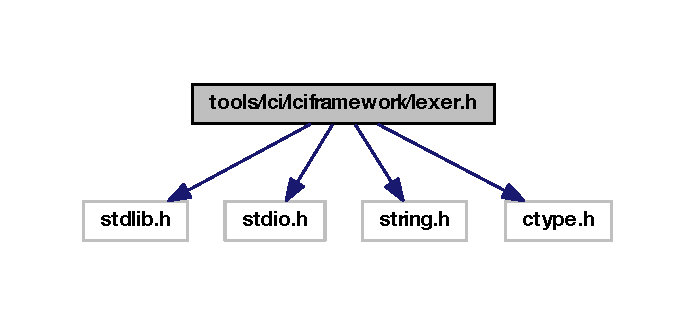
\includegraphics[width=333pt]{lexer_8h__incl}
\end{center}
\end{figure}
This graph shows which files directly or indirectly include this file\-:
\nopagebreak
\begin{figure}[H]
\begin{center}
\leavevmode
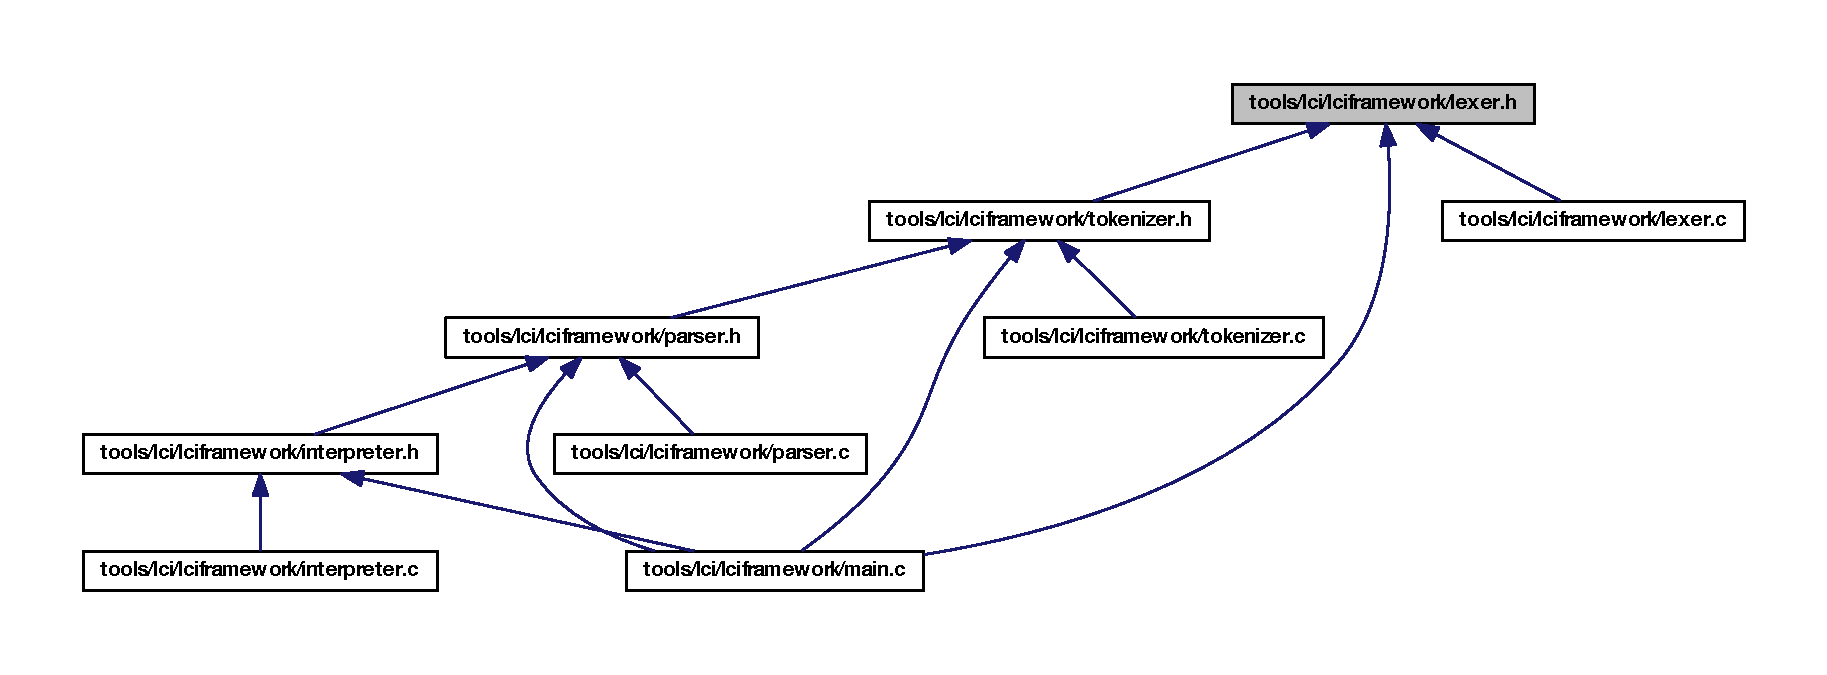
\includegraphics[width=350pt]{lexer_8h__dep__incl}
\end{center}
\end{figure}
\subsection*{Classes}
\begin{DoxyCompactItemize}
\item 
struct \hyperlink{struct_lexeme}{Lexeme}
\item 
struct \hyperlink{struct_lexeme_list}{Lexeme\-List}
\end{DoxyCompactItemize}
\subsection*{Functions}
\begin{DoxyCompactItemize}
\item 
\hyperlink{struct_lexeme}{Lexeme} $\ast$ \hyperlink{lexer_8h_a3133eb4c254d75c6d0a5fd1e9c316784}{create\-Lexeme} (char $\ast$, const char $\ast$, unsigned int)
\item 
void \hyperlink{lexer_8h_a4391032df55eda3e7768792818a7737a}{delete\-Lexeme} (\hyperlink{struct_lexeme}{Lexeme} $\ast$)
\item 
\hyperlink{struct_lexeme_list}{Lexeme\-List} $\ast$ \hyperlink{lexer_8h_a03a7275accd6e39d369c689760bd15df}{create\-Lexeme\-List} (void)
\item 
\hyperlink{struct_lexeme}{Lexeme} $\ast$ \hyperlink{lexer_8h_af9ec30b004772b01fb38f6dc4f54d102}{add\-Lexeme} (\hyperlink{struct_lexeme_list}{Lexeme\-List} $\ast$, \hyperlink{struct_lexeme}{Lexeme} $\ast$)
\item 
void \hyperlink{lexer_8h_a3a834cd76633550e9b8be7368cdeae3d}{delete\-Lexeme\-List} (\hyperlink{struct_lexeme_list}{Lexeme\-List} $\ast$)
\item 
\hyperlink{struct_lexeme_list}{Lexeme\-List} $\ast$ \hyperlink{lexer_8h_af36072386b3b9de0e932afcd33db5169}{scan\-Buffer} (const char $\ast$, unsigned int, const char $\ast$)
\end{DoxyCompactItemize}


\subsection{Detailed Description}
Structures and functions for separating a character buffer into lexemes. The lexer reads through a buffer of characters (themselves typically read from standard input), strips whitespace, and breaks them up into logical atoms of character strings which, in turn, may be passed on to later processes (such as a tokenizer).

\begin{DoxyAuthor}{Author}
Justin J. Meza
\end{DoxyAuthor}
\begin{DoxyDate}{Date}
2010 
\end{DoxyDate}


Definition in file \hyperlink{lexer_8h_source}{lexer.\-h}.



\subsection{Function Documentation}
\hypertarget{lexer_8h_af9ec30b004772b01fb38f6dc4f54d102}{\index{lexer.\-h@{lexer.\-h}!add\-Lexeme@{add\-Lexeme}}
\index{add\-Lexeme@{add\-Lexeme}!lexer.h@{lexer.\-h}}
\subsubsection[{add\-Lexeme}]{\setlength{\rightskip}{0pt plus 5cm}{\bf Lexeme}$\ast$ {\bf add\-Lexeme} (
\begin{DoxyParamCaption}
\item[{{\bf Lexeme\-List} $\ast$}]{list, }
\item[{{\bf Lexeme} $\ast$}]{lexeme}
\end{DoxyParamCaption}
)}}\label{lexer_8h_af9ec30b004772b01fb38f6dc4f54d102}
Adds a \hyperlink{struct_lexeme}{Lexeme} structure to a \hyperlink{struct_lexeme_list}{Lexeme\-List} structure.

\begin{DoxyPrecond}{Precondition}
{\itshape list\/} was created by \hyperlink{lexer_8h_a03a7275accd6e39d369c689760bd15df}{create\-Lexeme\-List(void)}. 

{\itshape lexeme\/} was created by \hyperlink{lexer_8h_a3133eb4c254d75c6d0a5fd1e9c316784}{create\-Lexeme(char $\ast$, const char $\ast$, unsigned int)}.
\end{DoxyPrecond}
\begin{DoxyPostcond}{Postcondition}
{\itshape lexeme\/} will be added on to the end of {\itshape list\/} and the size of {\itshape list\/} will be updated accordingly.
\end{DoxyPostcond}
\begin{DoxyReturn}{Returns}
A pointer to the added \hyperlink{struct_lexeme}{Lexeme} structure (will be the same as {\itshape lexeme\/}).
\end{DoxyReturn}

\begin{DoxyRetVals}{Return values}
{\em N\-U\-L\-L} & realloc was unable to allocate memory. \\
\hline
\end{DoxyRetVals}

\begin{DoxyParams}[1]{Parameters}
\mbox{\tt in,out}  & {\em list} & A pointer to the \hyperlink{struct_lexeme_list}{Lexeme\-List} structure to add {\itshape lex\/} to. \\
\hline
\mbox{\tt in}  & {\em lexeme} & A pointer to the \hyperlink{struct_lexeme}{Lexeme} structure to add to {\itshape list\/}. \\
\hline
\end{DoxyParams}


Definition at line 83 of file lexer.\-c.

\hypertarget{lexer_8h_a3133eb4c254d75c6d0a5fd1e9c316784}{\index{lexer.\-h@{lexer.\-h}!create\-Lexeme@{create\-Lexeme}}
\index{create\-Lexeme@{create\-Lexeme}!lexer.h@{lexer.\-h}}
\subsubsection[{create\-Lexeme}]{\setlength{\rightskip}{0pt plus 5cm}{\bf Lexeme}$\ast$ {\bf create\-Lexeme} (
\begin{DoxyParamCaption}
\item[{char $\ast$}]{image, }
\item[{const char $\ast$}]{fname, }
\item[{unsigned int}]{line}
\end{DoxyParamCaption}
)}}\label{lexer_8h_a3133eb4c254d75c6d0a5fd1e9c316784}
Creates a \hyperlink{struct_lexeme}{Lexeme} structure.

\begin{DoxyReturn}{Returns}
A pointer to a \hyperlink{struct_lexeme}{Lexeme} structure with the desired properties.
\end{DoxyReturn}

\begin{DoxyRetVals}{Return values}
{\em N\-U\-L\-L} & malloc was unable to allocate memory.\\
\hline
\end{DoxyRetVals}
\begin{DoxySeeAlso}{See also}
\hyperlink{lexer_8h_a4391032df55eda3e7768792818a7737a}{delete\-Lexeme(\-Lexeme $\ast$)} 
\end{DoxySeeAlso}
\begin{DoxyNote}{Note}
fname is not copied because it would only one copy is stored for all \hyperlink{struct_lexeme}{Lexeme} structures that share it. 
\end{DoxyNote}

\begin{DoxyParams}[1]{Parameters}
\mbox{\tt in}  & {\em image} & An array of characters that describe the lexeme. \\
\hline
\mbox{\tt in}  & {\em fname} & A pointer to the name of the file containing the lexeme. \\
\hline
\mbox{\tt in}  & {\em line} & The line number from the source file that the lexeme occurred on. \\
\hline
\end{DoxyParams}


Definition at line 10 of file lexer.\-c.

\hypertarget{lexer_8h_a03a7275accd6e39d369c689760bd15df}{\index{lexer.\-h@{lexer.\-h}!create\-Lexeme\-List@{create\-Lexeme\-List}}
\index{create\-Lexeme\-List@{create\-Lexeme\-List}!lexer.h@{lexer.\-h}}
\subsubsection[{create\-Lexeme\-List}]{\setlength{\rightskip}{0pt plus 5cm}{\bf Lexeme\-List}$\ast$ {\bf create\-Lexeme\-List} (
\begin{DoxyParamCaption}
\item[{void}]{}
\end{DoxyParamCaption}
)}}\label{lexer_8h_a03a7275accd6e39d369c689760bd15df}
Creates a \hyperlink{struct_lexeme_list}{Lexeme\-List} structure.

\begin{DoxyReturn}{Returns}
A pointer to a \hyperlink{struct_lexeme_list}{Lexeme\-List} structure with the desired properties.
\end{DoxyReturn}

\begin{DoxyRetVals}{Return values}
{\em N\-U\-L\-L} & malloc was unable to allocate memory.\\
\hline
\end{DoxyRetVals}
\begin{DoxySeeAlso}{See also}
\hyperlink{lexer_8h_a3a834cd76633550e9b8be7368cdeae3d}{delete\-Lexeme\-List(\-Lexeme\-List $\ast$)} 
\end{DoxySeeAlso}


Definition at line 59 of file lexer.\-c.

\hypertarget{lexer_8h_a4391032df55eda3e7768792818a7737a}{\index{lexer.\-h@{lexer.\-h}!delete\-Lexeme@{delete\-Lexeme}}
\index{delete\-Lexeme@{delete\-Lexeme}!lexer.h@{lexer.\-h}}
\subsubsection[{delete\-Lexeme}]{\setlength{\rightskip}{0pt plus 5cm}void {\bf delete\-Lexeme} (
\begin{DoxyParamCaption}
\item[{{\bf Lexeme} $\ast$}]{lexeme}
\end{DoxyParamCaption}
)}}\label{lexer_8h_a4391032df55eda3e7768792818a7737a}
Deletes a \hyperlink{struct_lexeme}{Lexeme} structure.

\begin{DoxyPrecond}{Precondition}
{\itshape lexeme\/} points to a \hyperlink{struct_lexeme}{Lexeme} structure created by \hyperlink{lexer_8h_a3133eb4c254d75c6d0a5fd1e9c316784}{create\-Lexeme(char $\ast$, const char $\ast$, unsigned int)}.
\end{DoxyPrecond}
\begin{DoxyPostcond}{Postcondition}
The memory at {\itshape lexeme\/} and all of its elements will be freed.
\end{DoxyPostcond}
\begin{DoxySeeAlso}{See also}
\hyperlink{lexer_8h_a3133eb4c254d75c6d0a5fd1e9c316784}{create\-Lexeme(char $\ast$, const char $\ast$, unsigned int)} 
\end{DoxySeeAlso}
\begin{DoxyNote}{Note}
We do not free ($\ast$lex)-\/$>$fname because it is shared between many \hyperlink{struct_lexeme}{Lexeme} structures and is free'd by whoever created them. 
\end{DoxyNote}


Definition at line 43 of file lexer.\-c.

\hypertarget{lexer_8h_a3a834cd76633550e9b8be7368cdeae3d}{\index{lexer.\-h@{lexer.\-h}!delete\-Lexeme\-List@{delete\-Lexeme\-List}}
\index{delete\-Lexeme\-List@{delete\-Lexeme\-List}!lexer.h@{lexer.\-h}}
\subsubsection[{delete\-Lexeme\-List}]{\setlength{\rightskip}{0pt plus 5cm}void {\bf delete\-Lexeme\-List} (
\begin{DoxyParamCaption}
\item[{{\bf Lexeme\-List} $\ast$}]{list}
\end{DoxyParamCaption}
)}}\label{lexer_8h_a3a834cd76633550e9b8be7368cdeae3d}
Deletes a \hyperlink{struct_lexeme_list}{Lexeme\-List} structure.

\begin{DoxyPrecond}{Precondition}
{\itshape list\/} was created by \hyperlink{lexer_8h_a03a7275accd6e39d369c689760bd15df}{create\-Lexeme\-List(void)} and contains items added by \hyperlink{lexer_8h_af9ec30b004772b01fb38f6dc4f54d102}{add\-Lexeme(\-Lexeme\-List $\ast$, Lexeme $\ast$)}.
\end{DoxyPrecond}
\begin{DoxyPostcond}{Postcondition}
The memory at {\itshape list\/} and any of its associated members will be freed.
\end{DoxyPostcond}
\begin{DoxySeeAlso}{See also}
\hyperlink{lexer_8h_a03a7275accd6e39d369c689760bd15df}{create\-Lexeme\-List(void)} 
\end{DoxySeeAlso}

\begin{DoxyParams}[1]{Parameters}
\mbox{\tt in,out}  & {\em list} & A pointer to the \hyperlink{struct_lexeme_list}{Lexeme\-List} structure to delete. \\
\hline
\end{DoxyParams}


Definition at line 110 of file lexer.\-c.

\hypertarget{lexer_8h_af36072386b3b9de0e932afcd33db5169}{\index{lexer.\-h@{lexer.\-h}!scan\-Buffer@{scan\-Buffer}}
\index{scan\-Buffer@{scan\-Buffer}!lexer.h@{lexer.\-h}}
\subsubsection[{scan\-Buffer}]{\setlength{\rightskip}{0pt plus 5cm}{\bf Lexeme\-List}$\ast$ {\bf scan\-Buffer} (
\begin{DoxyParamCaption}
\item[{const char $\ast$}]{buffer, }
\item[{unsigned int}]{size, }
\item[{const char $\ast$}]{fname}
\end{DoxyParamCaption}
)}}\label{lexer_8h_af36072386b3b9de0e932afcd33db5169}
Scans through a character buffer, removing unecessary characters and generating lexemes. Lexemes are separated by whitespace (but newline characters are kept as their own lexeme). String literals are handled a bit differently\-: starting at the first quotation character, characters are collected until either an unescaped quotation character is read (that is, a quotation character not preceeded by a colon which itself is not proceeded by a colon) or a newline or carriage return character is read, whichever comes first. This handles the odd case of strings such as \char`\"{}\-::\char`\"{} which print out a single colon. Also handled are the effects of commas, ellipses, and bangs (!).

\begin{DoxyPrecond}{Precondition}
{\itshape size\/} is the number of characters starting at the memory location pointed to by {\itshape buffer\/}.
\end{DoxyPrecond}
\begin{DoxyReturn}{Returns}
A pointer to a \hyperlink{struct_lexeme_list}{Lexeme\-List} structure. 
\end{DoxyReturn}

\begin{DoxyParams}[1]{Parameters}
\mbox{\tt in}  & {\em buffer} & An array of characters to tokenize. \\
\hline
\mbox{\tt in}  & {\em size} & The number of characters in {\itshape buffer\/}. \\
\hline
\mbox{\tt in}  & {\em fname} & An array of characters representing the name of the file used to read {\itshape buffer\/}. \\
\hline
\end{DoxyParams}


Definition at line 135 of file lexer.\-c.


\input{tokenizer_8h}
\input{unicode_8h}
\printindex
\end{document}
